\documentclass[a4paper]{report}
\usepackage[margin=3.5cm,top=2.8cm,bottom=2.8cm]{geometry} %,top=0.5cm,bottom=1.8cm]{geometry}
\usepackage[pdftex]{hyperref}
\usepackage[svgnames]{xcolor}

\usepackage[numbers]{natbib}
\bibliographystyle{plainnat}

% \usepackage{fontspec} % allows Unicode fonts
% \setmainfont{Noto Color Emoji} % or any emoji-capable font

\usepackage{amsmath,amsfonts,amssymb,amsthm,mathtools,thmtools,thm-restate,cleveref}
\usepackage{bookmark,graphicx,dsfont,datetime,float,booktabs,enumitem,outlines,nicematrix}
\usepackage{tabto,caption}
\usepackage{algorithm,algpseudocode}
\usepackage{tabularx,ragged2e,adjustbox} % for literature table
\usepackage{tocloft}    % customize toc entries
\usepackage{xpatch}     % for bookmark 'hack' for appendix naming
\usepackage{setspace}   % for bookmark fix of bibliography
\usepackage{mdframed}   % for "emphasis boxes"

\usepackage{pdfcomment} % adding floating pdf comments
\newcommand{\comment}[1]{\pdfmargincomment[author=Jeroen van Riel]{#1}}

\usepackage{tikz}
\usetikzlibrary{calc, positioning, fit, backgrounds, spy}

% micro-level typesetting
\usepackage[activate={true,nocompatibility},final,tracking=true,kerning=true,spacing=true,
            factor=500,stretch=15,shrink=15]{microtype}

% theorem environments
\theoremstyle{definition}
\newtheorem{eg}{Example}[chapter]
\newtheorem{define}{Definition}[chapter]
\theoremstyle{plain}
\newtheorem{proposition}{Proposition}[chapter]
\newtheorem{lemma}{Lemma}[chapter]
\newtheorem{corollary}{Corollary}[chapter]
\newtheorem{theorem}{Theorem}[chapter]
\newtheorem{assump}{Assumption}[chapter]
\newtheorem{remark}{Remark}[chapter]

% cref settings
\crefname{equation}{equation}{equations}
\newcommand{\crefrangeconjunction}{--}

% load styling for knitr produced tables
\definecolor{fgcolor}{rgb}{0.345, 0.345, 0.345}
\newcommand{\hlnum}[1]{\textcolor[rgb]{0.686,0.059,0.569}{#1}}%
\newcommand{\hlstr}[1]{\textcolor[rgb]{0.192,0.494,0.8}{#1}}%
\newcommand{\hlcom}[1]{\textcolor[rgb]{0.678,0.584,0.686}{\textit{#1}}}%
\newcommand{\hlopt}[1]{\textcolor[rgb]{0,0,0}{#1}}%
\newcommand{\hlstd}[1]{\textcolor[rgb]{0.345,0.345,0.345}{#1}}%
\newcommand{\hlkwa}[1]{\textcolor[rgb]{0.161,0.373,0.58}{\textbf{#1}}}%
\newcommand{\hlkwb}[1]{\textcolor[rgb]{0.69,0.353,0.396}{#1}}%
\newcommand{\hlkwc}[1]{\textcolor[rgb]{0.333,0.667,0.333}{#1}}%
\newcommand{\hlkwd}[1]{\textcolor[rgb]{0.737,0.353,0.396}{\textbf{#1}}}%
\let\hlipl\hlkwb

\usepackage{framed}
\makeatletter
\newenvironment{kframe}{%
 \def\at@end@of@kframe{}%
 \ifinner\ifhmode%
  \def\at@end@of@kframe{\end{minipage}}%
  \begin{minipage}{\columnwidth}%
 \fi\fi%
 \def\FrameCommand##1{\hskip\@totalleftmargin \hskip-\fboxsep
 \colorbox{shadecolor}{##1}\hskip-\fboxsep
     % There is no \\@totalrightmargin, so:
     \hskip-\linewidth \hskip-\@totalleftmargin \hskip\columnwidth}%
 \MakeFramed {\advance\hsize-\width
   \@totalleftmargin\z@ \linewidth\hsize
   \@setminipage}}%
 {\par\unskip\endMakeFramed%
 \at@end@of@kframe}
\makeatother

\definecolor{shadecolor}{rgb}{.97, .97, .97}
\definecolor{messagecolor}{rgb}{0, 0, 0}
\definecolor{warningcolor}{rgb}{1, 0, 1}
\definecolor{errorcolor}{rgb}{1, 0, 0}
\newenvironment{knitrout}{}{} % an empty environment to be redefined in TeX


\DeclareMathOperator{\interior}{int}
\DeclareMathOperator*{\argmax}{arg\,max}
\DeclareMathOperator*{\argmin}{arg\,min}
\newcommand\halfopen[2]{\ensuremath{[#1,#2)}}
\newcommand\openhalf[2]{\ensuremath{(#1,#2]}}
\newcommand*\diff{\mathop{}\!\mathrm{d}}

\newcommand\note[1]{{\color{Navy}\noindent#1}}
\newcommand\smallnote[1]{{\color{Navy}\noindent\scriptsize#1}}

\definecolor{review}{HTML}{8c1f85}
\newcommand\review[1]{{\color{review}#1}}

\newcommand{\TUE}{TU\kern-0.12em/\kern-0.08eme }

% set title, date and author
\newdateformat{monthyeardate}{\monthname[\THEMONTH] \THEYEAR}
\author{\Large Jeroen van Riel \\[6em] {\it Combined Master's Thesis} \\[0.6em] Industrial and Applied Mathematics \\ Computer Science and Engineering  \\[3em] {\it Supervisors} \\[0.6em] Marko Boon \\ Stella Kapodistria \\ Mykola Pechenizkiy \\ Danil Provodin  \\[8em] October 2025 \\[0.6em] Eindhoven University of Technology}
\date{}
\newcommand{\mytitle}{\huge \bf Reinforcement Learning for Combinatorial Optimization in Autonomous Traffic Coordination}

\title{\mytitle}

% set pdf meta-data
\hypersetup{
    pdftitle = {\mytitle},
    pdfauthor = {Jeroen van Riel}
}

\begin{document}

%
% title page
%
\noindent\makebox[\textwidth][c]{%
  \begin{minipage}[h]{\textwidth}
  \note{[ parts that will probably change and comments are in blue ]}\\
  \review{[ parts that the reviewer may want to revisit are in purple ]}
  \maketitle
  \end{minipage}
}

\chapter*{Abstract}
\note{
Coordination schemes for autonomous vehicles offer clear advantages over
conventional traffic management.
%
When considering the problem of optimizing the joint trajectories of individual
autonomous vehicles, we identify some fundamental computational challenges.
%
Ordering and prioritization decisions arise naturally in this context, since
infrastructure must be shared among multiple vehicles.
%
The combinatorial complexity of these decisions rules out simple enumeration
procedures for finding optimal solutions.
%
Furthermore, the infinite-dimensional nature of trajectories complicates
the application of standard combinatorial optimization techniques.

To explore these challenges, we consider a simple model of autonomous traffic
coordination in a network of intersections, where determining the order in which
vehicles cross each intersection on their route is the main combinatorial
component.
%
To enable precise and interpretable results, we consider a traffic system where
all vehicles are autonomous and homogeneous in terms of dimensions and dynamics.
Each vehicle follows its own fixed route through the network and its speed
profile is controlled by a central coordination algorithm, assuming perfect
communication without loss or delay.
%
In this setting, we stage the traffic coordination task as a trajectory
optimization problem.

For a single isolated intersection, we show that---under certain
assumptions---the optimization problem admits a bilevel decomposition into (i)
an upper-level scheduling problem of determining crossing times at the
intersection and (ii) a set of lower-level trajectory optimization problems.
%The feasibility of the lower-level problems is characterized by a system of
%linear inequalities in terms of crossing times.
%
The lower-level problems can be solved relatively efficiently using standard
numerical methods.
%
The upper-level problem can be solved using mixed-integer linear programming,
but this does not scale very well to more vehicles.

To address this scalability issue, we investigate how machine learning can be
employed to develop smart heuristics for the upper-level problem.
%
We show that crossing time schedules can be interpreted as a sequence of
decisions.
%
We propose a sequence model with a simple recurrent neural network
parameterization, which we fit on optimal schedules obtained through
mixed-integer linear programming.
%
The resulting heuristic achieves an optimality gap of up to 2\%, with
near-instant evaluation time compared to mixed-integer linear programming.
%
However, this supervised learning regime still depends on our ability to obtain
optimal schedules for training.
%
To overcome this limitation, we show that we can use reinforcement learning to
train the sequence model from scratch.
%
Both training regimes produce heuristics that outperform a commonly used greedy
scheduling heuristic.

Extending our methodology to multiple intersections introduces additional
complexity. In particular, it becomes more involved to guarantee feasibility of
the lower-level problems due to the finite capacity of lanes between
intersections.
%
We find that this feasibility is characterized by a system of linear
inequalities in terms of the crossing times, which enables the bilevel
decomposition to extend to the network case.
%
Consequently, the corresponding scheduling problem can again be approached as a
sequence modeling task.
%
Compared to the single intersection case, the results show that this case is
much harder.
%
A possible explanation is found in the redundancy of the sequence encoding of
schedules---multiple sequences correspond to the same schedule---which makes
learning inefficient.
%
We find that the order in which the model is evaluated matters for the final
performance, confirming previous observations and motivating further research on
alternative encodings. }

%
% table of contents setup
%

% 'parts' in toc without page numbers
% the 'Part' text is included manually
\cftpagenumbersoff{part}
\renewcommand{\cftpartfont}{\color{red!70!black}}
\renewcommand{\cftpartpresnum}{}

% exclude part level in pdf bookmarks
\makeatletter
\renewcommand{\toclevel@part}{100}
\makeatother

% numbers before each chapter/section in pdf bookmarks
\bookmarksetup{
  numbered,
}

% greyed out leader dots
\renewcommand{\cftdot}{\textcolor{gray!70}{.}}

\newpage
\tableofcontents

% add toc entry in pdf bookmarks
\addtocontents{toc}{\protect{\pdfbookmark[0]{\contentsname}{toc}}}


% \chapter*{Preface}
% \addcontentsline{toc}{chapter}{\protect\numberline{}Preface}


% All hand-drawn figures in this thesis were produced by the Ipe extensible
% drawing editor\footnote{\url{https://ipe.otfried.org}}.



\chapter{Introduction}

\section{Motivation and challenges}

%%% motivation:

% natural to study aut. coord.
% define "coordination"
%
Given the ongoing advances in self-driving vehicles and wireless communication,
it is very natural and relevant to study how these technologies and capabilities
can be employed to improve road traffic.
%
One of the promising possibilities is \emph{coordination of groups of vehicles},
by which we mean the dynamic management of interactions among vehicles and
between vehicles and infrastructure, to align their behaviors---such as speed,
routing, and maneuvers---in a way that promotes safety, efficiency, and smooth
traffic flow.

% studied from wide range of perspectives, methods
%
The general goal of coordination has been approached from a wide range of
perspectives, which has given rise to diverse concrete problem formulations and
methodologies.
%
The level of organization at which coordination takes place is a very typical
distinguishing feature among existing
works~\cite{marianiCoordinationAutonomousVehicles2022}.
%
A well-known example of \emph{local coordination} is platooning of vehicles, in
which consecutive vehicles on the same lane try to keep close together while
maintaining similar speeds, with the aim of lowering energy consumption by
reducing aerodynamic resistance. It has been shown that platooning can also
result in a more efficient use of
intersections~\cite{miculescuPollingsystemsbasedAutonomousVehicle2016,tachetRevisitingStreetIntersections2016,timmermanPlatoonFormingAlgorithms2021}.
On a larger scale, \emph{global coordination} methods like dynamic route
optimization have been proposed to reduce travel delay for all vehicles in the
network~\cite{rossiRoutingAutonomousVehicles2018}.

% many modeling aspects
%
Apart from the level of organization, coordination problems can have many more
modeling aspects. For example, one may think of heterogeneous vehicles---in
terms of physical differences or functionality---different models of
centralized/decentralized communication between vehicles or with the
infrastructure, under different guarantees on reliability; complex road
topology, curved lanes affecting the maximum safe speed, merging lanes;
implications of mixing human traffic with fully autonomous traffic.
%
We will discuss some common modeling aspects in the literature review below.

% even simple models provide fundamental computational challenges
%
Although coordination has been considered from various angles, some fundamental
challenges related to safety and efficiency remain poorly understood, even in
stylized models with the bare minimal modeling elements such as vehicle dynamics
and collision-avoidance constraints.
%
This brings us to the scope of this project.
%
% define project scope
%
In order to better understand these inherent difficulties and to enable us to
obtain concrete interpretable results, we focus on \emph{fully automated
  mobility systems}, in which all vehicles are assumed to have autonomous driving
and communication capabilities.
%
Since we are specifically interested in coordination across multiple vehicles,
we assume that the lower-level steering control of individual vehicles is taken
care of; we assume that vehicles can follow planned trajectories perfectly.
%
% further motivation: such systems actually exist
%
Even though this model does not capture many of the intricacies of our current
road network, there are many examples in which such a model is appropriate. For
example, think of autonomous vehicles being deployed in so-called confined
sites, like ports, mines or quarries; but also warehouses and manufacturing
sites, or even indoor farming installations.
%
% further motivation: upper bounds
%
Moreover, even in the context of urban road traffic, stylized models are
relevant, because they provide upper bounds on what we can expect to gain in
more realistic situations with, e.g., decentralized control, random failures and
problems like communication latency and noisy information.

% focus on optimization of motion
%
We will take an \emph{optimization-based planning perspective} on the
coordination problem, in which the joint trajectories of the vehicles in the
system are our main decisions.
%
% challenge: defining the constraints and optimization objective
%
In this context, there are some natural requirements and objectives, which are
often conflicting with each other.
%
First of all, guarantees of safety and collision avoidance are fundamental issues.
%
From the perspective of promoting traffic throughput of the system, minimizing
travel delay is a very natural objective. However, there is a tension with the
goal of limiting fuel and energy consumption.
%
In multi-user systems like traffic networks, attention to fairness is also
of central importance.
%
Other objectives like passenger comfort, e.g., with smooth
acceleration/deceleration, have also been considered in this context.
%
Apart from the difficulty of formulating the optimization problem and its
objective function, the following challenges have been identified with respect
to the algorithmic aspects of solving such optimization problems.

% \begin{figure}
%   \centering
%   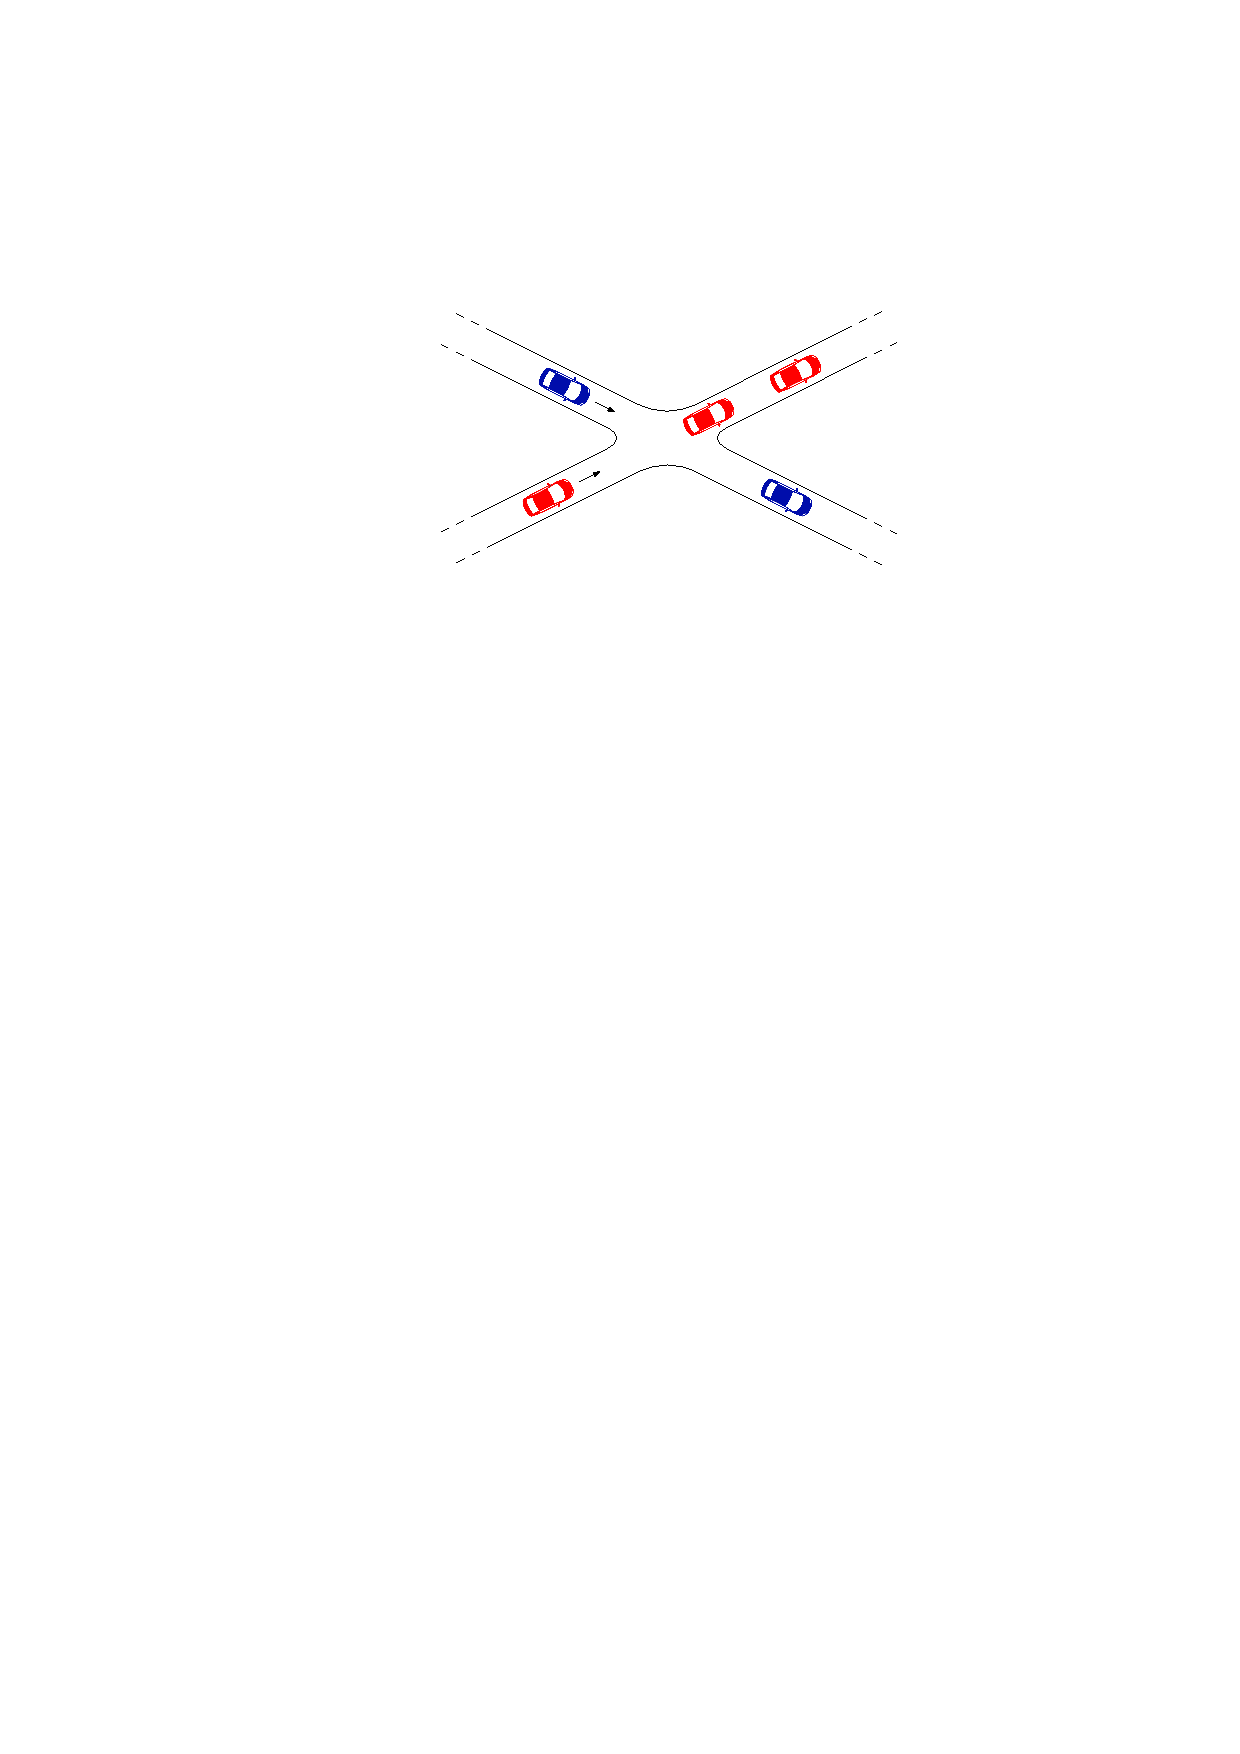
\includegraphics[scale=1]{figures/intersection-nice}
%   \caption{Stylized model of a single intersection with two conflicting flows
%     that do not merge, so we assume vehicles must cross the intersection in a
%     straight line, without turning.}
% \end{figure}

%%% general challenges (within the context of optimization-based coordination):

\paragraph{Complex combinatorial decisions.}

In traffic coordination, combinatorial problems arise naturally from ordering
constraints---deciding which vehicle should move first across shared resources
such as intersections, merge areas, or lanes, while taking into account trade-offs
between throughput, fairness, and safety.
%
Traditionally, such problems are resolved by implementing traffic lights or
static rules for yielding.
%
Autonomous connected vehicles provide us with better ways of handling these
conflicts dynamically.

For example, we will focus specifically on the order in which vehicles cross
intersections, which can also be thought of as grouping vehicles into platoons
and then deciding in which order these platoons are allowed to cross the
intersection.
%
Instead of relying on fixed traffic signal phases, we can optimize this decision
for the current traffic situation.
%
Other examples include determining the optimal order of vehicles in a
platoon that is approaching an intersection with dedicated lanes for turning.
%
On a higher level, determining the routes that vehicles take is a classical
combinatorial optimization problem, think for example of the traveling salesman
problem.

Even when vehicle routes are fixed, such ordering decisions at one intersection
directly influence the arrival process at nearby intersections, hence these
decisions are coupled across the network.
%
Due to this coupling, finding the optimal crossing plan becomes harder when
larger networks are considered, because of the exponential growth of the space
of feasible solutions.
%
This issue is further complicated by the real-time requirement that real traffic
systems impose on the computation time.

\paragraph{Continuous-time trajectories under constraints.}

We are dealing with the optimization of vehicle trajectories, which is in
general an infinite-dimensional problem.
%
Such problems can be approached in an end-to-end fashion by
\textit{direct transcription} to an equivalent mixed-integer optimization
problem, which can be solved using off-the-shelf solvers. This method can be
used to compute optimal trajectories up to any precision, by choosing a fine
enough time discretization. However, it is exactly this time discretization that
causes prohibitive growth of the number of variables with respect to the size of
the network and the number of vehicles, so this method is only useful for
relatively small problem instances.
%
Moreover, in the context of traffic systems, there are complex constraints and
safety requirements that need to be handled with care.
%
Furthermore, optimization methods would benefit a lot from closed-form
expressions of trajectories, which is in principle possible in some situations,
but the appearance of constraints makes this notoriously difficult in practice.

\paragraph{Joint optimization is hard.}

There are lots of well-understood solution techniques for purely combinatorial
problems.
%
However, in the current context, the combinatorial part of the problem cannot be
considered in isolation. The feasibility and cost of each solution to the
combinatorial part depends in a non-trivial way on the lower-level
continuous-time dynamics and interactions between vehicles.
%
In other words, simultaneously optimizing the combinatorial part and the
continuous-time part, to which we refer as \emph{joint optimization}, poses
major algorithmic challenges.
%
In the literature, heuristics have been studied, often based on the presumption
of decentralized control and communication.
%
However, works in which the combinatorial aspects and the lower-level
continuous-time trajectories are optimized in a unified fashion, in which the
trade-offs that are made can be clearly identified, are scarce in the current
literature.

\section{Literature review}
This section presents a general overview of the relevant literature on
\emph{optimization-based methods for traffic coordination in fully automated
  mobility systems}. Background and literature on the specific
\emph{methodologies} that we will use in this thesis are provided at the
beginning of each chapter or section where we first need it.

In presenting the literature, we group works according to their most salient
feature---be it a specific modeling choice, an algorithmic technique, or a focus
on particular issue.
%
\note{Other common features that are worth mentioning are reservation-based policies,
use of mixed-integer linear programming, fixed ordering policies instead of
optimization, fixed signal phases, platoon-based heuristics.}

Before we discuss exemplary works, we mention some existing surveys that we have
consulted when conducting this literature review.
%
The survey \cite{marianiCoordinationAutonomousVehicles2022} classifies works
mainly on the level of organization. Moreover, apart from vehicle motion around
intersections and other conflict spaces, they also review other interesting
coordination challenges in autonomous traffic management, like smart parking and
ride sharing, which also have significant societal impact.
%
More specifically focused on autonomous intersection management
are~\cite{khayatianSurveyIntersectionManagement2020}, where works are
classified, first on level of organization, but they also consider vehicle
dynamics, conflict detection and scheduling policy.


\paragraph{Reservation-based systems.}
% adjacent: auction, bidding, fairness

Instead of an optimization-based perspective, many studies assume that
vehicles communicate with a central intersection controller to reserve time and
space in the conflict area.
%
The major downside of this line of work is that there is generally no precise
control over the trajectories that vehicles take.

The seminal ``Autonomous Intersection Management'' (AIM) model ~\cite{dresnerMultiagentTrafficManagement2004,dresnerMultiagentApproachAutonomous2008} is a
good example of the reservation-based approach.
%
In this framework, vehicles that want to cross the intersection send a request
to the central controller to occupy the cells containing their trajectory for a
certain amount of time. The central controller then decides to grant or deny
these requests based on previously granted requests to facilitate collision-free
trajectories. If a request is denied, the vehicle slows down and attempts to
obtain a new reservation after some timeout.
%
Note that in the original setting, the central controller does not have complete
control over the precise trajectories that vehicles take; each vehicle agent is
more or less able to decide their own optimal speed profile.
%
However, the central controller does impose some constraints on the acceleration
profile inside the intersection to promote throughput.

Various improvements have been made to the original AIM model to improve the
efficiency of the reservation protocol, for example, by having vehicles make
better estimations of their expected time of arrivals to make more accurate
reservations~\cite{auMotionPlanningAlgorithms2010}.
%
Other works consider speed profile recommendations and more fine-grained
prioritization of requests by the intersection
controller~\cite{huangAssessingMobilityEnvironmental2012}.
%
The model has also been extended to networks of intersections, where dynamic
route optimization has been considered as well~\cite{hausknechtAutonomousIntersectionManagement2011}.
%
Later works propose more precise methods for conflict detection than the
original cell-based approach~\cite{levinConflictpointFormulationIntersection2017,liTemporalspatialDimensionExtensionbased2019}.
%
Finally, communication delays play a major role in practice, so a time-aware
extension of AIM has been introduced
in~\cite{khayatianCrossroadsTimeawareApproach2020}.


\paragraph{Optimizing the crossing order.}

Rather than obtaining a crossing order as the result of a sequence of granted
reservation requests, later studies assume that the intersection manager
explicitly optimizes the sequence in which vehicles cross. Most of these works
also address the online setting, accounting for the random arrival of vehicles
over time.
%
In this online setting, the general goal is to find a \emph{schedule} of
crossing times for the current vehicles in the system and update this schedule
every time new arrivals happen, which is the task of the central \emph{crossing
  time scheduling policy}.

% rolling-horizon optimization
A common method to design such a scheduling policy is to use
\emph{rolling-horizon optimization}. For example, taking the AIM model as a
starting point, a paradigm shift from reservation requests to \emph{assignments}
has been proposed in~\cite{levinConflictpointFormulationIntersection2017}, where
a a mixed-integer linear program is solved in a rolling-horizon fashion to
determine the best assignments.
%
A similar approach is described
in~\cite{liTemporalspatialDimensionExtensionbased2019}, but they formulate the
reservation assignment problem as a non-linear optimization problem, which is
solved using a tabu search heuristic.

% bubbles paper
The policy in~\cite{tallapragadaHierarchicaldistributedOptimizedCoordination2017} deals explicitly with the complexity of the crossing order
decisions by defining groups of consecutive vehicles on the same lane. The first
step is to group vehicles into these so-called ``bubbles''. All vehicles in a
bubble are required to cross the intersection together, while maintaining
feasibility with respect to safe trajectories. Next, crossing times are assigned
to bubbles while avoiding collisions. Based on this schedule, a local vehicular
control method~\cite{tallapragadaDistributedControlVehicle2017} is used that guarantees safety to reach the assigned
crossing times.

% miculescu
The work~\cite{miculescuPollingsystemsbasedAutonomousVehicle2016} considers the scheduling policy in the context of a polling
model, where the intersection, its inbound lanes and vehicles are modeled as
server, queues and customers, respectively.
%
Roughly speaking, each time a new vehicle arrives to the system, the crossing
order may be adapted, which is done by simulating a polling policy.
%
They show that if the polling policy satisfies some regularity condition and if
the lanes are long enough, then every updated crossing order is feasible, in the
sense that vehicles in the system that have been assigned a later crossing time
than before are able to decelerate in time to avoid collisions.
%
The generation of continuous-time vehicle trajectories satisfying these crossing
times is handled by numerically solving an optimal control problem.
% timmerman
Building on this work, it has been shown that these trajectories can also be
computed directly using closed-form
expressions~\cite{timmermanPlatoonFormingAlgorithms2021}.

% joshi
Finally, we note that crossing order decisions become particularly interesting
when vehicles with heterogeneous dimensions and dynamics are considered, which
has been investigated in~\cite{joshiTrajectoriesPlatoonformingAlgorithm2025}.
For example, it makes intuitively sense to assign heavy trucks with slow
acceleration/deceleration characteristics to a dedicated lane to avoid
interfering with passenger vehicles that are more agile.

\paragraph{Joint optimization and decomposition methods.}

Finally, we mention some of the few works that have considered the joint
optimization perspective, which has also been called ``signal-vehicle coupled
control (SVCC)''. The prominent theme here is trying to come up with good
approximation algorithms. A central idea in this line of work is trying to
exploit somehow the fact that the problem can be formulated in terms of a
decomposition of the upper-level crossing time scheduling problem and
lower-level problems for generating continuous-time trajectories.

% Hult et al. (offline single intersection with energy objective)
% "An approximate solution to the optimal coordination problem for autonomous
% vehicles at intersections"
The approximation method in~\cite{hultApproximateSolutionOptimal2015} is based
on a bilevel decomposition and considers a quadratic objective involving
velocity as a proxy for energy. The first stage optimizes a schedule of vehicle
crossing times. It uses approximations of each vehicle's contribution to the
total objective as a function of its crossing time. Next, for each vehicle, the
second stage computes an optimal trajectory satisfying the crossing time
schedule, by solving a quadratic program. This approach has been shown to reduce
running times significantly. Unfortunately, the study is limited to a single
intersection and it is assumed that each lane approaching the intersection
contains exactly one vehicle.

% Zhao et al. (bilevel programming model)
The paper~\cite{zhaoBilevelProgrammingModel2021} proposes a trajectory
optimization scheme for a single intersection, also based on the bilevel
decomposition. The lower-level problem is employed to maximize the speed at
which vehicles enter the intersection. Both parts of the problem are solved in an alternating
fashion, each time updating the constraints of the other part based on the
current solution.

\note{\paragraph{Identified gaps.} Add a small summary to synthesize the key gaps in the literature.}

% \newcolumntype{L}[1]{>{\RaggedRight\hsize=#1\hsize\hspace{0pt}}X}
% \begin{table}[t]
% \centering
% \renewcommand{\arraystretch}{1.2}

% \begin{adjustbox}{center}
% \scalebox{0.7}{
% \begin{tabularx}{2.0\textwidth}{@{} l L{0.6} L{0.55} L{0.55} L{0.55} L{0.55} L{0.55} L{1.0} @{}}
% \toprule
% \textbf{Ref.} &
% \textbf{Paradigm} &
% \textbf{Dynamics} &
% \textbf{Safety} &
% \textbf{Objective} &
% \textbf{Decision set} &
% \textbf{Communication} &
% \textbf{Notes / Limitations} \\
% \midrule
% \cite{dresnerMultiagentApproachAutonomous2008} &
% Reservation-based &
% Planar vehicle kinematics &
% Conflict exclusion (grid cells) &
% Delay minimization &
% Entry times/reservation slots &
% Multiagent with central intersection manager &
% Simplified vehicle model; global heuristic \\
% \bottomrule
% \end{tabularx}}
% \end{adjustbox}
% \caption{Comparison of approaches to signal-free intersection management.}
% \label{tab:litreview}
% \end{table}

\section{Project goals and outline}

% \paragraph{Research goals and questions.}

From the start of this project, the overarching goal has been to develop
tractable optimization models and algorithms for the coordination of automated
vehicles at intersections.
%
% is some history appropriate here?
%
In the initial phase, we considered dynamic and stochastic aspects like random
vehicle arrivals. However, after reviewing the current state of the literature,
we realized that there are still many unresolved issues in the deterministic
settings.
%
In the end, this project has been centered around the following two general
goals related to coordination of autonomous vehicles:

% problem-directed goals
\begin{enumerate}[label=\textbullet, leftmargin=3em, rightmargin=4em]
  \item \emph{Develop a simplified yet representative mathematical optimization model
        for coordination of autonomous vehicles in networks of intersections.}

  \item \emph{Understand the inherent algorithmic challenges that complicate joint
        optimization of crossing order and generation of continuous-time
        trajectories.}
\end{enumerate}

Complementary to these problem-driven goals, the work presented in this thesis
has also been inspired by some developments in applying machine learning methods
to combinatorial optimization.
%
% [insert brief discussion of those methods and results]
% refer to appendix for further background
%
\note{[ this needs a little more introduction ]}
Motivated by these recent successes, we also aim to \emph{illustrate the use of
  such machine learning algorithms to obtain heuristics for combinatorial problems arising in the context of coordinating autonomous
  vehicles}.

% research questions: concrete, addressable
To make the above broad goals concrete and addressable, our work has been guided
by the following research questions:

\begin{enumerate}[label=RQ\arabic*:, leftmargin=3em, rightmargin=4em]
  \item How can the autonomous traffic coordination problem with
        collision-avoidance constraints at a single isolated intersection be
        formulated in an optimization framework for multiple autonomous
        vehicles? (modeling)

  \item Under which assumptions can the combinatorial aspect of determining the
        crossing order be considered in isolation? (decomposition)

  \item What is the relative computational complexity of solving the
        combinatorial problem compared to solving the continuous-time trajectory
        optimization, given the crossing order? (complexity)

  \item How to leverage the recent successes in applying machine learning for
        combinatorial optimization to solve the combinatorial problems arising
        in the context of autonomous traffic management? (heuristics)

  \item How to extend the previous questions to a network of multiple connected
        intersections? (scalability)
\end{enumerate}

% concrete goals/research questions:
% - scalable coordination algorithm
% - real-time computational requirements
% - not completely model-free, but partly model-based to exploit apparant structure


The contributions of this work can be summarized into three main categories:
\note{More appropriate in the conclusion chapter?}

\paragraph{(i). Isolating the combinatorial problem.}
Deciding the crossing order of vehicles at intersections is a central challenge
in traffic management. This holds especially for when considering multiple lanes
and intersections.
%
However, after fixing these ordering decisions, the remaining problem is often
much easier to solve. This observation motivates the decomposition of the
trajectory optimization problem into two parts.
%
The upper-level problem determines the times at which vehicles cross the
intersections on their routes, to which we will refer as \emph{crossing times}.
%
Once these are fixed, we solve a set of lower-level problems to find the
corresponding vehicle trajectories satisfying the crossing times.
%
Our first contribution is to show that, under certain conditions, our joint
trajectory optimization problem for vehicles in a network of intersections
decomposes into an upper-level crossing time scheduling problem and a set of
lower-level trajectory optimization problems. We show that feasibility of the
upper-level scheduling problem is completely characterized in terms of a system
of linear inequalities involving the crossing times. This allows us to first
solve the scheduling problem and then generate trajectories for it once we have
the optimal crossing time schedule.

\paragraph{(ii). Learning-based scheduling.}
Our second contribution is an illustration of how machine learning techniques
can be applied to solve scheduling problems in practice, using our crossing time
scheduling problem as a case study.
%
Many practical instances of combinatorial problems contain structure that
classic solutions techniques try to exploit, e.g., by defining smart heuristics
based on human intuition and experience.
%
A recent trend in the literature has been to aim for automation of this manual
endeavor, for example by formulating parametric sequence models to capture the
conditional probability of optimal solutions, given a problem instance.
%
Specifically, we recognize that the solution of the crossing time scheduling
problem can be interpreted as a sequence of decisions.
%
Instead of manually trying to develop good heuristics and algorithms, we try to
learn what optimal solutions are, by treating it as a learning task on
sequences.
%
As has been noted before, we confirm that the order of evaluation during
inference matters a lot for the final solution quality.

\paragraph{(iii). Coordination across multiple intersections.}
We show a way to extend isolated intersection coordination to multi-intersection
networks. We show under which assumptions this problem can still be formulated
as a scheduling problem, which turns out to be an extension of the classical job
shop scheduling problem.
%
In this setting, feasibility of trajectories deserves special attention.

\paragraph{Outline.}

In Chapter~\ref{chap:single}, we consider a simple model of a single
intersection, like the example above. After discussing the decomposition method,
we present some classical solutions methods to solve the crossing time
scheduling problem.
%
We explain how the problem can be treated as a learning problem in
Chapter~\ref{chap:single-learning}.
%
In order to generalize to a network of intersections, we need to give a precise
characterization of the feasibility of trajectories in lanes of finite length,
which is done in Chapter~\ref{chap:network}.
%
The resulting scheduling problem is then subjected to a learning algorithm in
Chapter~\ref{chap:network-learning}.
%
We provide some general discussion and pointers for further research in
Chapter~\ref{chap:conclusion}.




\microtypesetup{deactivate}
\part*{\hspace*{-0.8em}\textsc{Part I}\\[0.6em] Isolated Intersection\\[3em]
       \centering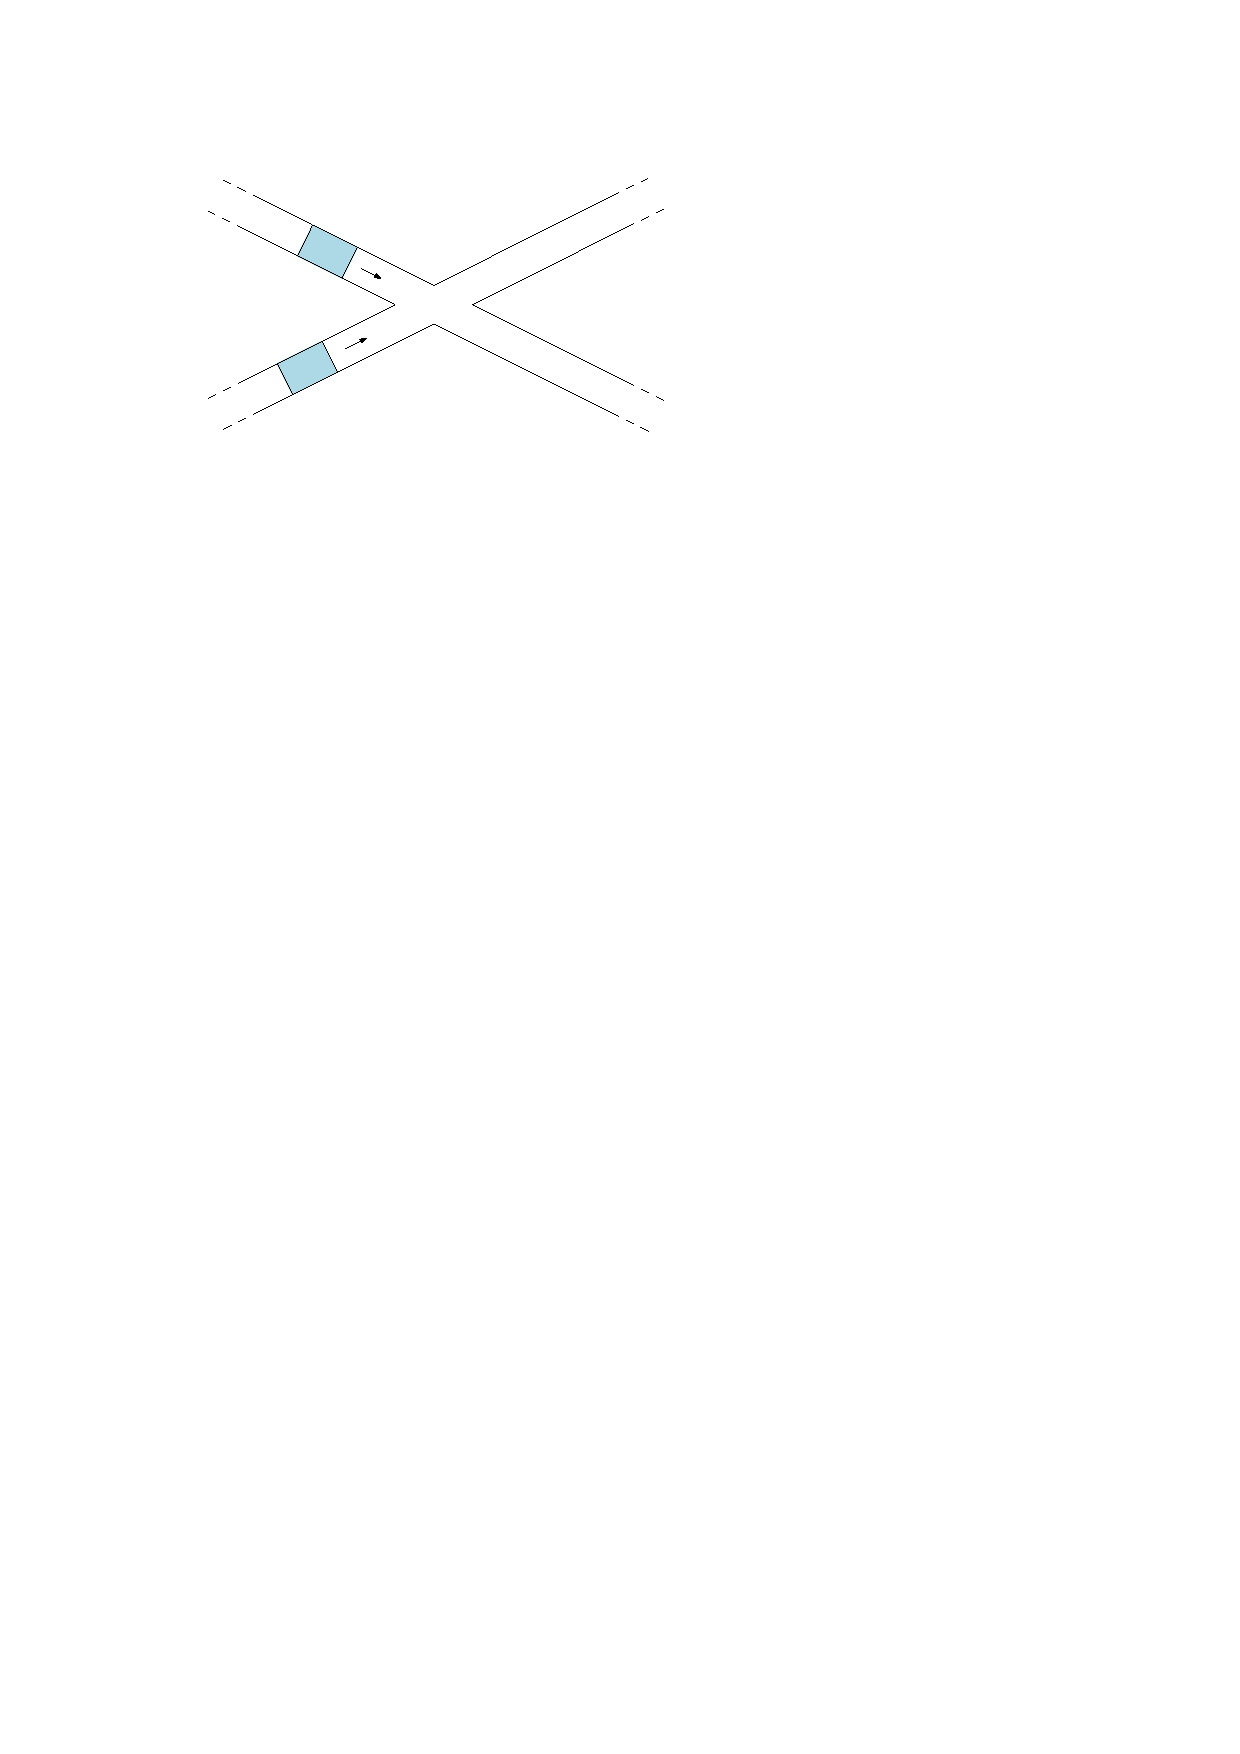
\includegraphics[scale=1]{figures/intersection-non-axis-aligned}}
\microtypesetup{activate}
\addcontentsline{toc}{part}{Part I \;--\; Isolated Intersection}



\chapter{Isolated intersection scheduling}\label{chap:single}

% broad problem:
% - why intersections matter in traffic coordination
% - why coordination is interesting

% simpflified model as a tractable starting point
% assumptions:
% - two lanes
% - perpendicular
% - no turning
% - no overtaking
% - homogeneous vehicles (same dimensions and dynamics)
% - no randomness
%  - fixed

% optimization objective:
%   - energy consumption -> very desirable on top of delay, but makes analysis difficult
%   - travel delay -> essential, enables problem simplification (decomposition)

% mathematical punchline:
% - first, it becomes a trajectory optimization problem (optimal control)
%   - can be solved directly
% - next, we turn it into a very simple scheduling (when) / sequencing (only order) problem

% preview of results:
% - mention direct transcription
% - main takeaway: bilevel decomposition
% - branch-and-cut solution
%   - problem structure yields cutting planes
%   - analye performance improvement
% - optionally, mention local search

% broad problem
Efficient coordination of vehicle motion at intersections has been and still is
a central challenge in traffic management, because intersections are natural
bottlenecks where safety requirements and efficiency objectives are directly in
conflict.
%
With the advent of automated vehicles and reliable wireless communication
technologies, there is increasing potential to replace traditional traffic
signal-based approaches with coordinated trajectory planning methods.
%
Our literature review clearly shows that previous works have approached
coordination of automated vehicles from a wide range of perspectives and with
varying degrees of model complexity.
%
Furthermore, we highlighted some fundamental computational challenges that are
still unresolved in the literature.
%
Specifically, the joint optimization of crossing order and continuous-time
vehicle trajectories has received relatively little attention.
%
In order to better understand this issue and to enable precise analytical
results, we propose to study a stylized single intersection model.

% mathematical punchline
Formulated mathematically, coordination of automated vehicles at a single
intersection can be expressed as a problem of \emph{trajectory optimization},
which we will make precise in Section~\ref{sec:intersection-model}.
%
In this formulation, the accelerations of all vehicles are chosen to satisfy
their dynamics and collision-avoidance requirements while minimizing some
cost function.
%
% optimization objectives
The following two conflicting cost components are of primary interest:
%
minimizing travel delay, which is essential for capturing the efficiency of
traffic flow; and minimizing energy consumption, which is highly desirable in
practice because it supports sustainability.

% direct transcription to bilevel decomposition (general) to proper decomposition (assumptions+delay)
Trajectory optimization problems of this type can be solved directly using
general-purpose optimization schemes based on time discretization.
%
As we will illustrate in Section~\ref{sec:direct-transcription}, such methods
are straightforward to implement and guarantee to find an optimal solution to
the joint optimization problem. However, their running time scales very poorly
when considering finer discretization grids or when increasing the number of
vehicles in the system, motivating the development of tailored algorithms that
exploit the structure of the problem.

Given the observation that each feasible set of trajectories implicitly fixes
some order in which vehicles cross the intersection, it is natural to ask
whether this ordering decision can be considered separately.
%
In general, the answer is negative; in other words, we cannot first optimize the
crossing order, then compute the corresponding continuous-time vehicle
trajectories.
%
Still, this decomposition idea is a helpful way to think about the problem, so
it is discussed extensively in Section~\ref{sec:bilevel}.

\emph{It turns out that a proper decomposition is possible}, if we use a cost
function that only involves delay and if we are willing to impose the additional
constraint that vehicles need to cross the intersection at full speed. For this
case, we show in Section~\ref{sec:delay-minimization} that the original
infinite-dimensional trajectory optimization problem essentially reduces to a
finite-dimensional \emph{scheduling problem}, in which only the sequencing of
vehicles and their entry times into the intersection need to be determined.
%
Scheduling problems like this have been studied extensively and can be solved
using off-the-shelf methods like mixed-integer linear programming, which we
illustrate in Section~\ref{sec:crossing-time-scheduling}.
%
By leveraging insight into the structure of optimal solutions, we are able to
formulate three problem-specific cutting planes, yielding an efficient
algorithm for coordination at a single intersection.

\begin{remark}
  The main starting point of this chapter will be a continuous-time trajectory
  optimization problem, which is typically studied in the framework of optimal
  control theory. Since the author does not have a strong background in this
  field, the aim is not to provide a rigorous treatment from this perspective.
  %
  Nevertheless, we want to be as precise and complete as possible, because this
  trajectory optimization problem is the basis for our further development.
  %
  Therefore, at some points in this chapter, remarks are included regarding the
  subleties of our formulation, most notably, regarding the occurrence of
  so-called state constraints.
\end{remark}

\begin{figure}
  \centering
  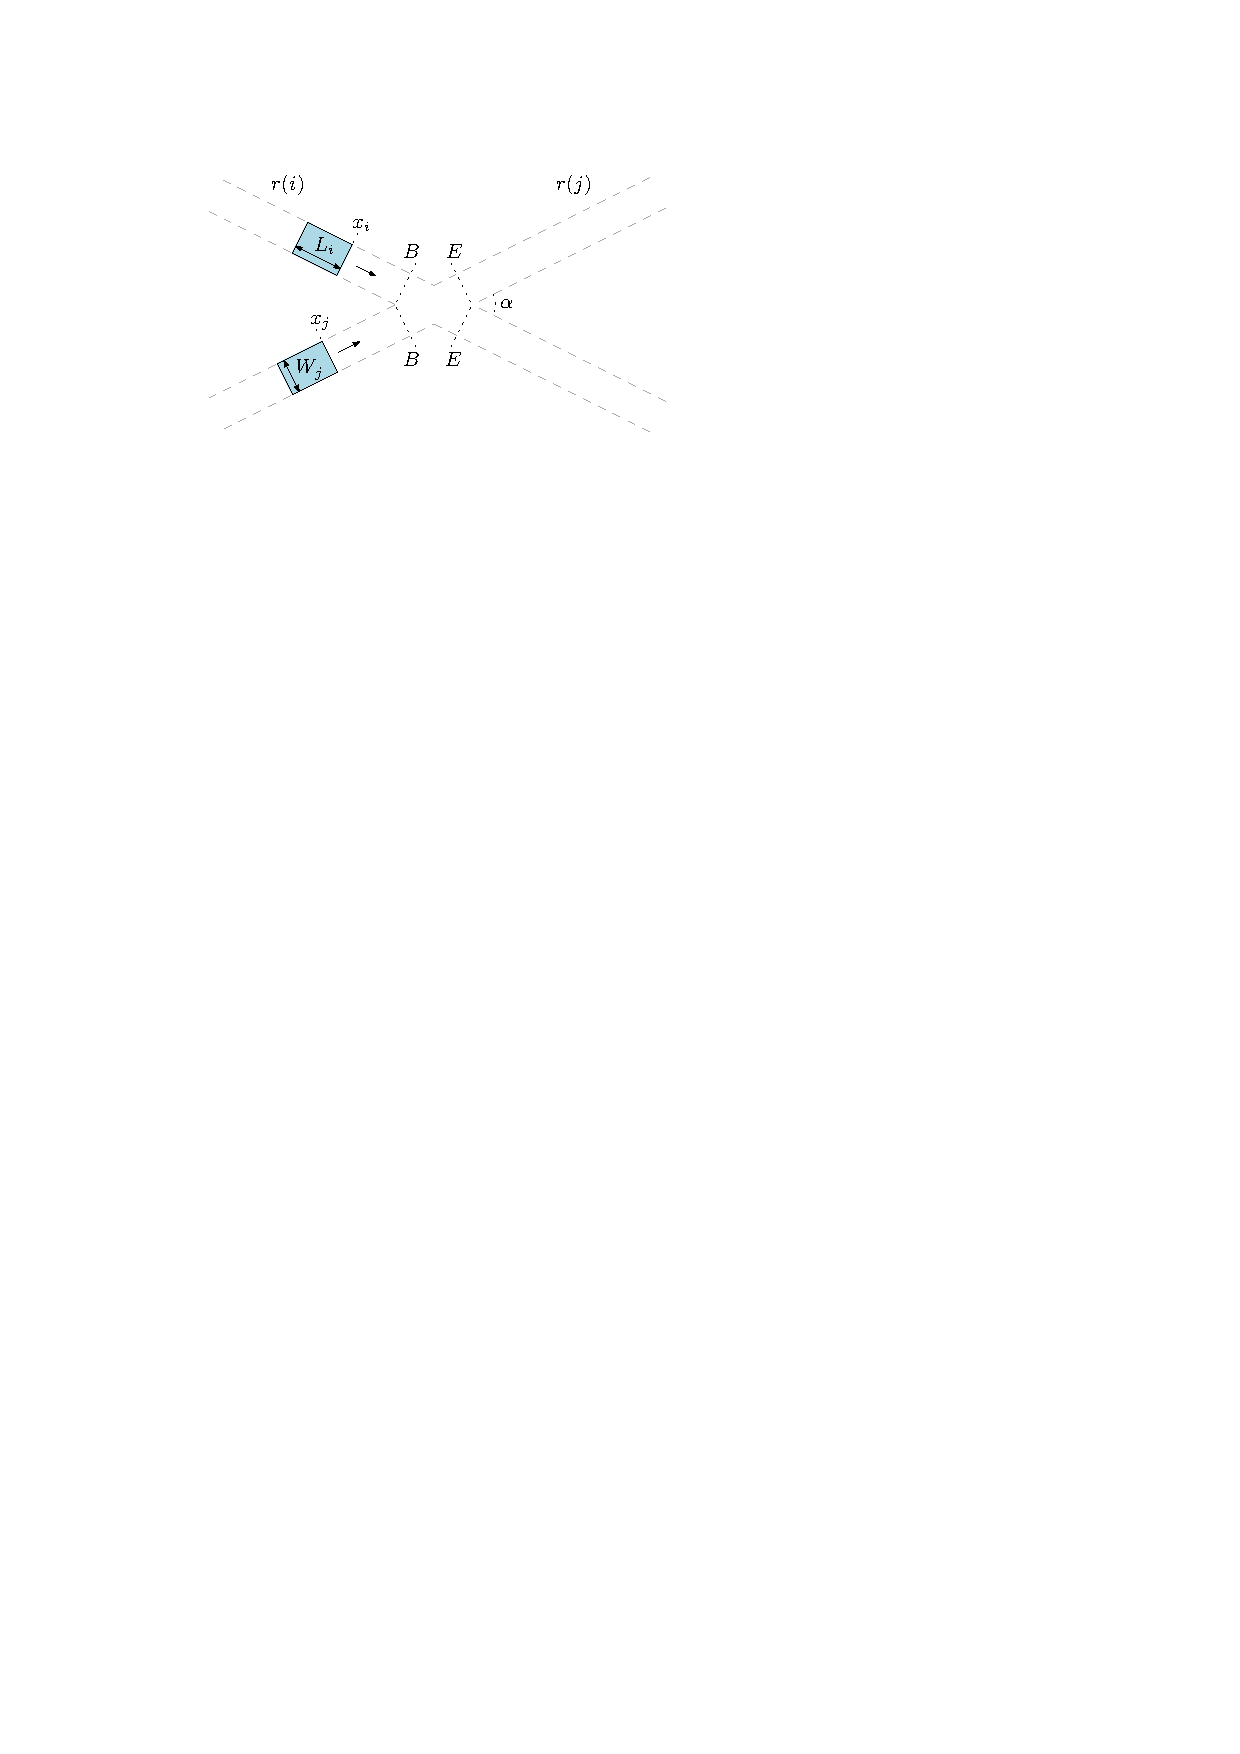
\includegraphics[scale=1]{figures/intersection-non-axis-aligned-annotated}
  \caption{Example of two vehicle routes intersecting at some angle $\alpha$. The
    indicated positions $x_{i} = B$ and $x_{i} = E$ for each vehicle $i$ are
    chosen such that whenever the vehicle position $x_{i}$ satisfies either
    $x_{i} \leq B$ or $x_{i} - L_{i} \geq E$, then the intersection area is not
    occupied by this vehicle at all and the other vehicle can take any position
    without causing a collision.}%
  \label{fig:intersection-non-axis-aligned}
\end{figure}


\section{Intersection model}\label{sec:intersection-model}

% model assumption to make analysis tractable
To make the analysis tractable, we restrict our attention to intersections of
single-lane roads on which vehicles are traveling without turning maneuvers or
overtaking.
%
All vehicles are assumed to be homogeneous, sharing identical dimensions and
dynamics, so that their motion can be modeled uniformly.
%
A central controller determines the acceleration, and thus the speed, of each
vehicle, under the assumption of perfect communication.
%
Moreover, we do not consider randomness in arrivals or dynamics, so we assume
that each vehicle's initial state is known precisely such that the system
evolves deterministically as a function of the acceleration control inputs.

We start by defining the geometry of the intersection and the vehicles and
analyze the resulting conflict-free joint positions of all the vehicles in the
system.
%
After that, we introduce the dynamics of the system and define several objective
functions to arrive at the trajectory optimization problem.

\paragraph{Valid configurations.}
%
We model each vehicle $i$ in the plane as some rigid body $\mathcal{B}_{i}$
traveling along some straight line $r(i)$, to which we will refer as the
vehicle's \emph{route}.
%
We will assume that vehicles always stay on their route and thus do not make
turning maneuvers.
%
Therefore, the longitudinal position of a vehicle along its route can be
represented by some scalar $x_{i} \in \mathbb{R}$.
%
For simplicity, we use a rectangular vehicle geometry, so each $\mathcal{B}_{i}$
is a translated rectangle of width $W_{i}$ and length $L_{i}$. For technical
convenience, we assume this rectangle is an \emph{open} set. We write
$\mathcal{B}_{i}(x_{i})$ to denote the corresponding translated rigid body in
the plane, where $x_{i}$ corresponds to the location of the front bumper; the
rear bumper position is then $x_{i} - L_{i}$.
%
We allow multiple routes to cross in a single point. Of course, this causes some
joint vehicle positions to be invalid, because they would correspond to
collisions.
%
Before we allow arbitrary numbers of vehicles to have the same route, we briefly
investigate the valid configurations of two vehicles, each on its own route.


Consider two routes intersecting at some angle $\alpha$, as illustrated in
Figure~\ref{fig:intersection-non-axis-aligned}, each with a single vehicle on
it. Let these vehicles be denoted as $i$ and $j$.
%
We can try to characterize the set $\mathcal{X}_{ij} \subset \mathbb{R}^{2}$ of
feasible configurations $(x_{i}, x_{j})$ for which these two vehicles are not in
a collision, in the sense that their corresponding translated rigid bodies do
not intersect.
%
In general, this set can thus simply be defined as
\begin{align}
  \label{eq:3}
  \mathcal{X}_{ij} := \{ (x_{i}, x_{j}) \in \mathbb{R}^{2} : \mathcal{B}_{i}(x_{i}) \cap \mathcal{B}_{j}(x_{j}) = \varnothing \} .
\end{align}
%
However, it is often easier to take the opposite perspective, by characterizing
the set of conflicting configurations $\mathcal{X}_{ij}^{C}$. \comment{Nice, ``C''
  for conflict and for complement!}

% discuss rectangular subset of configuration space
%
In the situation with two routes, we fix two reference positions $B$ and $E$ on
each route, delimiting the intersection area as shown in
Figure~\ref{fig:intersection-non-axis-aligned}.
%
These positions are chosen such that whenever $x_{i} \leq B$ or
$x_{i} - L_{i} \geq E$, it is clear that vehicle $i$ does not occupy the intersection
at all, so the other vehicle $j$ is free to take any position
$x_{j} \in \mathbb{R}$.
%
Thus, we obtain the following conservative approximation of the set of conflicting
configurations:
\begin{align}\label{eq:conf-space-approx}
  (B,E + L_{i}) \times (B, E + L_{j}) \supseteq \mathcal{X}_{ij}^{C} .
\end{align}
Of course, the set of feasible configurations is generally a little larger and
depends on the angle $\alpha$ of intersection, as illustrated by the three examples
in Figure~\ref{fig:intersection-config-spaces}.
%
In case of the third example, where the intersections make a right angle
$\alpha = \pi/2$, it it not difficult to see that there is actually equality in~\eqref{eq:conf-space-approx}.

To keep the presentation simple, we will make the following assumption: all
vehicles share the same vehicle geometry, i.e, $L_{i} \equiv L$ and
$W_{i} \equiv W$. As a shorthand of the vehicle positions that correspond to
occupying the intersection area, we will write $\mathcal{E} := (B, E + L)$.
%
This enables us to model any number of intersecting routes, as long as we can
assume that $\mathcal{E}$ provides a conservative approximation of all
intersection-occupying vehicle positions.

\begin{figure}
  \centering
  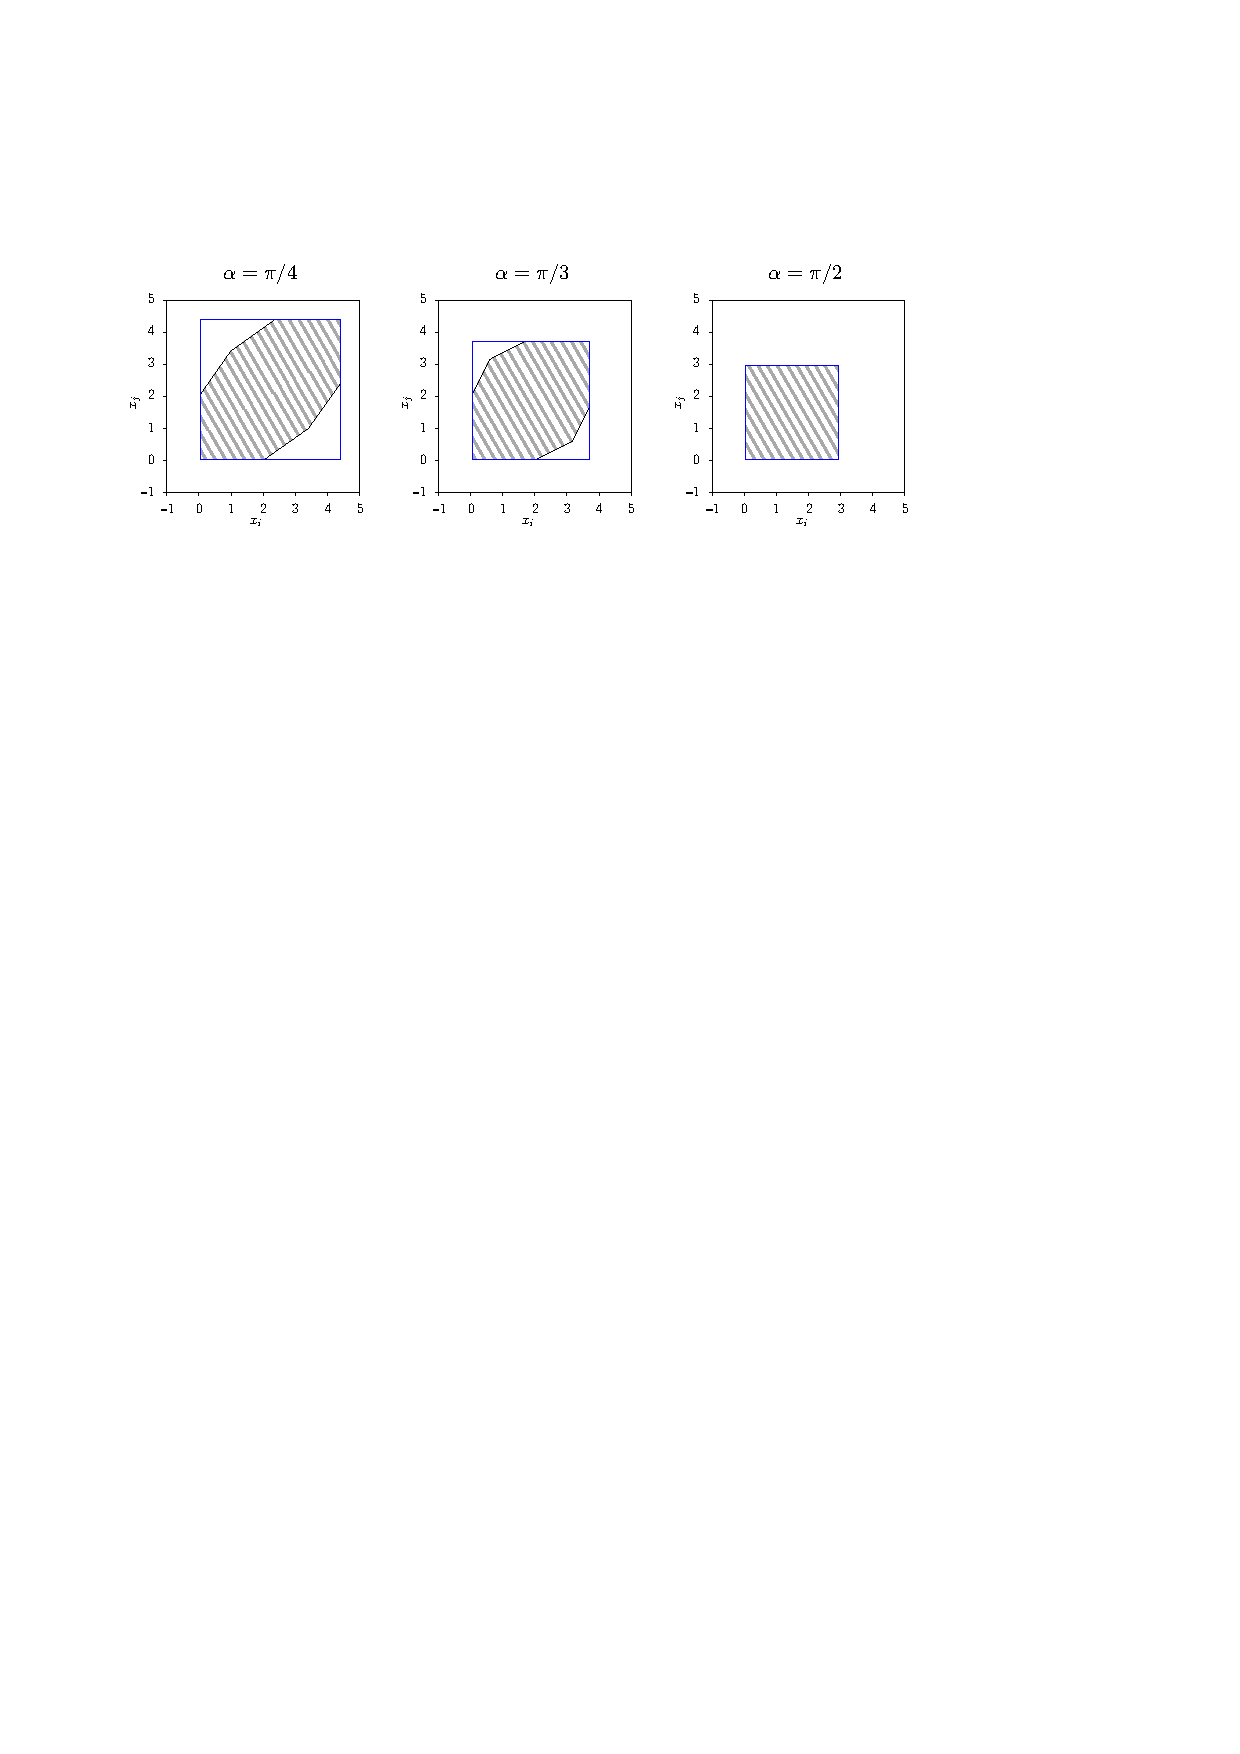
\includegraphics[scale=1]{figures/intersection-config-spaces}
  \caption{For three different intersection angles and fixed vehicle dimensions
    $W_{i} = W_{j} = 1$ and $L_{i} = L_{j} = 2$, we plotted the region
    $\mathcal{X}_{ij}^{C}$ in configuration space corresponding to collisions as
    the area marked in grey. The blue square regions correspond to the
    approximation of the collision area using~\eqref{eq:conf-space-approx}. Because we assume a
    rectangular vehicle geometry, these figures are relatively straightforward
    to compute, which we briefly explain in
    Appendix~\ref{app:configuration-space}.}%
  \label{fig:intersection-config-spaces}
\end{figure}

% collision-avoidance in routes
% \paragraph{Multiple vehicles.}
Let us now proceed to arbitrary numbers of vehicles. We will use the following
notation for identifying routes and vehicles.
%
Let the routes be identified by indices $\mathcal{R} := \{1, \dots, R\}$. Let
$n_{r}$ denote the number of vehicles following route $r$, and let
$N := n_1 + \dots + n_R$ denote the total number of vehicles in the system, for
which we have the set of vehicle indices
\begin{align}
  \mathcal{N} = \{ (r, k) : k \in \{1, \dots, n_{r}\}, r \in \mathcal{R}\} .
\end{align}
Occasionally, we will also write $\mathcal{N}_{r}$ to identify the set of
vehicles on route $r$. Given vehicle index $i = (r, k) \in \mathcal{N}$, we use
the auxiliary notation $r(i) = r$ and $k(i) = k$.

% conjunctions (vehicle following)
In order to maintain a safe distance between successive vehicle on the same
route, it is clear that vehicles need to satisfy the \textit{safe headway constraints}
\begin{align}
  \label{eq:follow_constraints}
  x_{i} - x_{j} \geq L ,
\end{align}
at all times, for all pairs of indices $i, j \in \mathcal{N}$ such that
$r(i) = r(j)$ and $k(i) + 1 = k(j)$. Let $\mathcal{C}$ denote the set of all
such ordered pairs of indices. Note that these constraints restrict vehicles
from overtaking each other, so their initial relative order is always
maintained. In other words, $(i,j) \in \mathcal{C}$ means that $i$ crosses the
intersection before $j$.

% disjunctions (conflicts)
Similarly, let $\mathcal{D}$ denote the set of \emph{conflicts}, which are all
(unordered) pairs of vehicles $i, j \in \mathcal{N}$ on different routes
$r(i) \neq r(j)$.
%
Recall that we introduced $\mathcal{E}$ to denote the interval of positions for
which some vehicle is said to \emph{occupy} the intersection. Then, for each conflict
$\{i,j\} \in \mathcal{D}$, we impose at all times the \emph{safe crossing constraints}
\begin{align}
  \label{eq:2}
  (x_{i}, x_{j}) \notin \mathcal{E}^{2} .
\end{align}

\paragraph{Trajectory optimization.}
Next, we introduce the motion dynamics of the vehicles, so let $x_{i}(t)$ denote
the position of vehicle $i$ at time $t$.
%
Let $\dot{x}_{i}$ and $\ddot{x}_{i}$ denote its speed and acceleration,
respectively, then we consider the bounds
\begin{subequations}\label{eq:vehicle-dynamics}
\begin{alignat}{3}
  0         & \leq & \; \dot{x}_{i}(t)  & \leq && \; \bar{v}  , \label{eq:speed-constr} \\
  {-\omega} & \leq & \; \ddot{x}_{i}(t) & \leq && \; \bar{\omega} ,
\end{alignat}
\end{subequations}
for some positive $\bar{v}, \omega, \bar{\omega} > 0$.
%
Given a pair of initial position and velocity $s_{i} = (x_{i}^{0}, v_{i}^{0})$,
we write $x_{i} \in D(s_{i})$ if and only if the trajectory $x_{i}$ has
$(x_{i}(0), \dot{x}_{i}(0)) = s_{i}$ and satisfies~\eqref{eq:vehicle-dynamics}.

% cost functional
We now present some possible ways of measuring how desirable an individual
vehicle trajectory $x_{i}(t)$ is, by defining a cost functional $J(x_{i})$ that
we aim to minimize.
%
For example, consider the following parametric cost functional
\begin{align}
  J_{\alpha,\beta}(x_{i}) = \int_{0}^{t_{f}} \alpha x_{i}(t) + \beta |\ddot{x}_{i}(t)| \diff t .
\end{align}
%
First of all, note that the absolute value of the acceleration is often used as
a proxy for energy consumption, so $\beta > 0$ is generally desirable.
%
\comment{There are nice physics arguments why one proxy is preferred over the
  other, but we just ignore this.}
%
Minimizing energy is in direct conflict with our other main goal, which is to
reach the intersection in some reasonable amount of time. However, we have not
yet explicitly encoded this.
%
We will explicitly add this goal later, but for now, it is possible to achieve a
similar effect by setting $\alpha < 0$, which may be interpreted as rewarding
trajectories that ``move forward fast'' and is thus a natural choice if we want
to promote overall throughput of the system.
%
Minimizing $J_{\alpha,\beta}$ with $\alpha = -1$ and $\beta = 0$ will be of
particular interest to us later, which we will call the \emph{haste objective},
for ease of reference.
%
To give another example, consider cost functionals of the form
\begin{align}\label{eq:energy-objective}
  J_{v_{d}}(x_{i}) = \int_{0}^{t_{f}} {(v_{d} - \dot{x}_{i}(t))}^{2} + {(\ddot{x}_{i}(t))}^{2} \diff t ,
\end{align}
where $v_{d} > 0$ is some reference velocity. This objective can be interpreted
as trying to maintain a velocity close to $v_{d}$, while simultaneously
minimizing the square of acceleration as proxy of energy consumption.

Given some $J(\cdot)$, we can now conclude our model description by defining the
general trajectory optimization problem.
%
Given the pairs of initial vehicle positions and velocities
$s := \{s_{i} = (x_{i}^{0}, v_{i}^{0}) : i \in \mathcal{N} \}$ and some final
simulation time $t_{f} > 0$, we consider the problem of finding some set
$x = \{ x_{i} : i \in \mathcal{N} \}$ of continuous trajectories $x_{i}$, that
minimize
%
\comment{T for ``trajectory''.}
\begin{alignat}{3}\label{eq:single-trajectory-optimization}
  T(s) := \min_{x} \;\, & \sum_{i \in \mathcal{N}} J(x_{i}) \tag{T} \\
  \text{such that } \; & x_{i} \in D(s_{i}) && \quad \text{ for all } i \in \mathcal{N} , \tag{T.1} \label{eq:T1} \\
  % \text{such that } \; & (x_{i}(0), \dot{x}_{i}(0)) = (x_{i}^{0}, v_{i}^{0}) && \quad \text{ for all } i \in \mathcal{N} ; \nonumber \\
           % \omit\rlap{and for all $t \in [0,t_{f}]$:} \notag \\
           % & \dot{x}_{i}(t) \in [0, \bar{v}]  && \quad \text{ for all } i \in \mathcal{N} , \nonumber \\
           % & \ddot{x}_{i}(t) \in [{-\omega}, \bar{\omega}] && \quad \text{ for all } i \in \mathcal{N} , \nonumber \\
           & x_{i}(t) - x_{j}(t) \geq L && \quad \text{ for all } (i,j) \in \mathcal{C} , \tag{T.2} \label{eq:T2}\\
           & (x_{i}(t), x_{j}(t)) \notin \mathcal{E}^{2} && \quad\text{ for all } \{i, j\} \in \mathcal{D} . \tag{T.3} \label{eq:T3}
\end{alignat}
Our main interest lies in solving this problem for different instances of $s$, the
remaining ``system parameters''
$(L,\mathcal{E}, \bar{v}, \omega, \bar{\omega}, t_{f})$ are mostly assumed to be
fixed.

\begin{remark}
Problem~\eqref{eq:single-trajectory-optimization} is non-convex in some sense;
recall that the set of feasible configurations $\mathcal{X}_{ij}$ for two
vehicles is already non-convex.\comment{I say ``roughly speaking'', because I am
  not sure personally what this even means precisely. My guess is that the set
  of feasible function, which is a subset of some underlying vector space of
  functions, is convex.}
%
An interpretation of this non-convexity is that we must decide which of the
vehicles crosses the intersection first.
%
In the next section, we will discuss ways of dealing with this non-convexity.
\end{remark}

\begin{remark}\label{rem:state-constraints}
  Note that the variables in~\eqref{eq:single-trajectory-optimization} represent
  continuous-time trajectories, so it is an infinite-dimensional optimization
  problem.
  %
  This kind of problems is typically studied in the framework of optimal control theory.
  %
  In this context, the joint position $x = \{x_{i} : i \in \mathcal{N}\}$ is
  referred to as the \emph{state} of the system and
  $\ddot{x} = \{\ddot{x}_{i} : i \in \mathcal{N} \}$ as the \emph{control}.
  %
  In some sense, acceleration is thus understood to be the main input of the system, such that
  vehicle position is indirectly determined by integrating twice. For this reason,
  this simple vehicle dynamics model is commonly referred to as the \emph{double integrator}.
  %
  It is more common to state optimal control problems in terms of finding some
  continuous $x(t) \in \mathbb{R}^{n}$ and integrable $u(t) \in \mathbb{R}^{m}$,
  which need to satisfy the dynamic equations
  \begin{align}\label{eq:general-dynamics}
    \dot{x} = f(t, x, u) , \quad x(t_{0}) = x_{0} , \quad u \in U \subset \mathbb{R}^{m},
  \end{align}
  for some initial state $x_{0}$ and time $t_{0}$ and some (compact) control set
  $U$. Given some final time $t_{f}$, a running cost function $\mathcal{L}$ and
  some terminal cost function $\mathcal{K}$, the goal is to
  \begin{subequations}\label{eq:opt-control}
  \begin{align}
    \min_{x} \; & \int_{t_{0}}^{t_{f}} \mathcal{L}(t, x(t), u(t)) \diff t + \mathcal{K}(t_{f}, x_{f}) , \\
      \textnormal{such that } \, &\eqref{eq:general-dynamics} \textnormal{ holds, } \\
                    & h(x) = 0 , \label{eq:state-constr-eq} \\
                    & g(x) \leq 0 , \label{eq:state-constr-ineq}
  \end{align}
  \end{subequations}
  with some functions $h : \mathbb{R}^{n} \rightarrow \mathbb{R}^{p}$ and
  $g : \mathbb{R}^{n} \rightarrow \mathbb{R}^{q}$ encoding the so-called state
  constraints. Functions $f, g, h$ are usually assumed to possess certain
  regularity or smoothness properties.
  %
  There are general methods to analyze optimal solutions
  of~\eqref{eq:opt-control}, most notably the necessary conditions given by the
  maximum principle of Pontryagin~\cite{liberzonCalculusVariationsOptimal}.
  %
  However, the occurrence of state constraints like~\eqref{eq:state-constr-eq}
  and~\eqref{eq:state-constr-ineq} make such analysis notoriously difficult and
  remains an area of ongoing research~\cite{hartlSurveyMaximumPrinciples1995}.
  %
  For our current problem, note that the collision-avoidance
  constraints~\eqref{eq:T2} and~\eqref{eq:T3}, as well as the speed
  constraint~\eqref{eq:speed-constr} implied in~\eqref{eq:T1}, are all of the
  type~\eqref{eq:state-constr-ineq}.
\end{remark}


\paragraph{Feasibility.}
The existence feasible trajectories in~\eqref{eq:single-trajectory-optimization} generally depends on the initial
state $s$ of vehicles in some non-trivial manner.%
\footnote{Note that we will characterize the feasibility of
  trajectories for a related problem in Chapter~\ref{chap:network}.
%
  The main difference is that the analysis there will not assume that initial
  vehicle states are given, but rather the times at which vehicles enter the
  system.}
%
To give a rough idea, we derive some simple sufficient conditions.
% feasibility assumption
We exclude initial collisions at time $t=0$ by requiring
\begin{align}\label{eq:initially-safe-assumption}
 x_{i}^{0} - x_{j}^{0} \geq L \quad \text{ for all } \quad  (i,j) \in \mathcal{C} .
\end{align}
%
% full acc/dec times and distances
%
Next, observe that the bounds on speed and acceleration imply that it takes at
least $\bar{v}/\omega$ time to fully decelerate from full speed, during which the
vehicle has traveled a distance of $\bar{v}^2/(2\omega)$. Similarly, a full
acceleration from a stop takes $\bar{v}/\bar{\omega}$ time and
$\bar{v}^2/(2\bar{\omega})$ distance.
%
Therefore, by assuming that each vehicle starts at full speed
$v_{i}^{0} = \bar{v}$ and by imposing a minimum distance to the start of the
intersection
\begin{align}\label{eq:initial-safe-stopping-assumption}
  x_{(r,1)}^{0} \leq B - \bar{v}^2/(2\omega) - \bar{v}^2/(2\bar{\omega}),
\end{align}
for each first vehicle on every route
$r \in \mathcal{R}$, we ensure that there is enough room for all vehicles to
come to a full stop. Even further, there is still enough distance for a full
acceleration to reach full speed while crossing the intersection.
%

\begin{assump}\label{assump:feasible}
  The initial states $s=\{s_i = (x_i^0,v_i^0) : i \in \mathcal{N} \}$
  satisfy~\eqref{eq:initially-safe-assumption}
  and~\eqref{eq:initial-safe-stopping-assumption}.
\end{assump}


\pagebreak
\section{Trajectory optimization}

The main goal of this section is to explain how the trajectory optimization
problem~\eqref{eq:single-trajectory-optimization} can be reduced to a scheduling
problem.
%
To motivate this reduction, we first show that the problem can be solved by
employing a numerical method known as \emph{direct transcription}, but we note
that the associated running time is prohibitive in practice.
%
We then show how~\eqref{eq:single-trajectory-optimization} can in general be
rewritten in terms of coupled optimization problems: an upper-level scheduling
problem, dictating the crossing times for all vehicles in the system, and a
lower-level trajectory optimization problem for the vehicles of each route. We
explain how this reformulation has been used as the basis for an approximation
algorithm.
%
Finally, we show which assumptions we have to make in order for the
decomposition to be \emph{proper}, by which we mean that we can first solve the
upper-level problem to find an optimal crossing time schedule, after which the
lower-level problems can be resolved.


\subsection{Joint optimization using direct transcription}\label{sec:direct-transcription}

The key idea of direct transcription is to reformulate the continuous-time
optimal control problem---which is infinite-dimensional---into a
finite-dimensional nonlinear optimization problem by discretizing time into a
grid.
%
At each grid point, the state and control inputs of every vehicle become
decision variables. The vehicle dynamics and the safety requirements, i.e., the
headway and collision-avoidance constraints, can then be imposed directly in
terms of these decisions variables.
%
This approach allows us to capture the full structure of the problem while
making it accessible to modern nonlinear optimization solvers.
%
In what follows, we describe in detail how this general approach can be applied
to problem~\eqref{eq:single-trajectory-optimization} and illustrate its use by
solving some examples for two different cost functionals.

We start by defining a uniform discretization grid. Let $K$ denote the number of
discrete time steps and let $\Delta t$ denote the time step size, then we define
\begin{align}
  \mathbb{T} := \{0, \Delta t, \dots, K \Delta t\} .
\end{align}
%
For each vehicle $i$, we use $x_{i}(t), v_{i}(t)$ and $u_{i}(t)$ to denote,
respectively, the decision variables for position, speed and acceleration.
%
First of all, we impose the initial conditions by simply adding the constraints
$x_{i}(0) = x_{i}^{0}$ and $v_{i}(0) = v_{i}^{0}$ for each $i \in \mathcal{N}$.
%
Using the forward Euler integration scheme, we further relate these three
quantities by adding the constraints
\begin{subequations}
\begin{align}
  x_{i}(t + \Delta t) = x_{i}(t) + v_{i}(t) \Delta t , \\
  v_{i}(t + \Delta t) = v_{i}(t) + u_{i}(t) \Delta t ,
\end{align}
\end{subequations}
for each $t \in \mathbb{T} \setminus \{K\Delta t\}$ and $i \in \mathcal{N}$. Moreover, we directly include
the inequalities $0 \leq v_{i}(t) \leq \bar{v}$ and
${-\omega} \leq u_{i}(t) \leq \bar{\omega}$ to model the vehicle dynamics.
%
For each pair of successive vehicles $(i, j) \in \mathcal{C}$ on the same route,
the safe headway constraints can simply be added as
\begin{align}
  x_{i}(t) - x_{j}(t) \geq L \quad \text{ for each } t \in \mathbb{T}.
\end{align}

Encoding of the safe crossing constraints needs some additional attention,
because they represent a binary ``disjunctive'' decision.
%
Following the approach in~\cite{hultApproximateSolutionOptimal2015}, these disjunctive constraints can be formulated
using the common big-$M$ method with binary decision variables. For each vehicle
$i \in \mathcal{N}$, we introduce two binary decision variables
$\delta_{i}(t), \gamma_{i}(t) \in \{ 0, 1 \}$ and for each conflict $\{i, j\} \in \mathcal{D}$ and
time step $t \in \mathbb{T}$, we introduce the following constraints:
\begin{subequations}\label{eq:collision-avoidance-binary-encoding}
  \begin{align}
  x_{i}(t) &\leq B + \delta_{i}(t) M , \label{eq:order-constr-1} \\
  \quad x_{i}(t) &\geq E + L - \gamma_{i}(t) M , \label{eq:order-constr-2} \\
  & \hspace{-3.8em} \delta_{i}(t) + \delta_{j}(t) + \gamma_{i}(t) + \gamma_{j}(t) \leq 3 , \label{eq:order-constr-3}
  \end{align}
\end{subequations}
where $M$ is some sufficiently large number.
%
The idea behind this encoding is as follows.
%
First, observe that setting $\delta_{i}(t) $ can be thought of as
\emph{deactivating}~\eqref{eq:order-constr-1}, since $M$ is chosen sufficiently
large such that the inequality is trivially true. Analogously, setting
$\gamma_{i}(t) = 1$ deactivates~\eqref{eq:order-constr-2}.
%
Hence, the constraint~\eqref{eq:order-constr-3} can be interpreted as limiting
the number of deactivations to three, which is equivalent to requiring at least
one of the following four inequalities to hold:
\begin{align}
  x_{i}(t) \leq B, \quad x_{j}(t) \leq B , \quad
  x_{i}(t) \geq E + L, \quad x_{j}(t) \geq E + L ,
\end{align}
which means that vehicles $i$ and $j$ cannot both occupy the intersection at the
same time $t$.

In general, the resulting transcribed optimization problem is a mixed-integer
nonlinear program. We consider an small problem instance with five vehicles for
our cost functional $J_{\alpha,\beta}$, for which the optimal trajectories are
shown in Figure~\ref{fig:direct_transcription_example}. \comment{Optionally include running time analysis to
  motivate the need for fast approximations.}

\begin{remark}
  We used the forward Euler integration scheme for sake of a simple
  presentation. However, note that in practice we most likely want to use a more
  numerically stable method like a higher-order Runge-Kutta scheme or by means
  of some spline interpolation technique. We refer to~\cite{Ch10Trajectory} for a light
  introduction to trajectory optimization in general and~\cite{kellyIntroductionTrajectoryOptimization2017} for a tutorial
  on the direct collocation method, which also contains a concise overview of
  different numerical methods (ibid., Section 9).
\end{remark}


\begin{figure}
  \centering
  \begin{minipage}{0.76\textwidth}
  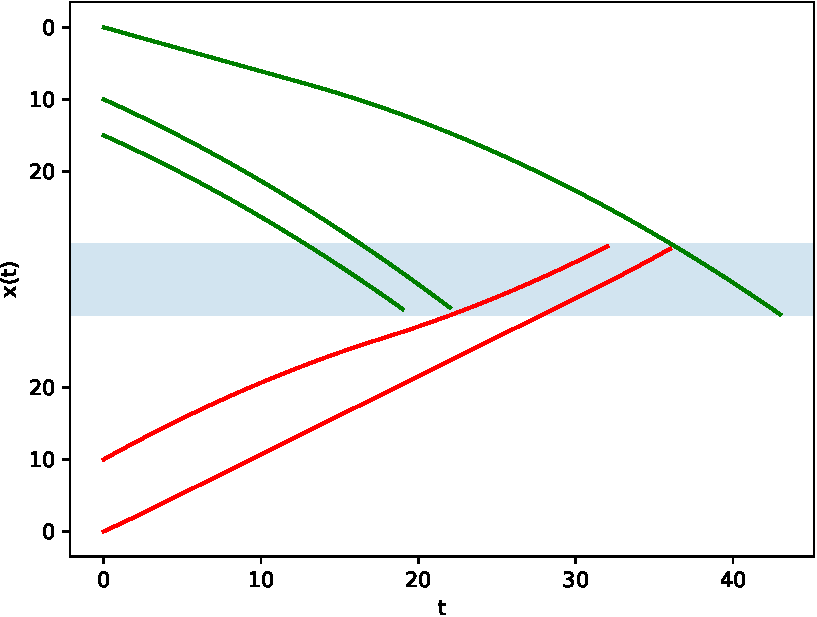
\includegraphics[width=0.9\textwidth]{figures/single/trajectories_general.pdf}%
  \end{minipage}
  \begin{minipage}{0.23\textwidth}
  \vspace*{-1em}
  \begin{tabular}{ c c c }
    $i$ & $x_{i}^{0}$ & $v_{i}^{0}$ \\[0.2em]
    \hline\\[-1em]
    {\color{red}(1,3)} &  0 & 1.0 \\
    {\color{red}(1,2)} & 10 & 1.0 \\
    {\color{red}(1,1)} & 15 & 1.0 \\
    {\color{blue}(2,1)} & 10 & 0.8 \\
    {\color{blue}(2,2)} &  0 & 0.0
  \end{tabular}
  \\[2em]
  \begin{tabular}{ c c c }
    $L$ & = &  5 \\
    $\mathcal{E}$ & = & $[20, 30]$ \\
    $\bar{v}$ & = & 1 \\
    $\omega, \bar{\omega}$ & = & 0.1 \\
    $T$ & = & 50 \\
    $\Delta t$ & = & 1
  \end{tabular}
  \end{minipage}
  \caption{Example of optimal trajectories minimizing $J_{\alpha,\beta}$ (solid)
    and $J_{v_{d}}$ (dashed), obtained using the direct transcription method for
    cost parameters $\alpha = -1, \, \beta = 100$ and $v_{d} = 0.6$. The system
    parameters and initial conditions are listed next to the figure. The y-axis
    is split such that the top part corresponds to route $1$ and the bottom to
    route $2$ and the trajectories are inverted accordingly and drawn with
    separate colors. The interval of intersection-occupying positions
    $\mathcal{E}$ is drawn as a shaded region. We do not draw trajectories
    beyond this region.}%
  \label{fig:direct_transcription_example}
\end{figure}

\subsection{Bilevel decomposition}\label{sec:bilevel}

After applying the transcription method above, the safe crossing constraints of
each conflict are imposed at every time step, requiring a total of $2T$ binary
variables.
%
Therefore, there is some kind of redundancy in this encoding, because the
decision to be made is, in principle, a single binary decision for each
conflict: which of the two vehicle crosses the intersection first?
%
However, a more direct encoding would require decision variables for the time of
entry into and exit out of the intersection for each vehicle.
%
This insight is the key to decomposing the problem into an upper-level problem
and a set of lower-level problems.
%
Roughly speaking, the upper-level problem optimizes the time slots during which
vehicles occupy the intersection, while the lower-level problems produce optimal
safe trajectories that respect these time slots.
%
\comment{c.f. Benders' decomposition}
%
% The following presentation and notation is adapted
% from~\cite{hultApproximateSolutionOptimal2015}.
%

Given some feasible trajectory $x_{i} \in D(s_{i})$ for a single vehicle $i$, we
define its (earliest) \emph{entry} time and (earliest) \emph{exit} time,
respectively, to be
%
\begin{subequations}
\begin{alignat}{2}
  \tau(x_{i}) &:=& \, \min &\{ t \in [0, t_{f}] : x_{i}(t) = B \} , \\
  \xi(x_{i}) &:=& \, \min &\{ t \in [0, t_{f}] : x_{i}(t) = E + L \} .
\end{alignat}
\end{subequations}
Note that the sets in the definition are closed, because $x_{i}$ is continuous
by assumption, but they may be empty. Therefore, we use the convention that
``$\min \varnothing = \infty$'', such that $\tau(x_{i}) = \infty$ whenever $x_{i}$ does not reach the
intersection at all and, analogously, we have $\xi(x_{i}) = \infty$ whenever the end of
the intersection is never reached. Furthermore, using the convention that
``$(\infty, \infty) = \varnothing$'', observe that $\tau(x_{i})$ and $\xi(x_{i})$ determine the times $t \in (\tau(x_{i}), \xi(x_{i}))$
during which vehicle $i$ occupies the intersection.
%
Recall the encoding of the collision constraints using binary variables
in~\eqref{eq:collision-avoidance-binary-encoding}.
%
Similarly, observe that the
collision-avoidance constraints
\begin{align}
  (x_{i}(t), x_{j}(t)) \notin \mathcal{E}^{2} \quad \text{ for all } \{i,j\} \in \mathcal{D}
\end{align}
are completely equivalent to the constraints
\begin{align}\label{eq:disjoint-occupancy}
  \big(\tau(x_{i}), \xi(x_{i}) \big) \cap \big(\tau(x_{j}), \xi(x_{j})\big) = \varnothing \quad \text{ for all } \{i,j\} \in \mathcal{D} .
\end{align}
%
The main idea of the decomposition is to make these entry and exit times
concrete decision variables of the upper-level problem.
%
Hence, for each vehicle $i$, we introduce a decision variable $y_{i}$ for the
time of entry and a variable $z_{i}$ for the time of exit.
%
When the occupancy time slots $\{(y_{i}, z_{i}) : i \in \mathcal{N}\}$ are fixed
and satisfy~\eqref{eq:disjoint-occupancy}, the trajectory optimization problem
essentially reduces to solving a separate lower-level problem for each route.

In order to make this more precise, let us introduce some shorthand notation for
collections of parameters and variables pertaining to a single route.
%
Recall that $\mathcal{N}_{r}$ denotes all vehicles on route $r$.
We write $s_{r} := \{(x_{i}^{0}, v_{i}^{0}) : i \in \mathcal{N}_{r} \}$ to
denote the corresponding initial conditions and we write
$x_{r} := \{x_{i} : i \in \mathcal{N}_{r} \}$ as a shorthand for a set of
trajectories on route $r$. \comment{For me personally, the subscript r is not a
  problem. Alternatively, we could use boldface notation to emphasize that s_r,
  x_r, y_r, z_r are actually sets/collections/vectors (set is best, because
  there is no inherent order, because we already have indices).}
%
Consider some route $r \in \mathcal{R}$ with local initial conditions $s_{r}$ and
suppose we are given some fixed local occupancy time slots as determined by
$y_{r} := \{y_{i} : i \in \mathcal{N}_{r}\}$ and
$z_{r} := \{z_{i} : i \in \mathcal{N}_{r}\}$, then we define the lower-level
\emph{control problem}
%
\begin{alignat}{3}\label{eq:lower-level}
  F(y_{r},z_{r}, s_{r}) := \min_{x_{r}} \;\, & \sum_{i \in \mathcal{N}_{r}} J(x_{i}) \tag{L} \\
  \text{s.t. } \; & x_{i} \in D(s_{i})  && \quad \text{ for all } i \in \mathcal{N}_{r} , \tag{L.1} \\
  & x_{i}(t) - x_{j}(t) \geq L && \quad \text{ for all } (i,j) \in \mathcal{C} \cap \mathcal{N}_{r} , \tag{L.2} \\
  & x_{i}(y_i) = B  && \quad \text{ for all } i \in \mathcal{N}_{r} , \tag{L.3} \label{eq:L3} \\
  & x_{i}(z_{i}) = E + L  && \quad \text{ for all } i \in \mathcal{N}_{r} . \tag{L.4} \label{eq:L4}
\end{alignat}
%
Note that the feasibility of this problem depends on the initial states as well
as the choice of occupancy time slots. Therefore, given initial states $s_{r}$,
we write $(y_{r}, z_{r}) \in \mathcal{T}(s_{r})$ to denote the set of occupancy
time slots that allow a feasible solution.

The upper-level problem is now to find a set of occupancy timeslots
satisfying~\eqref{eq:disjoint-occupancy}, such that the lower-level problem for each route is feasible.
Let $s = \{s_{r} : r \in \mathcal{R} \}$ denote the set of global initial states for
all routes and write $y = \{y_{r} : r \in \mathcal{R} \}$ and
$z = \{y_{z} : r \in \mathcal{R}\}$ to denote a set of global occupancy time slots,
then we define the upper-level \emph{scheduling problem}
%
\comment{U for ``upper''.}
\begin{alignat}{2}\label{eq:upper-level}
  U(s) := \min_{y, z} \quad & \sum_{r \in \mathcal{R}} F({y}_{r}, {z}_{r}, s_{r}) \tag{U} \\
  \text{ s.t. } \quad & (y_{i},z_{i}) \cap (y_{j},z_{j}) = \varnothing & \quad \text{ for all } \{i, j\} \in \mathcal{D} , \tag{U.1} \label{eq:U1} \\
                            & ({y}_{r}, {z}_{r}) \in \mathcal{T}(s_{r}) & \text{ for all } r \in \mathcal{R} . \tag{U.2}
\end{alignat}

\paragraph{Explicit crossing.}
Without further assumptions, problem~\eqref{eq:upper-level} is not necessarily
equivalent to the original problem~\eqref{eq:single-trajectory-optimization}.
%
As we already noted when defining cost functionals, the issue lies in the fact
that some feasible solution $x$ of~\eqref{eq:single-trajectory-optimization} does not have to cross the intersection
at all, i.e., it is not guaranteed that $\tau(x)$ and $\xi(x)$ are finite for $x$.
%
To illustrate this situation, consider the following (pathological) example.
\begin{eg}
  Suppose we have two routes, with a single vehicle on each. Each vehicle has
  initial speed $v_{i}^{0} = \bar{v}$ and some initial distance $x_{i}^{0}$
  satisfying the assumption~\eqref{eq:initially-safe-assumption}, such that it can perform a full deceleration
  ($\ddot{x}_{i} = \omega$) and come to a stop somewhere before the start of the
  intersection at some point $x_{i}(\bar{v}/\omega) < B$. Consider the cost functional
  $J_{\alpha,\beta}$ with $\alpha = 1$ and $\beta = 0$, then it is easily seen
  that the optimal solution is to have both vehicles decelerate immediately as
  just described.
  %
  However, this is not a feasible solution for~\eqref{eq:upper-level}.
\end{eg}

There are different ways to resolve this issue. A possible approach is to
require that all vehicle trajectories satisfy\footnote{The authors
  of~\cite{hultApproximateSolutionOptimal2015} refer to this assumption as ``strongly
  output monotone''.}
\begin{align}\label{eq:strongly-output-monotone}
  \dot{x}_{i}(t) \geq \epsilon \quad \text{ for all } t \in [0, t_{f}] ,
\end{align}
for some $\epsilon > 0$, which ensures
existence of $\tau(x_{i})$ and $\xi(x_{i})$, assuming $t_{f}$ is sufficiently large.
%
With this assumption, for a single vehicle per route and a cost functional of
the form
\begin{align}
  J(x_{i}) = \int_{0}^{t_{f}} \Lambda(x_{i}(\tau), \dot{x}_{i}(\tau), \ddot{x}_{i}(\tau)) \diff \tau ,
\end{align}
for some convex and quadratic function $\Lambda(x,v,u)$, it has been argued that~\eqref{eq:single-trajectory-optimization}
and~\eqref{eq:upper-level} are equivalent~\cite[Theorem 1]{hultTechnicalReportApproximate}.
%
The argument there relies on the fact that the lower-level has a unique
solution. However, as we will illustrate shortly hereafter, there are
interesting problem settings for which this does not hold.
%
Instead of assumption~\eqref{eq:strongly-output-monotone}, we will explicitly restrict the set feasible
trajectories to cross the intersection by introducing the problem variant
\begin{alignat}{3}\label{eq:single-trajectory-optimization-variant}
  T^{*}(s) := \min_{x} \;\, & \sum_{i \in \mathcal{N}} J(x_{i}) \tag{T*} \\
  \text{s.t. } \; & x_{i} \in D(s_{i}) && \quad \text{ for all } i \in \mathcal{N} , \tag{T.1} \\
           & x_{i}(t) - x_{j}(t) \geq L && \quad \text{ for all } (i,j) \in \mathcal{C} , \tag{T.2} \\
           & (x_{i}(t), x_{j}(t)) \notin \mathcal{E}^{2} && \quad\text{ for all } \{i, j\} \in \mathcal{D} , \tag{T.3} \label{eq:T*.3} \\
           & \tau(x_{i}) < \infty && \quad \text{ for all } i \in \mathcal{N} , \tag{T*.4} \label{eq:T4*} \\
           & \xi(x_{i}) < \infty && \quad  \text{ for all } i \in \mathcal{N} . \tag{T*.5} \label{eq:T5*}
\end{alignat}

\begin{theorem}
  Assume problem~\eqref{eq:single-trajectory-optimization-variant} is feasible and an optimal solution exists, then this
  problem is equivalent to the decomposed problem~\eqref{eq:upper-level}.
\end{theorem}
\begin{proof}
  We only have to argue that each feasible solution can be transformed into a
  feasible solution for the other problem.

  Let $(y,z)$ be a feasible solution of~\eqref{eq:upper-level} and let $x$ be
  the corresponding set of trajectories obtained by
  solving~\eqref{eq:lower-level}, which are not necessarily unique. Because $x$
  satisfies $x_{i}(y_{i}) = B$ and $x_{i}(z_{i}) = E + L$, we see that
  $\tau(x_{i}) < \infty$ and $\xi(x_{i}) < \infty$ are trivially satisfied.
  Because~\eqref{eq:L3} and~\eqref{eq:L4} are equivalent to~\eqref{eq:T*.3}, we
  see that $x$ is also a feasible solution
  to~\eqref{eq:single-trajectory-optimization-variant}.

  Conversely, let $x$ be some solution
  to~\eqref{eq:single-trajectory-optimization-variant}, then
  $y_{i} := \tau(x_{i})$ and $z_{i} := \xi(x_{i})$ for all $i$ are uniquely
  defined. Because $x$ satisfies~\eqref{eq:T*.3}, we are sure that $y$ and $z$
  satisfy~\eqref{eq:U1} and $x_{r}$ are obviously feasible for the lower-level
  problems.
\end{proof}

\begin{remark}
  In the above theorem, we assumed feasibility of~\eqref{eq:single-trajectory-optimization} and the existence of an optimal solution.
  %
  In general, these properties are not trivial to establish and rely on the
  compactness of the reachable sets, which are, roughly speaking, all the
  possible configurations a system can achieve after a fixed time;
  see~\cite[Section 4.5]{liberzonCalculusVariationsOptimal}.
\end{remark}


\begin{remark}
  The constraints~\eqref{eq:L3},~\eqref{eq:L4},~\eqref{eq:T4*}
  and~\eqref{eq:T5*} are state constraints of a different type than those
  discussed earlier in Remark~\ref{rem:state-constraints}. Namely,
  $g(x(t)) \leq 0$ is imposed for all times $t \in [t_{0}, t_{f}]$.
  %
  However, the constraint $x_{i}(y_{i}) = B$ only holds at some pre-specified
  intermediate time $y_{i} \in [t_{0}, t_{f}]$ and may be interpreted as some
  kind of ``checkpoint''.
  %
  This case is not typically considered in the literature, but it is
  possible to reduce the problem into a canonical form that only has such
  equality constraints at the endpoints of the time interval, i.e.,
  $x(t_{0}) = x_{0}$ and $x(t_{f}) = x_{f}$,
  see~\cite{dmitrukMaximumPrincipleOptimal2011}.
  %
  Whenever $t_{f} < \infty$, the constraints $\tau(x_{i}) < \infty$ and
  $\xi(x_{i}) < \infty$ together can be replaced by the equivalent endpoint
  constraint $x_{i}(t_{f}) \geq E + L$.
\end{remark}


\paragraph{Solving the decomposition.}

When the decomposition is sound, i.e., if both problems are indeed equivalent,
it provides a good basis for developing alternative solution methods. However,
the decomposed problem is not necessarily easier to solve.
%
In general, the difficulty of solving~\eqref{eq:upper-level} lies in the fact
that $F$ is a non-trivial function of the occupancy time slots and
$\mathcal{T}(s_{r})$ is not easily characterizable, e.g., as a system of
inequalities.

For a single vehicle per route, so $(y_{r}, z_{r}) \equiv (y_{i},z_{i})$, the
approach taken in~\cite{hultApproximateSolutionOptimal2015} is to approximate
both these objects as follows: they fit a quadratic function for
$F(y_{i}, z_{i}, s_{i})$ and they approximate the set of feasible occupancy
slots by considering the polyhedral subset
\begin{align}
  \{ (y, z) : y \in [T_{i}^{l},T_{i}^{h}], \; l_{i}(y) \leq z \leq u_{i}(y) \} \subseteq \mathcal{T}(s_{i}) ,
\end{align}
for some earliest entry time $T_{i}^{l}$ and latest entry time $T_{i}^{h}$ and
strictly increasing affine functions $u_{i}(\cdot)$ and $l_{i}(\cdot)$. They
provide conditions that guarantee that solutions computed using this
approximation method are feasible.
%
To circumvent the need for such approximations, we will make some additional
assumptions, which allows us to focus purely on the combinatorial aspect of the
problem in the next section.

\subsection{Delay minimization}\label{sec:delay-minimization}

We introduce a trajectory cost criterion that acts as a proxy of the amount of
\emph{delay} experienced by vehicles, by defining $J_d(x_{i}) := \tau(x_{i})$.
%
This choice makes the problem significantly simpler and avoids the need to
approximate $F$, because we have
\begin{alignat}{2}
  U(s) = \min_{y, z} \quad & \sum_{i \in \mathcal{N}} y_{i} \nonumber \\
  \text{ s.t. } \quad & (y_{i},z_{i}) \cap (y_{j},z_{j}) = \varnothing && \quad \text{ for all } \{i, j\} \in \mathcal{D} , \nonumber \\
                           & ({y}_{r}, {z}_{r}) \in \mathcal{T}(s_{r}) && \quad \text{ for all } r \in \mathcal{R} , \nonumber
\end{alignat}
which means that the only remaining difficulty is how to deal with feasibility
of the lower-level problem.
%
To also make this much simpler, we additionally assume that all vehicles start
at full speed $v_{i}^{0} = \bar{v}$ and that vehicles must enter the
intersection at full speed, i.e., we add the constraint
$\dot{x}_{i}(\tau(x_{i})) = \bar{v}$ to trajectory optimization problem~\eqref{eq:single-trajectory-optimization-variant} and,
equivalently, we add $\dot{x}_{i}(y_{i}) = \bar{v}$ to the lower-level
problem~\eqref{eq:lower-level}.
%
These assumptions enable us to exclude the ends of occupancy time slots from
consideration, as we will argue next.

Given some occupancy time slot schedule $(y,z)$, every trajectory $x_{i}$ in a
solution $x$ of the lower-level problems satisfies
$\dot{x}_{i}(y_{i}) = \bar{v}$.
%
Because the end times $z_{i}$ are not involved in $J_d(\cdot)$, we can let each
vehicle continue at full speed across the intersection, without inducing extra
cost. This full-speed-crossing takes exactly $\sigma := (B-E)/\bar{v}$ time, so we
can fix the end of the occupancy timeslot to be
\begin{align*}
  z_{i} = y_{i} + \sigma, \; \text{ for all } i \in \mathcal{N} ,
\end{align*}
without changing the cost of solutions.
%
When vehicles cross the intersection at full speed, observe that
$\rho := L / \bar{v}$ is such that $x_{i}(y_i + \rho) = x(y_{i}) + L = B + L$, so it
is the time after which the next vehicle from the same route can enter the
intersection. Because we might think of the intersection as some ``machine''
processing each vehicle one by one, we will refer to $\rho$ as the \textit{processing time}.
%
In a similar vein, we will call $\sigma$ the \emph{switch-over time}, because it
can be interpreted as the minimal time the machine needs between serving
vehicles from distinct routes.
%
We will return to this machine scheduling analogy in Chapter~\ref{chap:network},
where we will connect the network scheduling problem with the classical job-shop
scheduling problem.

Since the end times $z_{i}$ are now a trivial function of the start times $y_i$,
to which we will refer as the \emph{crossing times}.
%
Consequently, we can limit ourselves to characterizing the set of feasible
crossing times
\begin{align}
  \label{eq:1}
  \mathcal{T}_{y}(s_{r}) := \{ y_{r} : (y_{r}, y_{r} + \sigma) \in \mathcal{T}(s_{r}) \} ,
\end{align}
where $y_{r} + \sigma$ is to be understood as $\{y_{i} + \sigma : i \in \mathcal{N}_{r}\}$.
%
Assuming that the initial vehicle states allow all vehicles to safely stop
before the intersection, for example using the sufficient conditions of
Assumption~\ref{assump:feasible}, these feasible crossing times permit a
polyhedral characterization, which means that it can be shown that
$y_{r} \in \mathcal{T}_{y}(s_{r})$ holds if and only if
\begin{subequations}
\begin{align}
  a_{i} \leq y_i & \quad \text{ for all } i \in \mathcal{N}_{r} , \\
  y_i + \rho \leq y_j & \quad \text{ for all } (i,j) \in \mathcal{C} \cap \mathcal{N}_{r} ,
\end{align}
\end{subequations}
where $a_{i} := (B - x_{i}^{0}) / \bar{v}$ is the earliest time at which vehicle
$i$ can enter the intersection.
%
A rigorous proof of this fact is outside the scope of the current
chapter.\footnote{The analysis would be very similar to that of
  Chapter~\ref{chap:network}. There is, however, a subtle difference in how the
  problem is stated there: whereas we provide initial \emph{positions} here, the
  problem considered in Chapter~\ref{chap:network} is based on initial
  \emph{times} at which the vehicles enter the system.}
\comment{It would be nice to include a retrospective proof in that later
  chapter, but note that there is a subtle difference: whereas we provide
  initial *positions* here, we will later consider initial *entry times*.}
%
This polyhedral characterization causes the trajectory optimization problem to
reduce to the \textit{crossing time scheduling} problem
\begin{subequations}
\begin{alignat}{2}\label{eq:C}
  \min_{y} \quad & \sum_{i \in \mathcal{N}} y_i \tag{C} \\
  \text{ s.t. } \quad & a_{i} \leq y_i  && \quad \text{ for all } i \in \mathcal{N} , \tag{C.1} \\
                    & y_i + \rho \leq y_{j}  && \quad \text{ for all } (i,j) \in \mathcal{C} \label{eq:conjunctive} , \tag{C.2} \\
                    & (y_{i}, y_i + \sigma) \cap (y_{j}, y_j + \sigma) = \varnothing && \quad \text{ for all } \{i,j\} \in \mathcal{D} \label{eq:disjunctive} \tag{C.3}.
\end{alignat}
\end{subequations}

A formulation similar to~\eqref{eq:C} has been previously proposed and
analyzed~\cite{limpensOnlinePlatoonForming2023}. This is a typical scheduling
problem, which can for example be solved within the mixed-integer linear
programming framework after encoding the \textit{disjunctive constraints}~\eqref{eq:disjunctive} using the
big-$M$ technique, which we will do in the next section.

% \review{
\paragraph{Problem instances and candidate schedules.}

The last section of this chapter and the entire next chapter will be about
solving problem~\eqref{eq:C}, so let us take a step back and spend a few words on
explaining how we specify (sets of) instances of this problem.
%
Recall that the sets $\mathcal{C}$ and $\mathcal{D}$ follow immediately from the
definition of $\mathcal{N}$, so an instance $s$ of~\eqref{eq:C} is entirely specified by
the tuple
\begin{align}
  \label{eq:6}
  s = (\mathcal{N}, a, \rho, \sigma) ,
\end{align}
where is the set of \emph{earliest crossing times} $a := \{ a_i : i \in \mathcal{N} \}$. By
definition, $a$ has to satisfy the following property, which is stated here for
easy reference.
%
\begin{lemma}\label{lemma:arrivals}
  The arrival times satisfy $a_i + \rho \leq a_j$, for each conjunctive pair $(i, j) \in \mathcal{C}$.
\end{lemma}

% sets of instances
When analyzing the performance of solution methods for~\eqref{eq:C}, we will
rely on defining a set of instances $\mathcal{I}$.
%
To keep the analysis simple, we will assume that the number of route $R$ and the
times $\rho$ and $\sigma$ are fixed and equal for all instances in
$\mathcal{I}$.
%
Later, we will also induce a probability distribution over $\mathcal{I}$ to
model the relative importance or occurence of particular instances in practical
contexts.

Throughout the rest of this thesis, we will use a simple way of visualizing
instances and candidate solutions that is somewhat similar to the classical
Gantt chart.
%
To visualize an instance, we use a bar chart with time on the vertical axis.
%
Each row corresponds to one of the routes of the instance and each vehicle
is represented by a block, whose width corresponds to the fixed processing
time $\rho$.
%
The block for vehicle $i$ is positioned such that the left border
is located at the earliest crossing time $a_i$.
%
For example, Figure~\ref{fig:instance-example} depicts some instance with
\begin{align*}
  a = \{&a_{(1,1)} = 0.92, \; a_{(1,2)} = 2.70, \; a_{(1,3)} = 3.90, \\
        &a_{(2,1)} = 0.85, \; a_{(2,2)} = 2.05, \; a_{(2,3)} = 3.70 \} .
\end{align*}
%

To visualize some candidate schedule $y$, we collapse the rows into a single
row, see Figure~\ref{fig:solution-example}, such that every block starts at
the schedule time $y_i$. Therefore, every block represents the crossing
timeslot that is allocated to the corresponding vehicle. We also add arrows of
length $\sigma$ to illustrate the necessary switch-over time between consecutive
time slots for different routes.


% }

\begin{figure}[h]
  \centering
  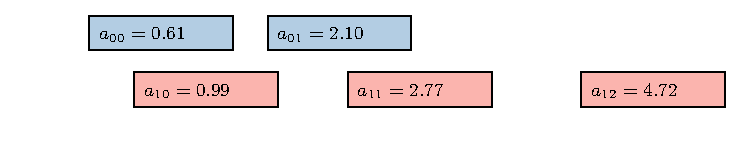
\includegraphics[scale=0.52]{../single/instance}
  \caption{Instance example with earliest arrival times indicated for each vehicle.}%
  \label{fig:instance-example}
\end{figure}

\begin{figure}[h]
  \centering
  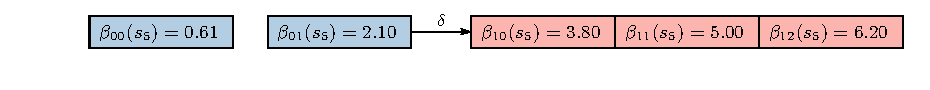
\includegraphics[width=0.98\textwidth]{../single/schedule}
  \caption{Some schedule as example solution to the problem instance shown in Figure~\ref{fig:instance-example}.}%
  \label{fig:solution-example}
\end{figure}


\section{Crossing time scheduling}\label{sec:crossing-time-scheduling}

The conclusion of the previous section is that, after making certain
assumptions, the trajectory optimization problem~\eqref{eq:single-trajectory-optimization} reduces to a scheduling
problem~\eqref{eq:C} of finding a schedule of crossing times $y$, determining the time at
which each vehicle in the system crosses the intersection.
%
Given such a schedule, corresponding trajectories can be computed relatively
efficiently for each route separately using a direct transcription method.
%
Hence, in the remainder of this chapter and the next chapter, the focus will be
on solving the crossing time scheduling problem.

This problem is inherently a combinatorial optimization problem, for which a
wealth of general solution techniques is
available~\cite{duIntroductionCombinatorialOptimization2022}, including
algorithms specifically tailored to problems that can be stated in terms of
finding optimal time
schedules~\cite{pinedoSchedulingTheoryAlgorithms2016,grahamOptimizationApproximationDeterministic1979}.
%
One of the most prominent distinction among such algorithms lies in whether it
guarantees to find an optimal solution or not.
%
Of course, it is desirable to find optimal solutions, but this is often not
tractable in practice, because the number of feasible solutions typically
explodes whenever larger instances are considered.
%
In other words: enumerating all solutions and evaluating their objective value
to find the best one is typically not achievable in any reasonable amount of
time.
%
This is the main motivation for the development of so-called heuristics, which
discard the optimality guarantee in favor of speed.

This thesis will illustrate both types of approaches.
%
In this section, we show how to leverage the general branch-and-cut framework by
formulating~\eqref{eq:C} as a mixed-integer linear
program and defining three types of cutting planes.
%
We conclude this section by an evaluation of the running time improvement of
these cutting planes. \comment{Clearly motivate why we want fast heuristics.}
%
The next chapter focuses mainly on heuristics and machine learning techniques to
tune heuristics to exploit specific structures often found in practical problem
instances.


\subsection{Integer programming as baseline}\label{sec:branch-and-bound}

% - first explain the general algorithmic branch-and-bound paradigm
% - then provide a brief general intro of MILP, pointing out its strengths and weaknesses

A very common algorithmic idea in combinatorial optimization is the
branch-and-bound strategy, in which the space of feasible solutions is
systematically explored using a search tree by iteratively subdividing the
feasible region into smaller subproblems (branching), computing bounds on the
best possible objective value within each subproblem (bounding), and discarding
those parts of the tree that contain subproblems whose bound proves them
incapable of containing an optimal solution (pruning).

A typical application of this scheme is found in algorithms for solving
mixed-integer programming problems.
%
In such problems, we optimize over $n$ real-valued decision variables $y_{i}$
for which possibly a subset $\mathcal{I} \subseteq \{1, \dots, n\}$ is
restricted to be integer-valued.
%
A canonical example of such problems is a mixed-integer linear program, where the
goal is to minimize
\begin{align}\label{eq:MILP}\tag{MILP}
  \min_{y} c^{T} y \text{ such that } Ay \leq b, \; y \in \mathbb{R}^{n}, \; y_{j} \in \mathbb{Z} \text{ for } j \in \mathcal{I},
\end{align}
given some matrix $A \in \mathbb{R}^{m\times n}$ and vectors
$b \in \mathbb{R}^{m}$ and $c \in \mathbb{R}^{n}$.
%
This surprisingly simple setup provides a powerful modeling toolkit to approach
many combinatorial optimization problems, because it allows discrete choices to
be modeled using integers.
%
We already saw an example of this when we applied the big-$M$ method in our
direct transcription of the trajectory optimization problem.

The branch-and-bound algorithm for~\eqref{eq:MILP} is based on progressively
constraining the integer decision variables as we move further from the root
node in the search tree.
%
At each node, the integer constraints are relaxed, producing a linear program
that can be solved efficiently.
%
The solutions of these relaxations provide the basis of the bounding step:
whenever the objective of the relaxation at some node is higher than that of the
currently best known feasible solution, the subtree at that node is pruned.

\paragraph{MILP reformulation.}

We show how to reformulate the crossing time scheduling
problem~\eqref{eq:C} into the form~\eqref{eq:MILP}. Note that we
only have to rewrite the disjunctive constraints~\eqref{eq:disjunctive}. For
each conflict $\{i,j\} \in \mathcal{D}$, this constraints essentially encodes
the crossing order of $i$ and $j$, i.e., whether $i$ crosses the intersection
before $j$, or vice versa.
%
We can rewrite these constraints using the big-$M$ method by introducing a
binary decision variable $\gamma_{ij}$ for every conflict $\{i, j\} \in \mathcal{D}$,
such that setting $\gamma_{ij} = 0$ corresponds to choosing the crossing order
$i \rightarrow j$ and $\gamma_{ij} = 1$ corresponds to $j \rightarrow i$.
%
To avoid redundant variables in a software implementation, it might be desirable
to induce some arbitrary ordering of the conflicting vehicles by defining the
index set
\begin{align}
  \bar{\mathcal{D}} = \{ (i,j) : \{i,j\} \in \mathcal{D}, \; r(i) < r(j) \} .
\end{align}
With this definition, we obtain the MILP reformulation
%
\begin{equation}\tag{C'}\label{eq:C'}
\renewcommand{\arraystretch}{1.2}
\begin{NiceArray}{ r l @{} >{{}}c<{{}} @{} l @{} }
  \displaystyle \min_{y,\gamma} & \displaystyle \sum_{i \in \mathcal{N}} y_{i} \\
  \text{s.t. } \; & a_{i} \leq y_{i} && \quad \text{ for all } i \in \mathcal{N} , \\
  & y_{i} + \rho \leq y_{j} && \quad \text{ for all } (i,j) \in \mathcal{C} , \\
  & y_{i} + \sigma \leq y_{j} + \gamma_{ij}M  &&  \\
  & y_{j} + \sigma \leq y_{i} + (1 - \gamma_{ij})M \hspace*{1.8em} && \quad \text{ for all } (i,j) \in \bar{\mathcal{D}} , \\
  & \gamma_{ij} \in \{0, 1\}
\CodeAfter\SubMatrix.{4-1}{6-2}\}
\end{NiceArray}
\end{equation}
%
where $M > 0$ is some sufficiently large number.

Note that this reformulating opens up the possibility to leverage the collective
effort that has gone into developing fast general solvers for this problem
class: many modern solvers, e.g., SCIP~\cite{BolusaniEtal2024OO} (academic) or
Gurobi~\cite{gurobi} (commercial), employ specialized interal heuristics and
techniques to derive better bounds and thus achieve more pruning of the search
tree to speed up the solving process.
%
Furthermore, a wide variety of software tooling is available. For example, we
used the AMPL modeling language to write the above formulation in a
solver-agnostic specification and use the
amplpy\footnote{\url{https://amplpy.ampl.com/}} package to call the solver from
the comfort of Python.

At the end of this section, we report some numerical results based on this
method. First, we show that the above formulation can be made a little sharper,
in some sense.

\subsection{Exploiting optimal substructure}

The branch-and-bound approach guarantees to find an optimal solution, but it
does not provide any guarantees on the required running time.
%
Roughly speaking, the running time depends mainly on two aspects: (i) size of
the instance---in our case: number of vehicles---and (ii) the amount of structure it
exhibits.
%
More specifically, the running time depends heavily on the efficiency of the
bounding step in pruning the search tree, which might vary wildly among
equivalent formulations.
%
A technique that is often used to make bounding more efficient is to add
so-called \emph{cutting planes}.
%
The basic idea is that we can introduce additional inequalities
without changing the set of feasible solutions
\begin{align}
  \{ y : Ay \leq b, A'y \leq b', y_j \in \mathbb{Z}, j \in \mathcal{I} \} = \{ y : Ay \leq b, y_j \in \mathbb{Z}, j \in \mathcal{I} \} ,
\end{align}
while achieving more efficient bounding.
%
There are general-purpose schemes for adding such cutting planes $A' y \leq b$,
but it often makes sense to also use insights into the specific problem at hand
to derive problem-specific cutting planes.
%
The branch-and-bound framework with cutting planes is colloqially referred to as
\emph{branch-and-cut}.

Next, we present insight into some optimal substructures of optimal solutions.
This analysis will serve as the basis for defining three types of cutting
planes.
%
Let us first consider some simple problem instances to start shaping our
intuition.

\begin{figure}
  \centering
  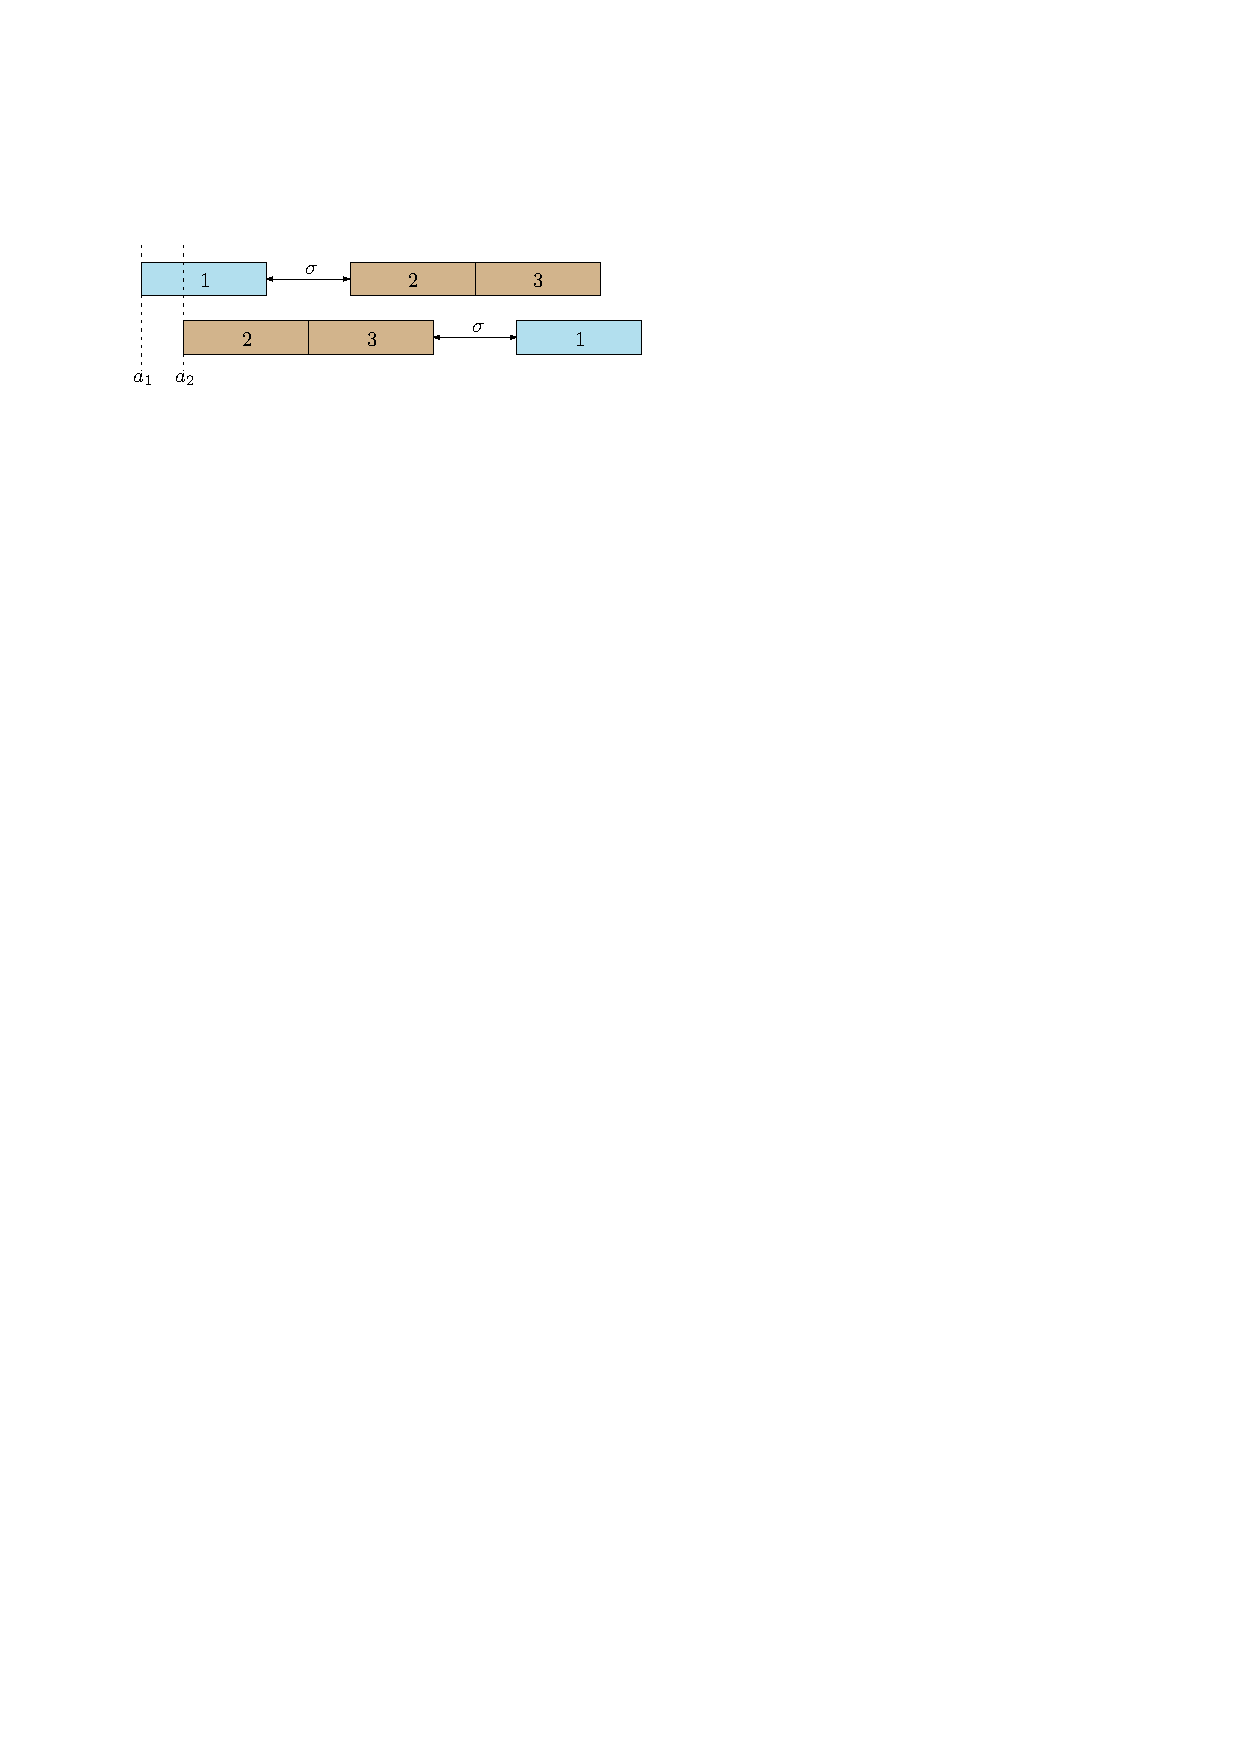
\includegraphics[width=0.55\textwidth]{figures/single/123.pdf}
  \caption{Illustration of the two possible sequences of vehicles in
    Example~\ref{example2}.}
  \label{fig:example2}
\end{figure}

\begin{eg}
  \label{example2}
  Consider two routes having one and two vehicles, respectively. Instead of
  $(1,1), (2,1), (2,2)$, we will use the labels $1, 2, 3$ to keep notation
  clear. We are interested in how the earliest crossing times $a_i$ influence the
  order of the vehicles in an optimal schedule. We set $a_{1} = 0$, without loss
  of generality, and assume that $a_{3} = a_{2} + \rho$. Suppose
  $a_{1} = a_{2}$, then we see that the order $2, 3, 1$ is optimal, which
  resembles some sort of ``longest chain first'' rule. Now suppose that
  $a_{1} < a_{2}$. For $a_{2} \geq a_{1} + \rho + \sigma$, the sequence
  $1, 2, 3$ is simply optimal. For $a_{2} < a_{1} + \rho + \sigma$, we compare
  the sequence $1, 2, 3$ with $2, 3, 1$, which are illustrated in
  Figure~\ref{fig:example2}. The first has
  $\sum_{i} y_{i} = (\rho+\sigma) + (\rho+\sigma+\rho) = 3\rho + 2\sigma$,
  while the second sequence has
  $\sum_{i} y_{i} = a_{2} + (a_{2} + \rho) + (a_{2} + \rho + \rho + \sigma) = 3 a_{2} + 3\rho + \sigma$.
  Therefore, we conclude that the second sequence is optimal if and only if
  \begin{align}
    \label{eq:before-condition}
    a_{2} \leq \sigma/3 ,
  \end{align}
  which roughly means that the ``longest chain first'' rule becomes optimal
  whenever the earliest crossing times are ``close enough''.
\end{eg}

In this example, we see that it does not make sense to schedule vehicle 1
between vehicles 2 and 3, because that would add unnecessary switch-over time
$\sigma$. This raises the natural question whether splitting such \textit{platoons} of
vehicles is ever necessary to achieve an optimal schedule. To answer this
question, let us first give a precise definition of platoons, before slightly
generalizing the example.
%
\begin{define}
  A sequence of consecutive vehicles $(r, l+1), (r, l+2), \dots, (r, l+n)$ from
  some route $r$ is called a \textit{platoon} of size $n$ if and only if
  \begin{align}
  a_{(r,k)} + \rho = a_{(r, k+1)}  \quad \quad \text{ for all } l < k < l + n.
  \end{align}
 We say that the platoon is \textit{split}
  in some schedule $y$, if
  \begin{align}
  y_{(r, k)} + \rho < y_{(r, k + 1)} \quad \quad \text{ for some } l < k < l + n.
  \end{align}
\end{define}
%
\begin{eg}
  \label{example3}
  Suppose we have two routes $\mathcal{R} = \{ A, B \}$, each having exactly one
  platoon, denoted as $P_{A} = ((A,1), \dots, (A,n_{A}))$,
  $P_{B} = ((B,1), \dots, (B,n_{B}))$. To simplify notation, we write
  $a_{A} = a_{(A,1)}$ and $a_{B} = a_{(B,1)}$. We assume $a_{A} = 0$, without
  loss of generality, and suppose that $n_{A} < n_{B}$ and
  $a_{A} \leq a_{B} < n_{A}\rho + \sigma$. Consider the ways the two platoons
  can merge by splitting A. Let $k$ denote the number of vehicles of platoon A
  that go before platoon B and let $\sum y_{i}(k)$ denote the corresponding
  sum of crossing times. See Figure~\ref{fig:example3} for an illustration of the
  situation in case of $a_{A} = a_{B}$. For $0 < k \leq n_{A}$, we have
  \begin{align*}
    \sum_{i \in \mathcal{N}} y_{i} (k) = \max\{ \sigma, a_{B} - k\rho\} (n_{B} + n_{A} - k) + \sigma (n_{A} - k) + \sum_{j=1}^{n_{A}+n_{B}} (j-1) \rho ,
  \end{align*}
  so when platoon A goes completely before platoon B, we get
  \begin{align*}
    \sum_{i \in \mathcal{N}} y_{i} (n_{A}) = \sigma n_{B} + \sum_{j=1}^{n_{A}+n_{B}} (j-1) \rho ,
    \label{eq:A-before-B}
  \end{align*}
  since $\max\{ \sigma, a_{B} - n_{A} \rho \} = \sigma$ by the assumption on $a_{B}$. It is
  easily seen that we have $\sum y_{i}(k) > \sum y_{i} (n_{A})$ for $0 < k < n_{A}$,
  so in other words, if we decide to put at least one vehicle of platoon A
  before platoon B, it is always better to put all of them in front. As we will
  see after this example, this principle holds more generally.

  For $k=0$, so when we schedule platoon A completely after platoon B, the total
  completion time becomes
  \begin{align*}
    \sum_{i \in \mathcal{N}} y_{i} (0) = a_{B} (n_{A} + n_{B}) + \sigma n_{A} + \sum_{j=1}^{n_{A}+n_{B}} (j-1) .
  \end{align*}
  Comparing this to~\eqref{eq:A-before-B}, we conclude that placing B in front
  is optimal whenever
  \begin{align*}
    a_{B} \leq (n_{B} - n_{A}) \sigma / (n_{A} + n_{B}) ,
  \end{align*}
  which directly generalizes the condition~\eqref{eq:before-condition} that we
  derived for the case with $n_{A} = 1$ and $n_{B} = 2$. (end of example)
\end{eg}

\begin{figure}
  \centering
  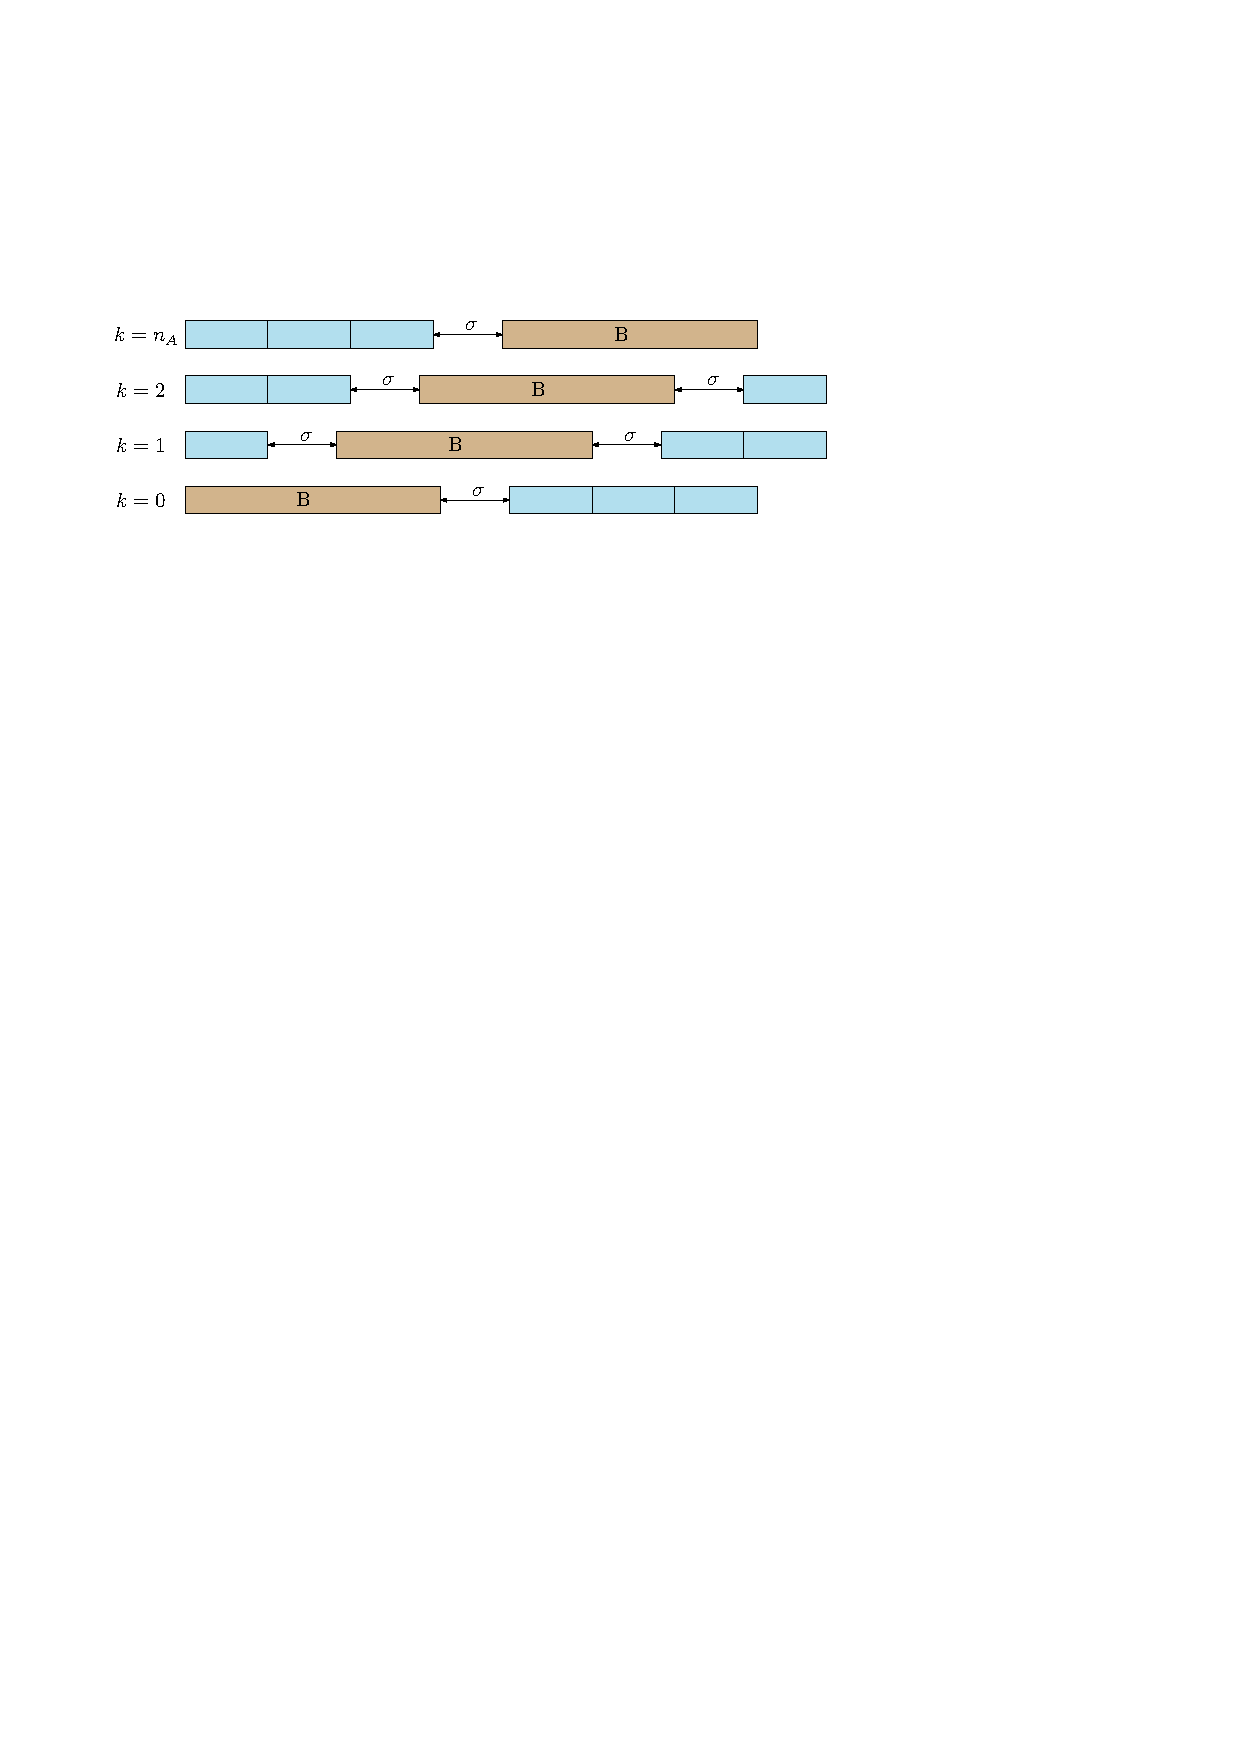
\includegraphics[scale=0.9]{figures/single/platoons.pdf}
  \caption{Different ways to split platoon A, regarding Example~\ref{example3}, assuming
    equal earliest crossing times $a_{A} = a_{B}$ with $n_{A} = 3$ vehicles in
    platoon A and some arbitrary number of vehicles $n_{B}$ in platoon B.}
  \label{fig:example3}
\end{figure}

The example shows that, when we decide to put one vehicle of a platoon before
another platoon, it is always better to put all vehicles of the platoon in
front. In other words, whenever a vehicle can be scheduled immediately after its
predecessor, this should happen in any optimal schedule. It turns out that this
property holds more generally, as stated by the following result. \comment{[add
  proof in Appendix]}

\begin{restatable}[Platoon Preservation~\cite{limpensOnlinePlatoonForming2023}]{theorem}{Exhaustive}\label{thm:exhaustive}
  If $y$ is an optimal schedule for~\eqref{eq:C},
  satisfying $y_{i^{*}} + \rho \geq a_{j^{*}}$ for some $(i^{*},j^{*}) \in \mathcal{C}$, then $j^{*}$
  follows immediately after $i^{*}$, so $y_{i^{*}} + \rho = y_{j^{*}}$.
\end{restatable}

\paragraph{Cutting planes.}
Based on the above analysis of optimal substructure, we will define three types
of cutting planes for~\eqref{eq:C'}.
%
First, we will use Theorem~\ref{thm:exhaustive} to formulate two types of
cutting planes. The idea is that we try to model this necessary condition for
optimality within the MILP formulation. To do so, we introduce a binary variable
$\delta_{ij} \in \{0, 1\}$, for every conjunctive pair $(i,j) \in \mathcal{C}$, which we
want to satisfy
\begin{align*}
  \delta_{ij} = 0 &\iff y_{i} + \rho < a_{j} , \\
  \delta_{ij} = 1 &\iff y_{i} + \rho = a_{j} .
\end{align*}
Again, this can be enforced using the big-$M$ method, by adding the constraints
\begin{subequations}
\begin{align}
  y_{i} + \rho &< a_{j} + \delta_{ij}M ,  \\
  y_{i} + \rho &\geq a_{j} - (1 - \delta_{ij}) M .
\end{align}
\end{subequations}
Now observe that the statement of Theorem~\ref{thm:exhaustive} applied to $(i,j)$ is equivalent
to the inequality
\begin{align}
  y_{i} + \rho &\geq y_{j} - (1 - \delta_{ij}) M \tag{conj.cut} .
\end{align}
We refer to these cutting planes as \textit{necessary conjunctive cutting planes}.

Using the definition of $\delta_{ij}$, we can derive one more type of cutting planes
on the disjunctive decision variables $\gamma$. Whenever $\delta_{ij} = 1$,
Theorem~\ref{thm:exhaustive} implies that we have $i \rightarrow k$ and $j \rightarrow k$ for every
other vehicle $k \in \mathcal{N}$ on a different route $r(k) \neq r(i) = r(j)$,
which can be enforced by adding the constraints
\begin{subequations}
\begin{align}
  \delta_{ij} + (1 - \gamma_{ik}) + \gamma_{jk} \leq 2 , \tag{disj.cut.1} \\
  \delta_{ij} + \gamma_{ik} + (1 - \gamma_{jk}) \leq 2 . \tag{disj.cut.2}
\end{align}
\end{subequations}
We will refer to these as the \textit{necessary disjunctive cutting planes}.

The last type of cutting plane is related to some kind of redundancy in the
encoding of feasible crossing orders.
%
Observe that the constraints $y_i + \rho \leq y_j$ cause a fixed order of
crossing for all vehicles on the same routes. Hence, let $\mathit{pred}(i)$
denote the set of all vehicles on route $r(i)$ that cross the intersection
strictly before vehicle $i$ and let $\mathit{succ}(i)$ denote those that cross
strictly later,
%
\comment{Alternatively, we could say these are all the vehicles from which there is a path of conjunctive arcs to $i$, but then we would have to introduce the disjunctive graph.}
%
so we have
\begin{align*}
  \mathit{pred}(i) := \{ (r(i), k) : k > k(i) \} , \\
  \mathit{succ}(i) := \{ (r(i), k) : k < k(i) \} .
\end{align*}
%
Suppose we have some solution $(y,\gamma)$ that satisfies $\gamma_{ij} = 0$ for
some conflict pair $(i,j) \in \bar{\mathcal{D}}$, so $i \rightarrow j$, then it is
clear that $\gamma$ must also satisfy
\begin{align*}
  \gamma_{pq} = 0 \quad (\text{so } p \rightarrow q) \quad \text{ for all } \, p \in \mathit{pred}(i), \, q \in \mathit{succ}(j) .
\end{align*}
Using the big-$M$ method, we can equivalently encode this as
\begin{align}
  \sum_{\substack{p \in \mathit{pred}(i)\\ q \in \mathit{succ}(j)}} \gamma_{pq} \leq \gamma_{ij} M . \tag{trans.cut}
\end{align}
Every feasible $(y,\gamma)$ must satisfy the above inequality for every
$(i,j) \in \bar{\mathcal{D}}$, so we can safely add them to~\eqref{eq:C'}
without changing the problem. We refer to these inequalities as the
\emph{transitive cutting planes}.

\paragraph{Runtime benchmark.}

We conclude this section with an evaluation of the running time of the
branch-and-bound approach.
%
Since the running time is primarily determined by the total number of vehicles
in the system, we consider problem instances with two routes and report
running times as a function of the number of vehicles per route.
%
Problem instances are generated with fixed processing time $\rho=4$, switch-over
time $\sigma=1$, and randomly generated earliest crossing times $a_i$.
%
A detailed discussion of the distribution of $a_i$ that we used is deferred to
the end of the next chapter, where a more extensive comparison will be provided.

\note{To illustrate the benefit of each proposed cutting plane, we also include
results for the case without any cutting planes.}
%
To keep the total computational effort within reasonable limits, we impose a
time limit of 60 seconds per instance.
%
Consequently, some care must be taken when interpreting the average running
time, because some observations correspond to cases in which the algorithm
reaches the time limit.\footnote{In statistics, such observations are called \emph{censored}
  and there are generally better ways of handling these. However, we do not need
  such rigorous analysis for the argument here.} For this benchmark, we used
the Gurobi solver version 11.0.2 on a system with a 13th Gen Intel i5-13600K CPU
and 32GiB of RAM.
%
Figure~\ref{fig:running_time} shows the average running time for the three types of cutting planes.
Observe that the necessary conjunctive cutting planes provide the most
significant runtime improvement.

\begin{figure}
  \centering
  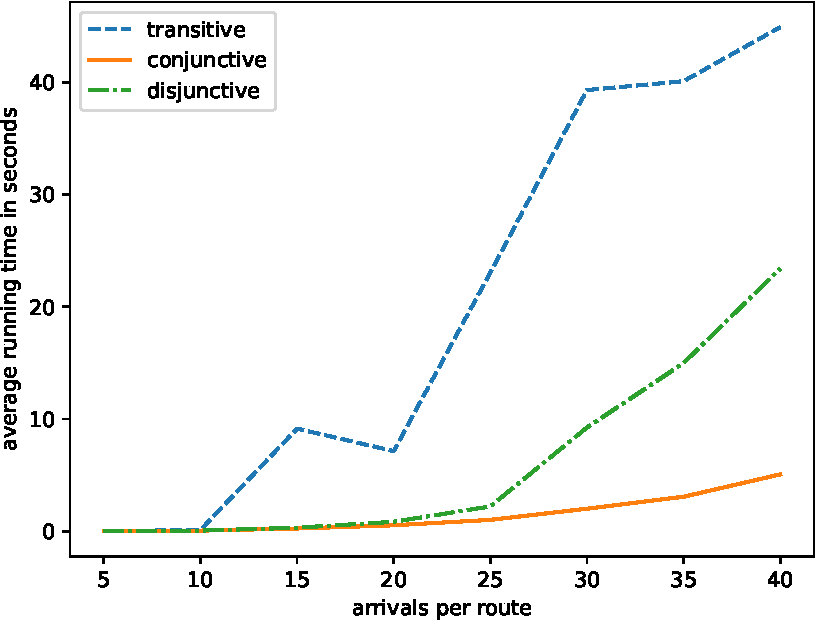
\includegraphics[width=0.8\textwidth]{data-single/running_times.pdf}
  \caption{\note{[current figure is placeholder]} The average running time of
    the branch-and-cut procedure is plotted as a function of the number of
    arriving vehicles per route, for each of the three indicated cutting planes.
    Each average is computed over $20$ problem instances. All instances use
    $\rho = 4$ and $\sigma = 1$. The earliest crossing times for vehicles are generated
    using the bimodal exponential interarrival time model from
    Section~\ref{sec:results} with parameters $p=0.5, \mu_{s} = 0.1, \mu_{l} = 10$.
    This figure clearly shows that the conjunctive cutting planes provide the
    most runtime improvement. \comment{Why not show the case without any cutting
      planes? Because this takes sooo much time. What we could do is give some
      idea of this for up to 10 arrivals per route.}}
  \label{fig:running_time}
\end{figure}


\section{Notes and references}

The single intersection model is mostly based on the model described in the PhD
thesis of Hult~\cite[Chapter 3]{hultOptimizationBasedCoordination2019}.
%
Due to the simple rectangular geometry of the vehicles and the fact that routes
are straight, it is easy to compute the conflict area in configuration space,
for which we provide details in Appendix~\ref{app:configuration-space}. For
general curved trajectories, the computation is more involved, see for
example~\cite[Appendix A]{levinConflictpointFormulationIntersection2017}
and~\cite[Section 2.2]{liTemporalspatialDimensionExtensionbased2019}.

The bilevel decomposition and approximation scheme of Section~\ref{sec:bilevel}
are further detailed in~\cite{hultApproximateSolutionOptimal2015,hultTechnicalReportApproximate}.
%
In proving that the decomposed problem is equivalent to the original trajectory
optimization problem, they state that the lower-level problem has a unique
solution. We emphasize that this depends on \emph{strict} convexity of the objective function.
%
For the problem without state constraints, this has been rigorously proven in~\cite[Theorem 5.1, part
(V)]{hanUnifiedNumericalScheme2012}, where uniqueness indeed depends on the positive
definiteness of the matrix $R$ defining the quadratic component $u^T R u$ of the
running cost function with respect to the control variable.

At various points in this chapter, we included some comments from the optimal
control perspective. For a textbook introduction of optimal control theory, we
recommend the book of Liberzon~\cite{liberzonCalculusVariationsOptimal}. The focal point in their presentation is the
Pontryagin maximum principle, which provides neccessary conditions for
optimality for optimal control problems.
%
When dealing with state-constrained problems, the most relevant overview of
results we could find is the survey of Hartl et al.~\cite{hartlSurveyMaximumPrinciples1995}.
%
We note that, although the theory for dealing with state constraints (\`a la
Pontryagin) is far from complete, in practice, they can be successfully dealt
with in numerical approaches, often involving some sort of penalty function.

A solid introduction to the algorithmic foundations for integer programming is
provided by the book~\cite{confortiIntegerProgramming2014}, whose introductory chapter also contains a clear
description of the branch-and-cut methodology. For an introduction of integer
programming with a focus on solving scheduling problems, we like to refer
to~\cite[Appendix A]{pinedoSchedulingTheoryAlgorithms2016}.
%
Note that decomposition techniques similar in nature to the decomposition of
Section~\ref{sec:bilevel} have a relatively long history in mathematical programming.
Well-known examples in the context of mixed-integer linear programming include
Dantzig-Wolfe decomposition and Benders' decomposition.\footnote{Fun fact: this
  famous method is named after Jacques
  Benders~\cite{aardalJacquesBendersHis2025}, who was a professor here at \TUE.}
%
Such techniques have been applied in air traffic scheduling~\cite{manninoPathCycleFormulation2018} and job-shop
problems arising in general traffic scheduling problems~\cite{lamorgeseNoncompactFormulationJobShop2019}.
%
Interestingly, these works also propose an alternative (``noncompact'') MILP
formulation that does not depend on the big-$M$ trick. From our current limited
understanding, this seems to be related to, and might be a better alternative to
our ``transitive cutting planes''.


\chapter{Learning to schedule}\label{chap:single-learning}

% sequence modeling
Most methods that are based on some kind of branch-and-bound tree search are
guaranteed to find an optimal solution, but as we illustrated with our benchmark
in Section~\ref{sec:crossing-time-scheduling}, without further modifications, the running time still scales
very poorly with increased instance sizes.
%
Once we start considering multiple intersections, this scaling issue is expected
to become even more prominent, so we first try to obtain fast algorithms for the
single intersection crossing time scheduling problem with large numbers of
vehicles, thereby sacrificing optimality guarantees in favor of speed and
potential for scalability.
%
Specifically, in this chapter, we are interested in developing heuristics to
obtain good schedules, with close to optimal total travel delay, in limited
time.

% outline
Before we discuss our methodology for solving the crossing time scheduling
problem~\eqref{eq:C}, Section~\ref{sec:ml-co} first
provides some background on the general idea of leveraging machine learning
techniques to solve combinatorial problems.
%
We introduce the central idea of treating problem instances and solutions as
training data points and mention some key works to illustrate the general
methodology.

% our methodology
Our own machine learning approach hinges on the ability to encode candidate
solutions for the crossing time scheduling
problem~\eqref{eq:C} as a sequence of route indices,
which is discussed in Section~\ref{sec:sequence-representation}.
%
The idea is that we only have to decide in which order vehicles are able to
cross the intersection, and since the relative route of vehicles on the same
route is already fixed, this leaves us with ordering the routes.
%
It is straightforward to show that the corresponding crossing times, given this
crossing order, follow as the solution to a linear program.
%
Additionally, we show that partial solutions provide a certain lower bound on
the crossing times.

\emph{The problem is reduced to a sequence learning problem.}

Next, we show in Section~\ref{sec:seq-modeling} how to construct a probabilistic
sequence model over schedules, by assigning a conditional probability to every
candidate solution sequence, conditional on the problem instance.
%
We propose two different parameterizations of the model.
%
One parameterization is based on the Platoon Preservation
Theorem~\ref{thm:exhaustive}. The other is based on a recurrent neural network
encoding of the crossing time lower bounds.

We show how to use randomly generated problem instances to fit the model
parameters.
%
There are generally two main approaches here. The most straightforward way is to
use an existing solver to compute optimal solutions, then use these as training
data points in a supervised learning setting.
%
However, this assumes that we are able to solve the combinatorial problem in the
first place.
%
An alternative approach is to try to learn how to construct such optimal
sequences by trial-and-error, by evaluating the current model to determine the
next route in the sequence, and then updating the model parameters based on an
intermediate score, which is best understood in the framework of reinforcement
learning.

\clearpage

\section{Machine learning for combinatorial optimization}\label{sec:ml-co}

Recent years have seen increased research interest in using models and methods
from the machine learning (ML) community for solving combinatorial optimization
problems (CO).
%
In this section, we first discuss some key ideas and techniques found within
this line of work.
%
Based on this, we give an overview of our methodology for solving the crossing
time problem.

\subsection{Context and motivation}

In typical CO problems, we try to find some the best option from some set of
discrete structures such as graphs, sets, sequences, etc.
%
Typical problems involve, for example, finding some path or route through a
graph, like in the traveling salesman problem; selecting some optimal subset,
like in the knapsack problem or set cover problem; or selecting the best
sequence in which machines are assigned to pending jobs, as in job-shop
scheduling.
%
Generally speaking, we can think of CO problems as being concerned with finding
an optimal configuration vector $v \in V$ from a finite\footnote{This assumption
  simplifies our current discussion, but note that some typical combinatorial
  problems have infinitely many feasible solutions.
%
  It is not trivial to distinguish between \emph{continuous} optimization
  and \emph{combinatorial} optimization.
%
  We could call a problem combinatorial if at least one component $v_i$ of the
  configuration $v \in \mathbb{R}^n$ is restricted to lie in some countable domain.
%
  For example, this is the case for mixed-integer programs, where some
  variables are restriced to the integers.
%
  However, some problems that should be called continuous according to this
  definition are more combinatorial in nature than it seems at first sight. For
  example, the feasible set of a linear program is generally not a finite set,
  but Dantzig's simplex algorithm shows that the optimal solution must be one of
  the finitely many vertices of the convex polytope.} set of candidates, such
that some objective function $f : V \rightarrow \mathbb{R}$ is minimized.
%
Since there are only finitely many candidates, a straightforward solution is to
just evaluate the objective for each candidates $v \in V$ and then output some
configuration for which $f(v)$ is minimal.
%
However, for all but trivial problems, this is simply not feasible in any
reasonable amount of time, which is the central motivation in the field of
combinatorial optimization.

In almost all practically relevant CO problems, the \emph{objective} function
$f$ exhibits some kind of regularity.
%
Therefore, when developing algorithms, a good strategy is to look for such
structure in the problem that can be exploited algorithmically.
%
% proofs -> algorithmic ideas with optimality guarantees
Such structural insights can be precise, like in Theorem~\ref{thm:exhaustive}, and methods like
those based on the branch-and-bound scheme try to take advantage of such
well-defined structure. Often, such algorithms come with some kind of guarantee
on the quality of the returned solution.
%
% intuition -> algorithmic ideas without guarantees
Other algorithms are based on some hard-to-define intuition about what optimal
solutions should look like.
%
This very much applies to so-called \emph{local search} algorithms.

\paragraph{Literature overview.}
Within this context, two main motivations for applying ML for solving CO
problems can be identified in the current
literature~\cite{bengioMachineLearningCombinatorial2020}, which we discuss next.
%
The key publications on which the following discussion is based are collected in
Table~\ref{tab:ml-co-literature}.

\emph{1. Fast approximations.}
%
We might want to replace certain expensive computations of an existing
algorithms such as branch-and-bound with fast ML approximations.
%
Please note that the approximate nature of ML models does not necessarily impact
optimality guarantees of the original algorithm.
%
This is clearly illustrated by~\cite{gasseExactCombinatorialOptimization2019}, where the branching decision in
branch-and-bound is approximated, and the line of work related to~\cite{tangReinforcementLearningInteger2020}, where
ML models are employed for cutting plane selection.
%
In both examples, the algorithm is still guaranteed to obtain an optimal
solution, as long as the model provides valid branching decisions or valid
cutting planes.
%
Schemes in which ML models are integrated within some existing CO algorithm have
been referred to as \emph{joint} methods.

\emph{2. Algorithm discovery.}
%
Instead of trying to improve existing algorithms, we could try to employ ML to
explore the space of algorithms to find new, hopefully better, algorithms.
%
This type of approaches can also be understood as constructing a solution from
scratch or in terms of predicting the optimal solution, given the problem
instance.
%
Our method, that we will propose in Section~\ref{sec:seq-modeling}, belongs to this class of
so-called \emph{principal} methods.

\paragraph{Central ideas.}
In both cases, the premise is that \emph{ML can be used to discover certain
  regularities of the problem automatically}.
%
Therefore, one of the central ideas is to treat problem instances and their
solutions and training data for a machine learning model~\cite{bengioMachineLearningCombinatorial2020}.
%
This training data is used to fit a machine learning model and the hope is that
it somehow captures model structure similar to our intuition.
%
In the next subsection, we will make this notion more precise by presenting
the process of designing algorithms for CO problems as an optimization problem
in and of itself.
%
After that, we show how to state this in terms policy optimization in some
Markov decision process (MDP), opening up the application of optimization
methods from reinforcement learning.

\newcolumntype{L}[1]{>{\RaggedRight\hsize=#1\hsize\hspace{0pt}}X}
\begin{table}
\centering
\renewcommand{\arraystretch}{1.2}

\begin{adjustbox}{center}
\scalebox{0.8}{
\begin{tabularx}{1.4\textwidth}{@{} l L{0.5} L{1.5} @{}}
\toprule
\textbf{Reference} &
\textbf{Problem focus} &
\textbf{Contribution / Method} \\
\midrule
\citet{bengioMachineLearningCombinatorial2020} & General CO problems & Survey on using ML for CO, framing the learning problem \\
\citet{mazyavkinaReinforcementLearningCombinatorial2020} & General CO problems & Survey on using ML for CO, with a focus on reinforcement learning \\
\citet{daiLearningCombinatorialOptimization2018} & Graph problems & Deep RL with graph embeddings to construct solutions \\
\citet{vinyalsPointerNetworks2017a} & TSP & Pointer networks for sequence-based combinatorial problems \\
\citet{koolAttentionLearnSolve2019} & Routing problems & Attention model trained with RL for solving TSP, VRP \\
\citet{gasseExactCombinatorialOptimization2019} & MILP & Approximate strong branching policy with GNNs in branch-and-bound \\
\citet{tangReinforcementLearningInteger2020} & ILP & Attention-based model for cutting plane selection trained with RL \\
\citet{gravesNeuralTuringMachines2014} & General computation & Neural turing machine as a differentiable model of universal computation \\
\bottomrule
\end{tabularx}}
\end{adjustbox}
\caption{Some key references on machine learning for combinatorial optimization.}%
\label{tab:ml-co-literature}
\end{table}


\subsection{Algorithm development as optimization problem}

% The process of designing an algorithm itself may be considered as an
% optimization problem.
%
Let $s = (V, f) \in \mathcal{I}$ denote some particular instance of a
combinatorial problem and let $\pi \in \Pi$ denote some set of possible
algorithm for solving it---we will make the definition of $\Pi$ more precise
later.
%
Let $m : \mathcal{I} \times \Pi \rightarrow \mathbb{R}$ denote some function
that measures the performance of executing algorithm $\pi$ on problem instance
$s$. Function $m$ may involve aspects like whether the algorithm actually finds
a valid solution, optimality of the found solution, running time and usage of
other resources like memory, etc.
%
Using this notation, the goal of the algorithm developer can be succintly
formulated as
\begin{align}
  \min_{\pi \in \Pi} m(s, \pi) .
\end{align}
However, this single-instance situation is not very typical. More often we have
some class of instances $\mathcal{I}$ of interest, say, the set of all traveling
salesman problems.
%
Let $m(s, \pi)$ measure the running time of the algorithm, then from the
perspective of the classical worst-case running time analysis, the algorithm
developer's goal is now
\begin{align}
  \label{eq:min-max-runtime}
  \min_{\pi \in \Pi} \max_{s \in \mathcal{I}} m(s, \pi) .
\end{align}

\paragraph{Problem distribution.}

In principle, we wish to devise algorithms that perform as good as possible for
all possible instances $\mathcal{I}$. However, in most practical application, we
are only dealing with a narrow subset of $\mathcal{I}$, often consiting of very
similar problems.
%
To model the relative occurence and/or importance of problems, we can induce a
probability distribution $P$ over $\mathcal{I}$.
%
To illustrate this, imagine some delivery company in Eindhoven that needs to
solve many instances of the vehicle routing problem (VRP) every
day~\cite{bengioMachineLearningCombinatorial2020}. The problems they encounter
are often similar in some sense: many customers are located in the north, with
only a few regular customers at the \TUE campus; it often turns out to be
beneficial to plan routes that use the ring road, etc. The company does not care
about solving all possible VRPs, just their particular kind. This example is
further illustrated in Figure~\ref{fig:problem-distribution}.

There is some underlying, but unknown, probability distribution $P$ describing the
instances the company will likely face.
%
This distribution captures the problem instances the company actually cares
about.
%
Hence, instead of~\eqref{eq:min-max-runtime}, the company is actually more
interested in\comment{It can be argued that this ``sharper'' objective
  is even necessary in some sense due to the no free lunch theorem.}
\begin{align}
  \label{eq:max-expected-performance}
  \min_{\pi \in \Pi} \mathbb{E}_{s \sim P} \left[ m(s, \pi) \right] .
\end{align}
%
However, since $P$ is generally inaccessible, we need to resort to using
samples, which could be obtained from historical company data, for example.
%
Suppose that we have some set of training instances $D_\text{train} \sim P$ at
our disposal, then we could approximate~\eqref{eq:max-expected-performance} by solving
\begin{align}
  \min_{\pi \in \Pi} \sum_{s \in D_\text{train}} \frac{1}{|D_\text{train}|} m(s, \pi) .
\end{align}


\begin{figure}
  \centering
  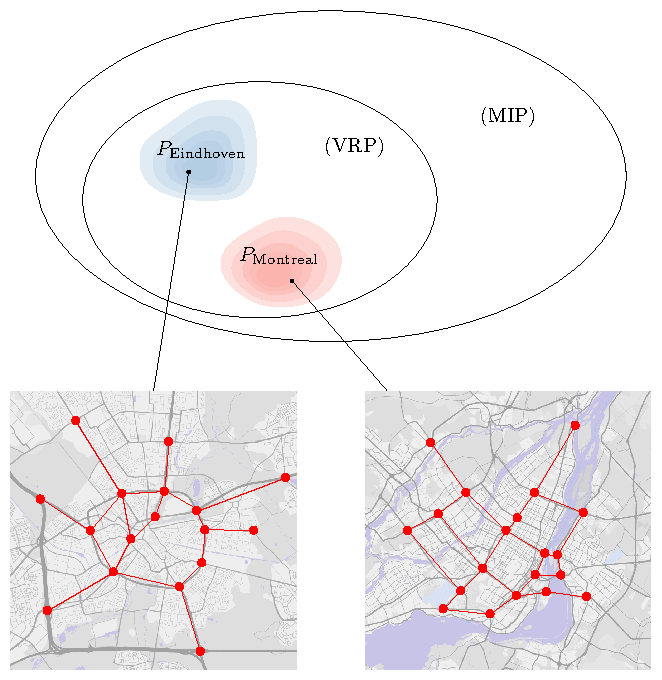
\includegraphics[scale=1]{figures/problem-distribution.pdf}
  \caption{Illustrating distributions of problems.
    %
    The top of the figure illustrates a typical hierarchical relationship between classes
    of combinatorial problems: instances of the vehicle routing problem (VRP)
    can be understood as specific instances of mixed-integer programs (MIP) and this relationship is mathematically well-defined.
    %
    In contrast to this clear boundary between problems, it might make more
    sense to consider a less sharp boundary between classes of problems by
    considering their distribution instead.
    %
    For example, we might consider the distribution $P_\mathrm{Eindhoven}$ of
    VRPs encountered by some delivery company in Eindhoven. The left graph
    illustrates a typical sample from this distribution.
    %
    Suppose this delivery company also has a branch in Montreal, then the distribution $P_\mathrm{Montreal}$ of problems faced by that branch will be very different.
    %
    For example, the Dommel river does not have such a large influence on the
    connectivity in Eindhoven compared to that of the St. Lawrence River.
    Furthermore, Eindhoven has some sort of circular connectivity due to the
    ring road, whereas large parts of Montreal are fairly Manhattan-like. It
    should be clear that statements like these are very cumbersome to formalize
    precisely, which is one of the main motivations of the ML for CO
    methodology.}\label{fig:problem-distribution}
\end{figure}


\paragraph{Class of algorithms $\Pi$.}
To make the algorithm optimization idea outlined above more concrete, we first
need to fix a suitable representation for the set of algorithms $\Pi$. In
principle, we could take $\Pi$ to consist of all possible C programs, or all
Python programs, for example. However, real-world code runs on a complex stack
of compilers, interpreters, and other complicating factors like hardware
optimizations. Therefore, it might be more desirable to work with simplified
models of computation. A common modeling choice in the ML for CO literature is
to represent algorithms as policies for Markov decision processes (MDPs). This
perspective naturally connects algorithm optimization to reinforcement learning
methods, which many existing works indeed
leverage~\cite{mazyavkinaReinforcementLearningCombinatorial2020,daiLearningCombinatorialOptimization2018,koolAttentionLearnSolve2019}.
In what follows, we show how the MDP framework arises naturally as a model of
computation and explain why it provides a particularly useful abstraction within
the contex of algorithm optimization.

\subsection{MDP as model of computation}

% DFA = base model
A key idea in the existing ML for CO literature is to model the class of
candidate algorithms in terms of policies for some Markov decision process
(MDP).

\paragraph{Finite-state automaton.}
First, we show how the execution of an algorithm can be viewed as a particular
state transition sequence of some deterministc finite-state automaton (DFA). Let
$\mathcal{S}$ be the finite set of states, with
$\mathcal{S}_0 \subseteq \mathcal{S}$ denoting the initial states, encoding
problem instances, and $\mathcal{S}_f \subseteq \mathcal{S}$ denoting the final
states that represent possible outputs. The remaining states capture the
\emph{internal state} of the algorithm, consisting of all relevant data
structures in memory.
%
Let $\mathcal{A}$ denote the finite non-empty set of
\emph{actions}\footnote{Note that ``input alphabet'' is actually more common
  terminology for DFAs, because of their origins in complexity theory and formal
  languages, where they are said to \emph{accept} or \emph{reject} a certain
  sequence of input symbols depending on the final state. In some sense, they
  are strictly less powerful than Turing machines, the latter being regarded as
  the most powerful/complete model of computation (Church-Turing thesis).}
%
and let $p : \mathcal{S} \times \mathcal{A} \to \mathcal{S}$ be some
\emph{transition function} that specifies the next state when a particular
action is chosen.
%
In this context, an algorithm can be viewed as a \emph{policy} function
$\pi : \mathcal{S} \rightarrow \mathcal{A}$ that provides the action to be taken
from each state.
%
The policy parameterizes the automaton’s execution similar to how program code
determines the state transitions of a computer.
%
% performance measure
In this model, the performance of running algorithm $\pi$ on instance $s$ is
measured\footnote{To accomodate this, states may need to carry auxiliary
  meta-information such as total number of transitions or bounds on the quality
  of the solution. Actual running time is not captured by this simple model
  formulation, but the number of transitions can be used as a proxy. This is no
  immediate problem: the current model is merely used as a way of introducing
  the general methodology.} in terms of the unique final state $s_f^\pi$ by some
cost function $c : \mathcal{S}_f \rightarrow \mathbb{R}$, such that we have
$m(s,\pi) = c(s_f^\pi)$.

% optimization and restriction of $\Pi$ through choice of $\mathcal{S}$
\paragraph{Designing the automaton.}

With this model in hand, we can now define $\Pi$ to be the set of valid policy
functions for some fixed automaton.
%
Hence, the automaton definition becomes a key decision in the algorithm
optimization, because fixing a particular state space effectively restricts the
class of algorithms.
%
The algorithm designer can choose to use a very general automaton, similar to a
Turing machine, or incorporate prior knowledge and intuition by carefully
defining a more restricted state space.
% example: local search
To illustrate this, suppose we let the state space represent all possible
permutations of nodes in a traveling salesman problem, then $\Pi$ would
naturally model all possible local search algorithms.
%
Indeed, any permutation of the nodes corresponds to a valid tour such that any
state is a valid solution, so we have $\mathcal{S}_f = \mathcal{S}$.
%
The transition function $p$ implicitly defines the \emph{neighborhood} of each
solution, and the policy $\pi$ specifies which neighbor to choose, capturing the
essence of the local search process.

% towards MDP
\paragraph{Markov decision process.}
We can generalize the automaton defined above as follows.
% stochastic transitions
% stochastic policy
Instead of a single next state, the transition function $p$ becomes a mapping to
distributions of states.
similarly, we let policies map to distribution over actions.
Therefore, we now write
\begin{align*}
  p : \mathcal{S} \times \mathcal{A} \rightarrow \Delta(\mathcal{S}) \quad \text{ and }
  \quad \pi : \mathcal{S} \rightarrow \Delta(\mathcal{A}) .
\end{align*}
%
This generalization turns the automaton into a finite-horizon MDP, with $r = {-c}$
taking the role of final reward function.
%
To take into account the additional stochasticity this introduces, we can generalize the algorithm development objective~\eqref{eq:max-expected-performance} to
\begin{align}\label{eq:max-mdp-performance}
  \max_{\pi \in \Pi} \mathbb{E}_{s \sim P} \left[ \, \mathbb{E}_\pi \left[ r(s_f^\pi) \mid s \right] \, \right] ,
\end{align}
where the inner expectation corresponds to the randomness of policy evaluation
in the MDP, because $s_f^\pi$ is now a random variable, and $\Pi$ still denotes
the set of all \textbf{deterministic} policies.

% stochastic transitions
\paragraph{Why is stochasticity useful?}
It might not be immediately clear why we would want to introduce stochasticiy in
a seemingly deterministic problem environment.
%
We will discuss two reasons why the MDP framework is nevertheless an attractive
starting point.
\comment{These reasons are also loosely tied to the the two main motivations introduced
at the beginning of this section, which were ``fast approximations'' and
``algorithm discovery''.}

First of all, non-deterministic transitions can be used to model certain parts
of the computation that are too complex to model explicitly.
%
This has for example been done in previouw joint methods, in which some part of
an existing CO solver is augmented by replacing a specific component with a ML
model.
%
For example, we might take some existing integer programming solver as the base
algorithm, while parameterizing a specific component, say, cutting plane
selection, as done in~\cite{tangReinforcementLearningInteger2020}.
%
In that case, the actions $\mathcal{A}$ correspond to selecting some valid
cutting plane, upon which the state transition $p$ models the whole of the
execution of the solver until the next time a cutting plane has to be selected.

Although the final policy should be deterministic, during the optimization of~\eqref{eq:max-mdp-performance}, stochastic policies might be considered.
%
The reasons for this are mainly of a technical nature, for example to promote
exploration or to make sure the policy gradient exists. Alternatively, we could
interpret action probabilities as modeling the uncertainty about which actions
are optimal.
%
In some sense, this is similar to the practice of considering \emph{relaxations}
when solving integer programs. In the relaxed version of an integer program, the
integer constraints are removed, which makes it much easier to solve. Of course,
the final solution must satisfy the integer constraints, so we need some sort of
\emph{rounding procedure} to return to integer values.
%
Similarly, we eventually want to find an optimal deterministic policy, but we
relax the ``determinism constraint'' by allowing distributions of actions
instead.
%
We need to specify some ``rounding procedure'' to return to deterministic (also
called \emph{degenerate}) distributions, for example, by performing greedy
action selection, or by other search procedures proposed like \emph{active
  search}~\cite{belloNeuralCombinatorialOptimization2017} or \emph{beam
  search}~\cite{koolLearningOptimizationCombinatorial}.

\paragraph{MDP model overview.}

We now summarize the algorithm optimization paradigm, outlined above, by listing
the main components of the MDP and their modeling role:

\begin{mdframed}[
  % innertopmargin=1.4em,
  % innerbottommargin=1.4em,
  % skipabove=1.5em,
  % skipbelow=4em,
  ]
\begin{enumerate}[label=$\bullet$,leftmargin=2.5em,rightmargin=4em,midpenalty=5]
  \item The \textbf{state space} models all configurations of the \emph{internal state}
        of the algorithm. These may correspond to hand-crafted, problem-specific
        data structures or more model actual computer memory more generally.

  \item The set of \textbf{actions} may be thought of as the \emph{instruction set}.

  \item The \textbf{state transitions} determine how these instructions are executed.
        Stochastic state transition can be used to model fixed parts of existing
        algorithm that are too complex and expensive to consider in their
        entirety.

  \item The \textbf{reward function} measures how well an algorithm performs when
        executed on a particular problem instance.

  \item The goal is to find a \textbf{deterministic policy} that
        maximizes~\eqref{eq:max-mdp-performance}. Stochastic policies are
        considered during optimization for technical reasons.
\end{enumerate}
\end{mdframed}

% \vspace{0.5em}

% \begin{figure}
%   \centering
%   \includegraphics[scale=1]{figures/algorithm-automaton.pdf}
%   \caption{Schematic of how the computation automaton models parameterized
%     decisions in certain parts of the algorithm. Open dots represent sets of
%     internal states of the algorithm, modeled as single states in the MDP. The
%     final states $o_1$ and $o_2$ are possible output of the algorithm, encoding
%     feasible solutions.}\label{fig:algorithm-automaton}
% \end{figure}

\begin{remark}
  A closely related line of research that takes the above paradigm to the
  extreme is the study of Neural Turing
  Machines~\cite{gravesNeuralTuringMachines2014}, where neural networks are used
  to parameterize the execution of a Turing machine, which is in some sense a
  universal and complete model of computation.
  %
  It has been demonstrated that simple algorithms for tasks such as sorting or
  information retrieval can, in principle, be ``learned from experience'' in
  this way.
  %
  While this represents a conceptually powerful idea, in
  practice such models are notoriously difficult to train. The vast space of
  possible policies effectively imposes only a very weak prior. Consequently, it
  is often more practical to design parameterizations that are better aligned
  with specific problem structures, thereby improving convergence.
%
  \note{In this light, our own MDP formulation, see Section~\ref{sec:MDP}, can
    be understood as introducing a particularly strong prior.}
\end{remark}

\begin{remark}
  Regarding the use of probabilities in the model, note that the transition
  probabilities in the MDP do not necessarily represent any inherent randomness
  in the system. The underlying computational process is, in principle, fully
  observable and deterministic, meaning that the exact state can always be
  known. Therefore, there is no \emph{aleatoric uncertainty} associated with the
  system. However, as discussed above, it can still be useful to represent
  certain components of the computation probabilistically. In this case, we are
  modeling \emph{epistemic uncertainty}---that is, uncertainty arising from
  incomplete knowledge or imprecise information, which could, in principle, be
  reduced by gaining more data or understanding.
\end{remark}


\clearpage
\subsection{Reinforcement learning for combinatorial optimization}

We argued that the algorithm optimization problem sketched above can be
naturally stated in terms of finding an optimal policy in some MDP.
%
This enables us to draw from the vast reinforcement learning literature for
policy optimization methods.
%
We outline a general methodology, centered around the follow three
aspects.
%
First, we explain that (i) generalization should be regarded a key objective.
%
Obtaining policies that generalize well also justify the typically long time
needed for traning, which can happen offline.
%
Next, we discuss two important engineering-type aspects, which are (ii) the way
in which the policy is parameterized and (iii) the corresponding optimization
procedure.

\paragraph{Performance evaluation.}

\note{Performance evaluation is mainly based on expected solution quality and on
  expected running time. Return to the issue of measuring running time using the
  MDP model.}

\paragraph{Key objective: generalization.}

One of the main challenges in ML for CO is obtaining algorithms that generalize
to instances not seen during training.
%
This means that the learned policy should not only perform well on the training
data set but also remain robust when facing instances from $P$ not seen before
in $D_\text{train}$.
%
For this reason, it makes sense to use a set of validation samples
$D_\text{valid}$ to gauge how well the learned policy generalizes to unseen
instances.

Because we are dealing with sequential decision making models, we emphasize that
generalization also applies to \emph{unseen internal states}.
%
We want policies that do not break down immediately when slightly different
internal states are encountered---for example, when some decision early on leads
to a novel configuration of the remaining algorithmic state that was rarely, if
ever, observed during training.
%
It has been observed that policy optimization with RL techniques, compared those
based on the imitation learning principle, which we will discuss in more detail
below, can help improve
generalization~\cite{belloNeuralCombinatorialOptimization2017}. This is not
surprising, since RL methods are specifically designed to explore the state
space actively.
%
Unlike imitation learning, which is constrained by the trajectories of an
expert, RL encourages the discovery of alternative strategies and adaptation to
unseen states, which tends to foster robustness.

There are two important axes to consider when measuring generalization
capabilities: instance \emph{size} and instance \emph{structure}.
%
For example, in the traveling salesman problem (TSP), the number of nodes is a
natural measure of size: scaling from 20 nodes to 100 nodes dramatically
increases the size of the solution space. A well-generalizing policy should
gracefully adapt to scaling up or down, even if it has only been trained on a
narrow size range.
%
The \emph{structure} axis, on the other hand, refers to the occurence of patterns or
lack of them within problem instances. For TSP, this might include differences
between uniformly random point clouds, clustered distributions of nodes, or
instances derived from real-world city layouts. Policies that generalize well
with respect to structural differences should be able to transfer knowledge
about synthetic training data to instances encountered in the real-world.

In practice, strong generalization requires balancing both axes: a policy that
scales to larger sizes but fails to adapt to structural changes is just as
limited as one that can handle different structures but collapses under size
increases.


\paragraph{Policy parameterization.}

% why parameterize? vs. "tabular methods"
In the context of CO problems, we can safely assume that the state and action
space are discrete (countable).
%
In principle, the deterministic policy $\pi : \mathcal{S} \rightarrow \mathcal{A}$ or
stochastic policy $\pi : \mathcal{S} \rightarrow \Delta(\mathcal{A})$ can thus be represented by
a look-up table, mapping each state to an action or action distribution,
respectively.
%
However, such a tabular method becomes intractable very quickly, because the
size of the state and action space typically explodes for any practically
relevant problem.
% optimization tractability
For this reason, it is common to compress the state-action mapping into some
lower-dimensional parameter vector.
%
Instead of directly optimizing over some class of algorithms $\Pi$, we try to
optimize some vector $\theta \in \mathbb{R}^n$ that parameterizes the policy $\pi_\theta$. In
this case, the algorithm optimization problem with expected cost can then be
written as
\begin{align}
  \label{eq:4}
  \min_\theta \mathbb{E}_{s \sim P}^\pi \left[ m(s, \pi_\theta) \right] .
\end{align}
%
% generalization
An additional benefit of such parameterization, is that it enables policies to
generalize smoothly to unseen states.
% leverage prior knowledge: invariances/equivariances
Furthermore, it allows the algorithm developer to incorporate further prior
knowledge of the problem at hand, for example, by designing the parameterization
such that it is insensitive to certain invariances among states, think for
example of permutation invariance of the nodes when working with graph-based
problems.

% high capacity encoders like neural architectures are main strength/appeal of
% the methodology
The appeal of the ML for CO paradigm lies in the idea that high-capacity neural
network-based models can capture patterns in the problem.
%
In this case, the parameter represents the weights and biases of the neural
network.
% problems in the context of CO: constraints like set input/output
Although the universal approximation abilities of neural networks are very
appealing, their use raises some issues in the context of CO problems. For
example, CO problems often involve unordered sets instead of ordered sequences.
% solution: better architectures
Therefore, the neural network should be invariant to the ordering of the
elements in the input. One early method to deal with this issue was the pointer
network~\cite{vinyalsPointerNetworks2017a}.
% attention mechanisms
Later, more general attention mechanisms like the transformer architecture have
become more mainstream~\cite{koolAttentionLearnSolve2019}.

\paragraph{Policy optimization.}

We can identify two main learning paradigms for finding good algorithms $\pi$,
which also have natural ties to the two main motivations discussed above.
%
% learning from demonstration
Suppose that we have some heavy computation $f(\cdot)$ which we want to replace
with a fast approximation $\hat{f}(\cdot)$.
%
A natural strategy is to collect samples of $f(x)$ for a set of inputs $x \in X$
and then consider the supervised learning problem of minimizing some loss
function $\ell(f(x), \hat{f}(x))$.
%
We could say that this method is \emph{learning from demonstration}.
%
\note{It could happen that policies that are not close to the expert perform
  well nevertheless, because there exists some alternative good strategy.}

% reinforcement learning
Alternatively, we could try to search the space of possible algorithms more
directly, by trying to optimize the expected reward.
%
The methods typically used here come from the reinforcement learning
community~\cite{mazyavkinaReinforcementLearningCombinatorial2020}.
%
Recall the motivation for a continuous parameterization of the policy $\pi$
using some parameter vector $\theta$.
%
Apart from the benefits stated above, it enables us a to employ a class of
methods known as \emph{policy gradient} methods.
%
These methods are based on the \emph{policy gradient theorem}, which essentially
provide an efficient way to calculate the impact of a slight change of the
parameter on the final reward.
%
This means that the policy optimization problem can be tackled using
gradient-descent.

% beam search
\note{
Beam search can be understood as searching over execution trajectories of
algorithm actions parameterized by probability distributions.
}

\smallnote{%
In some sense, the beam search procedure itself can also be regarded as just
another algorithmic prior on a higher level of abstraction.
%
From this perspective, we could even parameterize some parts of the beam search
procedure itself and subject this to learning. Think for example of beam width.
}

\clearpage
% choose disjunctive constraints -> linear program
\section{Sequence representation of optimal schedules}\label{sec:sequence-representation}

In the rest of this chapter, we will present a concrete methodology to apply the
general ML for CO methodology, presented in the previous section, to the crossing
time scheduling problem~\eqref{eq:C} of the previous chapter.
%
To this end, it will be beneficial to work with a compact representation of
schedules; the goal of this section is to first show that optimal schedules
can actually be represented as a sequence of route indices.
%
This allows us to formulate the scheduling problem in terms of a particularly
simple sequential decision problem, which we later make precise by defining an
MDP in Section~\ref{sec:seq-modeling}.

For ease of reference, let us now restate the MILP reformulation of the original
crossing time scheduling problem
\begin{equation}\tag{C'}
\renewcommand{\arraystretch}{1.2}
\begin{NiceArray}{ r l @{} >{{}}c<{{}} @{} l @{} }
  \displaystyle \min_{y,\gamma} & \displaystyle \sum_{i \in \mathcal{N}} y_{i} \\
  \text{s.t. } \; & a_{i} \leq y_{i} && \quad \text{ for all } i \in \mathcal{N} , \\
  & y_{i} + \rho \leq y_{j} && \quad \text{ for all } (i,j) \in \mathcal{C} , \\
  & y_{i} + \sigma \leq y_{j} + \gamma_{ij}M  &&  \\
  & y_{j} + \sigma \leq y_{i} + (1 - \gamma_{ij})M \hspace*{1.8em} && \quad \text{ for all } (i,j) \in \bar{\mathcal{D}} . \\
  & \gamma_{ij} \in \{0, 1\}
\CodeAfter\SubMatrix.{4-1}{6-2}\}
\end{NiceArray}
\end{equation}
% introduce sequence representation
Observe that this problem has infinitely many feasible solutions, because the
decision variables $y_i : i \in \mathcal{N}$, representing the crossing
times, are real-valued.
%
We will show that there is a finite representation of optimal solutions.
%
Recall that the binary variables $\gamma_{ij}$ encode the order in which all vehicles
cross the intersection, to which we will simply refer as the \emph{crossing
  order}.
%
We essentially show that the crossing order contains all the necessary
information to encode each optimal solution $y$.
%
Specifically, after fixing some crossing order by setting binary variables
$\gamma_{ij}$, we obtain a linear program, which can be shown to have a unique
solution whenever it is feasible.
%
However, not all settings of $\gamma_{ij}$ lead to a feasible linear program,
because some assignments correspond to chains of inequalities.
%
To make this more precise, it will be convenient to introduce the \emph{disjunctive graph}
representation, which is a common formalism used to encode scheduling problem
instances and candidate solutions.

% introduce disjunctive graph
\paragraph{Disjunctive graph.}
%
The basic idea is to encode the inequality constraints of~\eqref{eq:C'} using weighted
arcs in a directed graph. Each such arc $i \rightarrow j$ with weight $w(i,j)$
encodes the inequality $y_i + w(i,j) \leq y_j$.
%
Therefore, the vehicle indices $\mathcal{N}$ form the main nodes of the graph.
%
Furthermore, each node $i$ has a dummy node $i'$ with $y_{i'} = a_i$ and a
directed arc $i' \rightarrow i$ with weight $w(i', i) := 0$ to model the earliest crossing
time constraint $a_i \leq y_i$. \comment{The presentation might be simpler without
  dummy nodes, but then we must consider the earliest crossing time constraint
  separately.}
%
Next, for each pair $(i,j) \in \mathcal{C}$, the conjunctive constraint
\begin{align*}
  y_i + \rho \leq y_j
\end{align*}
is encoded by a so-called \emph{conjunctive arc} $i \rightarrow j$ with weight
$w(i,j) := \rho$.
%
The remaining disjunctive constraints encode that exactly one of the constraints
\begin{align*}
y_i + \sigma \leq y_j \; \text{ or } \; y_j + \sigma \leq y_i
\end{align*}
must hold for each conflict $\{i,j\} \in \mathcal{D}$.
%
In the disjunctive graph formalism, this corresponds to choosing between the arc
$i \rightarrow j$ or the arc in the opposite direction $j \rightarrow i$; both of these
\emph{disjunctive arcs} have weight $w(i,j) := \sigma$.
%
We use $\mathcal{O}$ to denote a \emph{selection} of disjunctive arcs,
containing at most one arc for each pair of opposite disjunctive arcs, and we
write $\mathcal{G}(\mathcal{O})$ to denote the corresponding disjunctive graph.
%
Figure~\ref{fig:disjunctive-graph-intro} shows an example of a disjunctive graph
for some small instance of~\eqref{eq:C'}.
%
This simple graph reformulation is widely used in the scheduling literature. For
a little bit more background, we refer the reader to the discussion of the job
shop scheduling problem in Appendix~\ref{app:job-shop}.

Instead of setting binary variables $\gamma_{ij}$ to determine the crossing
order, we can now equivalently think about choosing the set of disjunctive arcs
$\mathcal{O}$.
%
It will be convenient later to allow partial selections $\mathcal{O}$, in the
sense that there may be conflicts for which neither of both arcs is chosen. Such
a partial selection essentially encodes a set of possible crossing orders, which
may be thought of as a \emph{partial solution}.
%
In the extreme case of an empty selection $\mathcal{O} = \varnothing$, we obtain the so-called
empty disjunctive graph $\mathcal{G}_0 := \mathcal{G}(\varnothing)$, which can be thought of
as encoding an unsolved problem instance.
%
On the other extreme, whenever we choose precisely one disjunctive arcs for each
conflict, we say that $\mathcal{O}$ is a complete selection and
$\mathcal{G}(\mathcal{O})$ is the corresponding complete disjunctive graph.

\begin{figure}
  \centering
  \includegraphics[scale=1]{figures/single/disjunctive_graph_intro.pdf}
  \caption{Illustration of disjunctive graph for some instance with $R=2$
    routes, and $N=7$ vehicles in total, with $n_{1} = 3$ on the first route and
    $n_{2} = 4$ on the second route. Dummy nodes are not shown for clarity. The
    horizontal solid arrows represent the conjunctive arcs, the three other
    solid arrows represent some incomplete choice $\mathcal{O}$ of disjunctive
    arcs, so the remaining dashed lines represent pairs of disjunctive arcs that
    are not chosen.}\label{fig:disjunctive-graph-intro}
\end{figure}

\paragraph{Active schedules.}

Suppose we fix some selection of disjunctive arcs $\mathcal{O}$, not necessarily
complete, and discard all disjunctive inequality constraints whose arcs are not
in $\mathcal{O}$, then we obtain the following linear program

\begin{equation}\label{eq:active_schedule}\tag{AS}
\begin{alignedat}{3}
  \min_{y} \quad & \sum_{i \in \mathcal{N}} y_{i} \\
  \text{s.t.} \quad & a_{i} \leq y_{i} && \quad \text{ for all } i \in \mathcal{N}, \notag \\
                 & y_{i} + \rho \leq y_{j} && \quad \text{ for all } (i,j) \in \mathcal{C}, \notag \\
                 & y_{i} + \sigma \leq y_{j} && \quad \text{ for all } (i,j) \in \mathcal{O} . \notag
\end{alignedat}
\end{equation}
We emphasize that when the selection $\mathcal{O}$ is complete, this linear
program corresponds directly to an assignment of binary variables $\gamma_{ij}$, so
that it is equivalent to~\eqref{eq:C'}.
%
Observe that the set of feasible solutions of this linear program can
equivalently be characterized using the disjunctive graph as follows.
%
Let $\mathcal{N}^{-}(j)$ denote the set of all \emph{in-neighbors} of some node
$j$ in graph $\mathcal{G}(\mathcal{O})$, which are all nodes $v \in \mathcal{N}$ such that
there is some arc $v \rightarrow j$.
%
Crossing time schedule $y$ is a feasible solution to~\eqref{eq:active_schedule} if and only if it
satisfies
\begin{align}\label{eq:feasible-schedule}
    y_j \geq \max_{i \in \mathcal{N}^{-}(j)} y_i + w(i,j)
    \quad \text{ for all } j \in \mathcal{N} .
\end{align}
%
\begin{define}\label{def:active}
  If schedule $y$ satisfies~\eqref{eq:feasible-schedule} with equality, it is called an
  \emph{active schedule}.
\end{define}
%
% Whenever~\eqref{eq:active_schedule} is feasible, it it clear from the objective
% that the optimal solution must be an active schedule.

Next, we investigate when a selection of disjunctive arcs guarantees
feasibility.
%
To see why feasibility is not guaranteed per se, consider some selection of
disjunctive arcs $\mathcal{O}$ such that the disjunctive graph $\mathcal{G}(\mathcal{O})$
contains some cycle
\begin{align*}
 i_1 \rightarrow i_2 \rightarrow \dots \rightarrow i_n \rightarrow i_1,
\end{align*}
%
then it is easy to see that this corresponds to the chain of inequalities
\begin{align*}
  y_{i_1} + w(i_1,i_2) &\leq y_{i_2} ,\\
  y_{i_2} + w(i_2,i_3) &\leq y_{i_3} ,\\
  &\vdotswithin{=} \notag \\[0.3em]
  y_{i_n} + w(i_n,i_1) &\leq y_{i_1} ,
\end{align*}
%
which together imply that $y_{i_1}$ must satisfy
\begin{align*}
  y_{i_1} + \sum_{m=1}^{n-1} w(i_m, i_m+1) + w(i_n, i_1) \leq y_{i_1} ,
\end{align*}
which is an obvious contradiction when we assume that the processing time $\rho$
and switching time $\sigma$ are positive, such that all the weights in the above
inequality are positive.
%
This shows that the absence of cycles is necessary for feasibility
of~\eqref{eq:active_schedule}. It is not surprising that it is actually also sufficient.
%
Specifically, we show that when $\mathcal{G}(\mathcal{O})$ is acyclic, there exists an
active schedule, so~\eqref{eq:active_schedule} is feasible in that case.
%
For brevity, we will say ``$\mathcal{O}$ is acyclic'' to mean ``$\mathcal{G}(\mathcal{O})$
is acyclic''.
%
We first recall the following elementary property of directed acyclic graphs,
whose proof can be found in Appendix~\ref{app:misc}.

\begin{restatable}{lemma}{minimalnode}\label{lemma:minimal-node}
  Let $\mathcal{G}$ be some Directed Acyclic Graph (DAG) over nodes $V$, then
  there exists some $v \in V$ that has no incoming arcs, which is called
  \emph{minimal}. Moreover, the nodes $V$ can be arranged in a sequence
  $v_1, v_2, \dots, v_{|V|}$ such that if $\mathcal{G}$ contains an arc
  $v_i \rightarrow v_j$ then $i < j$. Such a sequence is called a
  \emph{topological order}.
\end{restatable}

\begin{lemma}\label{lemma:unique-active-schedule}
  Let $\mathcal{O}$ be an acyclic selection, then there
  exists a unique active schedule $y(\mathcal{O})$.
\end{lemma}
\begin{proof}
  Since $\mathcal{G}(\mathcal{O})$ is acyclic, Lemma~\ref{lemma:minimal-node} gives us
  some topological order $v_1, v_2, \dots, v_{2N}$.
  %
  Observe that there are exactly $N$ minimal nodes in $\mathcal{G}(\mathcal{O})$, which
  are precisely the $N$ dummy nodes, for which we have $y_{v_k} = a_{v_k}$ by
  definition.
  %
  Next, we visit the remaining nodes according to the topological order
  $v_{N+1}, \dots, v_{2N}$ and for each visited node $v$, we set
  \begin{align}
    \label{eq:y-update}
   y_{v} := \max_{u \in \mathcal{N}^-(v)} y_{u} + w(u,v) .
  \end{align}
  For every such update, note that each in-neighbor $u \in \mathcal{N}^-(v)$ has
  been visited before, because the existence of the arc $u \rightarrow v$
  implies that $u$ appears before $v$ in the topological order. Therefore,
  $y_{u}$ has already been assigned a value so the right-hand side
  of~\eqref{eq:y-update} is well-defined. Hence, we obtain the unique schedule
  $y(\mathcal{O}) = \{ y_i : i \in \mathcal{N} \}$ satisfying~\eqref{eq:feasible-schedule} with equality.
\end{proof}

We emphasize that the lemma above does not require $\mathcal{O}$ to be complete,
a fact which we will be using in the next section, when we start considering
partial schedules.
%
For now, suppose that $\mathcal{O}$ is complete, then the unique active schedule
$y(\mathcal{O})$ is the unique optimal solution to linear program~\eqref{eq:active_schedule}.
%
This means that we can use $\mathcal{O}$ to encode candidate solutions to the
original crossing time problem~\eqref{eq:C}.
%
In other words, instead of using $y_i : i \in \mathcal{N}$ as the main decision
variables, we could consider the equivalent problem of finding some acyclic
complete selection of disjunctive arcs $\mathcal{O}$, for which the
corresponding active schedule $y(\mathcal{O})$, following from~\eqref{eq:active_schedule}, is optimal.
%
This way, we essentially reduce the infinite number of candidate schedules to
a finite number of candidate active schedules.
%
The discussion so far can be concisely summarized as:

\begin{lemma}\label{lemma:disj-graph-optimization}
  Problem~\eqref{eq:C} is equivalent to
  \begin{align}
    \label{eq:C''}
    \min_{\mathcal{O}} \; \sum_{i \in \mathcal{N}} y_i(\mathcal{O}) \; \text{ s.t. } \, \mathcal{O} \text{ is acylic and complete. }
  \end{align}
\end{lemma}
\begin{proof}
  Recall that $y$ is a feasible solution to~\eqref{eq:active_schedule} if and
  only if it satisfies~\eqref{eq:feasible-schedule}. Therefore, if selection
  $\mathcal{O}$ is acyclic and complete, then the unique active schedule
  $y(\mathcal{O})$ given by Lemma~\ref{lemma:unique-active-schedule} is a
  feasible solution to~\eqref{eq:active_schedule} by
  Definition~\ref{def:active}.
  %
  As noted before, when restricting ourselves to complete selections
  $\mathcal{O}$, problem~\eqref{eq:active_schedule} is equivalent
  to~\eqref{eq:C'}, so it follows that $y$ is a feasible solution
  to~\eqref{eq:C'}.

  Conversely, if $y$ is an optimal solution to~\eqref{eq:C'}, then $y$ satisfies
  exactly one of each pair of disjunctive constraints, which corresponds
  uniquely to an acyclic complete selection $\mathcal{O}$.
  %
  Furthermore, it must be an active schedule, because otherwise some component
  $y_i$ is not minimal, contradicting optimality. Hence, $\mathcal{O}$ is a
  feasible solution for~\eqref{eq:C''} with $y = y(\mathcal{O})$.
\end{proof}

\paragraph{Sequence representation.}
Although the disjunctive graph representation is a very helpful and general
tool, it is less suitable for the sequential decision making problem that we
will introduce in the next section.
%
A more natural representation of the crossing order is to just consider a
permutation $\nu = (\nu_1, \dots, \nu_N)$ of vehicle indices $\mathcal{N}$ that respects
the initial ordering of vehicles on each route. By the latter, we mean that for
any pair $(r, k), (r, k + m) \in \mathcal{N}$, for some integer $m \geq 1$, of
vehicles on the same route, we have that $(r,k)$ appears in $\nu$ before
$(r,k+m)$. We call such permutation $\nu$ a \emph{vehicle order}.
%
Because the relative order of vehicles on the same route is fixed anyway, it is
even simpler to only consider the order of routes from which vehicles cross the
intersection.
%
Given some vehicle order $\nu$, let the \emph{route order} $\eta(\nu)$ be
uniquely defined by $\eta_t(\nu_t) = r(\nu_t)$, for every
$t \in \{ 1, \dots, N \}$.

\begin{define}
  Let $E$ denote the set of valid route orders, which are all sequences
  $\eta \in \mathcal{R}^N$ of route indices that contain precisely $n_r$
  occurences of symbol $r$ for every route $r \in \mathcal{R}$.
  % More precisely, let $\mathbf{1}\{ \cdot \}$ denote the
  % indicator function, then $\eta \in E$ if and only if
  % \begin{align}
  %   n_r = \sum_{i=1}^N \mathbf{1}\{ \eta_i = r \}  \quad \text{ for all } r \in \mathcal{R} .
  % \end{align}
\end{define}

Given some route order $\eta \in E$, it is easy to see that there must be a
unique vehicle order $\nu$ such that $\eta = \eta(\nu)$.
%
This vehicle order can be reconstructed a simple procedure in which the routes
are visited according to $\eta$. The vehicles $(r,1), (r,2), \dots$ essentially
form a queue and each time we visit a route, we pick the next vehicle in the
queue. So to be more precise, the first time we visit $r$, we pick vehicle
$(r, 1)$.
%
This shows that there is a bijection between vehicle orders and route orders, so
we can use them interchangeably.
%
Next, we will now show a further bijection to the set of acyclic complete
disjunctive graphs, as illustrated by Figure~\ref{fig:disjunctive-graphs}.
%
We will use the following notation:

\begin{define}
  Let $\mathcal{O}(\eta)$ denote the unique selection belonging to a given route
  order $\eta$ and let $y(\eta) := y(\mathcal{O}(\eta))$ denote the corresponding
  induced active schedule.
\end{define}

\begin{figure}
  \centering
  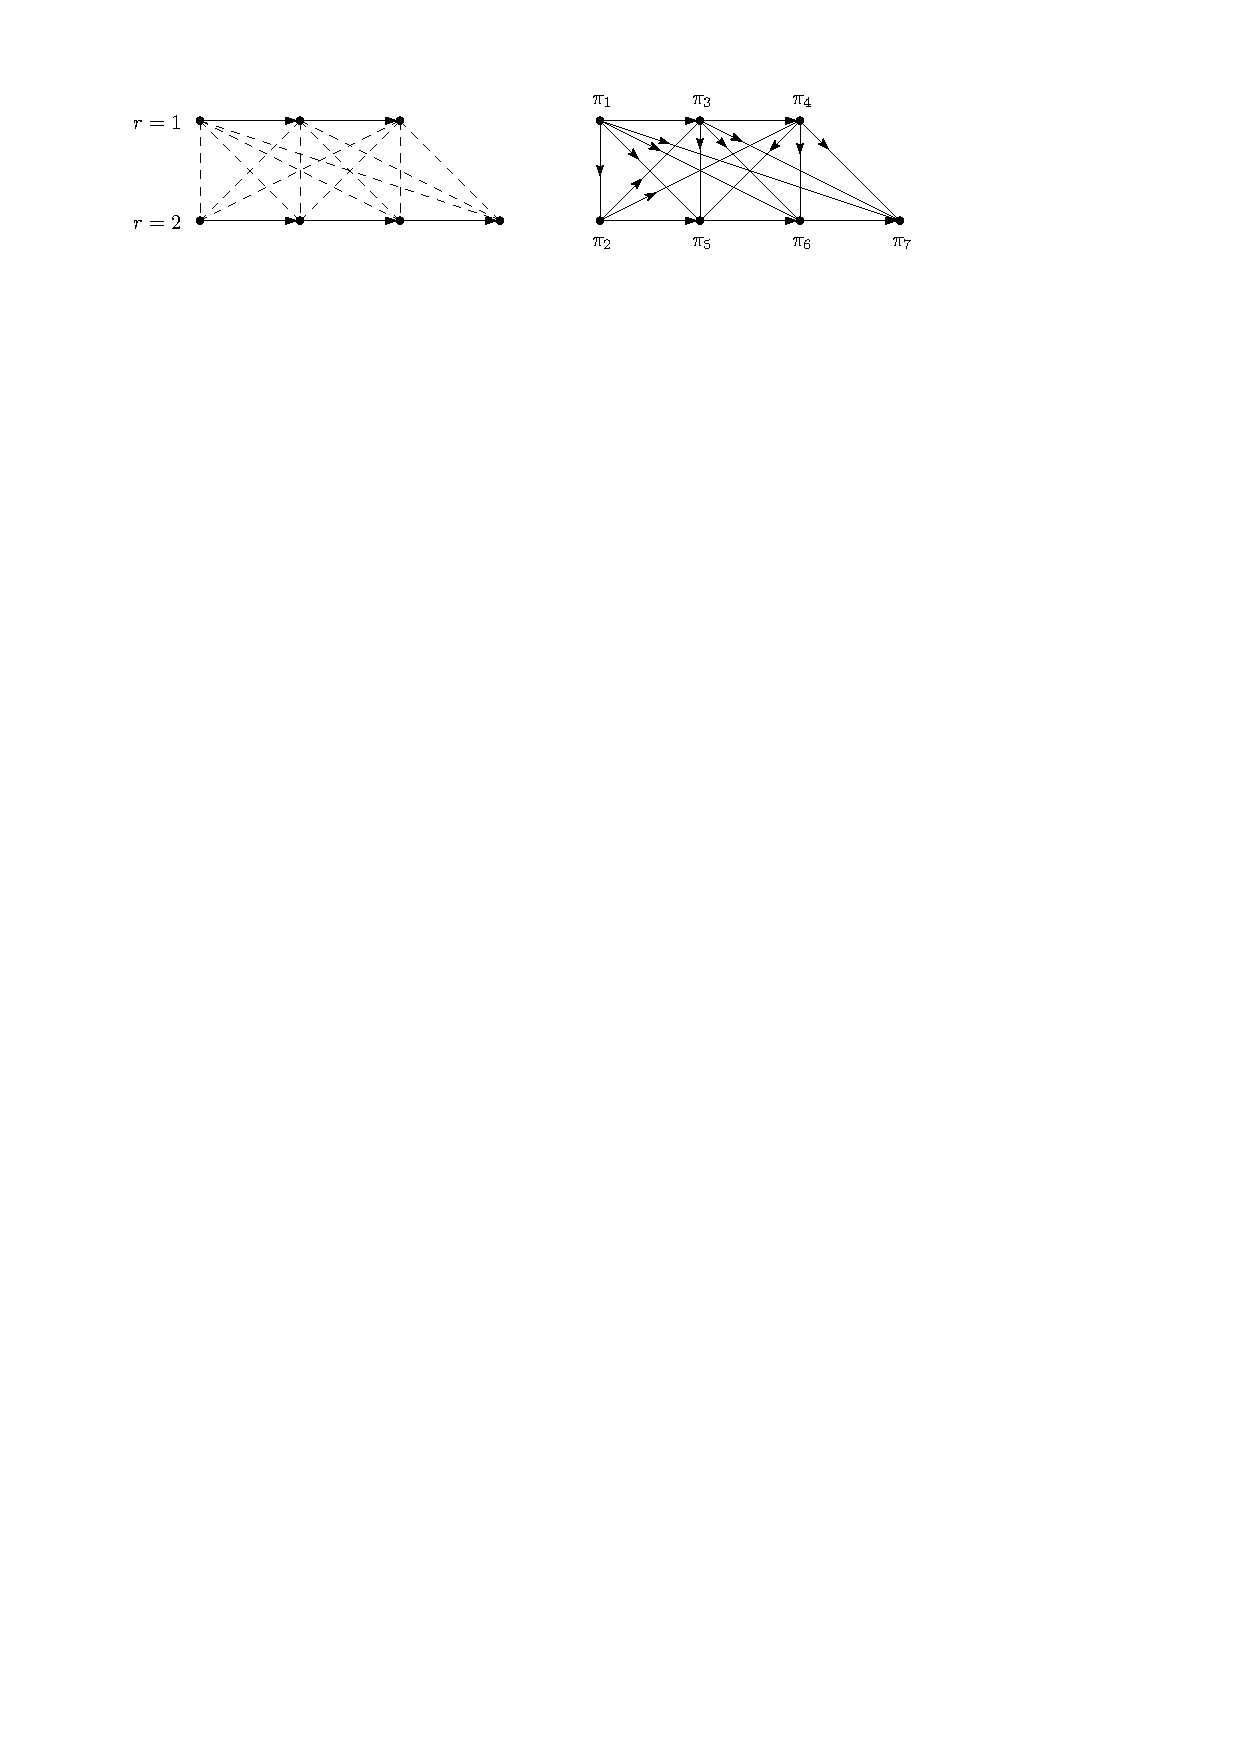
\includegraphics[width=0.98\textwidth]{figures/single/disjunctive_graph.pdf}
  \caption{Illustration of disjunctive graphs for the same instance as in
    Figure~\ref{fig:disjunctive-graph-intro}, again without dummy nodes. Horizontal arrows are the conjunctive
    arcs, the rest are disjunctive arcs. The left graph illustrates the \textit{empty}
    disjunctive graph; the dashed lines indicate an empty selection
    $\mathcal{O} = \varnothing$. The selection shown in the \emph{acyclic} and \emph{complete} graph on the
    right corresponds uniquely to the vehicle order
    $\nu = ((1,1), (2,1), (1,2), (1,3), (2,2), (2,3), (2,4))$ and the route order
    $\eta = (1, 2, 1, 1, 2, 2, 2)$.}\label{fig:disjunctive-graphs}
\end{figure}

\begin{theorem}
  Problem~\eqref{eq:C} is equivalent to the \emph{route ordering problem}
  \begin{align}
    \label{eq:RO}
    \min_{\eta \in E} \; \sum_{i \in \mathcal{N}} y_i(\eta) .
  \end{align}
\end{theorem}
\begin{proof}
  Let $\Omega$ denote thet set of all acyclic complete selections $\mathcal{O}$,
  and let $\mathcal{V}$ denote the set of vehicle orders, then we will show that there is
  a bijection between $\Omega$ and $\mathcal{V}$.
  %
  We already argued that there is a bijection between $\mathcal{V}$ and $E$, so from
  there, the desired result follows from
  Lemma~\ref{lemma:disj-graph-optimization}.

  Assume that $\mathcal{G}(\mathcal{O})$ is an acyclic complete disjunctive graph, then
  subgraph induced by the non-dummy nodes $\mathcal{N}$ is a DAG, so there must
  be some topological order $\nu$ of $\mathcal{N}$ by
  Lemma~\ref{lemma:minimal-node}.
  %
  It is clear that $\nu$ must respect the ordering of vehicles on routes, due to
  the conjunctive arcs, so it is clearly a vehicle order.
  %
  To show that $\nu$ is unique, suppose there is another topological order
  $\nu' \neq \nu$, then there must be at least one pair of indices
  $i,j \in \mathcal{N}$ that appears in opposite orders in $\nu$ and $\nu'$,
  say, $i$ appears before $j$ in $\nu$ and $j$ appears before $i$ in $\nu'$. It
  follows that $i$ and $j$ cannot both belong to the same route, because
  otherwise one of the topological orders would be invalid.
  %
  Therefore, $r(i) \neq r(j)$, but then we have either $(i,j) \in \mathcal{O}$
  or $(j,i) \in \mathcal{O}$, which shows again that one of $\nu$ or $\nu'$ must
  be invalid.
  %
  Hence, this $\nu(\mathcal{O}) = \nu$ is the unique vehicle order belonging to
  selection $\mathcal{O}$.

  Suppose we are given some vehicle order $\nu$, then it is straightforward to
  construct the corresponding disjunctive graph as follows.
  %
  Starting with an empty selection, we visit the non-dummy nodes in order $\nu$
  and for each node $\nu_k$, we just add all disjunctive arcs
  $\nu_k \rightarrow v$ such that $r(v) \neq r(\nu_k)$ and $v \in \mathcal{N}$
  has not yet been visited before.
  %
  This way, we end up with a unique acyclic complete selection
  $\mathcal{O}(\nu)$.
\end{proof}

\paragraph{Delay objective.}
We make one more slight change to the problem. Until now, we have been using the
total sum of crossing times as our objective. This captures our goal of
minimizing the travel delay of vehicles and has been convenient in terms of
notation. However, from now on, we will consider the total delay, which is the
sum of $y_i - a_i$ over all vehicles $i$.
%
In the remainder of this chapter, we focus on solving the following equivalent
problem.

\begin{define}
  The route ordering problem with delay objective is defined as
  \begin{align}
    \label{eq:D}\tag{D}
    \min_{\eta \in E} \; \sum_{i \in \mathcal{N}} y_i(\eta) - a_i .
  \end{align}
  %
  An instance of this problem is uniquely identified by the tuple
  $(\mathcal{N}, a, \rho, \sigma)$.
\end{define}


\clearpage

\section{Scheduling as learning problem}\label{sec:seq-modeling}

We will now explain how the general ML for CO framework presented in Section~\ref{sec:ml-co}
can be applied to the route ordering problem~\eqref{eq:D}.
%
As we discussed before, the most important decision is the design of the state
space of the MDP algorithm model, since this essentially determines the class of
algorithms over which we are optimizing---it is our main way of incorporating
prior knowledge and intuition into the model.
%
We will now show how the findings of the previous section leads to a natural
choice of states and corresponding algorithmic structure.

\paragraph{Constructive scheduling.}
In the previous section, we have shown that the crossing time scheduling
problem~\eqref{eq:C}, stated in terms of finding crossing times $y_i$, is equivalent to
the problem~\eqref{eq:D}, stated in terms of finding an optimal route order $\eta \in E$.
Given such a route order $\eta$, we can obtain the corresponding crossing time
schedule $y(\eta)$ by solving the linear program~\eqref{eq:active_schedule} or by using the simple
procedure described in the proof of Lemma~\ref{lemma:unique-active-schedule}.
%
Instead of searching directly over all feasible $\eta \in E$, we propose to search
for a good \emph{constructive policy}, which is essentially a procedure to build the
optimal schedule in a step-by-step fashion. This approach is particularly suited
to capture within the MDP framework.

% informal description
The basic idea is as follows.
%
Each state encodes a partial schedule, in which only the first few vehicles on
each route---according to their relative order---are said to be
\emph{scheduled}.
%
Initially, all vehicles are unscheduled.
%
Each step in the MDP corresponds to picking some route and then adding the next
unscheduled vehicle on that route to the schedule.
%
This way, we obtain a sequence of \emph{partial schedules}, encoded as
disjunctive graphs, until we arrive at a complete schedule.


\subsection{Constructive scheduling MDP}\label{sec:MDP}

% \begin{itemize}
%   \item input = instance $s = (\mathcal{N}, a,\rho, \sigma)$
%   \item initial state = $\mathcal{G}_0$ belonging to instance $s$
%   \item states are disjunctive graphs $\mathcal{G}_t$
%   \item actions are routes $\mathcal{R}$
%   \item transitions: add arcs to disjunctive graph
%   \item output = schedule $y = y(\mathcal{G}_N) = y(\mathcal{O}_N) = y(\eta)$ as a function of final disjunctive graph
%   \item final reward $m(s, \pi) = \sum_i y_i$
%   \item The total number of vehicles $N$ in the system is the fixed episode length.
% \end{itemize}

% instance -> empty disjunctive graph
We start by defining the \emph{single-instance} MDP, denoted $\mathcal{M}^s$,
given some problem instance specification $s = (\mathcal{N}, a, \rho, \sigma)$
for the route ordering problem~\eqref{eq:D}.

\paragraph{States and decision epochs.}
The initial state is the unique empty disjunctive graph $\mathcal{G}_0^s$
corresponding to instance $s$. To keep notation light, we will drop the
superscript $s$. All vehicles are said to be \emph{unscheduled} in $\mathcal{G}_0$.
%
In each step, we add some vehicle to the partial schedule, until all vehicles
are scheduled.
% decision epochs
Therefore, the MDP has exactly $N$ decision epochs\footnote{This corresponds to
  a \emph{finite-horizon} of size $N+1$ in the usual formal MDP definition, see
  Appendix.}, where $N$ is the total number of vehicles.
%
Each intermediate state $\mathcal{G}_t$ is some partial disjunctive graph,
encoding the current partial schedule.
%
Next, we define the actions and transitions such that the final state
$\mathcal{G}_N$ is guaranteed to represent a complete schedule.

\paragraph{Actions and transitions.}

Vehicles are added to the partial schedule according to the relative order in
which they appear on their route. To make this precise, let $k_r(\mathcal{G}_t)$
denote the number of vehicles on route $r$ that are \emph{scheduled} in state
$\mathcal{G}_t$.
%
Initially we have $k_r(\mathcal{G}_0) = 0$ for all $r \in \mathcal{R}$.
%
At every decision epoch, we choose some route $r$ that has some unscheduled
vehicles left. Hence, the set of admissible actions at state $\mathcal{G}_t$ is
defined as
\begin{align}
  \label{eq:5}
  \mathcal{A}(\mathcal{G}_t) := \{ r: k_r(\mathcal{G}_t) < n_r \} .
\end{align}
%
Suppose we take action $r$, then the first unscheduled vehicle on route $r$ is
\begin{align}
  i = (r, k_r(\mathcal{G}_t) + 1).
\end{align}
%
We include vehicle $i$ in the partial schedule by adding the disjunctive arcs
\begin{align}
  \label{eq:disj-arcs}
  \big\{ i \rightarrow (r', k) : r' \neq r, \;  k \in \{ k_{r'}(\mathcal{G}_t) + 1, \dots, n_{r'} \} \big\}
\end{align}
to $\mathcal{G}_t$ to obtain the next state $\mathcal{G}_{t+1}$.
%
Note that~\eqref{eq:disj-arcs} are all the disjunctive arcs from $i$ to each
unscheduled vehicle on all other routes.
%
With these deterministic transitions, it is easy to verify that each partial
disjunctive graph $\mathcal{G}_t$ encodes a partial vehicle and route order
\begin{align}
  \nu_{1:t} = (\nu_1, \dots, \nu_t) \quad \text{ and } \quad \eta_{1:t} = (\eta_1,\dots, \eta_t) ,
\end{align}
in the sense that $\nu_{1:t}$ is the unique topological order of the vehicles in
$\mathcal{G}_t$ that are scheduled.
%
In other words, each transition appends an unscheduled vehicle at the end of the
current vehicle order encoded by $\mathcal{G}_t$.
%
Furthermore, since $\eta_t$ is the route that was chosen as action to arrive at
the next partial schedule, we could write each particular transition as
$\mathcal{G}_{t-1} \xrightarrow{\eta_{t}} \mathcal{G}_{t}$.

\paragraph{Final state.}
After $N$ steps, all vehicles are scheduled and the final state $\mathcal{G}_N$
must be a complete acyclic disjunctive graph, because we never introduce arcs to
nodes that already have outgoing disjunctive arcs. Therefore, $\mathcal{G}_N$
corresponds to a valid route order $\eta_{1:N} \in E$, thereby encoding an
active schedule $y(\eta_{1:N})$. \comment{Introduce additional notation, if
  neccessary. For example, introduce $\eta(\mathcal{G})$ (or with sequence
  notation $\eta_{1:t} = \eta(\mathcal{G}_t)$) as the partial route sequence
  belonging to the partial disjunctive graph. This can be interpreted as a sort
  of \emph{read-out} function to obtain the solution from the final state. Prove
  that the complete disjunctive graph $\mathcal{G}_N$ is always acyclic and
  complete, such that $y(\eta(\mathcal{G}_N))$ is a valid active schedule. [
  optional: example MDP with example transitions ]}
%
This means that the quantity
\begin{align}
  \sum_{i \in \mathcal{N}} a_i - y_i(\eta_{1:N})
\end{align}
is a natural candidate to use as the definition of the final reward. Note that
the sign is reversed with respect to the original objective in~\eqref{eq:D},
because the convention is that we aim to maximize reward.
%
However, a single final reward is not convenient in practice. It is often better
for convergence of the learning algorithm when rewards happen more evenly
throughout the episode.
%
Therefore, we will show next how such a \emph{dense reward} can be defined based
changes of certain lower bounds.

\paragraph{Dense rewards.}

First, we show that the active schedule belonging to each partial disjunctive
graph provides a lower bound on the crossing times of the final schedule.
%
% crossing time lower bounds
Each disjunctive graph $\mathcal{G}_t$ encodes a selection $\mathcal{O}_t$ of
disjunctive arcs.
%
Suppose that the selection is not yet complete and let $y(\mathcal{O}_t)$ be the
corresponding active schedule.
%
Observe that adding more disjunctive arcs to $\mathcal{G}_t$ can only cause the
crossing times of the corresponding active schedule to increase with respect to
$y(\mathcal{O}_t)$, because additional constraints are added to the linear
program~\eqref{eq:active_schedule}.
%
This proves the following result.
%
\begin{lemma}
  Let $\mathcal{O} \subseteq \mathcal{O}^*$ be two acyclic selections of disjunctive
  arcs and let $y = y(\mathcal{O})$ and $y^* = y(\mathcal{O}^{*})$ denote the
  corresponding active schedules, then $y^{*}_i \geq y_i$ for all
  $i \in \mathcal{N}$.
\end{lemma}
\noindent
Given some disjunctive graph $\mathcal{G}_t$ with selection $\mathcal{O}_t$, we
define the \emph{crossing time lower bounds}
\begin{align}
  \beta_t(i) = y_i(\mathcal{O}_t) \quad \text{ for each } i \in \mathcal{N} .
\end{align}
%
These values can be interpreted as providing lower bounds on the crossing times
for any \emph{completion} of the current disjunctive graph and satisfy the
following three properties:

\begin{enumerate}[label=(\roman*)\;\;,leftmargin=3.5em,midpenalty=5]
  \item Recall that the earliest crossing times $a$ need to satisfy
        $a_i + \rho \leq a_j$, see Lemma~\ref{lemma:arrivals}. Since the empty
        disjunctive graph consists of only a single chain of conjunctive arcs
        per route, this implies that the initial lower bounds are given by
        \begin{align}
          \beta_0(i) = a_i \quad \text{ for all } i \in \mathcal{N}.
        \end{align}

  \item Each final state $\mathcal{G}_N$ corresponds to a complete selection
        $\mathcal{O}_N$. Hence, the final crossing time lower bounds
        are precisely the crossing times of the active schedule encoded by the
        complete disjunctive graph:
        \begin{align}
          \beta_N(i) = y_i(\eta_{1:N}) = y_i(\mathcal{O}_N) \quad \text{ for all } i \in \mathcal{N}.
        \end{align}

  \item Let $i$ be some vehicle that is scheduled at step $t$, then observe that
        future steps of the MDP will not introduce any more disjunctive arcs to
        $i$, which means that it is already the final crossing time:
        \begin{align}
          \beta_t(i) = \beta_{t+1}(i) = \dots = \beta_N(i) .
        \end{align}

\end{enumerate}

The dense rewards are now defined as follows. For each transition
$\mathcal{G}_{t-1} \xrightarrow{\eta_{t}} \mathcal{G}_{t}$, we define the
corresponding reward to be
\begin{align}
  r_t = r(\mathcal{G}_{t-1}, \eta_t, \mathcal{G}_t) = \sum_{i \in \mathcal{N}} \beta_{t-1}(i) - \beta_{t}(i) .
\end{align}
Hence, when the episode is done after $N$ steps, the total episodic
reward is given by the telescoping sum
\begin{align}
  \sum_{t=1}^{N} r_{t} = \sum_{i \in \mathcal{N}} \beta_{0}(i) - \beta_{N}(i)  = \sum_{i \in \mathcal{N}} a_{i} - y_{i}(\eta_{1:N}) ,
\end{align}
so maximizing the episodic reward corresponds to minimizing the delay objective
of~\eqref{eq:D}.

\begin{remark}
  Let us make a brief remark on implementing the above MDP in a computer
  program.
  %
  Instead of recomputing all the crossing time lower bounds $\beta$ at each step
  of the MDP, we can do a partial update as follows, which makes the
  implementation more efficient.
  %
  Let $\mathcal{G}_t$ be the current state and let $\eta_t$ denote the next
  action, which means that vehicle $i = (\eta_t, k_t(\eta_t))$ will be added to
  the schedule.
  %
  We just copy all the lower bounds by setting $\beta_{t+1} = \beta_t$ and then
  make the necessary updates as follows.
  %
  For each other route $r \neq \eta_t$, observe that $j = (r, k_t(r))$ is the
  first unscheduled vehicle. Because the disjunctive arc $i \rightarrow j$ gets
  introduced, we need to update
  \begin{align*}
    \beta_{t+1}(j) = \max(\beta_t(j), \; \beta_t(i) + \sigma ) .
  \end{align*}
  %
  When $\beta_{t+1}(j) = \beta_t(j)$, we say this update was void. If the update
  was not void, we only have to propagate this change along the chain of
  conjunctive arcs starting from $j$, because these unscheduled vehicles do not
  have any outgoing disjunctive arcs. Let such conjunctive chain be denoted by
  $j = (r,k) \rightarrow (r,k+1) \rightarrow \dots \rightarrow (r,n_r)$, then we
  update
  \begin{align*}
    \beta_{t+1}(r,l + 1) = \max(\beta_t(r,l + 1) , \; \beta_t(r,l) + \rho) ,
  \end{align*}
  in a loop where $l$ steps from $k$ to $n_r - 1$. Once such update is void, we
  know that all remaining updates will also be void, so we can simply stop the
  loop.
\end{remark}

\subsection{Generalization and learning objective}

We will now zoom in a little bit on how the MDP introduced above depends on a
particular instance specification $s = (\mathcal{N}, a, \rho, \sigma)$. Let
$\mathcal{R} = \{1, \dots, R\}$ denote the set of routes implicitly defined by
$\mathcal{N}$.
%
The MDP is defined in the previous section can be concisely written as
\begin{align}
  \mathcal{M}^s := (\mathcal{S}^s, \mathcal{A}^s, p^s, r^s) ,
\end{align}
where $\mathcal{S}^s$ is the state space, which is finite set of all possible
disjunctive graphs that can be encountered during the constructive scheduling
procedure, $\mathcal{A}^s$

It is not difficult to see that this set can be further written as the following
disjoint union of sets
\begin{align}
  \label{eq:8}
  \mathcal{S}^s = \mathcal{S}_1^s \sqcup \mathcal{S}_2^s \sqcup \dots \sqcup \mathcal{S}_N^s ,
\end{align}
where each $\mathcal{S}_t^s$ denotes the disjunctive graph obtained from
$\mathcal{G}_0^s$ after adding exactly $t$ vehicles.

Some brief discussion of what the learning objective is are in order here.

\note{[construct the joint MDP]}

\clearpage

\subsection{Optimal policies and parameterizations}

\comment{Why parameterize at all? Because it is not guaranteed that the policy space is finite.}

Narrow the space of policies to optimize over without losing optimality guarantees.
%
After that, we propose a very simple and natural parameterization of policies
that is inspired by the platoon preservation theorem. This parameterization is
however not very suited to gradient-based optimization. Therefore, we propose a
generalization of this parameterization that can be readily approached using
standard policy gradient-based optimization, which is discussed in the next
section.

\paragraph{MDP and policy classes.}

Define general infinite-horizon MDP.
Define policies as sequence of decision rules.
Explain non-stationary vs. stationary policies.
Let $\bar{\Pi}$ denote the set of all policies.
Let $\Pi$ denote the set of all stationary policies.
Mention Markovian and history-dependent policies, but refer to Puterman for details.
Let $\Pi_\text{det}$ denote the set of all deterministic stationary policies.


\begin{theorem}
  There exists an optimal policy $\pi^* \in \bar{\Pi}$ for our scheduling MDP
  that is stationary and deterministic, so $\pi^* \in \Pi_\text{det}$.
\end{theorem}
\begin{proof}
  Stationarity is the most important to show.
\end{proof}

\note{Show that our deterministic MDP has an optimal policy that is stationary
  and deterministic.} \note{From now on we only consider $\Pi_\text{det}$}.

\paragraph{Deterministic MDP with deterministic policies.}

Let $\mathcal{S}$ be the set of states. Let $\mathcal{A}(s) \neq \varnothing$ be
the set of admissible actions when in state $s \in \mathcal{S}$. Let
$p : \mathcal{S} \times \mathcal{A} \rightarrow \mathcal{S}$ be the transition
function and $r : \mathcal{S} \times \mathcal{A} \rightarrow \mathbb{R}$ the
reward function.
We emphasize that $p$ may encode so-called \emph{self-loops}, so it perfectly
fine to set $p(s, a) = s$ for all $a \in \mathcal{A}(s)$, such a state $s$ is
called a \emph{terminal state}. This allows us to model processes of finite
length within this general infinite-horizon framework.

Let $\Pi_\text{det}$ denote the set of admissible deterministic stationary
policies, which are all functions $\pi: \mathcal{S} \rightarrow \mathcal{A}$
that satisfy $\pi(s) \in \mathcal{A}(s)$ for all $s \in \mathcal{S}$.
%
Given some policy $\pi \in \Pi_\text{det}$ and state $s_0 \in \mathcal{S}$, let
the \emph{rolled-out} episode $\tau$ be defined as the infinite sequence
\begin{align}
  \tau = (s_0, a_1, r_1, s_1, a_2, r_2, s_2, \dots) ,
\end{align}
such that $s_{t+1} = p(s_t, a_{t+1})$ and $r_{t+1} = r(s_t, a_{t+1})$ for all
$t \in \{ 0, 1, 2, \dots \}$.

\paragraph{State abstraction.}

Let $\phi : \mathcal{S} \rightarrow \bar{\mathcal{S}}$ be some function that
takes each state $s$ from the so-called \emph{ground MDP} to a so-called
\emph{abstract state} $\bar{s}$.
%
The idea is that some parts of the state may be irrelevant for the agent to make
optimal decisions, see also Figure~\ref{fig:state-abstraction}.
%
% Every state abstraction naturally induces equivalence classes on the state
% space: every $s_1, s_2 \in \mathcal{S}$ such that $\phi(s_1) = \phi(s_2)$
% belong to the same equivalence class.
%
We say that some deterministic policy $\pi \in \Pi_\text{det}$ is an
\emph{abstract} policy with respect to $\phi$ when we have $\pi(s_1) = \pi(s_2)$
for all $s_1, s_2 \in \mathcal{S}$ such that $\phi(s_1) = \phi(s_2)$.
%
Let the class of all deterministic abstract policies with respect to $\phi$ be
denoted by $\Pi_\phi$.

\begin{figure}[h]
\centering
\tikzstyle{block} = [rectangle, draw,
    text width=7em, text centered, rounded corners, minimum height=4em]
\tikzstyle{phi} = [draw, fill=white, minimum size=12pt, inner sep=1pt, font=\small]
\tikzstyle{line} = [draw, -latex]
\begin{tikzpicture}[node distance = 6.5em, auto, thick]
  \node [block] (Agent) {Agent};
  \node [block, below of=Agent] (Environment) {Environment};

    \path [line] (Agent.0) --++ (4em,0em) |- node [near start]{Action $a_t$} (Environment.0);
    % \path [line] (Environment.190) --++ (-6em,0em) |- node [near start] {New state  $s_{t+1}$} (Agent.170);
    \path [line] (Environment.170) --++ (-4.25em,0em) |- node [near start, right] {Reward $r_{t+1}$} (Agent.190);

  \draw [line] (Environment.190) --++ (-6em,0em) |-
      node[left, align=center, yshift=-45pt]{Ground state $s_{t+1}$}
      node[midway, phi, yshift=-35pt] {$\phi$}
      node[left, align=center, yshift=-10pt]{Abstract state $\bar{s}_{t+1}$}
      (Agent.170);
\end{tikzpicture}
\caption{Reinforcement learning control loop with state abstraction $\phi$
  placed between the state signal and the agent.}\label{fig:state-abstraction}
\end{figure}


\paragraph{State abstraction.}

Once vehicle $i$ has been scheduled in step $t$, it can be shown that the policy
does not need to take into account any information related to this vehicle
anymore in order to complete the schedule.
%
For example, in the remaining steps, the policy should no longer depend on
$\beta_t(i)$.
%
Generally speaking, there exists some \emph{observation mapping} $\phi : \mathcal{S} \rightarrow \mathcal{X}$, mapping states to the \emph{observation space} $\mathcal{X}$, such that the class
\begin{align}
  \Pi_\phi := \{ \pi : \pi = f(\phi(s)) , \text{ for some function } f : \mathcal{X} \rightarrow \Delta(\mathcal{A}) \}
\end{align}
contains some policy $\pi^* \in \Pi_\phi$ that is optimal with respect to all policies.
%
The general notion of ignoring irrelevant state information is known as
\emph{state abstraction}. \note{[cite]}

\paragraph{Horizon observation.}
This irrelevance leads us to define some sort of \emph{horizon} observation of crossing
time lower bounds and some auxiliary flags, involving only the unscheduled
vehicles.
%
Let $\bar{\beta}_t$ denote the minimum crossing time lower bound of all unscheduled
vehicles.
%
Consider some route $r \in \mathcal{R}$ and let $k = k_t(r)$ denote the number
of scheduled vehicles, such that $(r, k+1)$ is the first unscheduled vehicle on
this route, then the horizon $h_t(r)$ at this route is defined to be the
sequence
\begin{align}
  h_t(r) := (\beta_t(r, k + 1) - \bar{\beta}_t, \; \beta_t(r, k + 2) - \bar{\beta}_t, \; \dots , \; \beta_t(r, n_r) - \bar{\beta}_t) .
\end{align}
%
The total $\beta$-horizon is now given by the vector
$h_t = (h_t(1), \dots, h_t(R))$.

% Define pastel colors
\definecolor{pastelblue}{RGB}{179,205,227}
\definecolor{pastelorange}{RGB}{251,180,174}
\definecolor{pastelgreen}{RGB}{170, 210, 170}

% \begin{figure}[h]
% \centering
% \begin{tikzpicture}

% \pgfmathsetseed{1}

% \def\width{1.2}
% \def\height{0.5}

% \tikzset{
%     rect/.style={
%         % draw,
%         minimum width=\width,
%         minimum height=\height,
%         thick,
%         align=center
%     }
% }

% \def\routespace{1.2}

% \foreach \r/\color in {1/pastelblue,2/pastelorange,3/pastelgreen} {
%   \pgfmathsetmacro{\x}{0}
%   \foreach \k in {1,...,5} {
%     \node[rect, fill=\color] (\r-\k) at (\x, -\routespace * \r) {(\r,\k)};
%     \pgfmathparse{\x + \width + rnd*0.8}
%     \global\let\x\pgfmathresult
%   }
% }

% \begin{pgfonlayer}{background}
%   \node[fill=gray!15, rounded corners, fit=(1-1)(1-5), inner sep=0.2cm] {};
%   \node[fill=gray!15, rounded corners, fit=(2-1)(2-5), inner sep=0.2cm] {};
%   \node[fill=gray!15, rounded corners, fit=(3-1)(3-5), inner sep=0.2cm] {};
% \end{pgfonlayer}

% \end{tikzpicture}
% \end{figure}

% -----

\paragraph{Platoon preserving policies.}

Before we propose concrete parameterizations of $\pi$, we will first derive two
rules that optimal policies must satisfy, thereby essentially reducing the
policy space.
%
As part of the structural analysis of problem~\eqref{eq:C} at the end of the previous
chapter, we discussed the platoon preservation Theorem~\ref{thm:exhaustive}, which states that
\begin{quote}
  If $y$ is an optimal schedule for~\eqref{eq:C}, satisfying $y_{i} + \rho \geq a_{j}$ for some
  $(i,j) \in \mathcal{C}$, then vehicle $i$ is followed immediately by $j$, so
  $y_{i} + \rho = y_{j}$.
\end{quote}
%
Roughly speaking, this means that whenever it is possible to schedule a vehicle
immediately after its predecessor on the same route, then this must be done in
an optimal schedule.
%
Observe that this rule essentially reduces the search space of feasible
schedules---it lead to the definition of three types of cutting planes.
%
Similarly, this rule can be transferred to the MDP context to reduce the space
of feasible policies as follows. Let $\mathcal{G}_t$ denote the current partial
schedule and assume that it is not an initial state, so $t \geq 1$. Let the
vehicle that was scheduled in the previous step be denoted by $i = (r, k)$ and
suppose $j = (r, k+1)$ exists.
%
As we argued above, $\beta_t(i) = y_{i}$ is the crossing time of vehicle $i$,
regardless of the remaining actions taken in the MDP.
%
Therefore, if we have
\begin{align}\label{eq:rule-exhaustive}
  \beta_t(i) + \rho \geq a(j),
\end{align}
then the platoon preservation rule requires the next action to be $r$.
%
Whenever a policy $\pi$ satisfies this rule, we say that it is
\emph{exhaustive}, so the platoon preservation theorem implies that each optimal
policy $\pi$ must be exhaustive.

\paragraph{Active policies.}
Next, we present yet another simple rule that each optimal policy $\pi$ must
satisfy.\comment{Better to first prove this rule for schedules (in the static
  sense), and then show that this transfers to a rule that optimal policies must
  satisfy.}
%
Again, let $i = (r,k)$ denote the last scheduled vehicle and assume
$j = (r,k+1)$ exists, so it is the next unscheduled vehicle on this route.
Suppose that
\begin{align}\label{eq:rule-active}
  \beta_t(j) + \rho + \sigma \leq a(u) ,
\end{align}
for each first unscheduled vehicle $u = (r', k_t(r'))$ on every other route
$r' \neq r$, then the next action must be $r$.
%
Whenever a policy $\pi$ satisfies this rule, we call it \emph{active}.
%
It is straightforward to see that optimal $\pi$ must be active: by
contradiction, if $j$ is not scheduled immediately after $i$, then we can move
it immediately after $i$, which is possible without affecting the crossing times
of other vehicles, so that we obtain a strictly better schedule.

\paragraph{Threshold heuristic.}
When neither of the conditions~\eqref{eq:rule-exhaustive}
or~\eqref{eq:rule-active} holds, there is still a lot of freedom to define the
concrete policy.
%
We will now define a concrete parameterizations of $\pi$ that has a particularly
simple interpretation.
%
The idea is to only consider the crossing time lower bound of the next
unscheduled vehicle on the route chosen in the last step. The idea is that we
aim to continue on the same route as long as possible, to avoid introducing
unnecessary switch-over time $\sigma$.
%
Recall that a platoon was defined as a sequence of consecutive vehicles
$(r, l+1), (r, l+2), \dots, (r, l+n)$ from some route $r$ such that
\begin{align*}
  a(r,k) + \rho = a(r, k+1)  \quad \quad \text{ for all } l < k < l + n.
\end{align*}
%
Note that the platoon preservation theorem essentially says that platoons should
be treated as a whole unit: given some other vehicle on a different lane, the
platoon is either scheduled entirely before it or entirely after it. In other
words, the platoon is never \emph{split} in an optimal schedule.
% generalize to "almost platoons"
Based on this idea, we might think that the same holds true whenever a vehicle
can be scheduled \textit{sufficiently} soon after its predecessor.
%
In other words, we might relax the definition of a platoon to
\begin{align}
  a(r,k) + \rho + \tau \geq a(r, k + 1) \quad \text{ for all } l < k < l + n,
\end{align}
for some small \emph{threshold} parameter $\tau \geq 0$.
%
Although the platoon preservation rule does not necessarily transfer to these
relaxed platoons, we can use it as the basis for a simple heuristic.
%
Consider the following rule
\begin{align}
  \text{ if } \; \beta_t(j) + \rho + \tau \geq a(j) , \; \text{ then next action is } \eta_t ,
\end{align}
where $\eta_t$ denotes the last scheduled route. Observe that this rule is a
direct generalization of~\eqref{eq:rule-exhaustive}.
%
When the condition does not hold, we choose the next route that has unscheduled
vehicles instead. The threshold heuristic is illustrated in
Figure~\ref{fig:threshold_heuristic}. \note{First action is ``earliest'' route.
  Add algorithm to precisely define the heuristic.}

% \begin{figure}
%   \centering
%   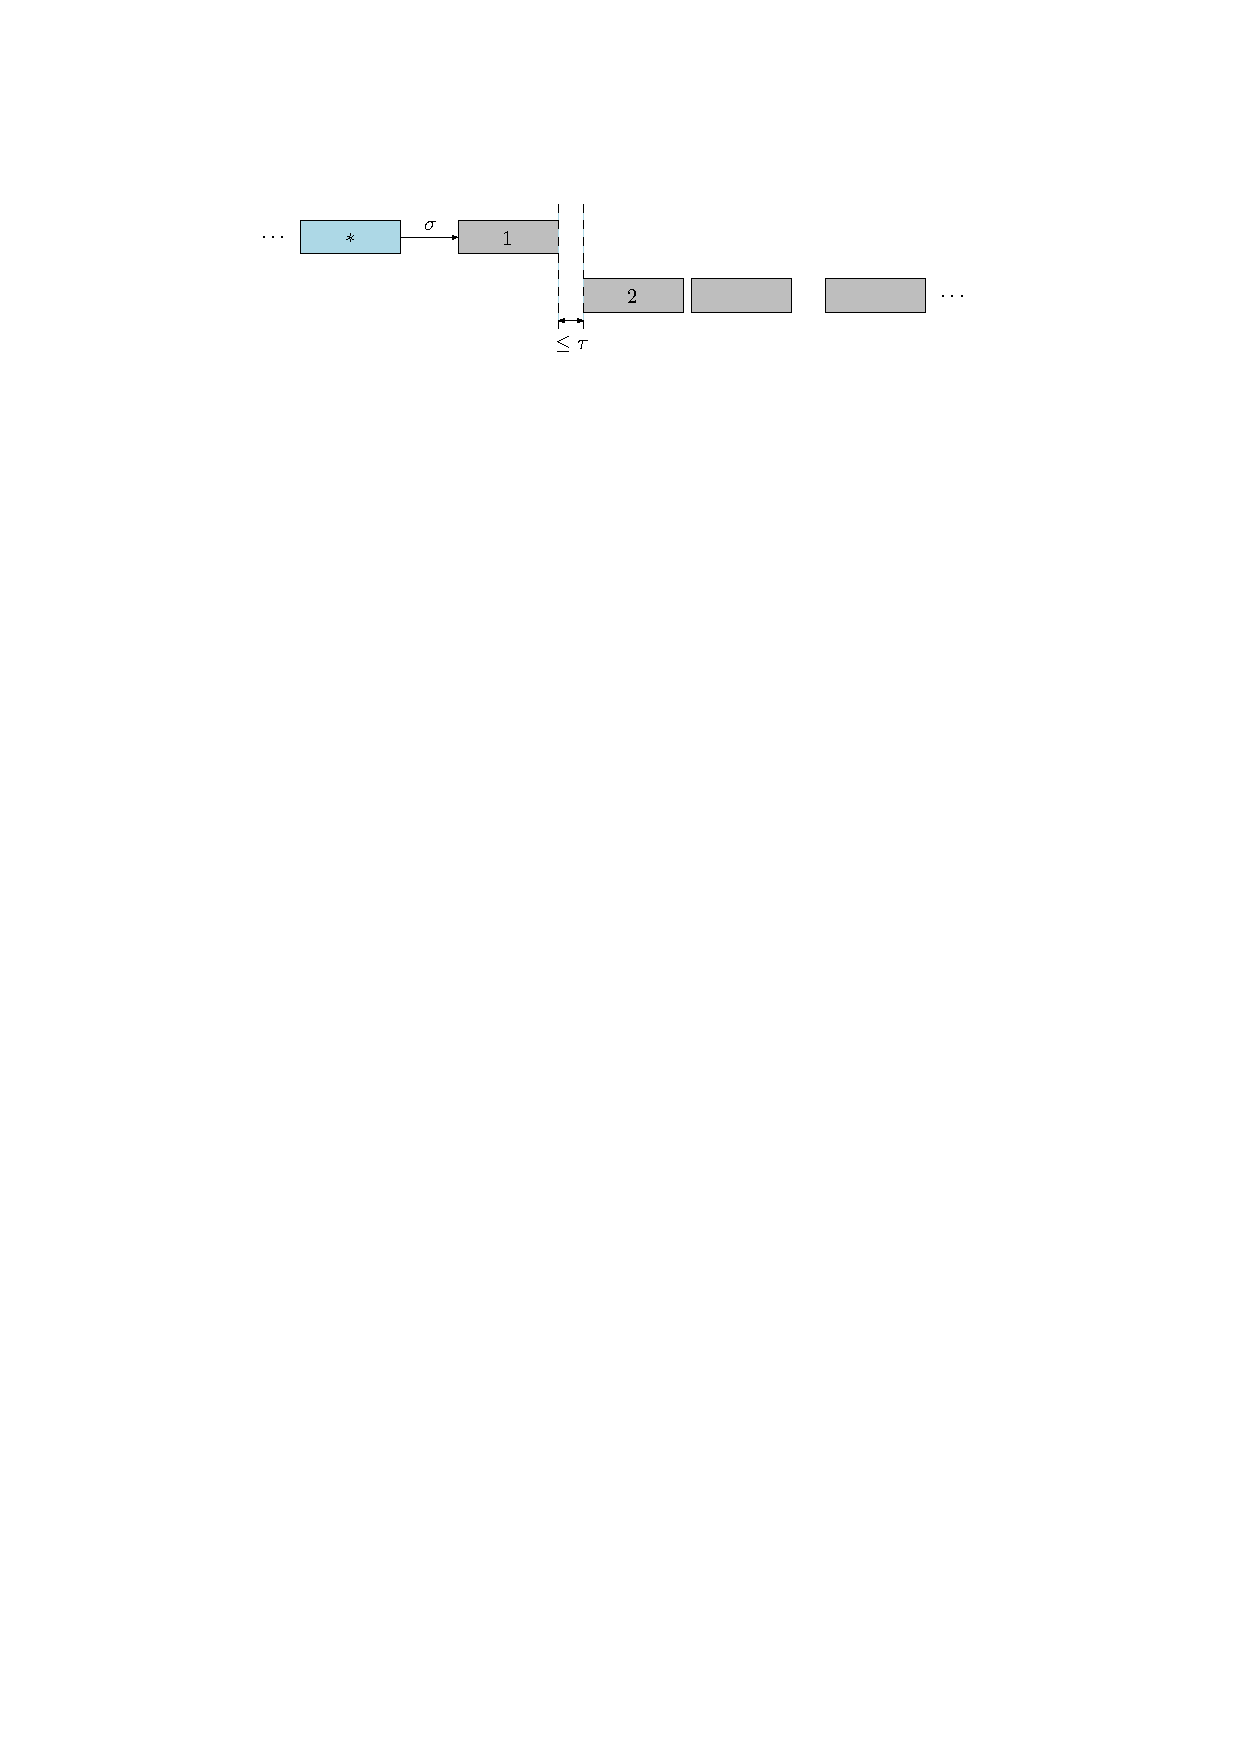
\includegraphics[width=0.8\textwidth]{figures/single/threshold}
%   \caption{Illustration of how the threshold heuristic is evaluated at some
%     intermediate step $t$ to choose the next route $\eta_{t+1}$. The top and bottom
%     row contains the unscheduled vehicles from route 1 and route 2,
%     respectively, drawn at their earliest crossing times $\beta_{t}(i)$. The middle
%     row represents the current partial schedule. Vehicle $\nu_{t-1}$ is from
%     route 1 and the last scheduled vehicle $\nu_{t}$ is from route 2 and the
%     disjunctive constraint for them happens to be tight in this case,
%     illustrated by the arrow. Whenever the indicated time difference is smaller
%     than $\tau$, the threshold rule selects vehicle $B$ to be scheduled next.
%     Otherwise, vehicle $A$ will be chosen.}\label{fig:threshold_heuristic}
% \end{figure}





\clearpage

\paragraph{Neural parameterization.}

We will now consider a parameterizaton that directly generalizes the
threshold heuristic. Instead of looking at the earliest crossing time of the
next vehicle in the current lane, we now consider the earliest crossing
times of all unscheduled vehicles across lanes.
%
The intuitive hypothesis is some sort of platoon preservation holds for
sequences of vehicles that are almost platoons.

\note{In the following definitions, we drop the step index $t$ to avoid
cluttering the notation.}

Next, we define some neural embedding $\bar{h}_{r}$ of each horizon. Observe
that horizons can be variable length. We could fix the length by using padding,
but this can be problematic for states that are almost done. Therefore, we
employ a recurrent neural network.

The main idea of recurrent neural networks is to share parameters $\theta$
across different sequence steps.
This way, we obtain a size-agnostic architecture.
%
Given input $x_n$ and internal \emph{state} $h_n$, produce output $o_n$ and next
state $h_{n+1}$, by some function
\begin{align}
  (o_{n}, h_{n+1}) = f_\theta(x_n, h_n) .
\end{align}

Each horizon $h_r$ is simply transformed into
a fixed-length embedding by feeding it in reverse order through a plain Elman
RNN. Generally speaking, the most recent inputs tend to have greater influence
on the output of an RNN, which is why we feed the horizon in reverse order, such
that those vehicles that are due first are processed last, since we expect those
should have the most influence on the decision.

These horizon embeddings are arranged into a vector $h_{t}$ by the following
cycling rule. At position $k$ of vector $h_{t}$, we put the embedding for route
\begin{align*}
  k - \eta_{t} \; \mathrm{mod} \; |\mathcal{R}|
\end{align*}
where $\eta_{t}$ denotes the last selected route. Using this cycling, we make sure
that the embedding of the last selected route is always kept at the same
position of the vector.
% \begin{align*}
%   {H}_{r} = \bar{h}(r - \eta_{t} \; \mathrm{mod} \; |\mathcal{R}|) ,
% \end{align*}
%
Using some fully connected neural network $f_{\theta}$ and a softmax layer, this
global embedding is then finally mapped to a probability distribution as
\begin{align*}
  \pi_{\theta}(\eta_{t+1} \, | \, \mathcal{G}_{t}) = \text{softmax} ( f_{\theta}(h_{t})) ,
\end{align*}
where $\theta$ denotes the parameters of $f$ and of the recurrent neural
networks.
% inference
After $\theta$ has been determined, we can apply greedy rollout by simply
ignoring routes that have no unscheduled vehicles left and take the argmax of
the remaining probabilities.

% \begin{figure}
%   \centering
%   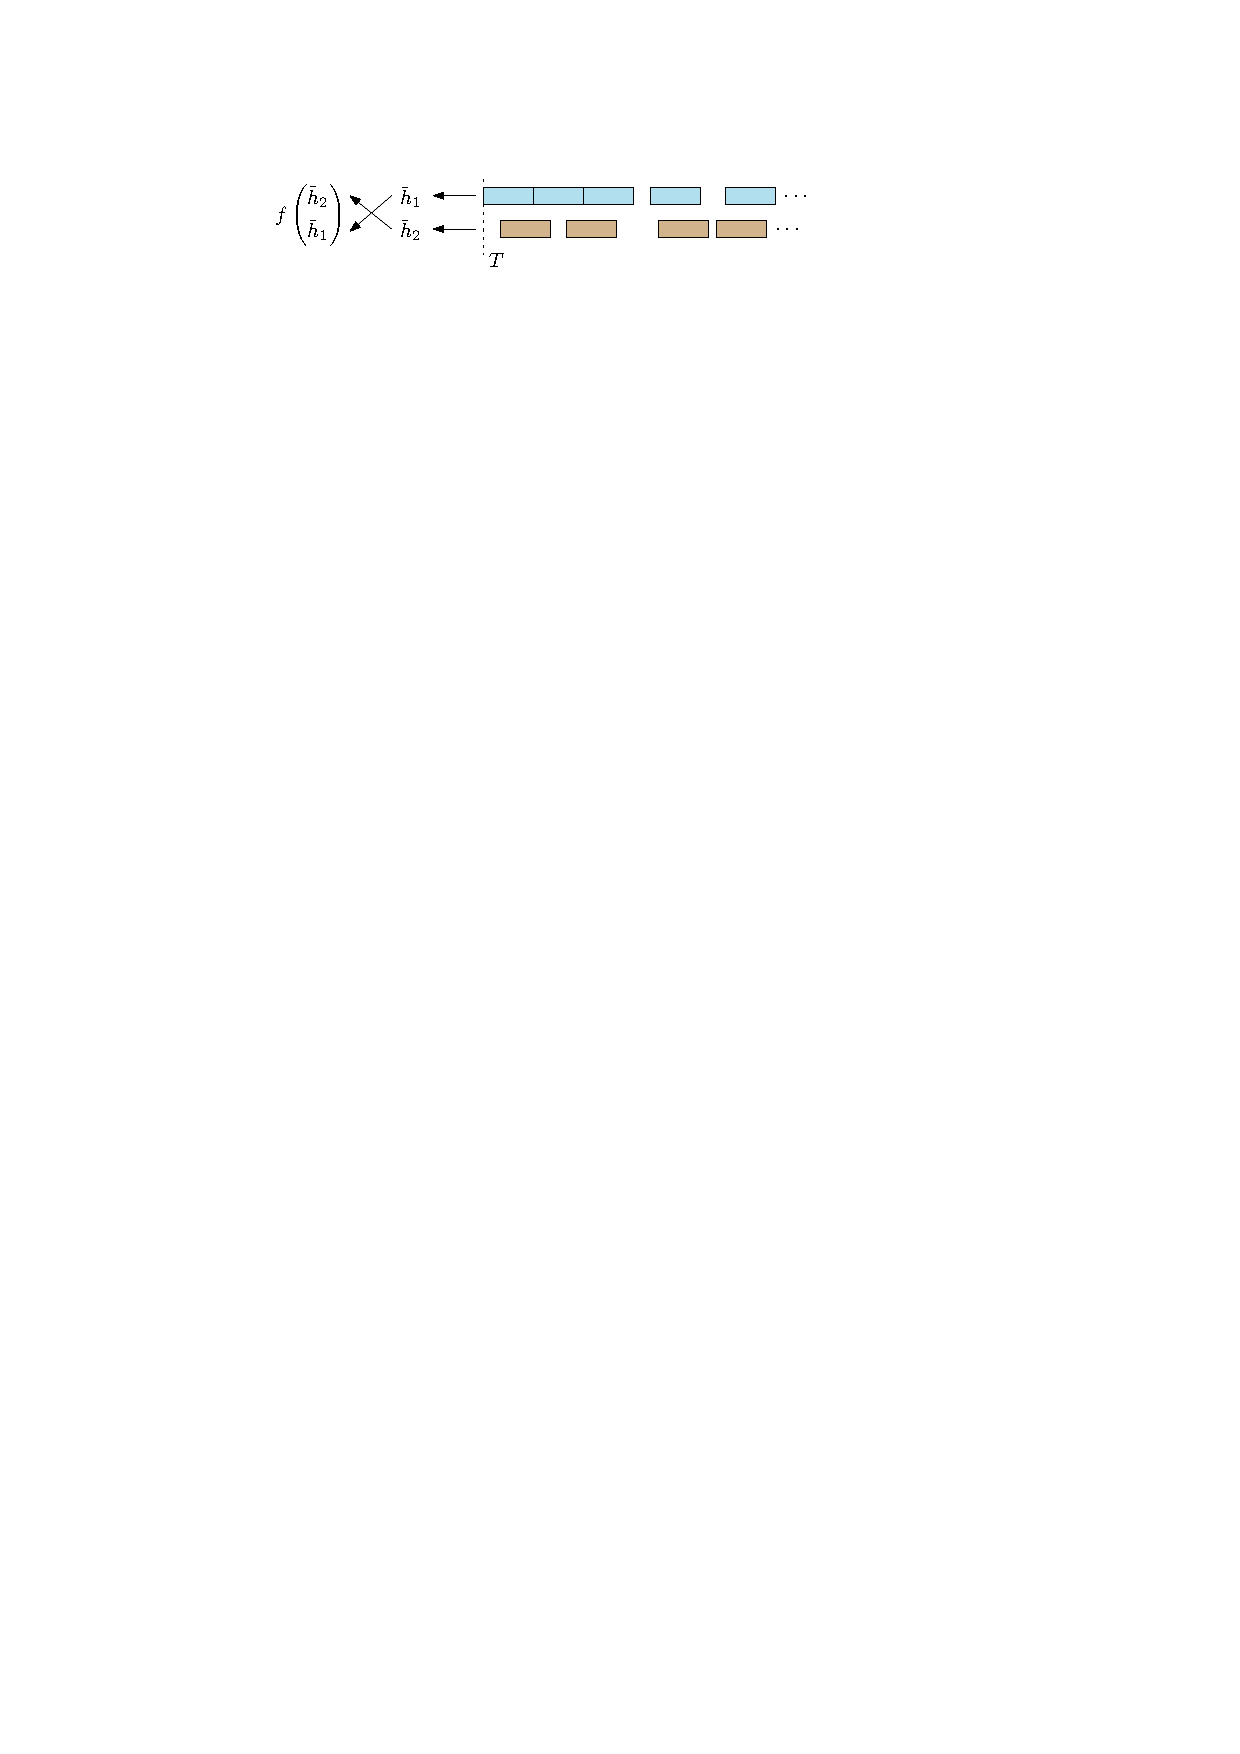
\includegraphics[width=0.8\textwidth]{figures/single/embedding}
%   \caption{Schematic overview of parameterization of the neural heuristic. The
%     distribution over the next route is parameterized as
%     $\pi_{\theta}(\eta_{t+1} | \mathcal{G}_{t})$, which is computed from the current route horizons
%     $h_{r}$ via embeddings $\bar{h}_{r}$ and the cyling trick. Observe that the
%     particular cycling shown in the figure corresponds to a situation in which
%     the current route is $\eta_{t} = 2$.}\label{fig:neural_embedding}
% \end{figure}



\clearpage

\subsection{Policy optimization}

Recall from Section~\ref{sec:ml-co} the abstract formulation of our goal to
develop an efficient algorithm for some combinatorial problem. Given some
distribution $P$ of relevant problem instances of
problem~\eqref{eq:C}, we aim to find a policy $\pi$ for
the MDP, defined in Section~\ref{sec:MDP}, that minimizes
\begin{align*}
  \min_{\pi \in \Pi} \mathbb{E}_{s \sim P} [m(s,\pi)] ,
\end{align*}
where $m(s, \pi)$ is some measure of performance of the policy, which can
include optimality of the produced solution or running time.
%
Since problem distribution $P$ is generally inaccessible and the space $\Pi$ of
valid policies is too large to consider entirely, we instead aim to minimize
\begin{align}
  \min_{\theta} \sum_{s \in D_\text{train}} \frac{1}{|D_\text{train}|} m(s, \pi_\theta) ,
\end{align}
where $D_\text{train}$ is some finite set of problem instances sampled from
distribution $P$.
%
The performance of an algorithm generally depends on the running time and the
quality of the solution obtained.
%
Furthermore, we also need to take into account the fact that optimizing $\theta$
takes time as well.
%
We will take the following approach.
%
Given some parameterization $\pi_\theta$ from above, this section will discuss how to optimize $\theta$ to obtain the best average performance on a set of training problem instances.
%
In the next section, we will evaluate the training time and evaluation time of
the trained policies.


\paragraph{Grid search for threshold heuristic.}
Given some instance $s$, let $\eta_{\tau}(s)$ be the schedule produced by the
threshold heuristic. Note that the objective is not differentiable with respect
to $\tau$, so we cannot directly use gradient-based optimization methods. However,
we only have a single parameter, so we can simply select the value of $\tau$ that
minimizes the average emperical objective
%
\begin{align}
  \min_{\tau \geq 0} \sum_{s \in D_\text{train}} \sum_{i \in \mathcal{N}} y_i(\eta_{\tau}(s)) ,
\end{align}
%
which can be approximated using a simple grid search.
%
We could also opt to approximate the class of threshold policies by using some
differentiable function to approximate the step function, but we will not
discuss this further.

\paragraph{Gradient-based imitation learning.}

Consider some instance $s \in D_\text{train}$ and let $\eta^{*}$ denote some optimal
route sequence, which can for example be computed by solving the MILP
formulation~\eqref{eq:C'}. For each such optimal schedule, we can compute the sequence
\begin{align*}
  \mathcal{G}_{0}, \eta_{1}, \mathcal{G}_{1}, \eta_{2}, \dots, \eta_{N}, \mathcal{G}_{N}.
\end{align*}
The resulting set of pairs $\{ (\mathcal{G}_{t}, \eta_{t+1}) : t = 1, \dots, N - 1 \}$
can be used to learn $\pi_{\theta}$ in a supervised fashion by treating it as a
classification task and computing the maximum likelihood estimator $\hat{\theta}$.
%
This approach of using so-called \textit{demonstration} to derive policies that are
similar to some \emph{expert policy} is generally refered to as
\textit{imitation learning}.
%
Let $Z$ denote the set of all state-action pairs collected from all
training instances $D_\text{train}$.
%
We make the procedure concrete for the case of two
routes $\mathcal{R} = \{ 1, 2 \}$, which is slightly simpler. Let $\pi_{\theta}(\mathcal{G}_{t})$
denote the probability of choosing the first route, then we can use the binary
cross entropy loss, given by
\begin{align}
  L_{\theta}(Z) := - \frac{1}{|Z|} \sum_{(\mathcal{G}, r) \in Z} \mathbf{1}\{r = 1\} \log(\pi_{\theta}(\mathcal{G})) + \mathbf{1}\{r = 2\} \log(1 - \pi_{\theta}(\mathcal{G})) ,
\end{align}
where $\mathbf{1}\{\cdot\}$ denotes the indicator function. Now we can simply rely on
some gradient-descent optimization procedure to minimize $L_{\theta}(Z)$ with
respect to $\theta$.

\paragraph{Policy gradient reinforcement learning.}

% imitation learning -> RL (on/off-policy)
Instead of using state-action pairs as examples to fit the model in a supervised
fashion (imitation learning), we can also choose to use the reinforcement
learning paradigm, in which the data collection process is guided by some
policy.


% REINFORCE
Policy-based methods work with an explicit parameterization of the policy. The
model parameters are then tuned based on experience, often using some form of
(stochastic) gradient descent to optimize the expected total return.
%
Therefore, the gradient of the expected return plays a central role. The
following identity is generally known as the Policy Gradient Theorem, where we
drop $\theta$ from $\pi_\theta$ to avoid cluttering the notation. The gradient
is with respect to the parameters $\theta$.
\begin{align*}
  \nabla \mathbb{E}_{\pi} G_{0} &\propto \sum_{s} \mu_{\pi}(s) \sum_{a} q_{\pi}(s, a) \nabla \pi(a | s, \theta) \\
  &= \mathbb{E}_{\pi}\left[ \sum_{a} q_{\pi} (S_{t}, a) \nabla \pi (a | S_{t}) \right] \\
  &= \mathbb{E}_{\pi}\left[ \sum_{a} \pi(a | S_{t}) q_{\pi} (S_{t}, a) \frac{\nabla \pi (a | S_{t})}{\pi (a | S_{t})} \right] \\
  &= \mathbb{E}_{\pi}\left[ q_{\pi} (S_{t}, A_{t}) \frac{\nabla \pi (A_{t} | S_{t})}{\pi (A_{t} | S_{t})} \right] \\
  &= \mathbb{E}_{\pi} \left[ G_{t} \log \nabla \pi (A_{t} | S_{t}) \right] .
\end{align*}
% \begin{align*}
%   \nabla \mathbb{E}_{a \sim p_{\theta}(a | s)} R(s, a) &= \nabla \sum_{a} p_{\theta}(a | s) R(s, a) \\
%   &= \sum_{a} \nabla p_{\theta}(a | s) R(s, a) \\
%   &= \sum_{a} p_{\theta}(a | s) \frac{\nabla p_{\theta}(a | s)}{p_{\theta}(a | s)} R(s, a) \\
%   &= \mathbb{E}_{a \sim p_{\theta}(a | s)} \left[  \frac{\nabla p_{\theta}(a | s)}{p_{\theta}(a | s)} R(s, a) \right] \\
%   &= \mathbb{E}_{a \sim p_{\theta}(a | s)} [ \nabla \log p_{\theta}(a | s) R(s, a) ] .
% \end{align*}
%
The well-known REINFORCE estimator is a direct application of the Policy
Gradient Theorem. At each step $t$, we update the parameters $\theta$ using a
gradient ascent update
\begin{align*}
  \theta \leftarrow \theta + \alpha G_{t} \nabla \log \pi_{\theta}(\eta_{t} | \mathcal{G}_{t}) ,
\end{align*}
with some fixed learning rate $\alpha$.
% add baseline to reduce variance
To reduce variance of the estimator, we can incorporate a so-called
\textit{baseline}, which is an estimate of the expected return of the current
state.
%
In the context of combinatorial optimization, the value of the baseline may be
interpreted as estimating the relative difficulty of an instance?

\paragraph{Beam search.}

Because the learned policy is still a stochastic policy, we need to specify how
to obtain a deterministic policy.
%
One way would be to calculate the maximum likelihood estimator
\begin{align*}
  \arg\max_{\eta} \pi_\theta(\eta | s) ,
\end{align*}
but this is generally very expensive to compute, because this could require
$O(R^{N})$ evaluations of $\pi_\theta(\eta_{t} | s, \eta_{1:t-1})$ when we do
not make additional structural model assumption.
%
Therefore, one often uses \textit{greedy rollout}, which means that we pick $\eta_{t}$ with
the highest probability at every step.
% other inference methods
Other inference strategies have been proposed in the context of modeling
combinatorial optimization problems, see for example the ``Sampling'' and
``Active Search'' strategies in the seminal
paper~\cite{belloNeuralCombinatorialOptimization2017}.


\clearpage
\section{Experimental results}\label{sec:results}

\note{indicate what low, med and high mean}

The evalutation of model performance is roughly based on two aspects. Of course,
the quality of the produced solutions is important. Second, we need to take into
account the time that the algorithm requires to compute the solutions. We need
to be careful here, because we have both training time as well as inference
time for sequence models.

Consider generalization along the two axes introduced in methodological
introduction of Section~\ref{sec:ml-co}.
%

% define \mathcal{N} through $vehicles per route
\paragraph{Instance specification.}

\note{Need to satisfy assumption on arrivals in definition of (D)}

% define a through a_r
For each route $r \in \mathcal{R}$, we model the sequence of earliest crossing times
$a_{r} = (a_{r1}, a_{r2}, \dots)$ as a stochastic process, to which we refer as
the \textit{arrival process}. Recall that constraints~\eqref{eq:conjunctive}
ensure a safe following distance between successive vehicles on the same route.
Therefore, we want the process to satisfy
\begin{align*}
  a_{(r, k)} + \rho_{(r,k)} \leq a_{(r, k + 1)} ,
\end{align*}
for all $k = 1, 2, \dots$.
%
Let the interarrival times be denoted as $X_{n}$ with cumulative distribution
function $F$ and mean $\mu$, assuming it exists. We define the arrival times
\begin{align*}
 A_{n} = A_{n-1} + X_{n} + \rho,
\end{align*}
 for $n \geq 1$ with $A_{0} = 0$.

\begin{remark}
Note that the arrival process may be interpreted as an renewal process with interarrivals
times $X_{n} + \rho$.
%
% To be precise, let $I_{t} \in \{0, 1\}$
% denote the state of the process at time $t$ and assume the process starts in
% state $I_{0} = 0$. Let $X_{1}, X_{2}, \dots$ denote the times spend in state $0$
% and let $\rho$ be the time spend in state $1$.
%
Let $N_{t}$ denote the corresponding counting process, i.e., $N_{t}$ counts the
cumulative number of arrivals up to time $t$, then by the \textit{renewal theorem}, we
obtain the \textit{limiting density} of arrivals
%
\begin{align*}
  \mathbb{E}(N_{t + h}) - \mathbb{E}(N_{t}) \rightarrow \frac{h}{\mu + \rho} \quad \text{ as } t \rightarrow \infty ,
\end{align*}
for $h > 0$. Hence, we refer to the quantity $\lambda := {(\mu + \rho)}^{-1}$ as the
average arrival intensity.
\end{remark}

%% Given
% some time $t>0$, define the \textit{truncation} $a_{i}(t)$ as the finite
% subsequence $(a_{i1}, \dots, a_{ik})$ of $a_{i}$ such that $a_{ik} \leq t$.
% %
% Let $f^{*}(a_{1}(t), a_{2}(t))$ denote an optimal schedule for the crossing
% time scheduling problem with arrivals $a_{1}(t)$ and $a_{2}(t)$.
% %
% Given some schedule $y$, we say that it has a \textit{schedule renewal at
%   time} $t$ whenever there are two successive vehicles
% $(i, j) \in \mathcal{C}$ such that $t = y(i) + \sigma < y(j)$. Let $R(y)$ denote
% the total number of such renewals in schedule $y$. Now consider the following
% limit
% \begin{align*}
%   L = \lim_{t \rightarrow \infty} R(f^{*}(a_{1}(t), a_{2}(t))) .
% \end{align*}
% Whenever $L < \infty$, we say that the system is \textit{unstable}.
% Whenever $L = \infty$, we say the system is \textit{stable}.
%
% Because there is in general no simple expression for $f^{*}$, it is not possible
% to state a necessary and sufficient condition for stability like often done for
% queueing systems. {\color{Navy}Argue that renewals do not change under $f^{*}$.}

\paragraph{Platoons.}
In order to model the natural occurrence of platoons, we model the interarrival
times $X_{n}$ as a mixtures of two random variables, one with a small expected
value $\mu_{s}$ to model the gap between vehicles within the same platoon and one
with a larger expected value $\mu_{l}$ to model the gap between vehicles of
different platoons. For example, consider a mixture of two exponentials, such
that
\begin{align*}
  F(x) &= p ( 1 - e^{-x / \mu_{s}} ) + (1 - p) (1 - e^{-x / \mu_{l}}) , \\[0.2em]
  \mu &= p \mu_{s} + (1-p) \mu_{l} ,
\end{align*}
%
assuming $\mu_{s} < \mu_{l}$. Observe that the parameter $p$ determines
the average length of platoons.
%
Consider two intersecting routes, $\mathcal{R} = \{1, 2\}$, with arrival processes
$a_{1} = (a_{11}, a_{12}, \dots)$ and $a_{2} = (a_{21}, a_{22}, \dots)$, with
arrival intensities $\lambda^{(1)} = \lambda^{(2)}$.
%
We keep $\lambda_{s} = 0.5$ constant, and use
\begin{align*}
  \mu_{l}  = \frac{\mu - p \mu_{s}}{1 - p}
\end{align*}
to keep the arrival rate constant across arrival distributions.


\paragraph{Experiment design.}

\note{[some notes on implementation] We implemented the MDP as a simple finite state automaton that keeps track of
the augmented state.}

We study the effect of the problem instance distribution $\mathcal{X}$ by
varying the number of routes and number of arrivals per route, distribution of
interarrival times, arrival intensity per route and degree of platooning.

Let $N(s)$ denotes the total number of vehicles in instance $s$. To enable a
fair comparison across instances of various sizes, we report the quality of a
solution in terms of the average delay per vehicle $L(\eta, s) / N(s)$.
%
Given some problem instance $s$, let $\eta^{*}$ denote the schedule computed using
branch-and-bound. We use a fixed time limit of 60 seconds per instance for the
branch-and-bound procedure, in order to bound the total analysis time.
Therefore, it might be that $\eta^{*}$ is not really optimal for some of the larger
instances. Given some, possibly suboptimal, schedule $\eta$, we define its \textit{optimality gap}
as
\begin{align*}
  L(s, \eta) / L(s, \eta^{*}) - 1 .
\end{align*}
For each heuristic, we report the average optimality gap over all test
instances.

The performance of the threshold heuristic is evaluated based on optimal
solutions obtained using MILP in Table~\ref{tab:results1}.
%
With the specific choice $\tau = 0$, the threshold rule is related to the
so-called \textit{exhaustive policy} for polling systems, which is why we
consider this case separately. We plot the average objective for the values of
$\tau$ in the grid search, see Figure~\ref{fig:tau_fit}.

The neural heuristics is trained for a fixed number of training steps. At
regular intervals, we compute the average validation loss and store the current
model parameters. At the end of the training, we pick the model parameters with
the smallest validation loss. The results are listed in Table~\ref{tab:results2}.
%
For the neural heuristic with supervised (imitation) learning, we plot the
training and validation loss, see Figure~\ref{fig:neural_fit}. It can be seen that the model
converges very steadily in all cases.
%
For the policy gradient method using REINFORCE with baseline, the training loss
with episodic baseline is shown in Figure~\ref{fig:rl_neural_episodic_fit} and
for the stepwise baseline in Figure~\ref{fig:rl_neural_stepwise_fit}.

% silent package loading


\begin{knitrout}
\definecolor{shadecolor}{rgb}{0.969, 0.969, 0.969}\color{fgcolor}\begin{table}
\centering
\caption{\label{tab:results1}Performance evaluation of the branch-and-cut (MILP) approach and the threshold heuristic for different classes of instances with two routes. The first two columns specify the instance class based on the number of vehicles $n$ per route and the type of arrival distribution for each route. These arrival distributions are chosen such that the arrival intensity is the same, only the degree of platooning varies. Performance is measured in terms of $L(s, \eta) / N(s)$, averaged over 100 test instances. The optimality gap is shown in parentheses for the heuristics.
The threshold heuristic is fitted based on 100 training instances and the optimal threshold and training time is indicated. For branch-and-cut the average inference time is indicated. Note that we used a time limit of 60 seconds for all the branch-and-cut computations.}
\centering
\resizebox{\ifdim\width>\linewidth\linewidth\else\width\fi}{!}{
\begin{tabular}[t]{cc|rr|r|rrcc|rr|r|rrcc|rr|r|rrcc|rr|r|rrcc|rr|r|rrcc|rr|r|rrcc|rr|r|rrcc|rr|r|rr}
\toprule
n & type & MILP & time & exhaustive (gap) & threshold (gap) & $\tau_\text{opt}$ & time\\
\midrule
10 & low & 5.29 & 0.05 & 9.49 (79.45\%) & 7.78 (47.08\%) & 0.95 & 3.79\\
30 & low & 8.60 & 2.01 & 12.72 (47.88\%) & 11.31 (31.49\%) & 2.65 & 21.04\\
50 & low & 11.03 & 13.78 & 16.56 (50.20\%) & 14.60 (32.41\%) & 1.95 & 51.09\\
10 & med & 4.46 & 0.06 & 7.20 (61.32\%) & 6.39 (43.15\%) & 2.50 & 3.79\\
30 & med & 6.99 & 1.88 & 9.43 (34.97\%) & 8.96 (28.29\%) & 1.10 & 21.14\\
50 & med & 8.55 & 15.11 & 11.50 (34.40\%) & 10.77 (25.93\%) & 1.70 & 51.23\\
10 & high & 4.47 & 0.06 & 6.35 (42.04\%) & 5.70 (27.51\%) & 1.35 & 3.81\\
30 & high & 6.90 & 1.90 & 8.92 (29.19\%) & 8.58 (24.25\%) & 1.00 & 21.16\\
50 & high & 7.37 & 14.99 & 9.36 (26.94\%) & 8.88 (20.42\%) & 0.80 & 51.45\\
\bottomrule
\end{tabular}}
\end{table}

\end{knitrout}


% silent package loading


\begin{knitrout}
\definecolor{shadecolor}{rgb}{0.969, 0.969, 0.969}\color{fgcolor}\begin{table}
\centering
\caption{\label{tab:results2}Comparison of neural heuristics with supervised learning and reinforcement learning, based on average delay per vehicle for different classes of instances with two routes. The first two columns specify the instance class based on the number of vehicles $n$ per route and the type of arrival distribution for each route. These arrival distributions are chosen such that the arrival intensity is the same, only the degree of platooning varies. The supervised heuristic is fitted based on 100 train instances and results averaged over 100 test instances. We use two different ways to compute the baseline: single baseline per episode, or baseline for every step during the episode.}
\centering
\resizebox{\ifdim\width>\linewidth\linewidth\else\width\fi}{!}{
\begin{tabular}[t]{cc|rr|rr|rrcc|rr|rr|rrcc|rr|rr|rrcc|rr|rr|rrcc|rr|rr|rrcc|rr|rr|rrcc|rr|rr|rrcc|rr|rr|rr}
\toprule
n & type & supervised (gap) & time & episodic (gap) & time & stepwise (gap) & time\\
\midrule
10 & low & 5.34 (0.92\%) & 6.13 & 5.73 (8.27\%) & 92.42 & 5.54 (4.81\%) & 125.94\\
30 & low & 8.70 (1.15\%) & 9.90 & 9.81 (14.05\%) & 290.47 & 9.17 (6.67\%) & 782.60\\
50 & low & 11.15 (1.15\%) & 13.99 & 12.38 (12.32\%) & 517.16 & 12.13 (9.99\%) & 2423.15\\
10 & med & 4.53 (1.44\%) & 5.66 & 4.85 (8.65\%) & 94.26 & 4.66 (4.42\%) & 128.56\\
30 & med & 7.10 (1.62\%) & 9.75 & 8.34 (19.42\%) & 296.29 & 7.77 (11.22\%) & 789.75\\
50 & med & 8.66 (1.26\%) & 13.99 & 10.33 (20.80\%) & 518.25 & 10.10 (18.09\%) & 2434.19\\
10 & high & 4.54 (1.50\%) & 5.97 & 4.81 (7.49\%) & 94.93 & 4.56 (2.01\%) & 129.00\\
30 & high & 7.05 (2.13\%) & 9.85 & 7.88 (14.15\%) & 295.97 & 8.01 (16.07\%) & 791.48\\
50 & high & 7.52 (1.98\%) & 14.01 & 8.91 (20.86\%) & 518.51 & 8.41 (14.13\%) & 2437.07\\
\bottomrule
\end{tabular}}
\end{table}

\end{knitrout}


% \begin{table}
% \caption{Performance Table}
% \begin{tabular}{llrrrrrr}
% \toprule
%  & model spec & \multicolumn{3}{c}{Imitation} & \multicolumn{3}{c}{Imitation100} \\
%  &  & gap & $T_\text{train}$ & $T_\text{eval}$ & gap & $T_\text{train}$ & $T_\text{eval}$ \\
% $n_r$ & $F_\text{train}$ &  &  &  &  &  &  \\
% \midrule
% \multirow[t]{2}{*}{\texttt{[10, 10]}} & \texttt{[🚗 🚗 🚗, 🚗 🚗 🚗]} & -1.00 & 0.00 & 0.00 & NaN & NaN & NaN \\
%  & \texttt{[🚗 🚗 🚗, 🚗🚗🚗🚗🚗]} & -1.00 & 0.00 & 0.00 & -1.00 & 0.00 & 0.00 \\
% \cline{1-8}
% \multirow[t]{2}{*}{\texttt{[20, 20]}} & \texttt{[🚗 🚗 🚗, 🚗 🚗 🚗]} & -1.00 & 0.00 & 0.00 & NaN & NaN & NaN \\
%  & \texttt{[🚗 🚗 🚗, 🚗🚗🚗🚗🚗]} & -1.00 & 0.00 & 0.00 & -1.00 & 0.00 & 0.00 \\
% \cline{1-8}
% \bottomrule
% \end{tabular}
% \end{table}


\clearpage
\section{Notes and references}

The idea of the disjunctive graph is due to~\cite{roy1964disjunctive}, but the
original technical note does not seem to be publicly accessible.

Lemma~\ref{lemma:lb-computation} is very much related to the general notion of an \emph{active schedule} in
the scheduling literature, see~\cite[Definition 2.3.3]{pinedoSchedulingTheoryAlgorithms2016}.
%
We mention a simpler way of calculating the active schedule $y(\mathcal{O})$
when the disjunctive graph $G(\mathcal{O})$ is complete and acyclic.
%
It is based on a sequential construction, essentially following the path $\pi$,
being the vehicle order, through the disjunctive graph $G(\mathcal{O})$ and
computing $y_i$ for each vehicle $i = \pi_t$ that we visit along the way (proof
in Appendix~\ref{app:misc}).

\begin{restatable}{lemma}{lblemma}\label{lemma:lb-computation}
  Let $\mathcal{O}$ be complete and such that $G(\mathcal{O})$ is acyclic, with
  unique vehicle order $\pi$ as given by Lemma~\ref{lemma:vehicle-order}.
  Suppose that $\sigma > \rho > 0$, then active schedule
  $y(\mathcal{O}) = \{y_i : i \in \mathcal{N}\}$ is uniquely defined by
  $y_{\pi_1} = a_{\pi_1}$ and through the recursion
\begin{align}
  \label{eq:lb-computation}
  y_{j} = \max \{ a_{j}, y_i + w(i, j) \} ,
\end{align}
for every pair $i = \pi_t$ and $j = \pi_{t+1}$ with $t = 1, \dots, N-1$.
\end{restatable}

The narrative and notation in Section~\ref{sec:ml-co} has been based on the
presentation in~\cite{bengioMachineLearningCombinatorial2020}.

Constructive scheduling procedures similar to the one proposed in this chapter
are common in the scheduling literature and are also known as dispatching rules
in the context of job shop scheduling. For some broader context, we refer to
Appendix~\ref{app:nco}, where we discuss some existing works in the ML for CO
literature that focus on finding dispatching rules for job shop problems, which
are very similar to our crossing time scheduling problem.


\microtypesetup{deactivate}
\part*{\hspace{-0.8em}\textsc{Part II}\\[0.6em] Networks of Intersections\\[3em]
       \centering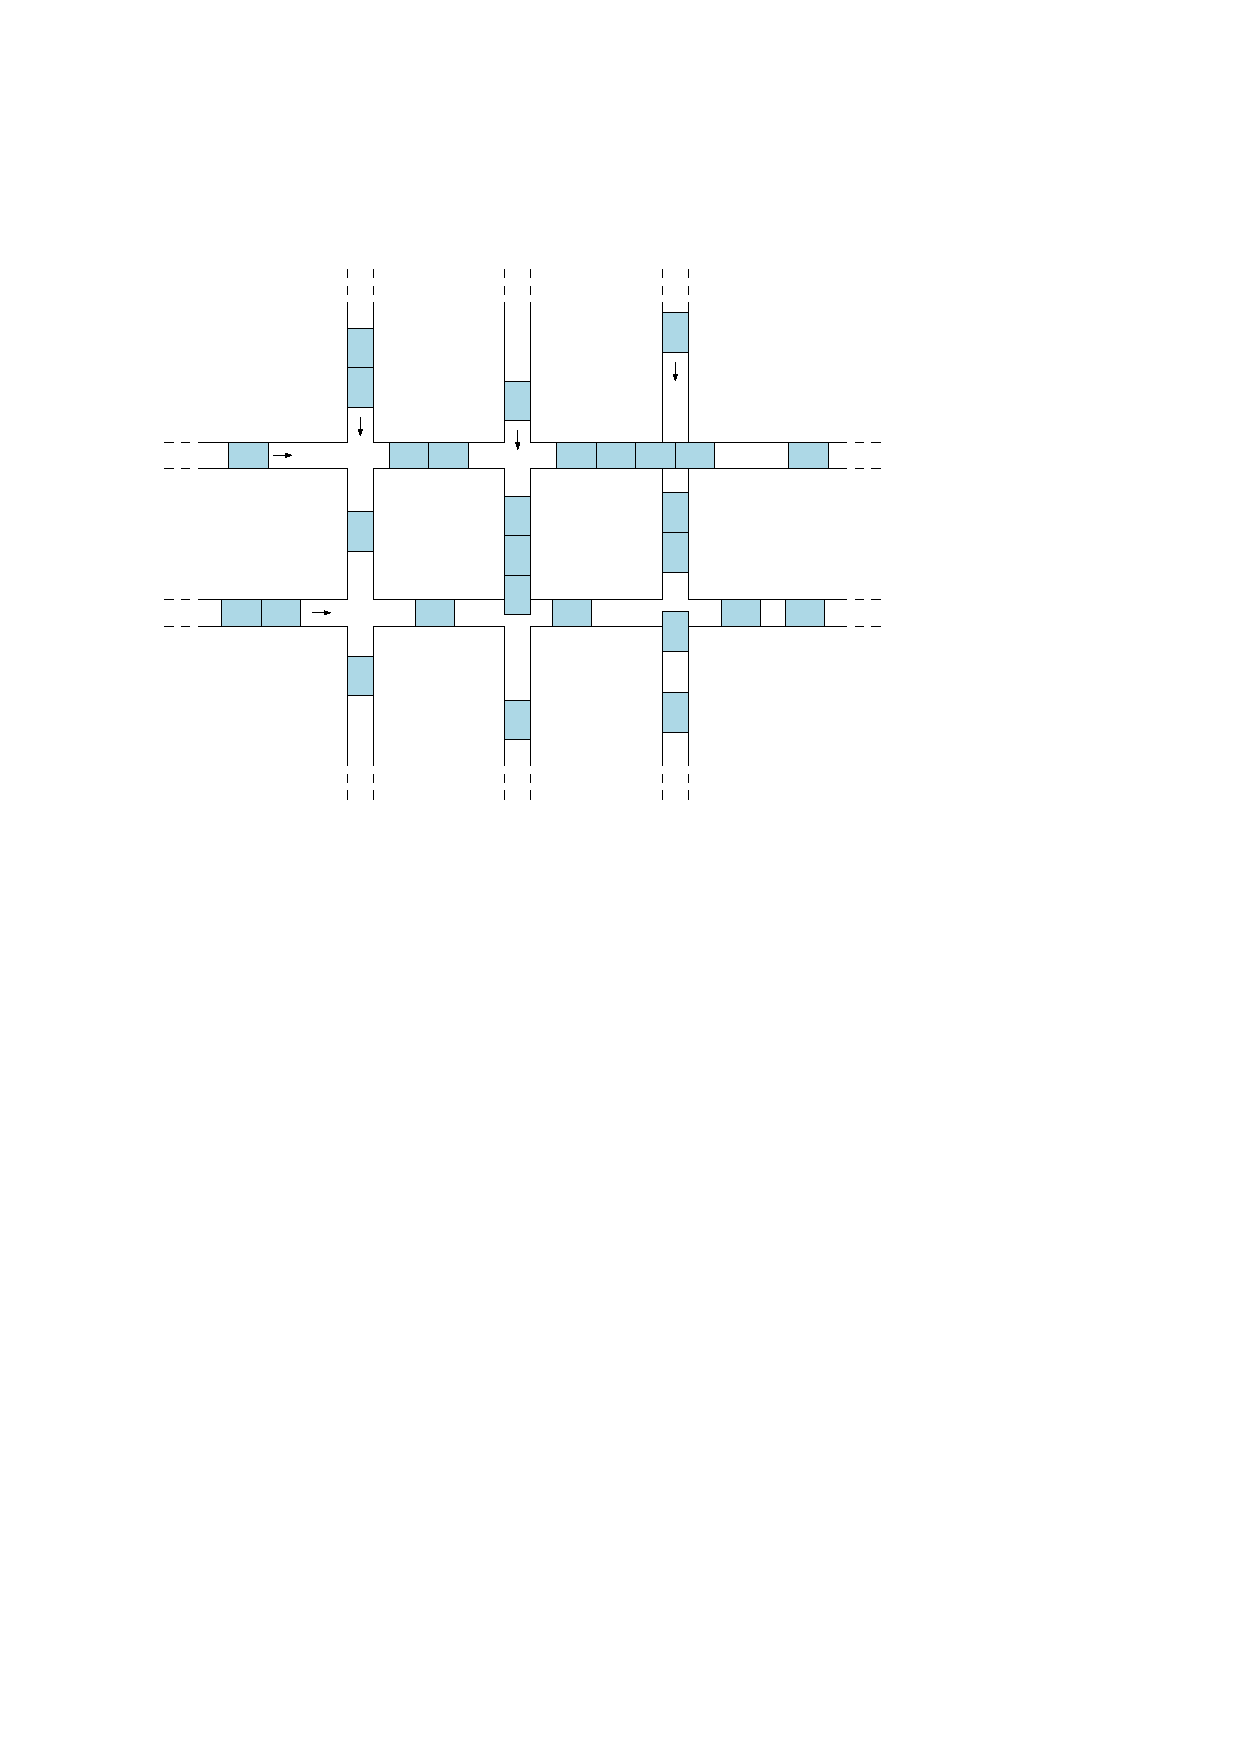
\includegraphics[scale=1]{figures/network-intersections}}
\microtypesetup{activate}
\addcontentsline{toc}{part}{Part II \;--\; Networks of Intersections}

\chapter{Learning to schedule in networks}\label{chap:network-learning}

\section{Decomposition}

Due to the second-order boundary conditions
$\dot{x}_{i}(a_{i}) = \dot{x}_{i}(b_{i}) = 1$, the feasibility of the lane
planning problem is completely characterized in terms of its schedule times.
%
We will show that it is precisely this property that us to construct a network
consisting of individual lanes, connected at intersections.
%
The fact that intersections are shared among multiple lanes naturally gives rise to some collision-avoidance constraints.
%
We will see that the feasibility of finding collision-free trajectories can be
stated completely in terms of schedule times, which essentially means that we do
not need to worry about vehicle dynamics at all.

\paragraph{Network topology.}

We will use the lane model to build a simple network model. The network model is
based on a directed graph $(\bar{V},E)$ with nodes $\bar{V}$ and arcs $E$, which
we will use to encode the possible routes.
%
Nodes with no incoming arcs are \textit{entrypoints} and nodes with no outgoing
arcs are \textit{exitpoints}.
%
We use $V$ to denote the set of \textit{intersections}, which are nodes with
in-degree at least two.
%
Let $\mathcal{R}$ denote the index set for routes, then each $r \in \mathcal{R}$
corresponds to the route
\begin{align*}
  \bar{V}_{r} = (v_{r}(0), v_{r}(1), \dots, v_{r}(m_{r}), v_{r}(m_{r}+1)) ,
\end{align*}
%
where we require $v_{r}(0)$ to be an entrypoint and $v_{r}(m_{r}+1)$ to be an
exitpoint. Furthermore, we use
$V_{r} = \bar{V}_{r} \setminus \{ v_{r}(0), \, v_{r}(m_{r}+1) \}$ to denote the
intersections on this route.
%
Let $E_{r} \subset E$ denote the set of edges that make up $V_{r}$.
%
We require that routes are \emph{edge-disjoint}, which is made precise in the
following assumption.

\begin{assump}\label{assump:disjoint-routes}
  For every distinct routes $p,q \in \mathcal{R}$ such that $p \neq q$, we
  assume $E_{p} \neq E_{q}$.
\end{assump}

This assumption ensures that each route $\bar{V}_{r}$ can be modeled by
connecting a sequence of lanes together, with some \emph{intersection areas} of
some fixed size $W$ in between them, see Figure~\ref{fig:intersections}.
%
Hence, we set the longitudinal start and end position of each lane model as
follows. Let $d(v, w)$ denote the length of edge $(v,w) \in E_{r}$, then we
recursively define
\begin{subequations}
\begin{align}
  A_{r1} &= 0 , \\
  A_{rk} &= B_{r,k-1} + W + L , \\
  B_{rk} &= A_{rk} + d(v_{r}(k-1), v_{r}(k)) ,
\end{align}
\end{subequations}
for each $k \in \{1, \dots, m_{r} + 1\}$.


\begin{figure}
  \centering
  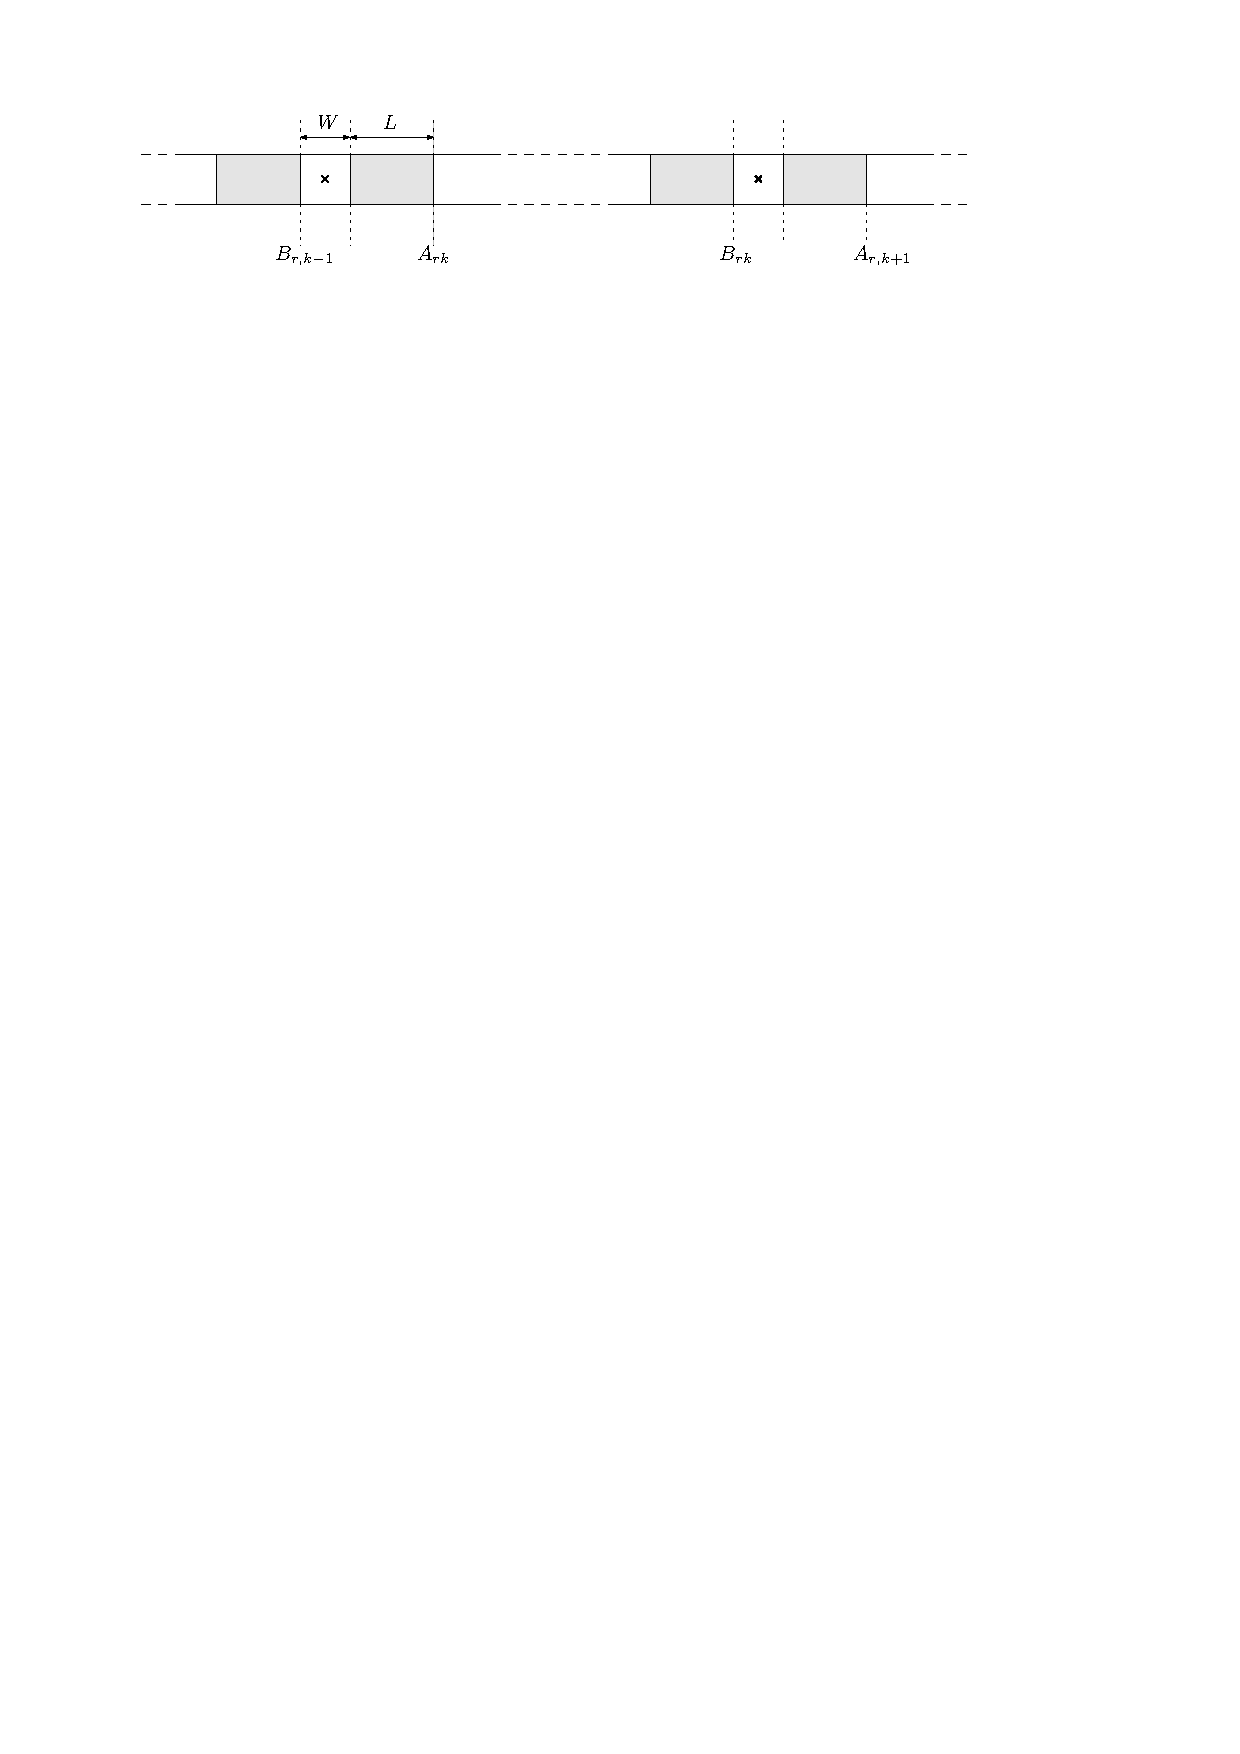
\includegraphics[scale=1]{figures/motion/intersection}
  \caption{Illustration of how the individual lane models are connected to form
    a route with intersections, marked with a little cross. The four shaded
    rectangles illustrate four possible vehicle positions. The length of the
    intersection is $W$. The longitudinal positions $A_{rk}$ and $B_{rk}$ denote
    the start and end, respectively, of the $k$th lane on route $r$.}%
  \label{fig:intersections}
\end{figure}

\paragraph{Network scheduling.}
Introduce the global trajectory planning problem by defining the
collision-avoidance constraints.
Mention that this problem can be solved at once, by using direct transcription.
%
Show that the bilevel formulation decomposes into a (combinatorial) scheduling
problem.

Assumption~\ref{assump:disjoint-routes} ensures that the order of vehicles on
each lane is completely determined by the order of vehicles on the corresponding
lane.

Instead of schedule times $a_{i}$ and $b_{i}$, we are now going to use crossing
times $y_{i}$.

Show examples of empty and full disjunctive graphs, accompanied by Gantt charts.
%
Mention that the resulting scheduling problem can be interpreted as an extension
of the classical job-shop scheduling problem.
%
Readers unfamiliar with the job shop scheduling problem may appreciate the brief introduction in Appendix~\ref{app:job-shop}.

{\color{Navy} Occupancy time slot scheduling}


\section{Notes and references}

We emphasize again that the assumption of crossing the intersection at maximum
speed is a central feature of our model, because it causes intersections to act
as a sort of ``checkpoints''.
%
The fact that the global trajectory optimization can be stated as a
jop-shop-like problem hinges on this assumption, because we essentially
``localized'' the effects of the vehicle dynamics to individual lanes; the
coupling between lanes are through the crossing times.
%
In order to relax this assumption and deal with objectives that takes into
account energy or fuel consumption, we need to take make a global trade-off
between fast crossing and energy efficiency, for which more advanced
optimization schemes are required.

Although our network examples are all grid-like and have perpendicular
intersecting lanes, the model proposed in this chapter is more generally
applicable.
%
For example, curved roads can be modeled as well, as long we assume that this
does not affect the dynamics of the vehicles, in particular the maximum speed.

\chapter{Capacitated lanes}\label{chap:network}

\note{
There is a difference in how we state the initial conditions of the system.
%
Recall that, in Chapter~\ref{chap:single}, we defined initial position
$x_{i}^{0}$ and velocity $v_{i}^{i}$ for each vehicle $i$.
This is also what is usually done when presenting an optimal control problem.
%
Instead, we now consider the time of entry into the system.
%
These two notions are not necessarily equivalent.
%
Furthermore, we need to take special care in handling the domain of the
resulting trajectories, since they are now different for each vehicle.
}

\section{Model formulation}

In our presentation of the isolated intersection model, we relied heavily on the
assumption that the intial distance to the intersection was large enough for
each vehicle to allow feasible trajectories.
%
Once we extend our model to the multi-intersection situation, it does no longer
make sense to ignore the finite length of roads between intersections. In other
words, we need to start taking into account the \emph{finite capacity} for
vehicles of each lane between intersections.
%
In order to formulate a model for a network of intersections, we first formulate
and analyze a model for such a \emph{capacitated lane}.
%
In the next chapter, we will link such lanes together to construct a model
representing a network of intersections.

We will propose a model for a one-directional single-lane road of finite length
where overtaking is not permitted.
%
The fact that such a lane can be occupied by a limited number of vehicles at the
same time, makes the characterization of set of feasible trajectories more
involved.
%
% feasibility analysis (of safe sets of trajectories)
Given some lane, consider the set of vehicles that need to travel across this
lane as part of their planned route. Suppose that the time of entry to and exit
from this lane are fixed for each of these vehicles, then the question is
whether there exists a set of trajectories that is safe, i.e., without
collisions, and which satisfies these \emph{schedule times}.
%
Loosely speaking, we ask whether there exists an easy way to answer this
feasibility question for any set of schedule times.
%
By requiring vehicles to enter and exit the lane at \emph{full speed}, we will show
that the answer positive, since the feasibility question is precisely answered
by a system of linear inequalities in terms of the schedule times.

% optimal control problem
% byproduct: algorithm for bang-bang solutions
Of course, there is generally not a single feasible set of trajectories, so we
can consider some different performance critera like we did for the isolated
intersection.
%
As we showed previously, the resulting optimal control problem is
straightforward to solve using a direct transcription method.
%
Recall the \emph{haste objective}, which seeks to minimize each vehicle's distance to
the end of the lane at all times. For this objective, we will show that the
optimal solution can be computed much more efficiently.
%
The derivation of this algorithm is a direct byproduct of the feasibility
analysis, because the latter will involve the construction of a certain set of
upper bounding trajectories, which happen to be optimal under the haste
objective.

In the remainder of this introductory section, we will precisely establish the
notion of a feasible set of trajectories in a capacitated lane. To provide some
initial intuition, we show some examples of feasible trajectories for the haste
objective.


\paragraph{Vehicle trajectories.}
We only consider the longitudinal position of vehicles on the lane and we assume
that speed and acceleration are bounded. Therefore, let $\mathcal{D}[a,b]$
denote the set of valid \emph{trajectories}, which we define to be all continuously
differentiable functions $x : [a,b] \rightarrow \mathbb{R}$ satisfying the constraints
\begin{align}
  \dot{x}(t) \in [0, 1] \quad \text{ and } \quad
  \ddot{x}(t) \in [{-\omega} ,\bar{\omega}] , \quad \text{ for all } t \in [a,b] ,
\end{align}
for some fixed acceleration bounds $\omega, \bar{\omega} > 0$ and with $\dot{x}$ and
$\ddot{x}$ denoting the first and second derivative with respect to time $t$.
Note that the unit speed upper bound is not restrictive, since we can always
apply an appropriate scaling of time and the acceleration bounds to arrive at
this form.
%
We use $A$ and $B$ to denote the start\footnote{Note that assuming $A\neq 0$ is convenient later when we start piecing together multiple lanes.} and end position of the lane.
%
Let $D_{1}[a, b] \subset \mathcal{D}[a, b]$ denote all trajectories $x$ that satisfy
the first-order boundary conditions
\begin{align}
  x(a) = A \; \text{ and } \; x(b) = B
\end{align}
and additionally satisfy $\dot{x}(a) > 0$ and $\dot{x}(b) > 0$, to avoid the
technical difficulties of dealing with vehicles that are waiting at the start or
end of the lane.
%
On top of these conditions, let $D_{2}[a,b] \subset D_{1}[a, b]$ further induce the
second-order boundary conditions
\begin{align}
  \dot{x}(a) = \dot{x}(b) = 1 .
\end{align}
In words, these boundary conditions require that a vehicle arrives to and
departs from the lane at predetermined times $a$ and $b$ and do so at full
speed.
%
Figure~\ref{fig:trajectories} shows an example for each of these three classes of trajectories.

\begin{figure}
  \centering
  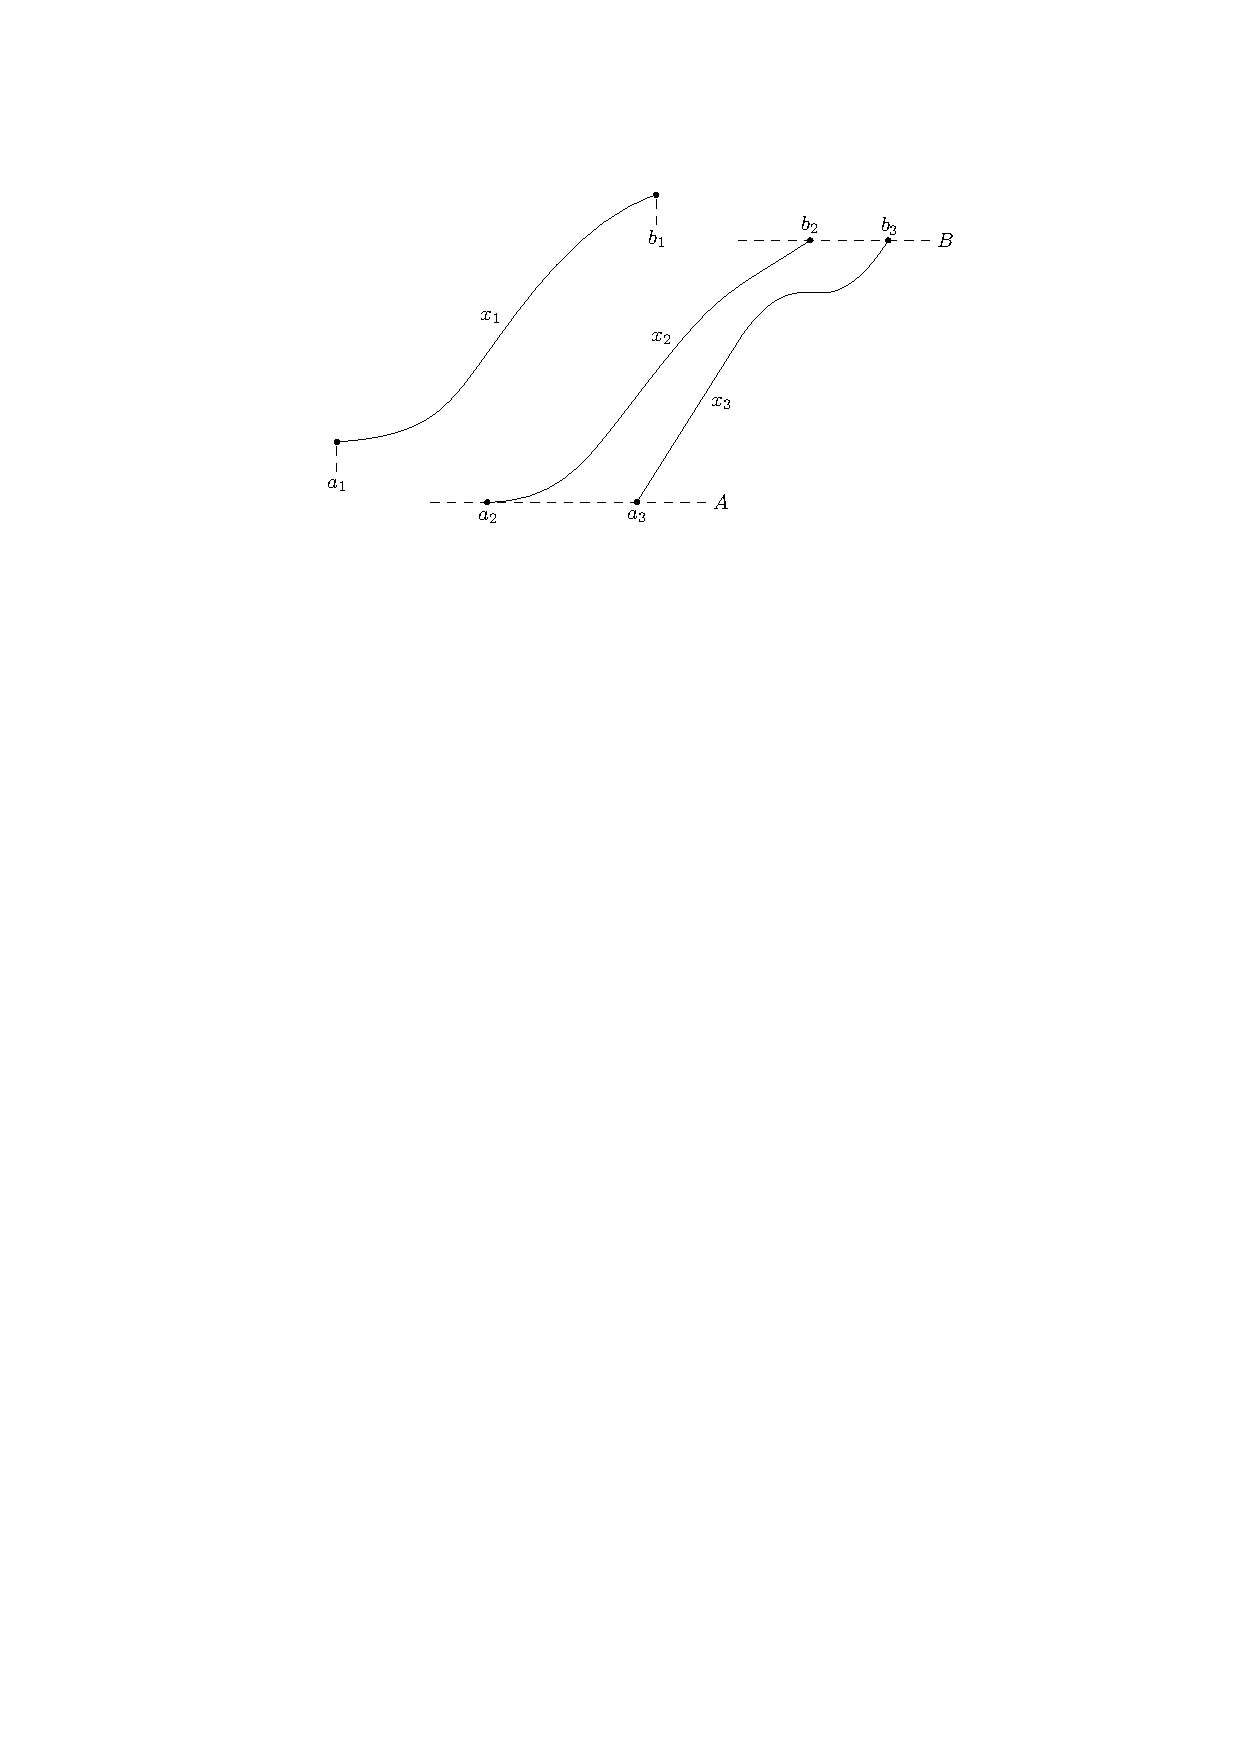
\includegraphics[scale=0.9]{figures/motion/trajectories}
  \caption{Example trajectories $x_{1} \in \mathcal{D}[a_{1},b_{1}]$,
    $x_{2} \in D_{1}[a_{2},b_{2}]$ and $x_{3} \in D_{2}[a_{3},b_{3}]$ for each
    the three classes of trajectories that are used throughout this chapter
    (horizontal axis is time, vertical axis is position).}%
  \label{fig:trajectories}
\end{figure}

\paragraph{Trajectory domains.}
Function domains will play an important role in the analysis of feasible
trajectories. Therefore, we introduce some useful notational conventions.
%
First of all, each of the trajectory classes above can be used with the common
convention of allowing $a = -\infty$ or $b = \infty$. For instance, we write
$\mathcal{D}(-\infty, \infty)$ to denote the set of trajectories defined on the
whole real line.
%
Furthermore, we use $\cdot\,|_{[a,b]}$ to denote function restriction. For example,
\begin{align*}
  (t \mapsto t + 1)|_{\halfopen{\xi}{\infty}}
\end{align*}
denotes some anonymous function with some restricted domain.
%
Furthermore, given two smooth trajectories $\gamma_{1} \in \mathcal{D}[a_{1}, b_{1}]$
and $\gamma_{2} \in \mathcal{D}[a_{2}, b_{2}]$, we write inequality
  $\gamma_{1} \preceq \gamma_{2}$ to mean
\begin{align*}
\gamma_{1}(t) \leq \gamma_{2}(t) \; \text{ for all } \; t \in [a_{1}, b_{1}] \cap [a_{2}, b_{2}] .
\end{align*}
%
Whenever the intersection of domains is empty, we say that the above inequality
is \emph{void}.
%
The reason for introducing a dedicated symbol is that $\preceq$ is not transitive.
To see this, consider the trajectories in Figure~\ref{fig:trajectories}, then
$x_{1} \preceq x_{3}$ (void) and $x_{3} \preceq x_{2}$, but clearly
$x_{1} \npreceq x_{2}$.

\begin{define}
  Let $L > 0$ denote the \textit{following distance} between consecutive vehicles.
  %
  Suppose there are $N$ vehicles scheduled to traverse the lane. For each
  vehicle $i$, let $a_{i}$ and $b_{i}$ denote the \textit{schedule time} for entry and
  exit, respectively.
  %
  Assuming that the schedule times are ordered as
  $a_{1} \leq a_{2} \leq \dots \leq a_{N}$ and
  $b_{1} \leq b_{2} \leq \dots \leq b_{N} $, then a \emph{feasible solution} consists
  of a sequence of trajectories $x_{1}, \dots, x_{N}$ such that
\begin{subequations}\label{eq:feasibility}
\begin{align}
x_{i} \in D_{2}[a_{i}, b_{i}] \quad \quad & \text{ for each } i \in \{1, \dots, N\}, \label{eq:second-order-constraint} \\
x_{i} \preceq x_{i-1} - L \quad \quad & \text{ for each } i \in \{2, \dots, N\} . \label{eq:lead-constraint}
\end{align}
\end{subequations}
We will refer to~\eqref{eq:lead-constraint} as the \emph{lead vehicle
  constraints}.
%
For some performance criterion of trajectories, given as a functional $J(x)$ of
trajectory $x$, the \emph{lane planning problem} is to find a feasible solution that
maximizes
\begin{align}\label{eq:objective}
  \min \; \sum_{i=1}^{N} J(x_{i}) .
\end{align}
\end{define}

We emphasize again that~\eqref{eq:second-order-constraint} requires vehicles to
enter and exit the lane at full speed.
%
The feasibility characterization that we will derive can now be roughly stated
as follows. Assuming the system parameters $(\omega, \bar{\omega},A,B,L)$ to be
fixed, with lane length $B-A$ sufficiently large and following distance $L$
sufficiently small, feasibility of the lane planning problem is characterized by
a system of linear inequalities in terms of the schedule times $a_{i}$ and
$b_{i}$.

\paragraph{Choice of objective.}
Recall the \emph{haste objective}, which was defined as $J_{\alpha,\beta}$ with $\alpha=-1$ and $\beta=0$, which we will from now on denote as simply
\begin{align}\label{eq:haste-objective}
  J(x_{i}) = \int_{a_{i}}^{b_{i}} - x_{i}(t) \diff t .
\end{align}
%
Roughly speaking, this objective seeks to keep all vehicles as close to the end
of the lane at all times, but it does not capture energy efficiency in any way.
%
In Section~\ref{sec:explicit-trajectories}, we will show that optimal
trajectories under the haste objective can be understood as the concatenation of
at most four different types of trajectory parts, which we might call
\emph{bang-off-bang}. Based on this observation, we present an algorithm to compute
optimal trajectories.
%
Generalizing this algorithm to other objectives like $J_{\alpha,\beta}$ with
arbitrary parameters $\alpha$ and $\beta$, is an interesting topic for further research.

% \subsection{Direct transcription}

% A straightforward way of solving
% problem~\eqref{eq:feasibility}--\eqref{eq:objective} is through direct
% transcription to a mixed-integer linear program by only considering the vehicle
% trajectories $x_{i}(t)$ at discrete time steps $t_{1}, t_{2}, \dots, t_{n}$.
% %
% We can use the forward Euler scheme to discretize the constraints.
% %
% The downside of this technique is that its computational complexity scales very
% poorly with the number of time steps.

\section{Single vehicle with arbitrary lead vehicle constraint}\label{sec:single-vehicle-problem}

Before we analyze the feasibility of the lane planning problem as a whole, we
focus on the lead vehicle constraint~\eqref{eq:lead-constraint} for a single
vehicle $i \geq 2$.
%
This allows us to lighten the notation slightly by dropping the vehicle index
$i$. Instead of $x_{i-1} - L$, we assume we are given some arbitrary \emph{lead vehicle boundary}
$u$ and consider the following problem.

\begin{define}
  Let $u \in D_{1}[c, d]$ and assume we are given two schedule times
  $a,b \in \mathbb{R}$, then the \emph{single vehicle (feasibility) problem} is to find
  a trajectory $x \in D_{2}[a,b]$ such that $x \preceq u$.
\end{define}

\subsection{Necessary conditions}

Suppose we are given some feasible trajectory $x$ for the single vehicle
problem.
%
In addition to the given upper bounding trajectory $u$, we will derive two
upper bounding trajectories $x^{1}$ and $\hat{x}$ and one lower bounding
trajectory $\check{x}$, see Figure~\ref{fig:necessary-conditions}.
%
Using these bounding trajectories, we will formulate four necessary conditions
for the single vehicle problem.

Let the \emph{full speed boundary}, denoted $x^{1}$, be defined as
\begin{align}
  x^{1}(t) = A + t - a,
\end{align}
for all $t \in [a, b]$, then we clearly have $x \preceq x^{1}$. Observe that
$x^{1}(s) = B$ for $s = a + (B-A)$, which can be interpreted as the earliest
time of departure from the lane, so we must have $b \geq a + (B-A)$. This is our
first necessary condition.
%
\begin{lemma}\label{lemma:travel-constraint}
  If there exists $x\in D_{2}[a,b]$, then $b-a \geq B-A$.
\end{lemma}

Next, since deceleration is at most $\omega$, we have
$\dot{x}(t) \geq \dot{x}(a) - \omega(t - a) = 1 - \omega(t - a)$, which we
combine with the speed constraint $\dot{x} \geq 0$ to derive
$\dot{x}(t) \geq \max\{0, 1 - \omega (t - a) \}$. Hence, we obtain the lower
bound
\begin{align}\label{eq:check-x}
  x(t) = x(a) + \int_{a}^{t} \dot{x}(\tau) \diff \tau \geq A + \int_{a}^{t} \max\{0, 1 - \omega (\tau - a) \} \diff \tau =: \check{x}(t) ,
\end{align}
for all $t \geq a$, so that we have $x \succeq \check{x}$.
%
Analogously, we derive an upper bound from the fact that acceleration is at most $\bar{\omega}$. Observe that we have
$\dot{x}(t) + \bar{\omega} (b - t) \geq \dot{x}(b) = 1$, which we combine
with the speed constraint $\dot{x}(t) \geq 0$ to derive
$\dot{x}(t) \geq \max \{ 0, 1 - \bar{\omega}(b - t) \}$. Hence, we obtain the
upper bound
\begin{align}\label{eq:hat-x}
  x(t) = x(b) - \int_{t}^{b} \dot{x}(\tau) \diff \tau
  \leq B - \int_{t}^{b} \max\{ 0, 1 -\bar{\omega} (b - \tau) \} \diff \tau =: \hat{x}(t) ,
\end{align}
for all $t \leq b$, so we have $x \preceq \hat{x}$.
%
We refer to $\check{x}$ and $\hat{x}$ as the \emph{entry boundary} and
\emph{exit boundary}, respectively.

\begin{figure}
  \centering
  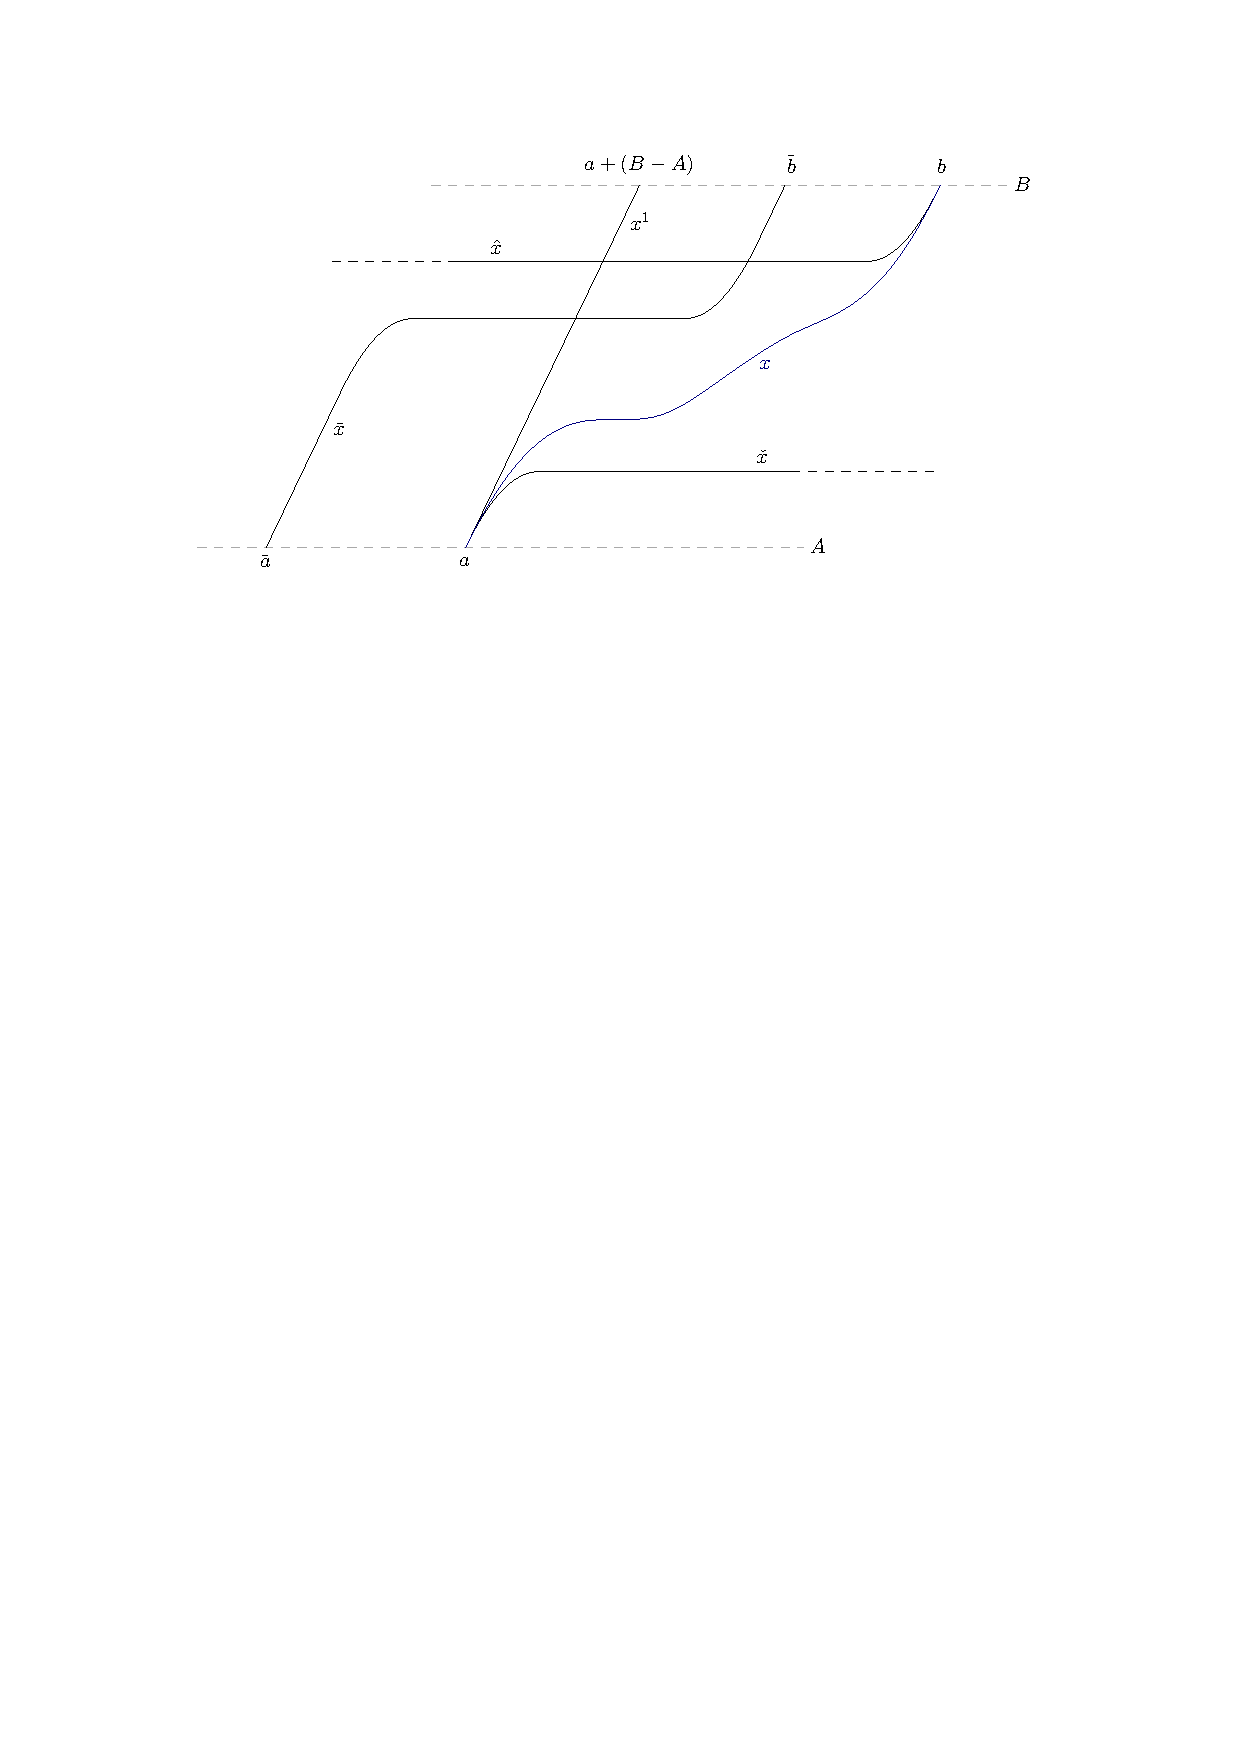
\includegraphics[scale=0.9]{figures/motion/necessary-conditions}
  \caption{Illustration of the four bounding trajectories
    $u, x^{1}, \hat{x}, \check{x}$ that bound feasible trajectories from
    above and below. We also drew an example of a feasible trajectory $x$ in
    blue. The horizontal axis represents time and the vertical axis corresponds
    to the position on the lane, so the vertical dashed grey lines correspond to
    the start and end of the lane.}%
  \label{fig:necessary-conditions}
\end{figure}

\begin{lemma}\label{lemma:necessary-conditions}
  Consider some lead boundary $u \in D_{1}[c,d]$ and assume
  $[a,b] \cap [c,d] \neq \varnothing$. If there exists a trajectory
  $x \in D_{2}[a, b]$ such that $x \preceq u$, then $a \geq c$ and $b \geq d$ and $u \succeq \check{x}$.
  % \begin{itemize}[leftmargin=3em,midpenalty=5]
  %   \item $a \geq c$,
  %   \item $b \geq d$,
  %   \item $u \succeq \check{x}$.
  % \end{itemize}
\end{lemma}
\pagebreak[1]
\begin{proof}
  Each of these conditions corresponds somehow to one of the bounding
  trajectories defined above.
  %
  Suppose $a < c$, then because the domains intersect, we must have $b > c$, but
  then clearly no $x$ can satisfy $x \preceq u$.
  %
  When $b < d$, then it is a consequence of $\dot{u}(b) > 0$ that any $x$ will
  violate $x \preceq u$.
  %
  To see that the third condition must hold, suppose that $u(\tau) < \check{x}(\tau)$
  for some time $\tau$. Since $c \leq a$, this means that $u$ must intersect
  $\check{a}$ from above. Therefore, any trajectory that satisfies $x \preceq u$
  must also intersect $\check{a}$ from above, which contradicts the assumption
  $x \in D_{2}[a,b]$.
\end{proof}

\begin{remark}
  The assumption of non-empty domains is required in the previous lemma, because
  otherwise we include the situation in which $x$ lies completely to the left of
  $u$, in which case the stated conditions are obviously not necessary anymore.
\end{remark}

We note that the boundaries $\hat{x}$ and $\check{x}$ can be combined to
yield yet another necessary condition.
%
It is straightforward to verify from~\cref{eq:hat-x,eq:check-x} that
$\hat{x}(t) \geq B - 1/(2\bar{\omega})$ and $\check{x}(t) \leq A + 1/(2\omega)$.
%
Therefore, whenever $B - A < 1/(2\bar{\omega}) + 1/(2\omega)$, these boundaries intersect
for certain values of $a$ and $b$.
%
Because the exact condition is somewhat cumbersome to characterize, we avoid
this case by simply assuming that the lane length is sufficiently large, to keep
the analysis simpler.

\begin{assump}\label{assump:lane-length}
  The length of the lane satisfies $B - A \geq 1/(2\omega) + 1/(2\bar{\omega})$.
\end{assump}

Observe that $1/(2\omega)$ is precisely the distance required to decelerate from
full speed to a standstill. Similarly, $1/(2\bar{\omega})$ is the distance
required for a full acceleration. Therefore, we may interpret
Assumption~\ref{assump:lane-length} as requiring enough space in the lane such
that there is at least one \emph{waiting position}.
%
We will return to this observation in
Section~\ref{sec:lane-problem-feasibility}.
\note{(check that we do this)}


\subsection{Sufficient conditions}\label{sec:optimal-trajectory}

\begin{figure}
  \centering
  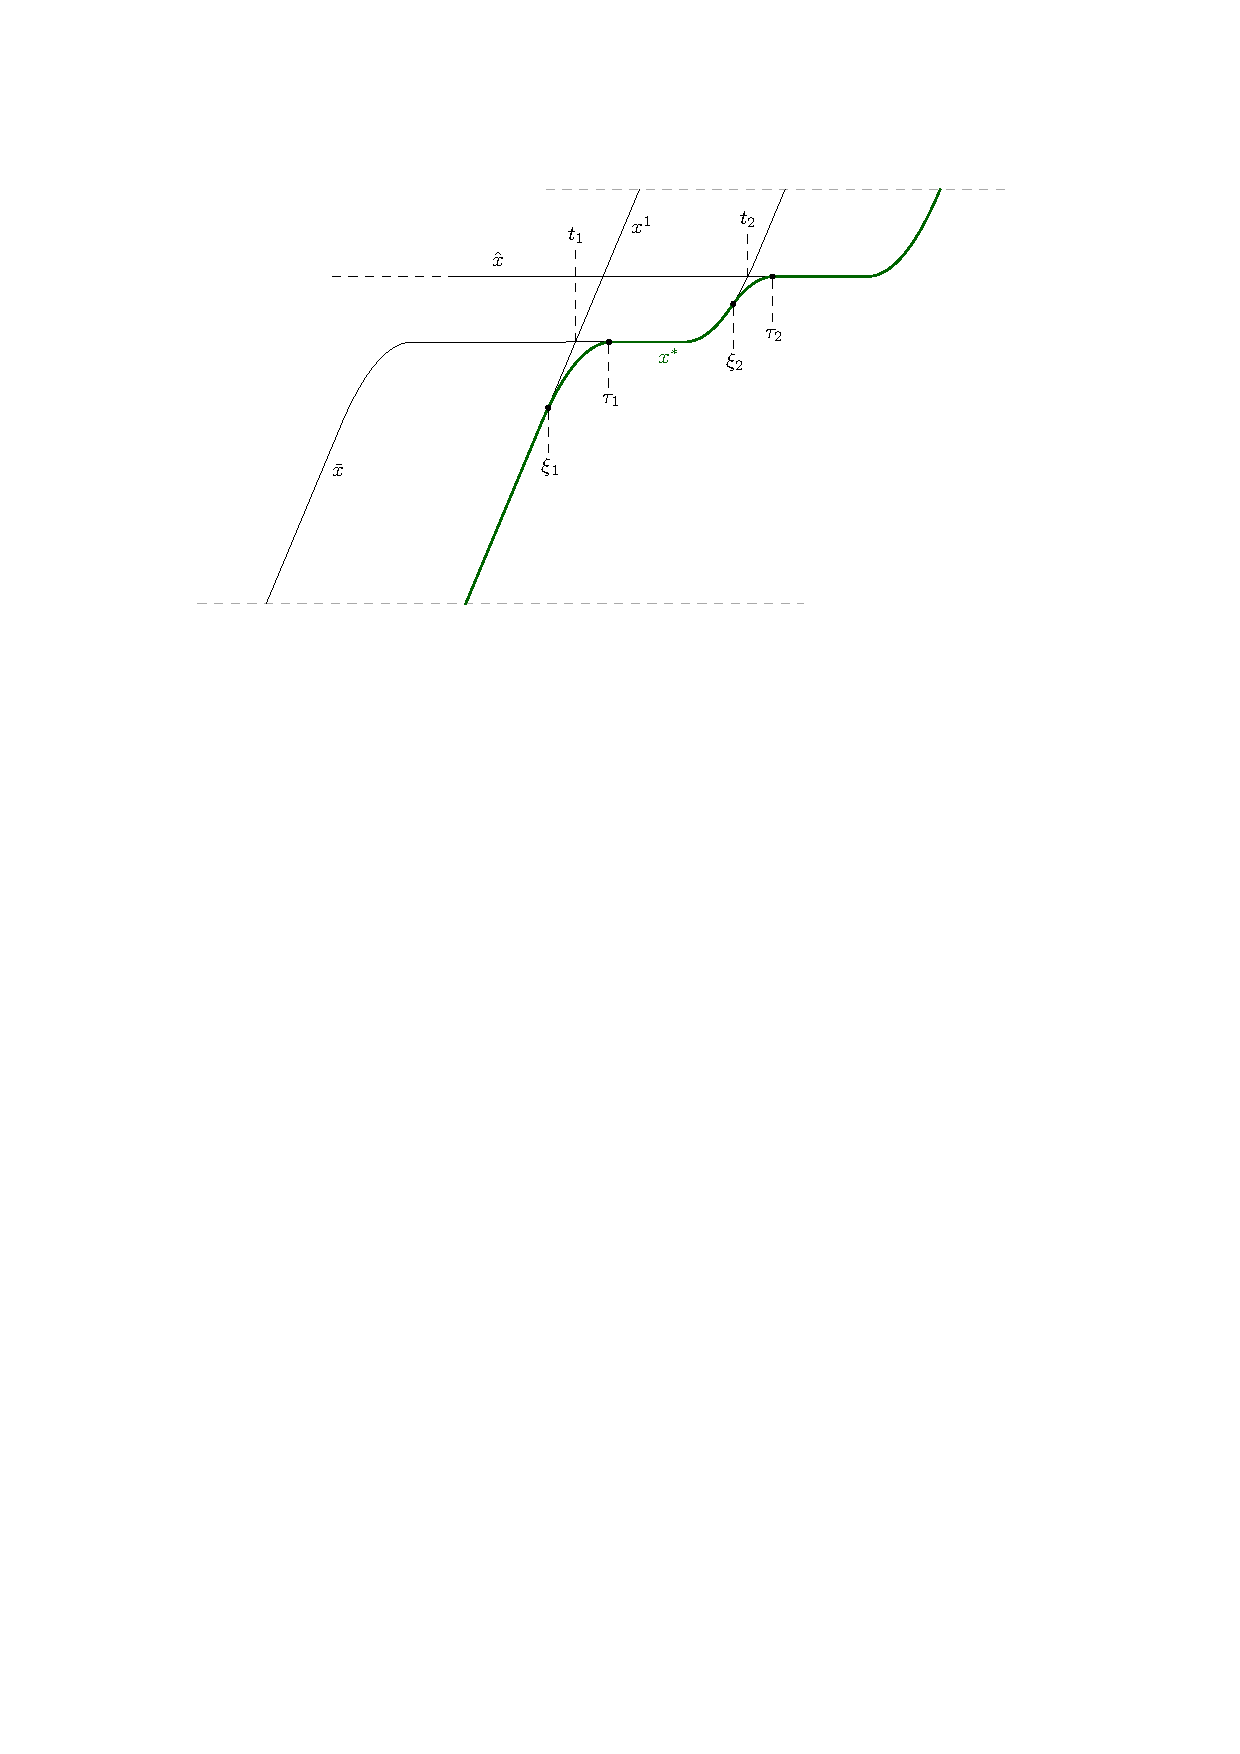
\includegraphics[scale=1]{figures/motion/proof}
  \caption{The minimum boundary $\gamma$, induced by three upper boundaries
    $u$, $\hat{x}$ and $x^{1}$, is smoothened around time $t_{1}$ and
    $t_{2}$, where the derivative is discontinuous, to obtain the smooth optimal
    trajectory $x^{*}$, drawn in green. The times $\xi_{i}$ and $\tau_{i}$
    correspond to the start and end of the connecting deceleration as
    defined in Section~\ref{sec:smoothing}.}%
  \label{fig:optimal-construction}
\end{figure}

The goal of the remainder of this section is to prove the following feasibility
characterization.

\begin{theorem}[Feasibility characterization of single vehicle
  problem]\label{thm:single-vehicle}
  Given some lead vehicle boundary $u \in D_{1}[c,d]$ and some schedule times
  $a, b \in \mathbb{R}$ such that $[a,b]\cap [c,d] \neq \varnothing$ and assuming
  Assumption~\ref{assump:lane-length}, there exists a solution
  $x \in D_{2}[a,b]$ satisfying $x \preceq u$ if and only if \TabPositions{3cm}
  \begin{enumerate}[label=(\roman*)\quad,leftmargin=5em,midpenalty=5]
    \item $b-a \geq B-A$, \tab (travel constraint)
    \item $a \geq c$, \tab (entry order constraint)
    \item $b \geq d$, \tab (exit order constraint)
    \item $u \succeq \check{x}$. \tab (entry space constraint)
  \end{enumerate}
\end{theorem}

Note that Lemma~\ref{lemma:travel-constraint} and Lemma~\ref{lemma:necessary-conditions} already showed
necessity of these conditions.
%
Therefore, we will show that, under these conditions, we can always construct a
solution $\gamma^{*}$ for the single vehicle problem, thereby showing that the
four conditions are also sufficient.
%
The particular solution that we will construct also happens to be a smooth upper
boundary for all other solutions, in the sense that, for any other feasible
solution $x$ we have $x \preceq \gamma^{*}$.
%
The starting point of the construction is the \emph{minimum boundary}
$\gamma : [a,b] \rightarrow \mathbb{R}$, defined as
\begin{align}\label{eq:min-boundary}
  \gamma(t) := \min \{ u(t), \hat{x}(t), x^{1}(t) \} .
\end{align}
%
Obviously, $\gamma$ is a valid upper boundary for any other feasible solution,
%
but in general, $\gamma$ may have a discontinuous derivative at some\footnote{In fact, it can be shown that, under the necessary conditions, there are at most two of such discontinuities.} isolated
points in time, in which case $\gamma \notin \mathcal{D}[a,b]$.

\begin{define}\label{def:piecewise-trajectory}
  Let $\mathcal{P}[a,b]$ be the set of functions $\mu : [a, b] \rightarrow \mathbb{R}$ for
  which there is a finite subdivision $a = t_{0} < \cdots < t_{n+1} = b$ such that
  the truncation $\mu|_{[t_{i}, t_{i+1}]} \in \mathcal{D}[t_{i}, t_{i+1}]$ is
  a smooth trajectory, for each $i \in \{0, \dots, n\}$, and for which the one-sided limits of $\dot{\mu}$ satisfy
  \begin{align}
    \dot{\mu}(t_{i}^{-}) := \lim_{t \uparrow t_{i}} \dot{\mu}(t) > \lim_{t \downarrow t_{i}} \dot{\mu}(t) =: \dot{\mu}(t_{i}^{+}) ,
  \end{align}
  for each $i \in \{1, \dots, n\}$. We refer to such $\mu$ as a \emph{piecewise
    trajectory (with downward bends)}.
\end{define}

Under the conditions of Theorem~\ref{thm:single-vehicle}, it is not difficult to
see from Figure~\ref{fig:necessary-conditions} that $\gamma$ satisfies the above definition, so
$\gamma \in \mathcal{P}[a,b]$. In other words, $\gamma$ consists of a number of pieces that
are smooth and satisfy the vehicle dynamics, with possibly some sharp bend
downwards where these pieces come together.
%
Next, we present a simple procedure to smoothen out this kind of discontinuity
by decelerating from the original trajectory somewhat before some $t_{i}$, as
illustrated in Figure~\ref{fig:optimal-construction}. We will argue that this procedure can be repeated as
many times as necessary to smoothen out every discontinuity.


In Section~\ref{sec:deceleration-boundary}, we first define a parameterized
family of functions to model the deceleration part that we introduce for the
smoothing procedure, which is described in Section~\ref{sec:smoothing}.
%
We apply this procedure to $\gamma$ to obtain $\gamma^{*}$, after which it is
relatively straightforward to show that $\gamma^{*}$ is an upper bound for all
other feasible solutions, which is done in
Section~\ref{sec:upper-bound-property}.


\subsection{Deceleration boundary}\label{sec:deceleration-boundary}
% In order to formalize the smoothing procedure, we will first define some
% parameterized family of functions to model the deceleration part that we
% introduce to smooth the original trajectory.
%
Recall the derivation of $\check{x}$ in equation~\eqref{eq:check-x} and the discussion
preceding it, which we will now generalize a bit.
%
Let $x \in \mathcal{D}[a, b]$ be some smooth trajectory, then observe that $\dot{x}(t) \geq \dot{x}(\xi) - \omega(t - \xi)$ for all $t \in [a, b]$.
Combining this with the constraint $\dot{x}(t) \in [0, 1]$, this yields
\begin{align}
  \dot{x}(t) \geq \max\{ 0, \, \min\{1, \, \dot{x}(\xi) - \omega (t - \xi) \}\} =: \{\dot{x}(\xi) - \omega(t-\xi)\}_{[0,1]} ,
\end{align}
where use $\{ \cdot \}_{[0,1]}$ as a shorthand for this clipping operation.
%
Hence, for any $t \in [a,b]$, we obtain the following lower bound
\begin{align}\label{eq:deceleration-boundary}
  x(t) = x(\xi) + \int_{\xi}^{t} \dot{x}(\tau) \diff \tau \geq x(\xi) + \int_{\xi}^{t} \{\dot{x}(\xi) - \omega(\tau - \xi)\}_{[0,1]} \diff \tau =: x[\xi] (t) ,
\end{align}
where we will refer to the right-hand side as the \emph{deceleration boundary} of $x$
at $\xi$.
%
Observe that this definition indeed generalizes the definition of $\check{x}$,
because we have $\check{x}=(x[a])|_{[a,b]}$.

Note that $x[\xi]$ depends on $x$ only through the two real numbers $x(\xi)$ and
$\dot{x}(\xi)$. It will be convenient later to rewrite the right-hand side
of~\eqref{eq:deceleration-boundary} as
\begin{align}\label{eq:def-x-}
  x^{-}[p, v, \xi](t) := p + \int_{\xi}^{t} \{ v - \omega(\tau - \xi) \}_{[0,1]} \diff \tau ,
\end{align}
such that $x[\xi](t) = x^{-}[x(\xi), \dot{x}(\xi), \xi](t)$.
%
We can expand the integral in this expression further by carefully handling the
clipping operation. Observe that the expression within the clipping operation
reaches the bounds $1$ and $0$ for $\delta_{1} := \xi - (1-v)/\omega$ and
$\delta_{0} := \xi + v/\omega$, respectively. Using this notation, a straightforward
calculation shows that
\begin{align}\label{eq:x-}
  x^{-}[p,v,\xi](t) = p +
  \begin{cases}
    {(1 - v)}^{2} / (2\omega) + (t - \xi) & \text{ for } t \leq \delta_{1} , \\
    v(t - \xi) - \omega{(t-\xi)}^{2} /2 & \text{ for } t \in [\delta_{1} , \delta_{0}] , \\
    v^{2}/(2\omega) & \text{ for } t \geq \delta_{0} .
  \end{cases}
\end{align}
%
It is easily verified that the three cases above coincide at
$t \in \{\delta_{1}, \delta_{0}\}$, which justifies the overlaps in the case distinction.
Furthermore, since $x$ and $\dot{x}$ are continuous by assumption, it follows
that $x[\xi](t) = x^{-}[x(\xi), \dot{x}(\xi), \xi](t)$ is continuous as a function of
either of its arguments.\footnote{Even more, it can be shown that $x[\xi](t)$ is continuous as a function of $(\xi, t)$.}
%
Assuming $0 \leq v \leq 1$, it can be verified that for every $t \in \mathbb{R}$, we
have $\ddot{x}^{-}[p,v,\xi](t) \in \{-\omega, 0\}$ and
$\dot{x}^{-}[p,v,\xi](t) \in [0,1]$ due to the clipping operation, so that
$x^{-}[p,v,\xi] \in \mathcal{D}(-\infty,\infty)$.

\begin{figure}
  \centering
  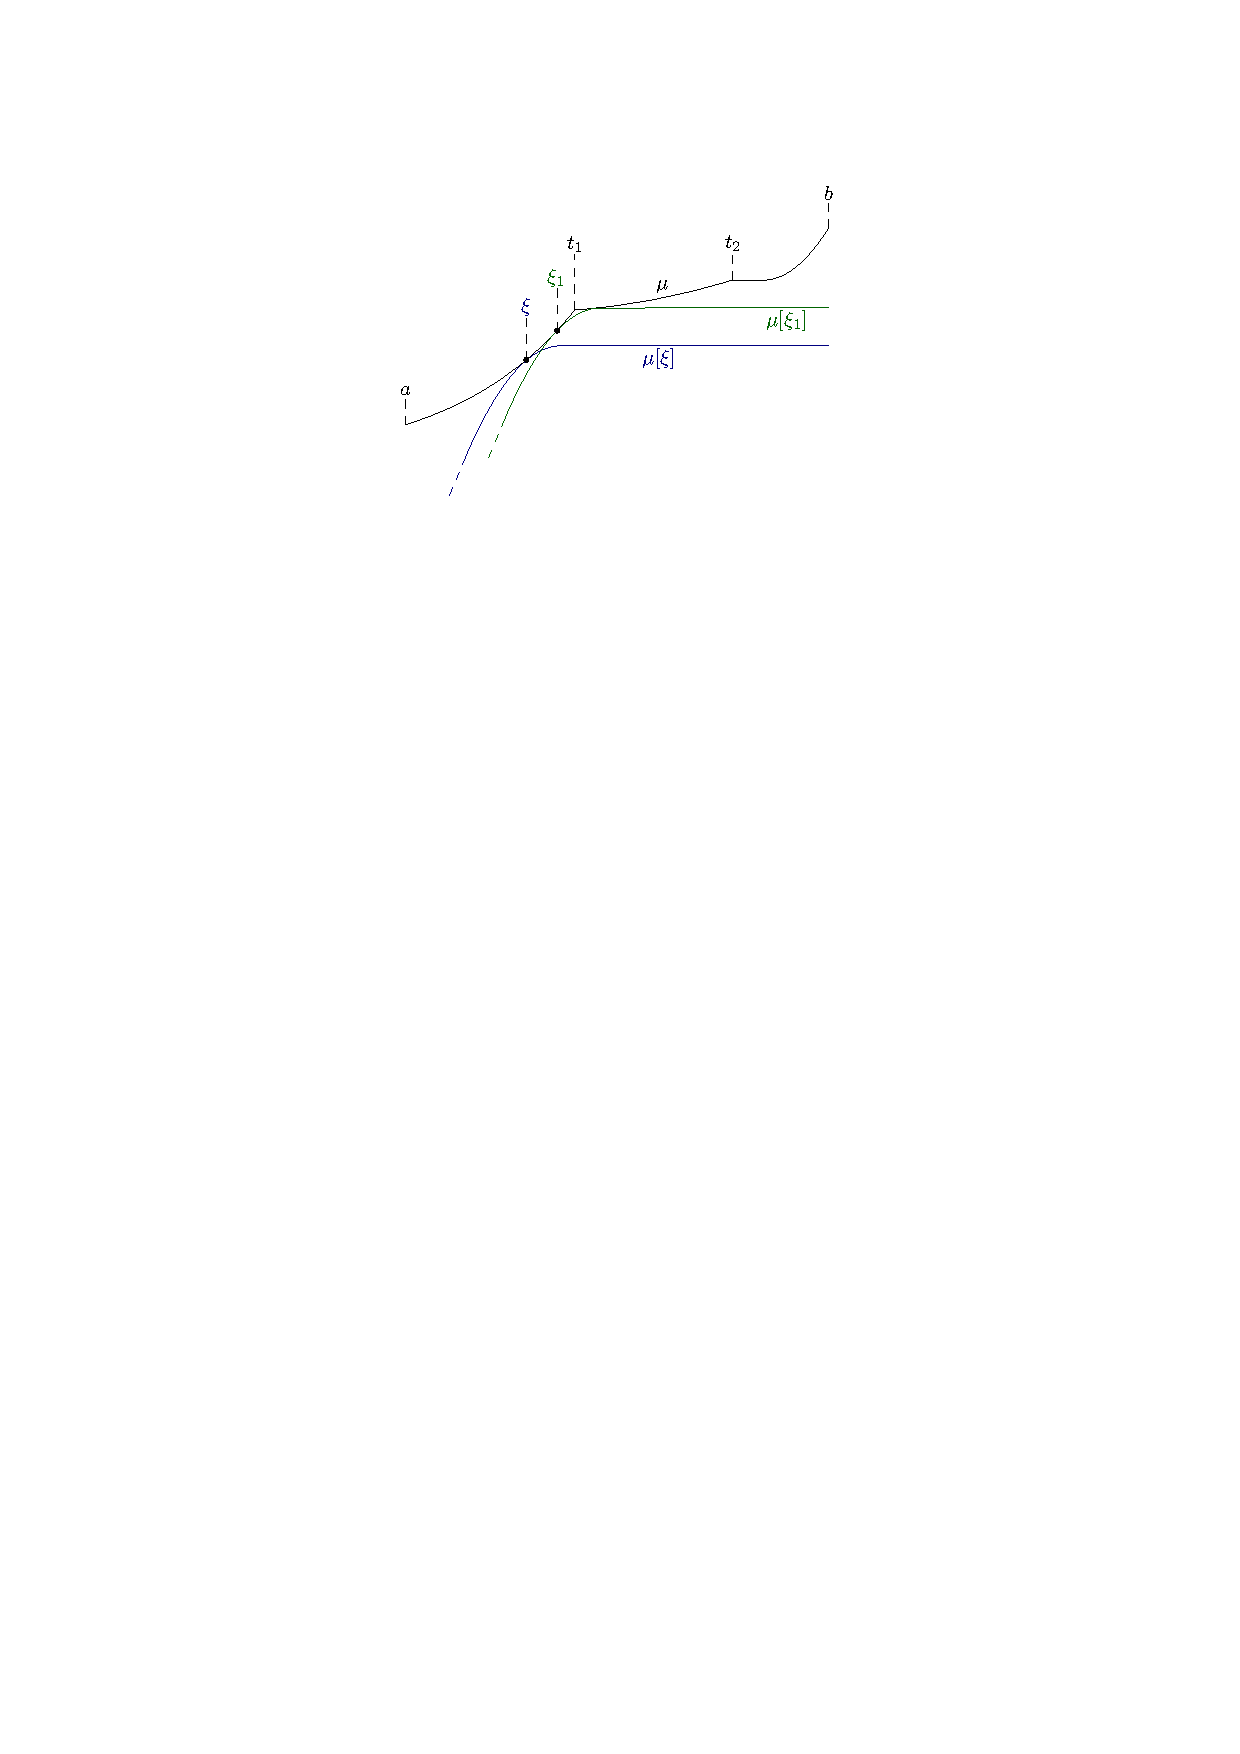
\includegraphics[scale=1.1]{figures/motion/deceleration-boundary}
  \caption{Illustration of some piecewise trajectory $\mu \in \mathcal{P}[a,b]$ with
    a discontinuous derivative at times $t_{1}$ and $t_{2}$. Furthermore, the
    figure shows some arbitrary deceleration boundary $\mu[\xi]$ at time $\xi$ in blue
    and the unique connecting deceleration $\mu[\xi_{1}]$ to the cover discontinuity at
    $t_{1}$ in green. We truncated the start of both deceleration boundaries for
    a more compact figure. The careful observer may notice that $\mu$ cannot occur
    as the minimum boundary defined in~\eqref{eq:min-boundary}, but please note that the class of
    piecewise trajectories $\mathcal{P}[a,b]$ is just slightly more general than
    necessary for our current purposes.}%
  \label{fig:deceleration-boundary}
\end{figure}


\paragraph{Piecewise trajectories.}
Let $\mu \in \mathcal{P}[a, b]$ be some piecewise trajectory with corresponding
subdivision $a = t_{0} < \cdots < t_{n+1} = b$ as defined in Definition~\ref{def:piecewise-trajectory}. It is
straightforward to generalize the definition of a deceleration boundary to $\mu$.
%
Whenever $\xi \in [a,b] \setminus \{ t_{1}, \dots, t_{n}\}$, we just define
$\mu[\xi] := x^{-}[\mu(\xi), \dot{\mu}(\xi), \xi]$, exactly like we did for $x$.
%
However, at the points of discontinuity $\xi \in \{ t_{1}, \dots, t_{n}\}$, the
derivative $\dot{\mu}(\xi)$ is not defined, so we choose to use the left-sided limit
instead, by defining $\mu[\xi] := x^{-}[\mu(\xi), \dot{\mu}(\xi^{-}), \xi]$.

\begin{remark}\label{rem:lower-bound-piecewise}
  Please note that we cannot just replace $x$ with $\mu$ in inequality~\eqref{eq:deceleration-boundary} to
  obtain a similar bound for $\mu$ on the its full interval $[a,b]$.
  Instead, we get the following \emph{piecewise lower bounding} property.
  %
  Consider some interval
  $I \in \{ [a, t_{1}], \openhalf{t_{1}}{t_{2}}, \dots, \openhalf{t_{n}}{b} \}$, then what
  remains true is that $\xi \in I$ implies $\mu(t) \geq \mu[\xi](t)$ for every $t \in I$.
\end{remark}


\subsection{Smoothing procedure}\label{sec:smoothing}
Let $\mu \in \mathcal{P}[a,b]$ be some piecewise trajectory and let
$a = t_{0} < \cdots < t_{n+1} = b$ denote the subdivision as in Definition~\ref{def:piecewise-trajectory}.
%
We first show how to smoothen the discontinuity at $t_{1}$ and then argue how to
repeat this process for the remaining times $t_{i}$.
Our aim is to choose some time $\xi \in [a,t_{1}]$ from which the vehicle starts
fully decelerating, such that $\mu[\xi] \preceq \mu$ and such that $\mu[\xi]$ touches $\mu$ at some time
$\tau \in [t_{1}, b]$ tangentially.
%
We will show there is a unique trajectory $\mu[\xi]$ that satisfies these requirements
and refer to it as the \emph{connecting deceleration}, see
Figure~\ref{fig:deceleration-boundary} for an example.
%
The construction relies on the following technical assumption.

\begin{assump}\label{assump:smoothing}
  Throughout the following discussion, we assume $\mu \succeq \mu[a]$ and $\mu \succeq \mu[b]$.
\end{assump}



\paragraph{Touching.}
Recall Remark~\ref{rem:lower-bound-piecewise}, which asserts that we have
$\mu[\xi](t) \leq \mu(t)$ for every $t \in [a,t_{1}]$ for any $\xi \in [a, t_{1}]$.
%
After the discontinuity, so for every $t \in [t_{1}, b]$, we want
$\mu[\xi](t) \leq \mu(t)$ and equality at least somewhere, so we measure the relative
position of $\mu[\xi]$ with respect to $\mu$ here, by considering
\begin{align}
  d(\xi) := \min_{t \in [t_{1}, b]} \mu(t) - \mu[\xi](t) .
\end{align}
Since $\mu(t)$ and $\mu[\xi](t)$ are both continuous as a function of $t$ on the interval
$[t_{1}, b]$, this minimum actually exists (extreme value theorem).
%
Furthermore, since $d$ is the minimum of a continuous function over a closed
interval, it is continuous as well (see Lemma~\ref{lemma:inf-continuous}).
%
Observe that $d(a) \geq 0$, because $\mu \succeq \mu[a]$ by Assumption~\ref{assump:smoothing}.
%
By definition of $t_{1}$, we have $\dot{\mu}(t_{1}^{-}) > \dot{\mu}(t_{1}^{+})$,
from which it follows that $\mu(t) < \mu[t_{1}](t)$ for $ t\in (t_{1}, t_{1} + \epsilon)$ for some
small $\epsilon > 0$, which shows that $d(t_{1}) < 0$.
%
By the intermediate value theorem, there is $\xi_{1} \in \halfopen{a}{t_{1}}$ such
that $d(\xi_{1}) = 0$.
%
This shows that $\mu[\xi_{1}]$ touches $\mu$ at some time
$\tau_{1} \in [t_{1}, b]$.


\paragraph{Uniqueness.}
It turns out that $\xi_{1}$ itself is not necessarily unique, which we explain
below. Instead, we are going to show that the connecting deceleration
$\mu[\xi_{1}]$ is unique. More precisely, given any other $\xi \in \halfopen{a}{t_{1}}$ such
that $d(\xi) = 0$, we will show that $\mu[\xi] = \mu[\xi_{1}]$.

The first step is to establish that the level set
\begin{align}
  X := \{ \xi \in \halfopen{a}{t_{1}} : d(\xi) = 0 \}
\end{align}
is a closed interval. To this end, we show that $d$ is non-increasing on
$\halfopen{a}{t_{1}}$, which together with continuity implies the desired result
(see Lemma~\ref{lemma:levelset}).
%
To show that $d$ is non-increasing, it suffices to show that $\mu[\xi](t)$ is
non-decreasing as a function of $\xi$, for every $t \in [t_{1}, b]$.
%
We can do this by computing the partial derivative of $\mu[\xi]$ with respect to $\xi$
and verifying it is non-negativity.
%
Recall the definition of $\mu[\xi]$, based on $x^{-}$ in equation~\eqref{eq:x-}.
%
Using similar notation, we write
$\delta_{1}(\xi) = \xi - (1 - \dot{\mu}(\xi))/\omega$ and
$\delta_{0}(\xi) = \xi + \dot{\mu}(\xi)/\omega$ and compute
%
\begin{align}
  \frac{\partial}{\partial \xi} \mu[\xi](t) =
  \dot{\mu}(\xi) +
  \begin{cases}
    \ddot{\mu}(\xi)(\dot{\mu}(\xi)-1)/\omega - 1 &\text{ for } t \leq \delta_{1}(\xi) , \\
    \ddot{\mu}(\xi)(t-\xi) - \dot{\mu}(\xi) + \omega(t-\xi) &\text{ for } t \in [\delta_{1}(\xi),\delta_{0}(\xi)] , \\
    \ddot{\mu}(\xi)\dot{\mu}(\xi)/ \omega &\text{ for } t \geq \delta_{0}(\xi) .
  \end{cases}
\end{align}
%
It is easily verified that the cases match at
$t \in \{\delta_{1}(\xi), \delta_{0}(\xi)\}$, which justifies the overlaps there.
%
Consider any $\xi \in \halfopen{a}{t_{1}}$ and $t \in [t_{1}, b]$, then we always have
$\delta_{1}(\xi) \leq \xi \leq t$, so we only have to verify the second and third case:
%
\begin{subequations}
\begin{alignat}{2}
  \frac{\partial}{\partial \xi} \mu[\xi](t) &= (\ddot{\mu}(\xi) + \omega)(t-\xi) \geq 0 \quad\quad\quad &&\text{ for } t \in [\delta_{1}(\xi) ,\delta_{0}(\xi)], \label{eq:case2} \\
  \frac{\partial}{\partial \xi} \mu[\xi](t) &\geq \dot{\mu}(\xi) + (-\omega)\dot{\mu}(\xi)/\omega = 0 &&\text{ for } t \geq \delta_{0}(\xi) . \label{eq:case3}
\end{alignat}
\end{subequations}
%
This concludes the argument for $X$ being a closed interval.

Assuming $\xi$ to be fixed, observe that there is equality in~\eqref{eq:case2} for some
$t \in [\delta_{1}(\xi), \delta_{0}(\xi)]$ if and only if there is equality in~\eqref{eq:case3}
for some other $t' \geq \delta_{0}(\xi)$. Note that this happens precisely when
$\ddot{\mu}(\xi) = -\omega$.
%
Therefore, whenever $\mu$ is fully deceleration, so $\dot{\mu}(t)=-\omega$ on
some open interval $U \subset (a, t_{1})$, we have
$(\partial/\partial \xi) \mu[\xi](t) = 0$ for all $t \geq \delta_{1}(\xi)$.
%
This essentially means that any choice of $\xi \in U$ produces the same
trajectory $\mu[\xi]$. Please see Figure~\ref{fig:deceleration-boundary-unique}
for an example of this case.
%
This observation is key to the remaining uniqueness argument.

\begin{figure}[h]
  \centering
  \vspace*{0.5em}
  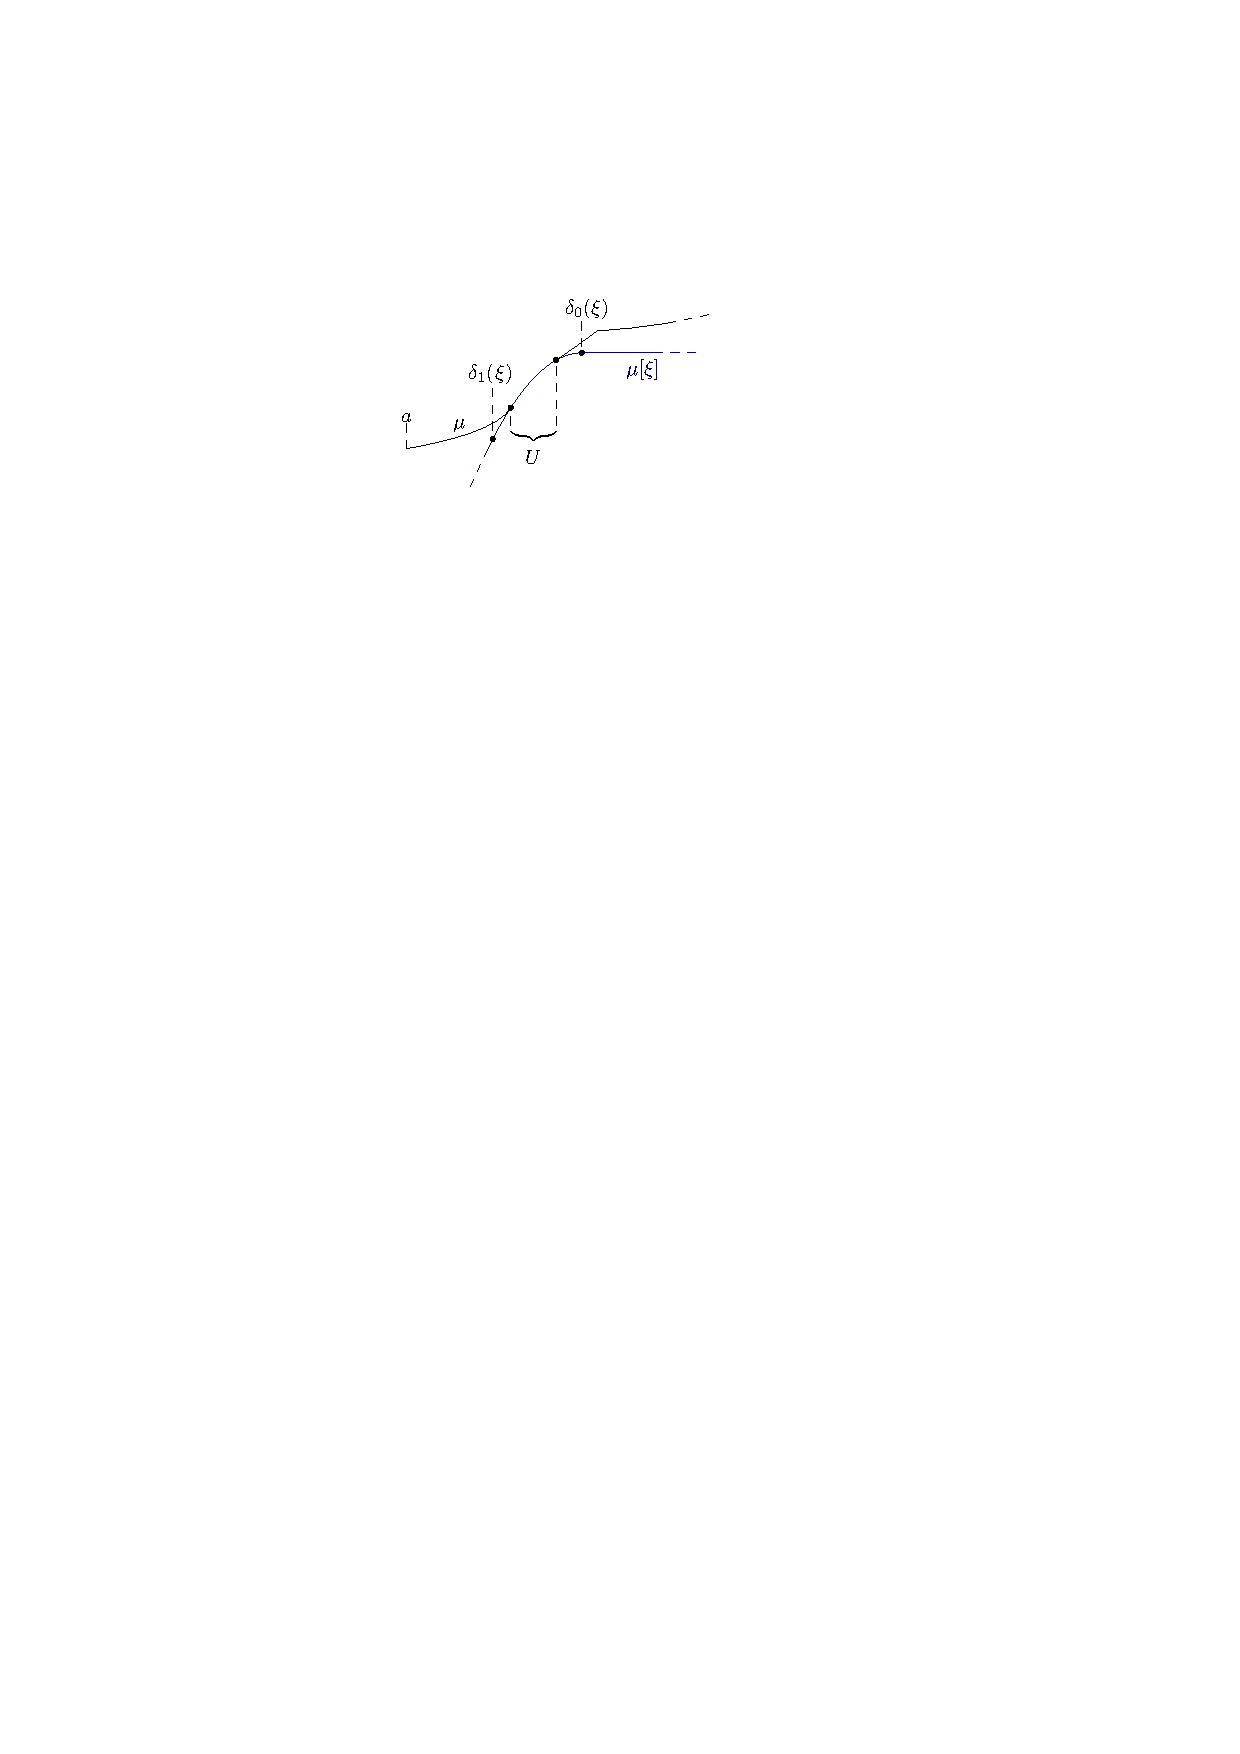
\includegraphics[scale=1.1]{figures/motion/deceleration-boundary-unique}
  \caption{Example of a piecewise trajectory $\mu$ with a part of full
    deceleration over some interval $U$ such that any choice of $\xi \in U$
    produces the same deceleration boundary $\mu[\xi]$, which naturally
    coincides with $\mu$ on $U$.}
  \label{fig:deceleration-boundary-unique}
\end{figure}

Since $X$ is a closed interval, we may define $\xi_{0} = \min X$.
%
Consider any $\xi' \in X$ with $\xi' > \xi_{0}$, then we show $\mu[\xi'](t) = \mu[\xi_{0}](t)$ for all
$t \in [\xi_{0}, b]$. For sake of contradiction, suppose there is some $t' \in [\xi_{0}, b]$ such that
$\mu[\xi'](t') > \mu[\xi_{0}](t')$, then there must be some open interval $U \subset (\xi_{0}, \xi')$ such that
\begin{align}\label{eq:positive-partial-derivative}
  \frac{\partial}{\partial \xi}\mu[\xi](t') > 0 \text{ for all } \xi \in U .
\end{align}
However, we argued in the previous paragraph that this actually holds for any
$t' \geq \delta_{1}(\xi)$.
%
In particular, let $t^{*} \in [t_{1}, b]$ be such that
$\mu(t^{*}) = \mu[\xi_{0}](t^{*})$, then
$t^{*} \geq t_{1} \geq \xi \geq \delta_{1}(\xi)$,
so~\eqref{eq:positive-partial-derivative} yields $\mu[\xi'](t^{*}) > \mu[\xi_{0}](t^{*})$, but then
$d(\xi') > d(\xi_{0}) = 0$, so $\xi' \notin X$, a contradiction.


\paragraph{Touching tangentially.}
\comment{I might add a figure for this whole part. Especially for the case tau1
  = b, because feasibility of the resulting trajectory relies on this.}
%
It remains to show that $\mu$ and $\mu[\xi_{0}]$ touch tangentially somewhere on
$[t_{1}, b]$. Let $\tau_{1} \in [t_{1}, b]$ be the smallest time such that
$\mu(\tau_{1}) - \mu[\xi_{0}](\tau_{1}) = d(\xi_{0}) = 0$ and consider the
following three cases.

First of all, note that $\tau_{1} = t_{1}$ is not possible, because this
would require
\begin{align}
  \dot{\mu}(t_{1}^{+}) > \dot{\mu}[\xi_{0}](t_{1}^{+}) = \dot{\mu}[\xi_{0}](t_{1}) ,
\end{align}
but since $\mu$ is a piecewise trajectory, we must have
$\dot{\mu}(t_{1}^{-}) > \dot{\mu}(t_{1}^{+}) > \dot{\mu}[\xi_{0}](t_{1})$. This
shows that $\mu(t_{1} - \epsilon) < \mu[\xi_{0}](t_{1} - \epsilon)$, for
some small $\epsilon > 0$, which contradicts $\mu[\xi_{0}] \preceq \mu$.

Suppose $\tau_{1} \in (t_{1}, b)$, then recall the definition of $d(\xi_{0})$
and observe that the usual first-order necessary condition (derivative zero) for
local minima requires $\dot{\mu}(\tau_{1}) = \dot{\mu}[\xi_{0}](\tau_{1})$.
\comment{I find this argument clear enough, but I am not sure if
  ''first-order necessary condition'', needs some further elaboration. It is
  just when you are minimizing some differentiable function f(x), then a local
  minimum a should have f'(a) = 0.}

Finally, consider $\tau_{1} = b$.
%
Observe that $\dot{\mu}(b) > \dot{\mu}[\xi_{0}](b)$, would contradict
minimality of $\tau_{1} = b$. Therefore, suppose
$\dot{\mu}(b) < \dot{\mu}[\xi_{0}](b)$, then
$\dot{\mu}[b](b) = \dot{\mu}(b) < \dot{\mu}[\xi_{0}](b)$, so
\begin{align}
  \dot{\mu}[b](t) \leq \dot{\mu}[\xi_{0}](t) \text{ for } t \leq b ,
\end{align}
but then $\mu[b](t) > \mu[\xi_{0}](t)$ for $t < b$. In particular, for $t=\xi_{0}$, this shows
$\mu[b](\xi_{0}) > \mu[\xi_{0}](\xi_{0}) = \mu(\xi_{0})$, which contradicts part $\mu[b] \preceq \mu$ of
Assumption~\ref{assump:smoothing}.


\paragraph{Repeat for remaining discontinuities.}
Let us summarize what we have established so far.
%
The times $\xi_{0} \in \halfopen{a}{t_{1}}$ and
$\tau_{1} \in \openhalf{t_{1}}{b}$ have been chosen such that
\begin{subequations}\label{eq:smoothing-requirements}
\begin{gather}
  \mu[\xi_{0}](t) \leq \mu(t) \; \text{ for } \; t \in [\xi_{0}, \tau_{1}] , \\
  \dot{\mu}[\xi_{0}](\xi_{0}) = \dot{\mu}(\xi_{0}) \; \text{ and } \; \dot{\mu}[\xi_{0}](\tau_{1}) = \dot{\mu}(\tau_{1}) .
\end{gather}
\end{subequations}
Instead of $\xi_{0}$, it will be convenient later to choose $\xi_{1} := \max X$
as the representative of the unique connecting deceleration.
%
We can now use $(\mu[\xi_{1}])|_{[\xi_{1},\tau_{1}]}$ to replace $\mu$ at $[\xi_{1}, \tau_{1}]$ to
obtain a trajectory without the discontinuity at $t_{1}$. More precisely, we
define
\begin{align}
  \mu_{1}(t) =
  \begin{cases}
    \mu(t) &\text{ for } t \in [a, \xi_{1}] \cup [\tau_{1}, b] , \\
    \mu[\xi_{1}](t) &\text{ for } t \in [\xi_{1}, \tau_{1}] .
  \end{cases}
\end{align}
From the way we constructed $\mu[\xi_{1}]$, it follows
from~\eqref{eq:smoothing-requirements} that we have
$\mu_{1} \in \mathcal{P}[a,b]$, but without the discontinuity at $t_{1}$.
%
Observe that a single connecting deceleration may cover more than one
discontinuity, as illustrated in Figure~\ref{fig:multiple-discontinuities}.
%
Note that we must have $\dot{\mu}_{1}(a) = \dot{\mu}(a)$ and
$\dot{\mu}_{1}(b) = \dot{\mu}(b)$ by construction.
%
Hence, it is not difficult to see that $\mu_{1}$ must still satisfy
Assumption~\ref{assump:smoothing}, so that we can keep repeating the exact same
process, obtaining connecting decelerations $(\xi_{2}, \tau_2), (\xi_{3}, \tau_{3}), \,\dots$
and the corresponding piecewise trajectories $\mu_{2}, \mu_{3}, \,\dots$ to remove any
remaining discontinuities until we end up with a smooth trajectory
$\mu^{*} \in \mathcal{D}[a,b]$.
%
We emphasize again that $\dot{\mu}^{*}(a) = \dot{\mu}(a)$ and
$\dot{\mu}^{*}(b) = \dot{\mu}(b)$.

\begin{figure}
  \centering
  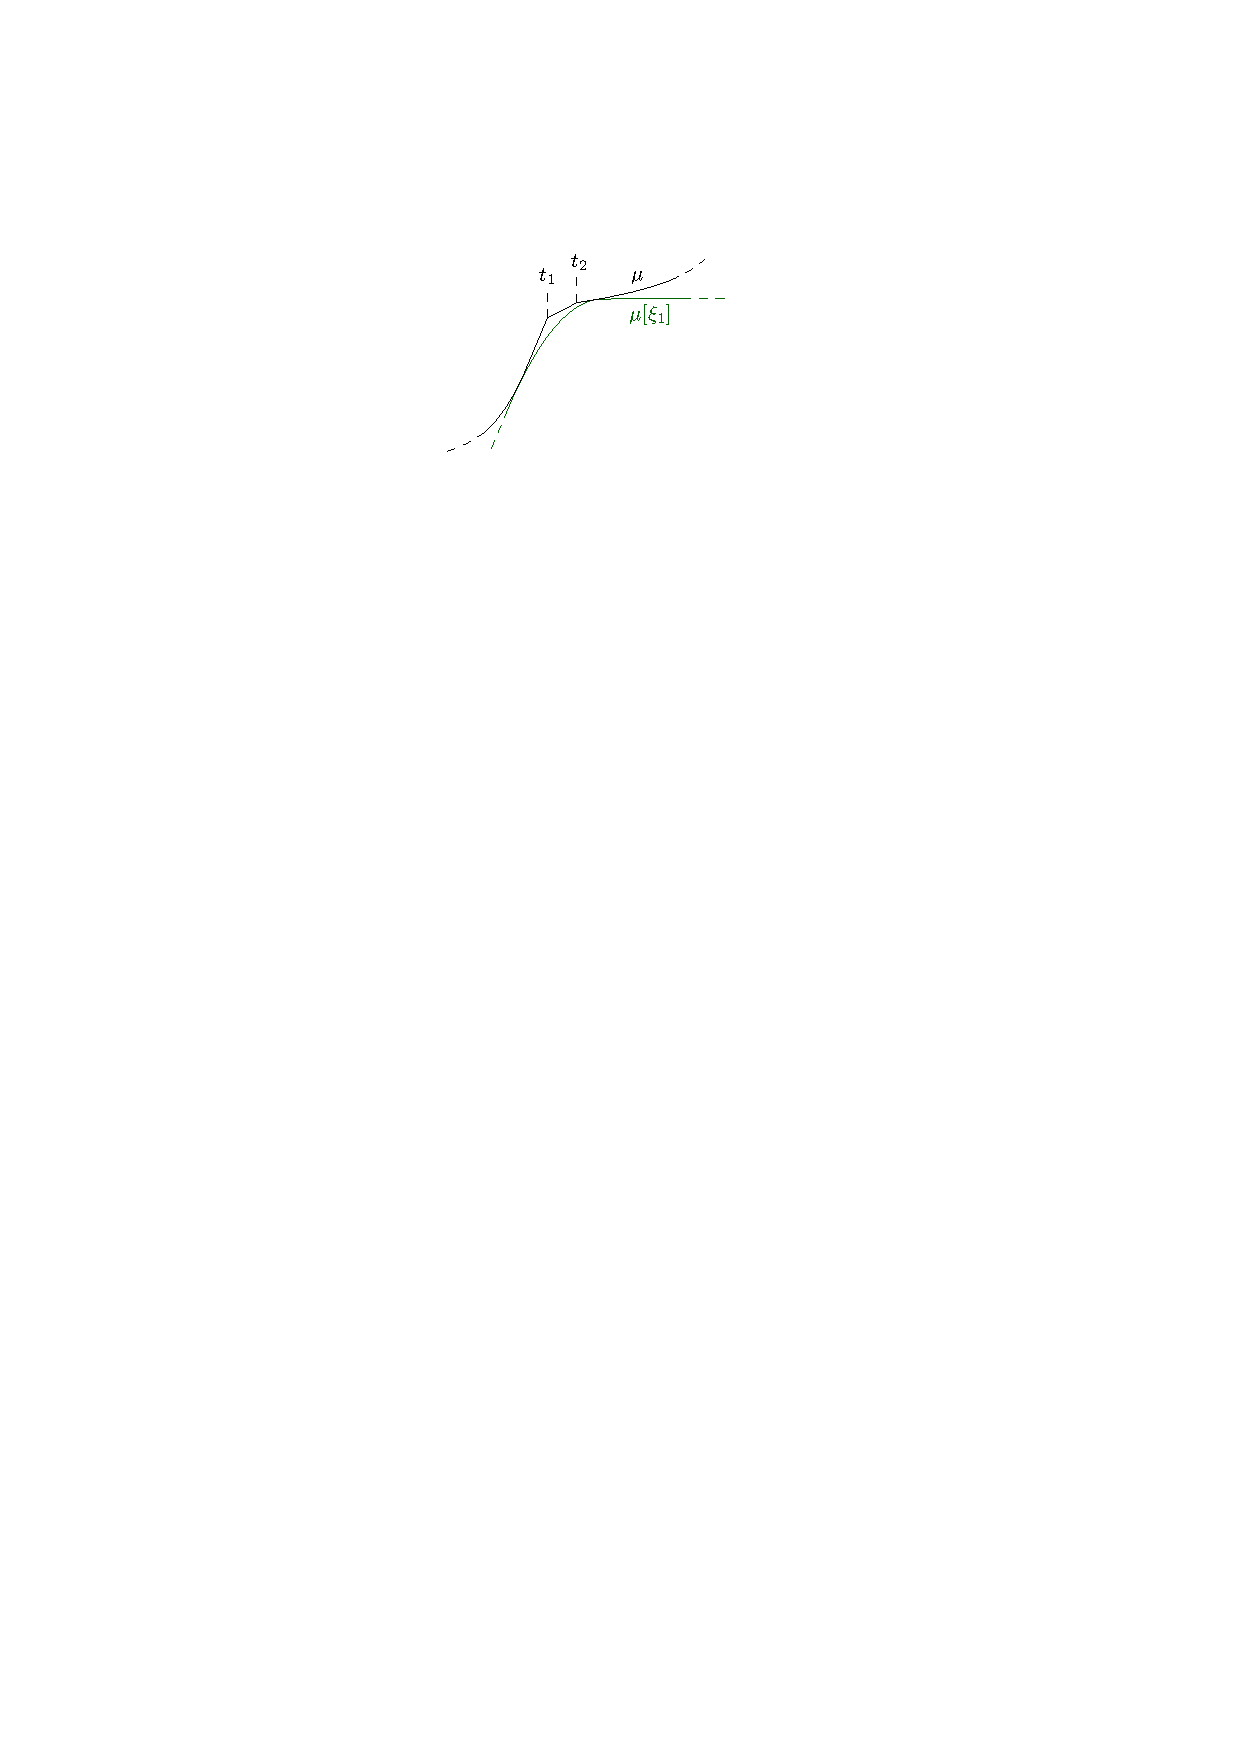
\includegraphics[scale=1.0]{figures/motion/multiple-discontinuities}
  \caption{Part of a piecewise trajectory $\mu$ on which a single connecting
    deceleration covers the two discontinuities at $t_{1}$ and $t_{2}$ at
    once.}%
  \label{fig:multiple-discontinuities}
\end{figure}

\paragraph{Proof of Theorem~\ref{thm:single-vehicle}.}
Let us now return to the minimum boundary $\gamma$ defined
in~\eqref{eq:min-boundary}.
%
From Figure~\ref{fig:necessary-conditions} and the conditions of
Theorem~\ref{thm:single-vehicle}, it is clear that $\gamma$ must satisfy
$\gamma(a) = A$, $\gamma(b) = B$ and \comment{I think this could be made more
  rigorous, but I think this is clear enough from the figure.}
$\dot{\gamma}(a) = \dot{\gamma}(b) = 1$, so whenever we have
$\gamma \in \mathcal{D}[a, b]$, i.e., $\gamma$ does not contain discontinuities,
we automatically have $\gamma \in D_{2}[a,b]$ so that $\gamma$ itself is already
a feasible solution.
%
\note{Explain why Assumption~\ref{assump:smoothing} holds.}
%
Otherwise, we perform the smoothing procedure presented above to obtain the
smoothed trajectory $\gamma^{*} \in \mathcal{D}[a,b]$.
%
This completes the proof of Theorem~\ref{thm:single-vehicle}.

\subsection{Upper boundary solution}\label{sec:upper-bound-property}

As a byproduct of the above analysis, the next lemma shows that the solution
$\gamma^{*}$ is also an upper boundary for any other feasible trajectory.

\begin{lemma}\label{lemma:upperbound}
  Let $\mu \in \mathcal{P}[a,b]$ be a piecewise trajectory and let
  $\mu^{*} \in \mathcal{D}[a,b]$ denote the result after smoothing. All
  trajectories $x \in \mathcal{D}[a, b]$ that are such that
  $x \preceq \mu$, must satisfy $x \preceq \mu^{*}$.
  \comment{Is this argument clear enough?}
\end{lemma}
\begin{proof}
  Consider some interval $(\xi, \tau)$ where we introduced some connecting
  deceleration boundary. Suppose there exists some $t_{d} \in (\xi, \tau)$ such that
  $x(t_{d}) > \mu(t_{d})$. Because $x(\xi) \leq \mu(\xi)$, this means that $x$ must
  intersect $\mu$ at least once in $\halfopen{\xi}{t_{d}}$, so let
  $t_{c} := \sup \, \{ t \in \halfopen{\xi}{t_{d}} : x(t) = \mu(t) \}$ be the latest
  time of intersection such that $x(t) \geq \mu(t)$ for all $t \in [t_{c}, t_{d}]$.
  There must be some $t_{v} \in [t_{c}, t_{d}]$ such that $\dot{x}(t_{v}) > \dot{\mu}(t_{v})$,
  otherwise
  \begin{align*}
    x(t_{d}) = x(t_{c}) + \int_{t_{c}}^{t_{d}} \dot{x}(t) \diff t \leq \mu(t_{c}) + \int_{t_{c}}^{t_{d}} \dot{\mu}(t) \diff t = \mu(d_{t}) ,
  \end{align*}
  which contradicts our choice of $t_{d}$. Hence, for every
  $t \in [t_{v}, \tau]$, we have
  \begin{align*}
    \dot{x}(t) \geq \dot{x}(t_{v}) - \omega (t - t_{v}) > \dot{\mu}(t_{v}) - \omega(t - t_{v}) = \dot{\mu}(t) .
  \end{align*}
  It follows that $x(\tau) > \mu(\tau)$, which contradicts the assumption
  $x \preceq \mu$.
\end{proof}

\begin{remark}
  The above upper boundary property has the following interesting consequence if
  we extend the single vehicle problem to an optimal control problem by
  considering maximizing the haste criterion $J(x)$ defined
  in~\eqref{eq:haste-objective} as optimization objective.
  %
  In particular, observe that it follows from the above lemma that any other
  $x \in D_{2}[a,b]$ satisfying $x \preceq u$ must also satisfy
  \begin{align}
    \int_{a}^{b} x(t) \diff t \leq \int_{a}^{b} \gamma^{*}(t) \diff t
  \end{align}
  Consequently, $x = \gamma^{*}$ is an optimal solution to the single vehicle
  optimal control problem
  \begin{align}
    \max_{x \in D_{2}[a,b]} J(x) \; \text{ such that } \; x \preceq u .
  \end{align}

\end{remark}


\section{Lane planning feasibility}\label{sec:lane-problem-feasibility}

We will now return to the feasibility of the lane planning problem and show how
it decomposes in terms of a sequence of single vehicle feasibility problems.
%
Let us first restate the conditions for feasible solutions of the lane planning
problem.
%
Recall that we are given schedule times $a = (a_{1}, a_{2}, \dots, a_{N})$ and
$b = (b_{1}, b_{2}, \dots, b_{N})$, which are assumed to be ordered as
$a_{1} \leq \dots \leq a_{N}$ and
$b_{1} \leq \dots \leq b_{N}$.
%
For brevity, we will write $x \in D_{2}^{N}[a, b]$ to denote the vector
$x = (x_{1}, \dots, x_{N})$ of $N$ trajectories $x_{i} \in D_{2}[a_{i},b_{i}]$.
%
Assume the system parameters $(\omega, \bar{\omega},A,B,L)$ to be fixed, then
the goal is to find a sequence of trajectories $x \in D_{2}^{N}[a,b]$ such that
\begin{subequations}
\begin{alignat}{2}
  &x_{i} \in D_2[a_{i},b_{i}] && \quad \text{ for each } i \in \{1, \dots, N\} , \\
  &x_{i} \preceq x_{i-1} - L && \quad \text{ for each } i \in \{2, \dots, N\} . \label{eq:follow-constraint}
\end{alignat}
\end{subequations}

%
The general idea is to repeat the construction of the previous section for each
vehicle to obtain a solution $x_{i}$, while using each constructed trajectory as
the boudary $u = x_{i}$ for the next problem of finding $x_{i+1} \preceq u$.
%
We will show that feasibility is equivalent to having the schedule times $a_{i}$
and $b_{i}$ satisfy a certain system of inequalities.
%
We will need the following technical assumption regarding the minimum length of
the lane, which is very reasonable to assume in practice.

\begin{assump}\label{assump:L-bound}
  Assume that vehicle lengths are limited by $L < B - A$.
\end{assump}

\begin{figure}
  \centering
  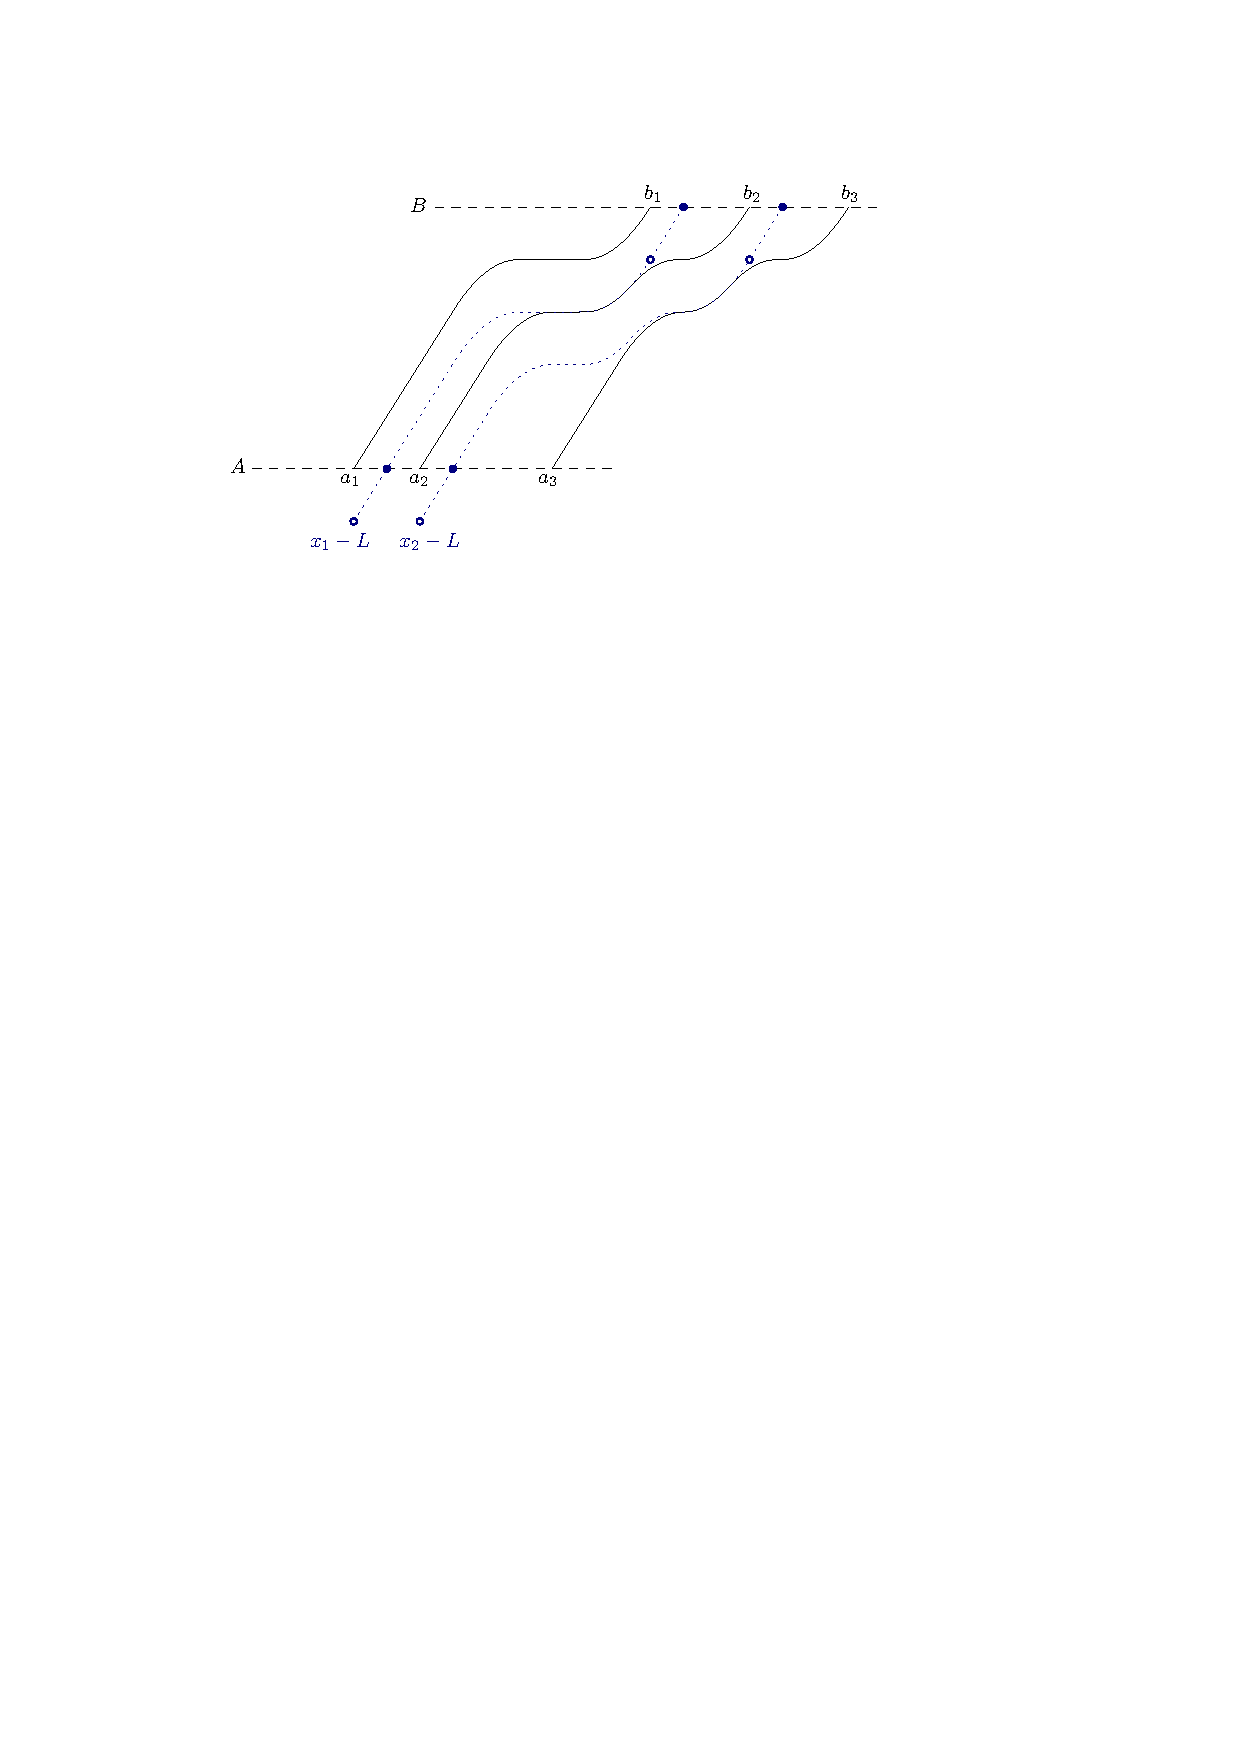
\includegraphics[scale=1.0]{figures/motion/solution}
  \caption{Optimal trajectories $x_{i}$ for three vehicles. The dotted blue
    trajectories between the little open circles illustrates the safe following
    constraints~\eqref{eq:follow-constraint}. The dotted blue trajectories between
    the solid dots are the following boundaries
    $\bar{x}_{2} \in \bar{D}[\bar{a}_{2}, \bar{b}_{2}]$ and
    $\bar{x}_{3} \in \bar{D}[\bar{a}_{3}, \bar{b}_{3}]$.}%
  \label{fig:solution}
\end{figure}

Now consider the safe following constraints~\eqref{eq:follow-constraint}.
%
We show how transform these into equivalent upper boundaries
$\bar{x}_{i} \in \bar{D}_{1}[\bar{a}_{i}, \bar{b}_{i}]$ for each
$i \in \{2, \dots, N\}$, such we can apply Theorem~\ref{thm:single-vehicle}.
%
It becomes clear from Figure~\ref{fig:solution} that
inequality~\eqref{eq:follow-constraint} only applies on some subinterval
$I_{i} \subset [a_{i-1}, b_{i-1}]$.
%
However, as the figure suggests, we can easily truncate and extend these
boundaries as necessary.
%
For some $y \in \mathcal{D}[\alpha, \beta]$, we define the inverse at some
position $p$ in its range to be
\begin{align}
  y^{-1}(p) = \inf \{ t \in [\alpha, \beta] : y(t) = p\} .
\end{align}
%
Given some trajectory $u \in D_{1}[c,d]$, we define its \emph{downshift}
%
\begin{align}
  \bar{u}(t) =
  \begin{cases}
    u(t) - L &\text{ for } t \in [u^{-1}(A + L), d] , \\
    B - L + t - d &\text{ for } t \in [d, d + L] .
  \end{cases}
\end{align}
For ease of reference, we denote the endpoints of its domain as
$\bar{a} := u^{-1}(A+L)$ and $\bar{b} := d + L$.

\begin{lemma}[Boundary extension]\label{lemma:boundary-extension}
  Consider some trajectory $u \in \mathcal{D}[c,d]$ such that $u(d) \geq A$. If
  $x \in \mathcal{D}[a,b]$ is such that $x(a) = A$ and $x \preceq u$, then it
  satisfies $x \preceq (u(d) + t - d)|_{\halfopen{d}{\infty}}$, which may be
  interpreted as extending the upper boundary $u$ to the right at full speed.
\end{lemma}
\begin{proof}
  If $b < d$, then $x \preceq (\cdot)|_{\halfopen{d}{\infty}}$ is always void and
  the statement is trivially true. Assume $b \geq d$ and consider an arbitrary
  $t \geq d$.
  %
  Suppose $a \leq d$, then we have $x(t) \leq x(d) + t - d \leq u(d) + t - d$.
  Suppose $a > d$, then we have $x(t) \leq x(a) + t - a = A + t - a \leq u(d) + t - d$.
\end{proof}
\begin{lemma}[Downshift boundary equivalence]\label{lemma:downshift}
  For each $u \in D_{2}[c,d]$, the downshift trajectory satisfies
  $\bar{u} \in D_{1}[\bar{a},\bar{b}]$.
  %
  \comment{Why do we assume $a \geq c$ and $b \geq d$ in the downshift lemma?
    Because we assume $a_{1} \leq a_{2} \leq \dots \leq a_{N}$ and similarly for
    $b_{i}$.}
  %
  For each $x \in D[a, b]$ such that $a \geq c$ and $b \geq d$, we have
  $x \preceq u - L$ if and only if $x \preceq \bar{u}$.
\end{lemma}
\begin{proof}
  The two cases in the definition of $\bar{u}$ coincide, so that
  $\bar{u} \in \mathcal{D}$. Furthermore, it is easily verified that
  $\bar{u}(\bar{a}) = A$ and $\bar{u}(\bar{b}) = B$, so the first claim
  follows.

  Suppose $x \preceq u - L$, and suppose there exists some
  $t \in [a,b] \cap [c,d]$. If $t \in [\bar{a}, d]$, then
  $x(t) \leq u(t) - L = \bar{u}(t)$ by definition. If $t \in [d, \bar{b}]$, then
  apply Lemma~\ref{lemma:boundary-extension} to $u - L$ (using
  Assumption~\ref{assump:L-bound} for $u(d) - L \geq A$) to obtain
  $x \leq (\tau \mapsto u(d) - L + \tau - d)|_{\halfopen{d}{\infty}} = (\tau \mapsto B - L + \tau - d)|_{\halfopen{d}{\infty}}$,
  so that $x(t) \leq B - L + t - d = \bar{u}(t)$.

  For the other direction, suppose $x \preceq \bar{u}$. First of all, since
  $u(c) = A$ and $u(\bar{a}) = A+L > A$ and $u$ is non-decreasing, we have
  $c < \bar{a}$.
  %
  Suppose $c \leq a < \bar{a}$, then since $b \geq d \geq \bar{a}$ and
  $\dot{x}(a) = 1$, we must have
  $x(\bar{a}) > x(a) = A = \bar{u}(\bar{a})$, contradicting the initial
  assumption.
  %
  Hence, $a \geq \bar{a}$, so any $t \in [a,b] \cap [c,d]$ satisfies
  $t \in [\bar{a}, d]$, but then $x(t) \leq \bar{u}(t) = u(t) - L$ by
  definition.
\end{proof}

%
The following lemma summarizes what we have established so far.

\begin{lemma}\label{lemma:summary}
  The following four statements are equivalent:

  \begin{enumerate}[leftmargin=3em]
    \item[(C0)] The lane planning problem is feasible.
    \item[(C1)] There exists $x \in D_{2}^{N}[a, b]$ such that $x_{i} \preceq x_{i-1} - L$ for all $i \in \{2, \dots, N\}$.
    \item[(C2)] There exists $x \in D_{2}^{N}[a, b]$ such that $x_{i} \preceq \bar{x}_{i-1}$ for all $i \in \{2, \dots, N\}$.

    \item[(C3)] There exists $x \in D_{2}^{N}[a, b]$ such that
          $b_{i} - a_{i} \geq B - A$ for all $i \in \{1, \dots, N\}$; and
    \TabPositions{2cm}
    \begin{enumerate}[label=(\roman*)\quad,leftmargin=3em,midpenalty=10]
      \item $b_{i} \geq \bar{b}_{i-1}$, \tab (exit order constraint)
      \item $a_{i} \geq \bar{a}_{i-1}$, \tab (entry order constraint)
      \item $\bar{x}_{i-1} \succeq \check{x}_{i}$, \tab (entry space constraint)
    \end{enumerate}
    for all $i \in \{2, \dots, N\}$.

  \end{enumerate}
\end{lemma}
\begin{proof}
  Of course, (C0) and (C1) are equivalent by definition of the lane planning
  problem. Note that equivalence of (C1) and (C2) is handled by Lemma~\ref{lemma:downshift}.
  %
  Equivalence of (C2) and (C3) follows from a straightforward application of
  Theorem~\ref{thm:single-vehicle} by setting $x=x_i$ and $u=\bar{x}_{i-1}$ for
  each $i \in \{2, \dots, N\}$.
\end{proof}

\paragraph{Simpler conditions.}
The goal of the remainder of this section is to get rid of the entry space
constraints and replace them with an inequality constraints in terms of schedule
times.
%
Moreover, we want to get rid of the dependence of $\bar{a}_{i-1}$ on
$\bar{x}_{i-1}$, such that we obtain equivalent statements in $a_{i-1}$. Note
that the exit order constraint is already in the desired form, because we have
$\bar{b}_{i-1} = b_{i-1} + L$.
%
More specifically, we will thus show that the statements of
Lemma~\ref{lemma:summary} above are further equivalent to:
\begin{enumerate}[leftmargin=3em]
  \item[(C4)] We have $b_{i} - a_{i} \geq B-A$ for all $i \in \{1, \dots, N\}$; and
  \begin{enumerate}[leftmargin=4em,midpenalty=10]
    \item[(i*)\quad] $b_{i} \geq b_{i-1} + L$,
    \item[(ii*)\quad] $a_{i} \geq a_{i-1} + L$,
  \end{enumerate}
  \TabPositions{3cm}
  for all $i \in \{2, \dots, N\}$; and
  \begin{enumerate}[leftmargin=4em,midpenalty=10]
    \item[(c*)\quad] $a_{i} \geq \check{a}_i(a,b)$, \tab (entry time constraint)
  \end{enumerate}
  for all $i \in \{n, \dots, N \}$,
\end{enumerate}
for some $n \geq 2$ and where $\check{a}_{i}(a,b)$ denotes some expression in terms of
schedule times. Consequently, $\max\{a_{i-1} + L, \check{a}_{i}(a,b)\}$ can be
interpreted as the earliest possible time of arrival to the lane for vehicle
$i$.

\note{Before we are able to prove this equivalence, we will need some better
  understanding of the smoothing procedure, so we will derive explicit formulas
  for finding the touching times $\xi$ and $\tau$ to obtain optimal trajectories
  under the hast objective.}

\section{Optimal solution for haste objective}\label{sec:explicit-trajectories}

Due to the recursive nature of the problem, we will see that optimal
trajectories for the haste objective (minimizing $J_{\alpha,\beta}$ with
$\alpha=-1,\beta=0$) possess a particularly simple structure, which enables a
simple computation.

\begin{define}
  Let a trajectory $\gamma \in \mathcal{D}[a, b]$ be called \emph{alternating} if for all
  $t \in [a, b]$, we have
  \begin{align}
    \ddot{\gamma}(t) \in \{-\omega, 0, \bar{\omega}\} \quad \text{ and } \quad
    \ddot{\gamma}(t) = 0 \implies \dot{\gamma}(t) \in \{0, 1\}.
  \end{align}
\end{define}

We now argue that each vehicle's optimal trajectory $x_{i}$ is alternating.
First, consider $x_{1} = x^{*}(a_{1}, b_{1}, \varnothing)$, which is
constructed by joining $x^{1}[x_{1}]$ and $\hat{x}[x_{1}]$ together by smoothing. Observe that both boundaries are alternating by definition. Let
$\gamma_{1}(t) = \min\{x^{1}[x_{1}](t), \hat{x}[x_{1}](t) \}$ be the minimum boundary,
then it is clear that the smoothened $x_{1} = \gamma_{1}^{*}$ must also be
alternating, because we only added a part of deceleration at some interval
$[\xi, \tau]$, which clearly satisfies $\ddot{\gamma}_{1}^{*}(t) = -\omega$ for
$t \in [\xi,\tau]$.
%
Assume that $x_{i-1}$ is alternating, we can similarly argue that $x_{i}$ is
alternating. Again, let
$\gamma_{i}(t) = \min\{\bar{x}[x_{i-1}], \hat{x}[x_{i}](t), x^{1}[x_{i}](t)\}$ be the
minimum boundary. After adding the required decelerations for smoothing, it is
clear that $x_{i} = \gamma^{*}_{i}$ must also be alternating.

\begin{figure}
  \centering
  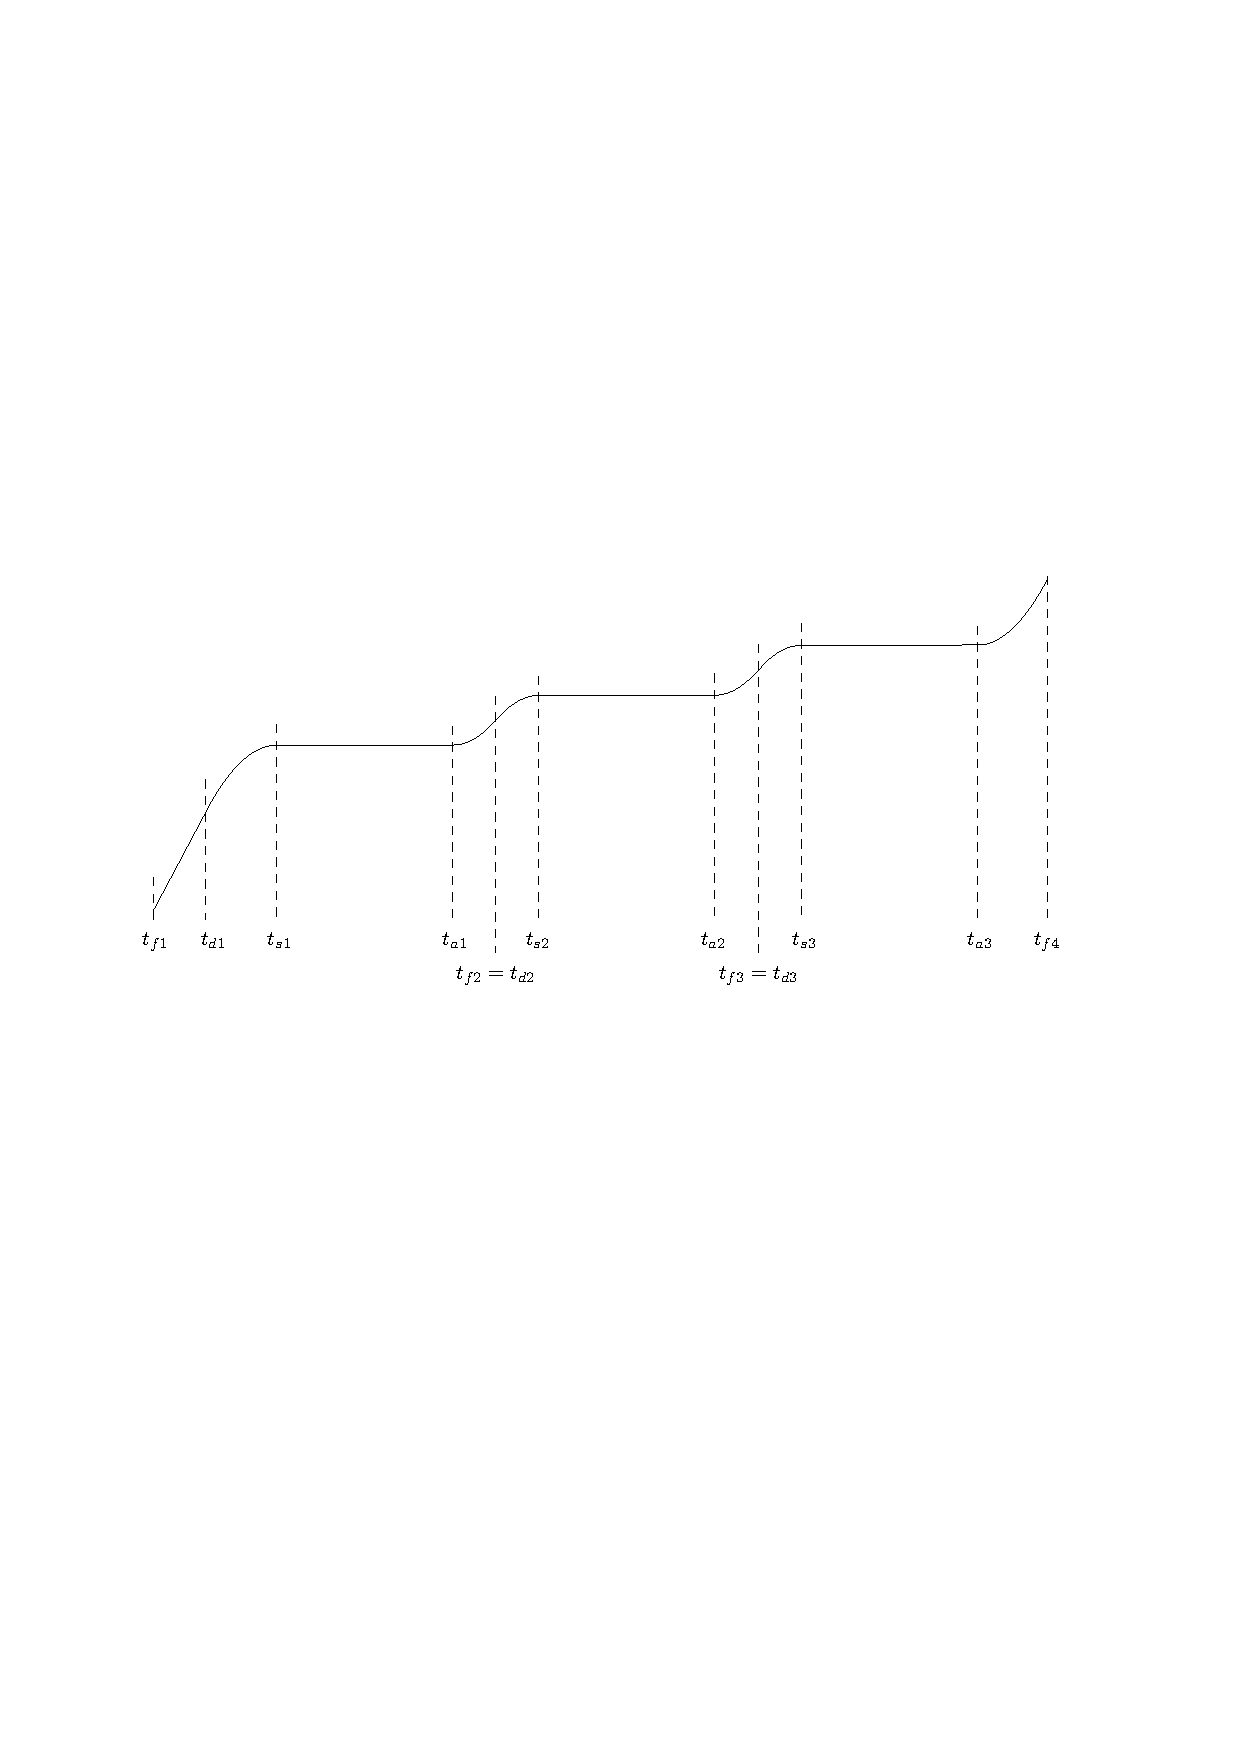
\includegraphics[scale=0.9]{figures/motion/tandem_trajectory}
  \caption{Example of an alternating vehicle trajectory with its defining time
    intervals. The particular shape of this trajectory is due to two leading
    vehicles, which causes the two start-stop \emph{bumps} around the times where these
    leading vehicles depart from the lane.}
  \label{fig:tandem_trajectory}
\end{figure}

Observe that an alternating trajectory $\gamma \in \mathcal{D}[a,b]$ can be described
as a sequence of four types of consecutive repeating phases, see
Figure~\ref{fig:tandem_trajectory} for an example.
%
In general, there exists a partition of $[a,b]$, denoted by
\begin{align*}
  a = t_{f1} \leq t_{d1} \leq t_{s1} \leq t_{a1} \leq t_{f2} \leq t_{d2} \leq t_{s2} \leq t_{a2} \leq \dots \leq t_{f,n+1} = b,
\end{align*}
such that we have the consecutive \emph{alternating intervals}
\begin{alignat*}{3}
  F_{i} &:= [t_{f,i}, t_{d,i}] \quad &\text{ (full speed), } \quad
  S_{i} &:= [t_{s,i}, t_{a,i}] \quad &\text{ (stopped), } \\
  D_{i} &:= [t_{d,i}, t_{s,i}] \quad &\text{ (deceleration), } \quad
  A_{i} &:= [t_{a,i}, t_{f,i+1}] \quad  &\text{ (acceleration), }
\end{alignat*}
%
such that on these intervals, $\gamma$ satisfies
%
\begin{alignat*}{4}
  &\dot{\gamma}(t) = 1 && \text{ for } t \in F_{i} , \quad \quad
  &&\dot{\gamma}(t) = 0 && \text{ for } t \in S_{i} ,\\
  &\ddot{\gamma}(t) = -\omega \quad && \text{ for } t \in D_{i} , \quad \quad
  &&\ddot{\gamma}(t) = \bar{\omega} \quad && \text{ for } t \in A_{i} .
\end{alignat*}

\paragraph{Partial trajectories.}
Next, we will define parameterized functions $x^{f}$, $x^{d}$, $x^{s}$, $x^{a}$
to describe alternating trajectory $\gamma$ on each of these alternating intervals.
%
Given some initial position $p \in [A,B]$, velocity $v \in [0, 1]$, start and end times $a$ and
$b$ such that $a \leq b$ and $v + \bar{\omega}(b - a) \leq 1$, we define the acceleration
trajectory $x^{a}[p, v, a, b] : [a, b] \rightarrow \mathbb{R}$ by setting
\begin{subequations}
\begin{align}
  x^{a}[p,v,a,b](\tau) &:= p + v(\tau - a) + \bar{\omega} (\tau-a)^{2} / 2 , \\
  \dot{x}^{a}[p,v,a,b](\tau) &:= v + \bar{\omega} (\tau - a) .
\end{align}
\end{subequations}
%
Similarly, for $p, v, a, b$ satisfying $a \leq b$ and $v - \omega(b-a) \geq 0$,
let the deceleration trajectory
$x^{d}[p, v, a, b] : [a, b] \rightarrow \mathbb{R}$ be defined as
\begin{subequations}
\begin{align}
  x^{d}[p,v,a,b](\tau) &:= p + v (\tau - a) - \omega (\tau - a)^{2} / 2 , \\
  \dot{x}^{d}[p,v,a,b](\tau) &:= v - \omega (\tau - a) .
\end{align}
\end{subequations}
%
One may notice that $x^{d}$ is essentially the same as the deceleration boundary
$x^{-}$, which we defined in Section~\ref{sec:deceleration-boundary}. However, note that the condition $v - \omega(b-a) \geq 0$ restricts the domain such that we do not need the clipping operation. Furthermore, the parameterization of $x^{d}$ will be more convenient in the next section.

We use the following notation for trajectories with constant minimum or maximum
speed. We write $x^{s}[p, a, b](\tau) \equiv p$, with domain $[a,b]$, to model a stopped
vehicle and let $x^{f}[p, a, b](\tau) = (p + \tau - a, 1)$ model a vehicle that drives
at full speed, also with domain $[a,b]$.


\subsection{Connecting partial trajectories}

It can be shown that the smoothing procedure introduces a part of deceleration
only between the four pairs of partial trajectories
\begin{align*}
    x^{a} \rightarrow x^{a} , \quad \quad
    x^{a} \rightarrow x^{s} , \quad \quad
    x^{f} \rightarrow x^{a} , \quad \quad
    x^{f} \rightarrow x^{s} .
\end{align*}
We will use these results to characterize optimal trajectories for our optimal
control problem.

\begin{lemma}[$x^{f} \rightarrow x^{s}$]
  Let $x^{f}[p, a, b]$ and $x^{s}[q, c, d]$ be two trajectories. Considering
  $\tau_{1}$ and $\tau_{2}$ as variables in the equation
  \begin{align*}
    x^{d}[x^{f}[p, a, b](\tau_{1}), \tau_{1}, \tau_{2}](\tau_{2}) = x^{s}[q, c, d](\tau_{2}) ,
  \end{align*}
  it has solution
  $\tau_{2} = q - p + a + 1/2\omega$ and $\tau_{1} = \tau_{2} - 1/\omega$, whenever
  $\tau_{1} \in [a, b]$ and $\tau_{2} \in [c, d]$.
\end{lemma}
\begin{proof}
  The expanded system of state equations is given by
  \begin{align*}
    \begin{cases}
      p + \tau_{1} - a + (\tau_{2} - \tau_{1}) - \omega(\tau_{2} - \tau_{1})^{2} / 2 = q , \\
      1 - \omega(\tau_{2} - \tau_{1}) = 0 .
    \end{cases}
  \end{align*}
  The second equation yields $\tau_{2} - \tau_{1} = 1/\omega$, which after
  substituting back in the first equation yields
  $p - a + \tau_{2} - 1/2\omega - q = 0$, from which the stated solution
  follows.
\end{proof}


\begin{figure}
\centering
\begin{minipage}{.45\textwidth}
  \centering
  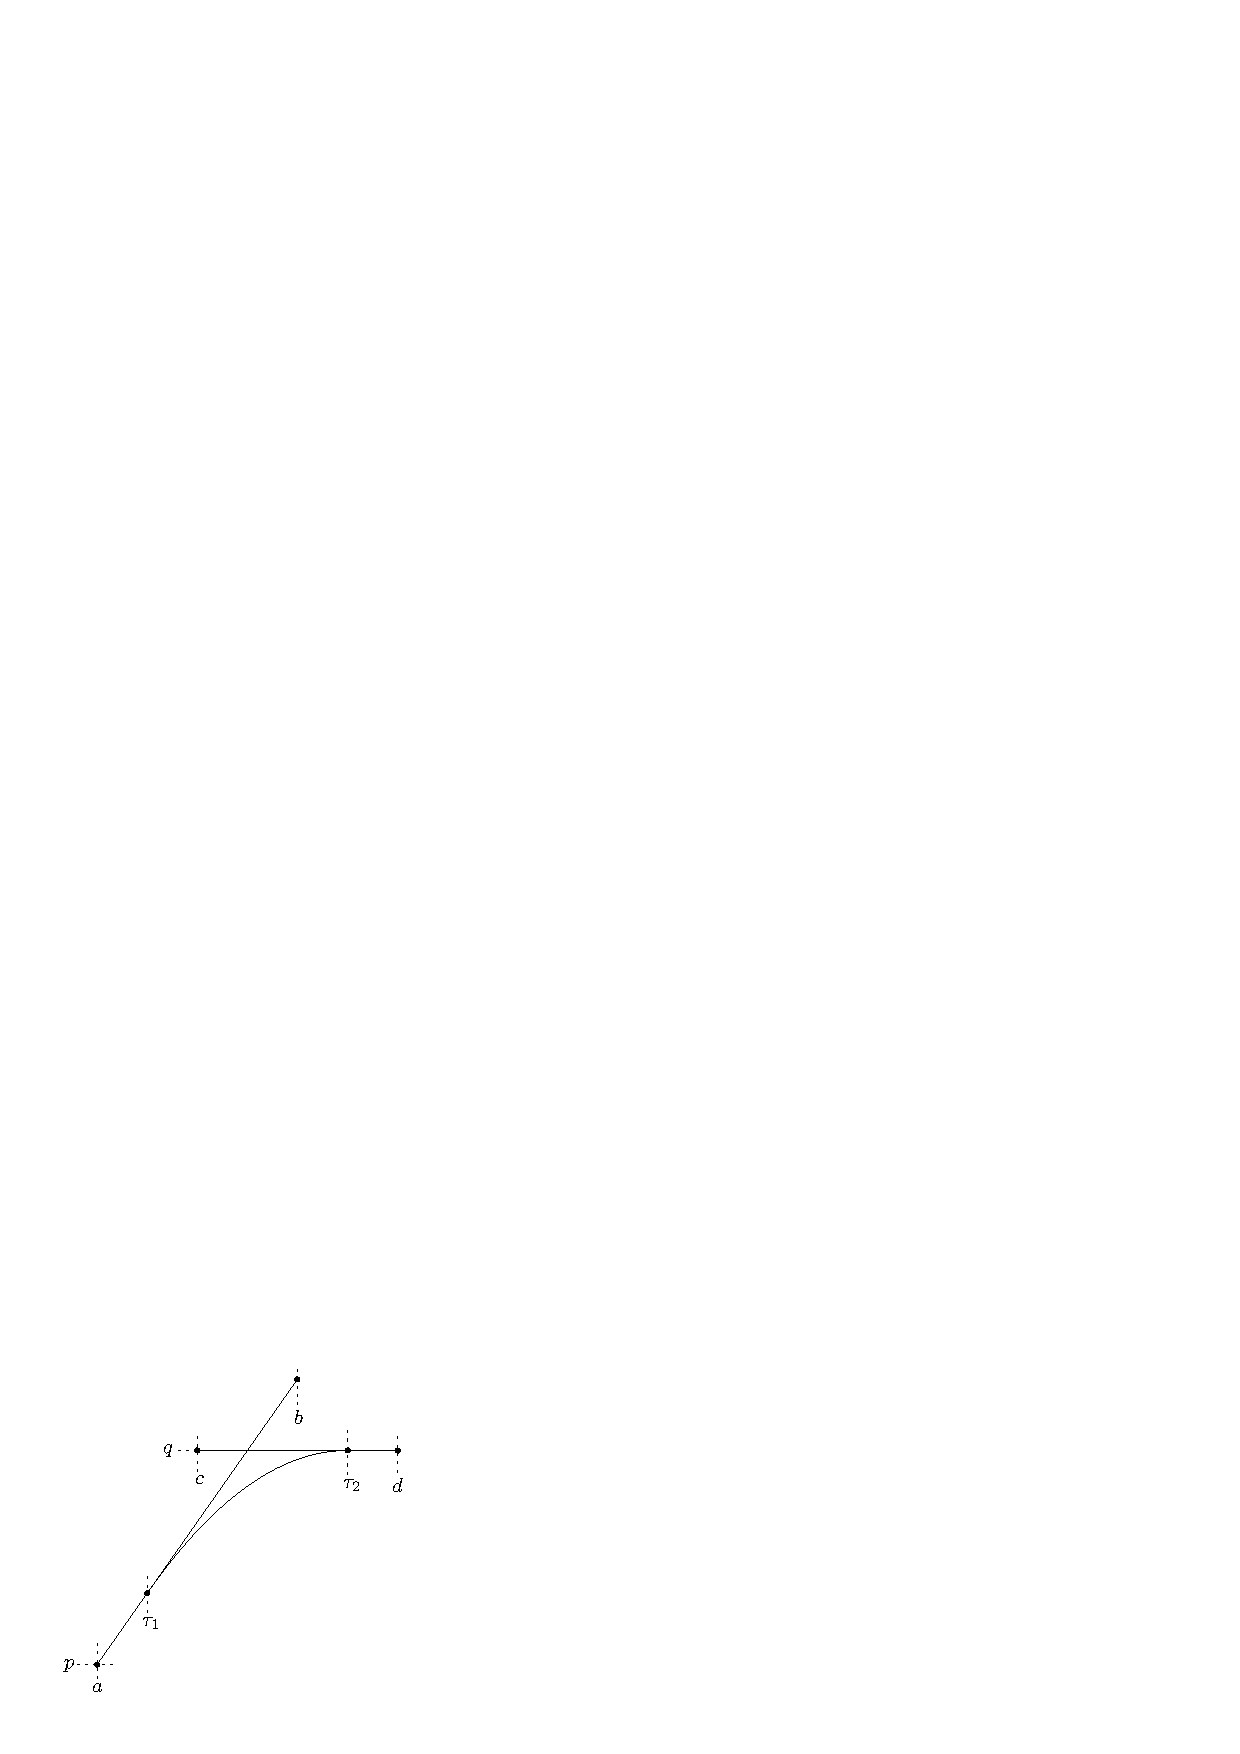
\includegraphics[width=0.9\linewidth]{figures/motion/lemma_full_still}
  \captionof{figure}{$x^{f} \rightarrow x^{s}$}
  \label{fig:full_still}
\end{minipage}%
\hspace{1.0em}
\begin{minipage}{.45\textwidth}
  \centering
  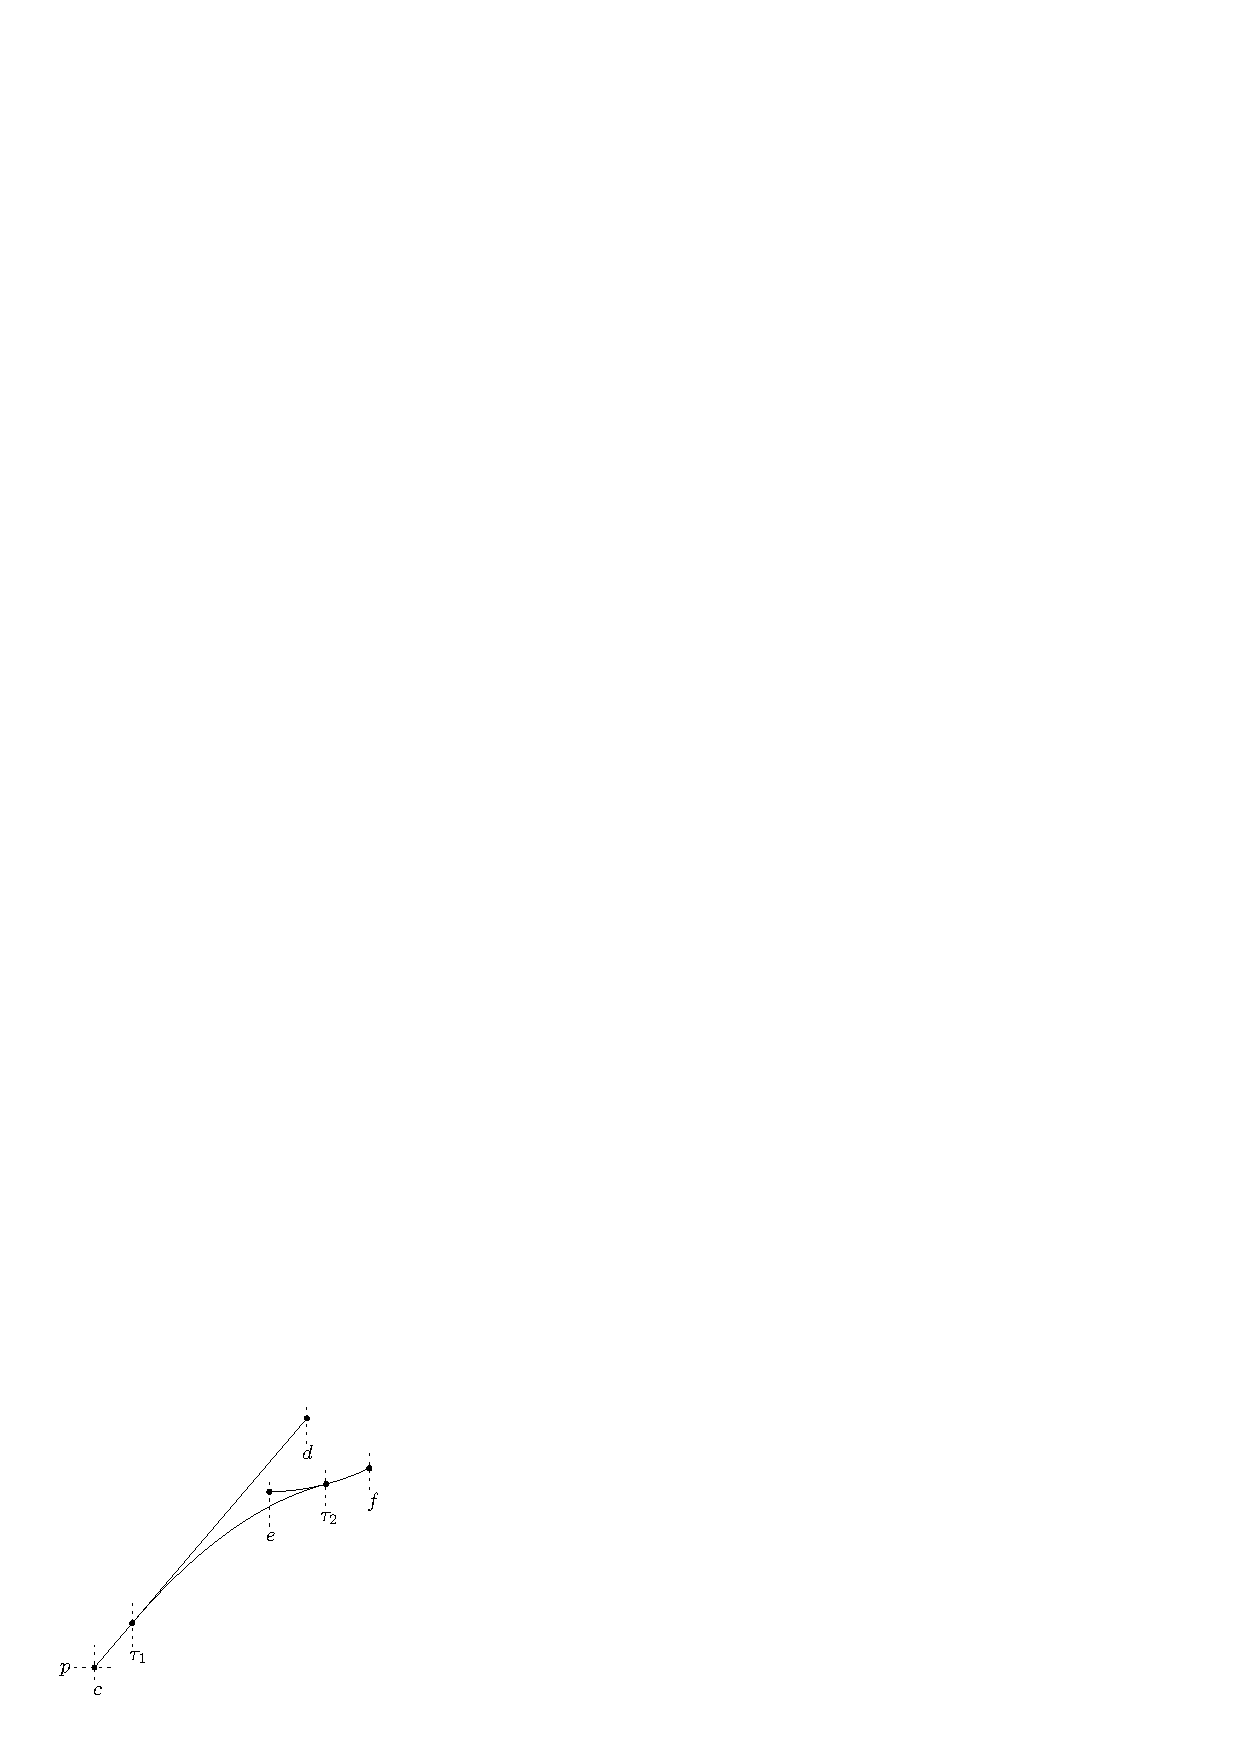
\includegraphics[width=0.9\linewidth]{figures/motion/lemma_full_acc}
  \captionof{figure}{$x^{f} \rightarrow x^{a}$}
  \label{fig:full_acc}
\end{minipage}
\end{figure}

To keep the expressions for the case of joining $x^{f} \rightarrow x^{a}$ a
little bit simpler, we first consider a full line joining to a acceleration
trajectory of full length $1/\omega$.

\begin{lemma}
  \label{lemma:line_acc}
  Consider some full acceleration trajectory $x^{a}[(p, 0), a, a+1/\omega]$ and the
  line through $(\lambda, 0)$ with slope 1. Whenever $\lambda$, which can be
  interpreted as a time epoch, satisfies $\lambda \in [a-p-1/2\omega, a-p+1/2\omega]$, then the equation
  \begin{align*}
    x^{+}[(p, 0), a, a+1/\omega](\tau) = x^{d}[(q, 1), q + \lambda, q + \lambda + 1/\omega](\tau) ,
  \end{align*}
  with $\tau$ and $q$ considered as variables, has a unique solution
  \begin{align*}
    \tau &= a + 1/\omega - \sqrt{\frac{a - p + 1/2\omega - \lambda}{\omega}} , \\
    q &= 2\tau - a - 1/\omega - \lambda ,
  \end{align*}
  so the joining deceleration is given by $x^{d}[(q,1), q + \lambda, \tau]$
\end{lemma}
\begin{proof}
  First of all, the expanded system of state equations is given by
  \begin{align*}
    \begin{cases}
    p + \omega (\tau - a)^{2}/2 = q + (\tau - q - \lambda) - \omega (\tau - q - \lambda)^{2}/2 , \\
    \omega(\tau - a) = 1 - \omega(\tau - q - \lambda) .
      \end{cases}
  \end{align*}
  We use the second equation to express $q$ in terms of $\tau$, which yields
  \begin{align*}
    q = 2\tau - 1/\omega -a - \lambda ,
  \end{align*}
  which we substitute in the first equation to derive the equation
  \begin{align*}
    \omega \tau^{2}  - 2 (1 + \omega a) \tau + \omega a^{2} + a + p + \lambda + 1/2\omega = 0 .
  \end{align*}
  This is a quadratic equation in $\tau$, with solutions
  \begin{align*}
    \tau = a + 1/\omega \pm \sqrt{\frac{a - p + 1/2\omega - \lambda}{\omega}} ,
  \end{align*}
  of which only the smallest one is valid, because $\tau \leq a + 1/\omega$.
  Furthermore, we see that $\tau$ is defined as a real number when
  \begin{align*}
    a - p + 1/2\omega - \lambda \geq 0 \iff \lambda \leq a - p + 1/2\omega .
  \end{align*}
  The other requirement is that $\tau \geq a$, which is equivalent to
  \begin{align*}
    1/\omega \geq \sqrt{\frac{a - p + 1/2\omega - \lambda}{\omega}} \iff
    % 1/\omega \geq a - p - \lambda + 1/2\omega \iff
    \lambda \geq a - p - 1/2\omega .
  \end{align*}
\end{proof}

\begin{lemma}[$x^{f} \rightarrow x^{a}$]
Consider partial trajectories $x^{f}[p, c, d]$ and $x^{a}[x, e, f]$.
\end{lemma}
\begin{proof}
  First of all, observe that $x^{f}[p, c, d]$ lies on the line with slope 1
  through $(\lambda, 0) := (c - p, 0)$ and $x^{a}[x, e, f]$ lies on the full
  acceleration curve
  $x^{a}[(x_{1} - x_{2}^{2}/(2\omega) , 0), e - x_{2}/\omega, e - x_{2}/\omega + 1/\omega]$, see
  Figure~\ref{fig:full_acc}.
  %
  Now apply Lemma~\ref{lemma:line_acc} to $p = x_{1} - x_{2}^{2}/(2\omega)$,
  $a = e - x_{2}/\omega$ and $\lambda = c - p$ yields some solutions $\tau$ and $q$.
  %
  Let $\tau_{2} := \tau$ and let $\tau_{1}$ denote the time where the line and
  $x^{a}$ join, given by $\tau_{1} = \lambda + q$. Now we simply check whether this
  solution is also feasible for the smaller trajectories. We must have
  $\tau_{1} \in [c, d]$ and $\tau_{2} \in [e, f]$.
\end{proof}


\begin{lemma}
  \label{lemma:acc_hline}
  Consider the acceleration trajectory $x^{a}[(p, 0), a, b]$ and the horizontal
  line through $(0, q)$. Let $\tau_{1} = a + \sqrt{(q-p)/\omega}$ and
  $\tau_{2} = a + 2\sqrt{(q-p)/\omega}$. If $\tau_{1}$ satisfies
  $\tau_{1} \in [a, b]$, then both trajectories are joined by deceleration
  trajectory $x^{d}[x^{a}[(p, 0), a, b](\tau_{1}), \tau_{1}, \tau_{2}]$
\end{lemma}
\begin{proof}
  Consider the following equation
  \begin{align*}
    x^{d}[x^{a}[(p, 0),a,b](\tau_{1}), \tau_{1}, \tau_{2}](\tau_{2}) = (q, 0) .
  \end{align*}
  %
  The expanded system of state equations is given by
  \begin{align*}
    \begin{cases}
      p + \omega (\tau_{1} - a)^{2}/2 + (\omega(\tau_{1} - a)) (\tau_{2} - \tau_{1}) - \omega(\tau_{2} - \tau_{1})^{2}/2 = q , \\
      \omega(\tau_{1} - a) - \omega(\tau_{2} - \tau_{1}) = 0 .
    \end{cases}
  \end{align*}
  From the second equation, we derive $\tau_{1} - a = \tau_{2} - \tau_{1}$.
  Plugging this back in the first equation yields the quadratic equation
  $p + \omega(\tau_{1} - a)^{2} = q$ with solutions
  $\tau_{1} = a \pm \sqrt{(q-p)/\omega}$, of which only the larger one is valid.
  Finally, the second equation gives $\tau_{2} = 2\tau_{1} - a$.
\end{proof}

\begin{lemma}[$x^{a} \rightarrow x^{s}$]
  Consider partial trajectories $x^{a}[x, c, d]$ and $x^{s}[q, e, f]$.
\end{lemma}
\begin{proof}
  Observe that $x^{a}[x, c, d]$ lies on the full acceleration curve
  $x^{a}[(x_{1} - x_{2}^{2}/(2\omega), 0), c - x_{2}/\omega, c - x_{2}/\omega + 1/\omega]$.
  Hence, we can apply Lemma~\ref{lemma:acc_hline} with
  $p=x_{1} - x_{2}^{2}/(2 \omega)$, $a = c - x_{2}/\omega$, which yields some
  solutions $\tau_{1}$ and $\tau_{2}$, which are feasible solutions if
  $\tau_{1} \in [c, d]$ and $\tau_{2} \in [e, f]$.
\end{proof}

\begin{lemma}
  Consider full acceleration trajectories $x^{a}[(p, 0), a, b]$ and
  $x^{a}[(q, 0), c, d]$.
\end{lemma}
\begin{proof}
  Consider the equation
  \begin{align*}
    x^{d}[x^{a}[(p, 0), a, b](\tau_{1}), \tau_{1}, \tau_{2}](\tau_{2}) = x^{a}[(q, 0), c, d](\tau_{2}) ,
  \end{align*}
  expanded to the system of equations
  \begin{align*}
    \begin{cases}
      p + \omega(\tau_{1} - a)^{2}/2 + \omega(\tau_{1} - a)(\tau_{2} - \tau_{1}) - \omega(\tau_{2} - \tau_{1})^{2}/2 = q + \omega(\tau_{2} - c)^{2}/2 , \\
      \omega(\tau_{1} - a) + \omega(\tau_{2} - \tau_{1}) = \omega(\tau_{2} - c) .
    \end{cases}
  \end{align*}
\end{proof}

\begin{lemma}[$x^{a} \rightarrow x^{a}$]
  Consider partial trajectories $x^{a}[x, a, b]$ and $x^{a}[y, c, d]$.
\end{lemma}
\begin{proof}

\end{proof}

\subsection{Algorithm}

Put everything together into pseudocode.

\begin{algorithm}
  \caption{Computing connecting deceleration for alternating trajectories.}
    \label{alg:connecting}
    \begin{algorithmic}
      \State Let $i$ such that $I_{i}$ is the latest such that $t_{1} < I_{i}$.
      \State Let $j$ such that $I_{j}$ is the earliest such that $t_{1} > I_{j}$.
    \end{algorithmic}
\end{algorithm}


\section{Feasibility characterization}

\paragraph{Waiting positions.}
Waiting capacity is given by
\begin{align}
  C = \left\lfloor \frac{B-A-1/(2\bar{\omega}) -1/(2\omega)}{L} \right\rfloor + 1 ,
\end{align}
where the brackets indicate the floor function.


\begin{figure}
  \centering
  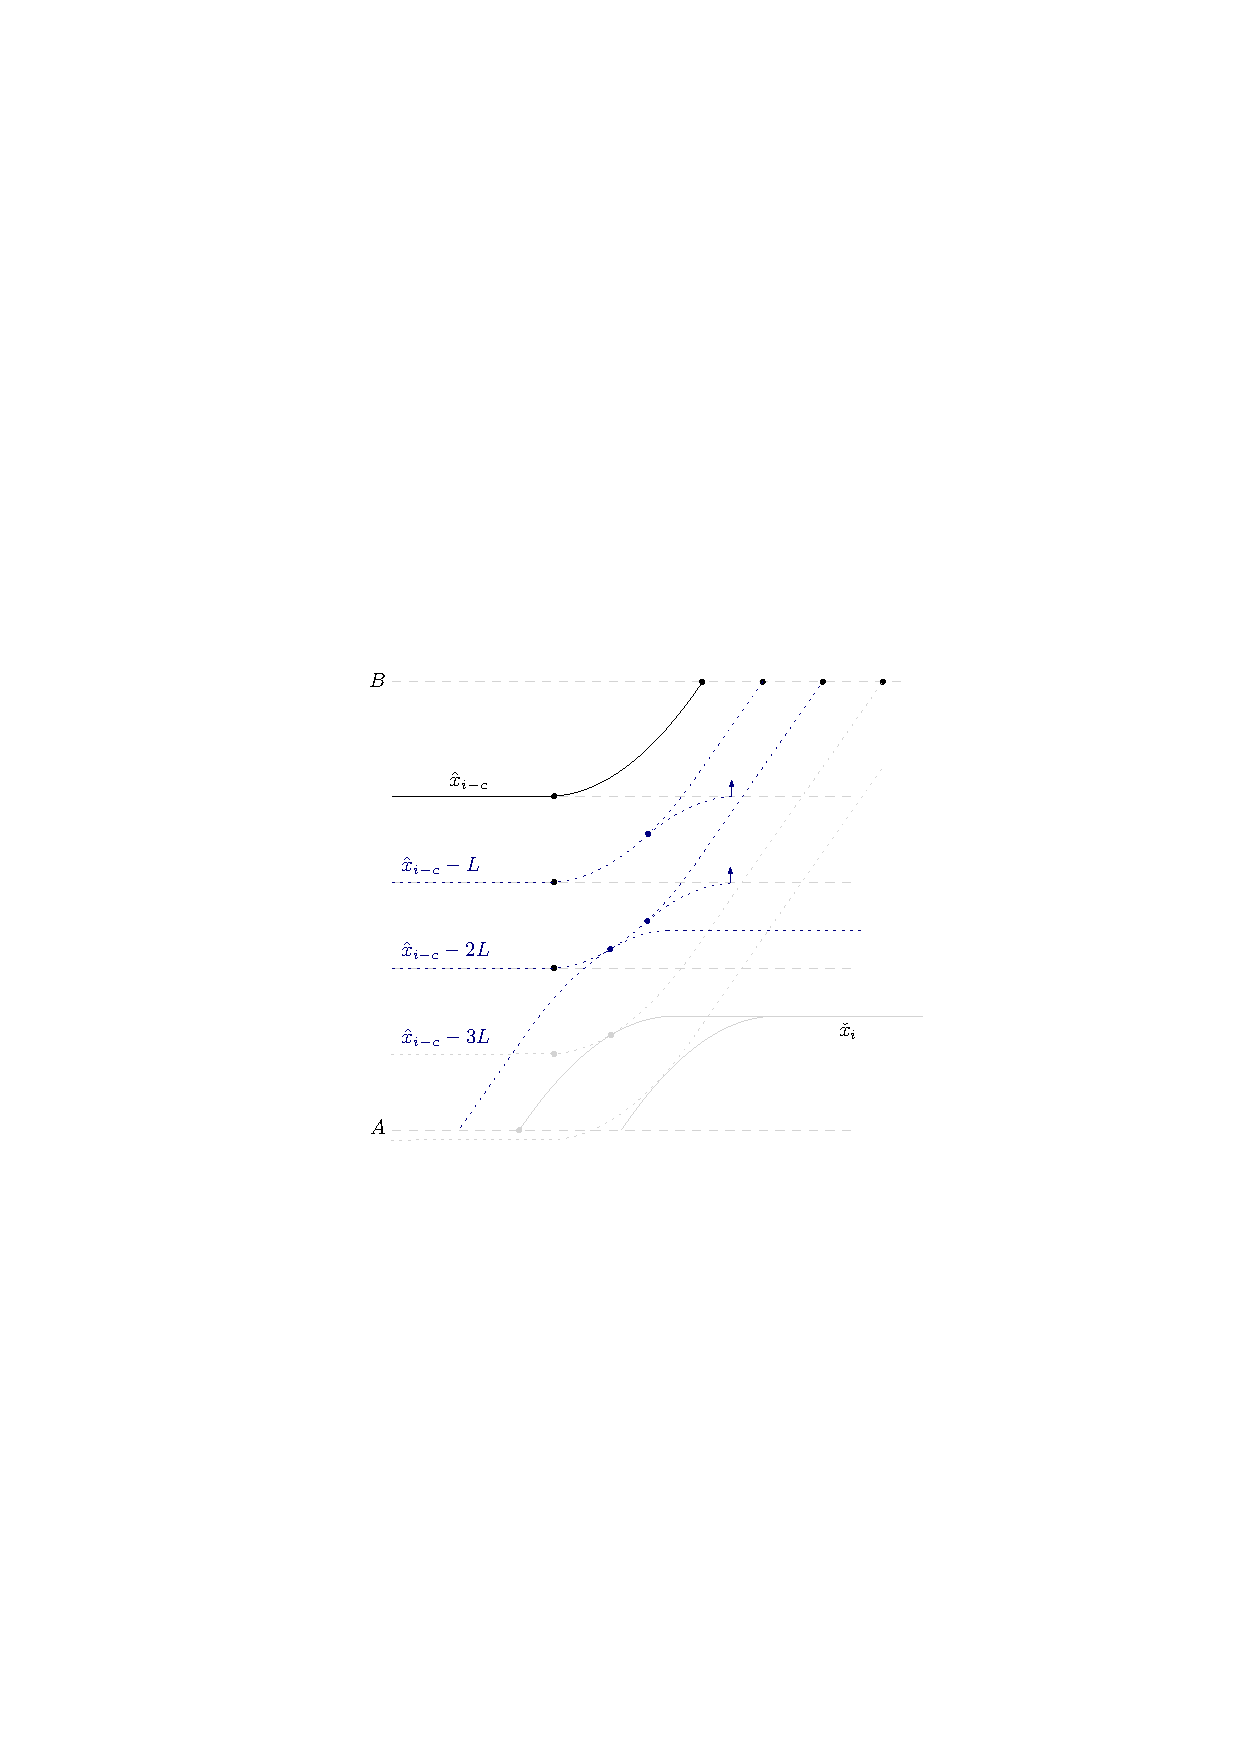
\includegraphics[scale=1]{figures/motion/earliest-arrival}
 \caption{Earliest arrival due to entry order constraint and entry space constraint.}%
\end{figure}



\section{Notes and references}

The analysis of feasibility conditions in this chapter is very much related to
the proof of the safety guarantee in~\cite{miculescuPollingsystemsbasedAutonomousVehicle2016}, see their Lemma IV.4 with
relatively long proof in appendix.
%
They study the online situation, in which new vehicles arrive to the system at
later times, for which they show that the rescheduling policy is safe, in the
sense that there are still feasible and collision-free trajectories for the
vehicles whose crossing times got updated.
%
We do not study such an online setting, but we take into account the fact that
lanes are of finite length.

We emphasize that the assumption $\dot{x}(a) = \dot{x}(b) = 1$ was mainly made
for convenience.
%
There are different ways of relaxing the state constraints on the speed that
could be studied.
%
The interesting question is whether feasibility can still be easily characterized.
%
Instead of fixing the speed to be maximal at entry and exit, we could require,
for example, that the speed is bounded from below, i.e., $\eta \leq \dot{x}(a) \leq 1$
and $\eta \leq \dot{x}(b) \leq 1$, for some $\eta > 0$.
%
The motivation for studying this relaxation is that this might lead to more
energy efficient trajectories, whenever full speed crossing is not strictly
necessary.


\addtocontents{toc}{\protect\renewcommand\cftbeforechapskip{2.5em}}
\chapter{Conclusion and discussion}\label{chap:conclusion}
\addtocontents{toc}{\protect\renewcommand\cftbeforechapskip{1em}}

\begin{outline}
  \1 new insights from current work
  \1 possible impact of this work
  \1 limitations of current work
  \1 recommendations on further work
\end{outline}

\paragraph{Contributions.}
\begin{outline}

  \1 Definition an analysis of single intersection coordination as offline
  optimization problem.
  \2 Expose computational challenge by formulating a bilevel decomposition.
  \2 Reduction to scheduling problem when additional assumptions are made.
  \2 Further reduction to sequencing problem (Section~\ref{sec:sequence-representation}).

  \1 Illustrate the ML for CO methodology for a relatively simple sequencing
  problem, arising from the single intersection coordination problem for
  autonomous vehicles.

  \1 Explicit trajectory calculation
  \2 For haste objective
  \2 For general arrival/crossing times (cf. Timmerman, Joshi)
\end{outline}


\paragraph{Beyond proper decomposition.}

We would like to drop the assumption of full speed crossing and allow more
general performance measures.
%
In this general setting, the problem does not properly decompose, so the upper-
and lower-level problems must be considered simultaneously.
%
We recognize that feasibility of the lower-level problem is a complicating
factor, because it puts difficult-to-formalize constraints on the upper-level
combinatorial problem.
%
We wonder whether it is possible to use ML to approximate these constraints
somehow. In other words, can we approximate the space of feasible solutions
somehow, with some guarantees?
%
The other complicating factor is the fact that the optimization objective is now a non-trivial function of the upper-level decisions variables.
%
However, this is a very natural candidate for approximation, and something similar has already been done before \note{[retrieve this paper]}.


% the code around the bibliographp itself serves as
% a sort of anchor for adding a bookmark entry
\phantomsection
\begin{singlespacing}\raggedright
\bibliographystyle{unsrt}
\bibliography{references}\label{sec:references}
\end{singlespacing}
% add entry to documents table of contents
\addcontentsline{toc}{chapter}{Bibliography}


\appendix

% add '.' after appendices in pdf bookmark, to avoid misreading 'A' as the first
% word of a sentence
% TODO: only do this at the top level
\let\origthechapter\thechapter
\makeatletter
\xpatchcmd{\addcontentsline}{%
\Hy@writebookmark{\csname the#2\endcsname}%
      {#3}%
      {\@currentHref}%
      {\Hy@toclevel}%
      {#1}%
}{%
\begingroup
\renewcommand{\thechapter}{\origthechapter.}
\Hy@writebookmark{\csname the#2\endcsname}%
{#3}%
{\@currentHref}%
{\Hy@toclevel}%
{#1}%
\endgroup
}{\typeout{Success}}{}
\makeatother

% % non-bold appendix entries
% \addtocontents{toc}{\protect
% \renewcommand{\protect\cftchapaftersnumb}{\normalfont}
% }
% % ...also non-bold page numbers
% \addtocontents{toc}{\protect
% \renewcommand{\protect\cftchappagefont}{\normalfont}
% }
% % decrease space between appendix entries
% \addtocontents{toc}{\protect
% \renewcommand{\protect\cftbeforechapskip}{\vskip0pt}
% }



\part*{Appendix}
\addcontentsline{toc}{part}{Appendix}

\chapter{Feasible configurations for single intersection model}\label{app:configuration-space}

\begin{figure}
  \centering
  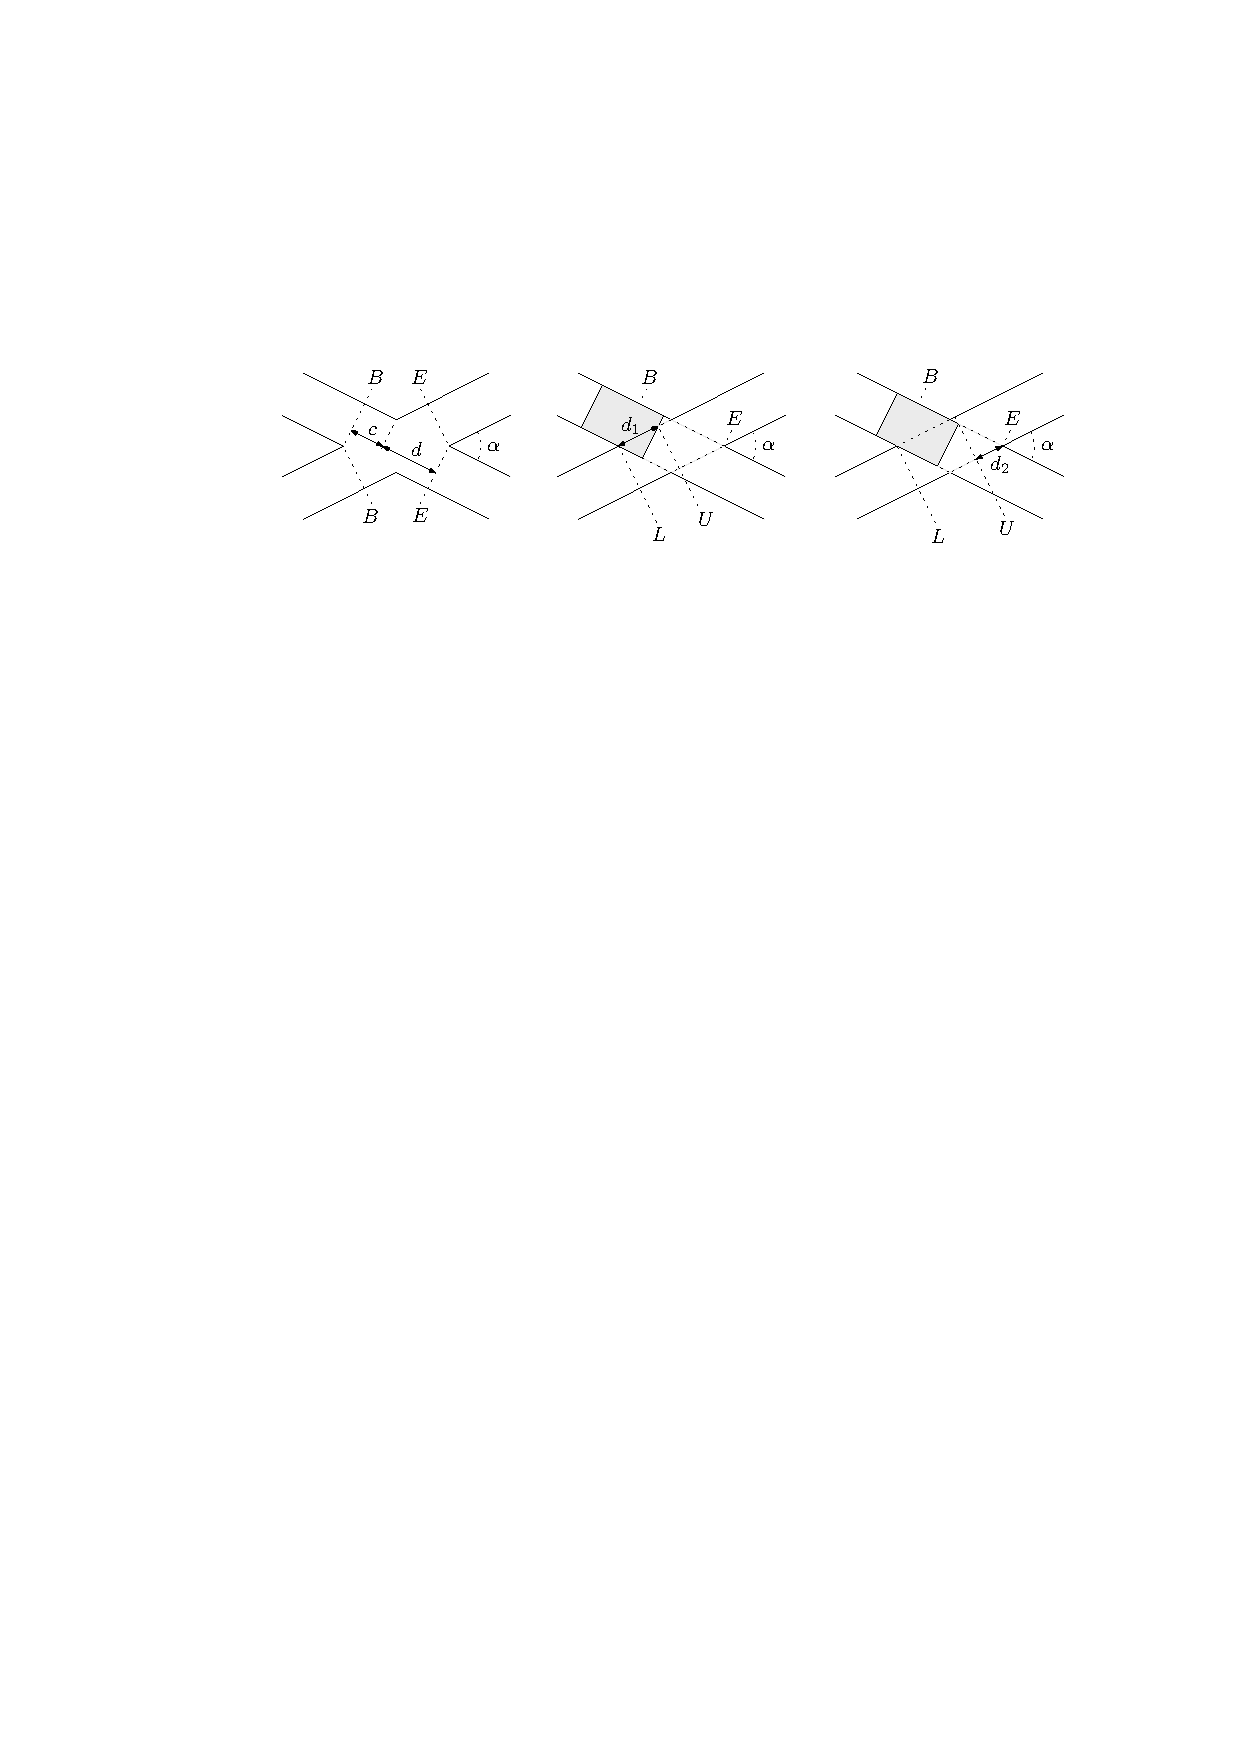
\includegraphics[scale=1]{figures/configuration-space}
  \caption{Sketches to derive the feasible configurations of two vehicles in the
    intersecting routes model. Using some elementary trigonometry, the distances
    in the first figure can be shown to be $c = W / \tan(\alpha)$ and
    $d = W / \sin(\alpha)$. Furthermore, observe that we have
    $(x_{i} - B) / d_{1} = \cos(\alpha)$ for
    $x_{i} \in \openhalf{B}{B + c}$, as shown in the middle figures and
    $d_{2}/(E - x_{i}) = \cos(\alpha)$ for $x_{i} \in \halfopen{B + c}{E}$,
    as shown in the right figure. These two types of distances can be used to
    derive the full characterization.}
  \label{fig:configuration-space}
\end{figure}

We present a way to derive the feasible configurations of the two routes that
intersect at some arbitrary angle, as shown in Figure~\ref{fig:intersection-non-axis-aligned}.
% general case
Assume that $\alpha < \pi / 2$ is the acute angle between the two intersections.
%
Furthermore, we consider uniform rectangular vehicle geometries with
$L_{i} \equiv L$ and $W_{i} \equiv W$, but the analysis is easily extended to
arbitrary dimensions.
%
We skip a thorough derivation of the following expressions, but we note that it
is based on the type of the distances illustrated in
Figure~\ref{fig:configuration-space}.
%
Roughly speaking, we encode the part of the intersection that vehicle $i$
occupies in terms of the other vehicle's $x_{j}$ coordinates, by defining the
following upper and lower limit positions
\begin{align}
  u(x_{i}) &:=
  \begin{cases}
    -\infty & \hspace{1.9em} \text{ if } x_{i} \leq B \text{ or } x_{i} - L \geq E , \\
    B + (x_{i} - E) / \cos(\alpha) & \hspace{1.9em} \text{ if } x_{i} \in \openhalf{E}{E + c\,} , \\
    E + (x_{i} - E) \cdot \cos(\alpha) & \hspace{1.9em} \text{ if } x_{i} \in \halfopen{E + c}{E} , \\
    E & \hspace{1.9em} \text{ if } x_{i} \geq E \text{ and } x_{i} - L < E ,
  \end{cases} \\
  l(x_{i}) &:=
  \begin{cases}
    B & \text{ if } x_{i} - L \leq E \text{ and } x_{i} > E , \\
    B + (x_{i} - L - E) / \cos(\alpha)     & \text{ if } x_{i} - L \in \openhalf{E}{E - c\,} , \\
    E + (x_{i} - L - E) \cdot \cos(\alpha) & \text{ if } x_{i} - L \in \halfopen{E - c}{E} , \\
    \infty & \text{ if } x_{i} - L \geq E \text{ or } x_{i} \leq E .
  \end{cases}
\end{align}
With these definitions, in order for the intersection to be free for vehicle
$j$, position $x_{i}$ must satisfy either $x_{i} < l(x_{j})$ or
$x_{i} - L > u(x_{j})$ and $x_{j}$ must satisfy either $x_{j} < l(x_{i})$ or
$x_{j} - L > u(x_{i})$.
%
Hence, these two pairs of equations completely determine the set of feasible
configurations, which can now be written as
\begin{alignat}{4}
  \mathcal{X}_{ij} = \{ (x_{i}, x_{j}) \in \mathbb{R}^{j} :& \; &&[\,x_{i} - L,x_{i} &]& \cap [\,l(x_{j}), u(x_{j}) &&] = \varnothing \\
  \text{ and } & \, &&[\,x_{j} - L, x_{j} &]& \cap [\,l(x_{i}), u(x_{i}) &&] = \varnothing \} .
\end{alignat}
%
In case the routes intersect at a right angle $\alpha = \pi / 2$, the situation
is much simpler and the two limiting positions are simply given by
\begin{align}
  (l(x_{i}), u(x_{i})) =
  \begin{cases}
    (B,  E)    &\text{ if } (x_{i} - L, x_{i}) \cap (B, E) \neq \varnothing , \\
    (\infty, -\infty) &\text{ otherwise, }
  \end{cases}
\end{align}
such that the set of feasible configurations is simply given by
\begin{align}
  \mathcal{X}_{ij} = \mathbb{R}^{2} \setminus [B,E + L]^{2} .
\end{align}

\chapter{Job shop scheduling}\label{app:job-shop}

The job shop model provides a mathematical framework to study systems where a
given set of---possibly distinct---facilities must be shared among a number of
heterogeneous tasks over time.
%
We begin by providing a fairly general definition of this model and then present a
small example for a specific problem.
%
Next, we introduce the disjunctive graph, which is a standard auxiliary
representation of both problem instances and solutions.
%
Finally, we briefly discuss simple heuristics and illustrate how job shop
problems can be approached within the mixed-integer programming framework.
%
For a comprehensive textbook treatment of job shop scheduling, we refer the
reader to~\cite[Chapter 7]{pinedoSchedulingTheoryAlgorithms2016}.

\paragraph{General definition.}
Originally motivated by production planning problems, the job shop model is
phrased in terms of a set of $n$ jobs that require to be processed on a set of
$m$ machines. Each machine can process at most one job at the same time.
%
We use the pair of indices $(i,j)$ to identify the operation that machine $i$
performs on job $j$, which takes a fixed amount of time $p(i,j)$.
%
Each job $j$ visits all machines\footnote{When some job $j$ requires only
  processing on a proper subset of the machines, observe that we can simply
  assume that $p(i,j) = 0$ for each machine $i$ that is not involved.} following
a predetermined machine sequence, which may be different among jobs.
%
Let $\mathcal{N}$ denote the set of all operations, then the general Job Shop Scheduling
Problem (JSSP) is to determine a schedule $y = \{ y(i,j) : (i,j) \in \mathcal{N} \}$ of
starting times such that some objective function $J(y)$ is minimized.
%
Variants of this basic problem can be obtained by specifying a concrete
objective function and by introducing additional constraints, which we will both
illustrate in the following example.

\begin{eg}\label{eg:job-shop}
  Let $s_{j}$ and $e_{j}$ denote the first and last machine that job $j$ vists, respectively.
  %
  For each job $j$, we define a so-called release date $r(j)$ by requiring that
  $y(s_{j},j) \geq r(j)$.
  %
  As objective function, we consider the so-called makespan
  $J(y) := \max_{j} y(e_{j},j) + p(e_{j}, j)$, which we aim to minimize.
  %
  The resulting problem is known as $Jm|r_{j}|C_{\max}$ in the commonly used
  three-field classification notation~\cite{grahamOptimizationApproximationDeterministic1979}, see also~\cite[Chapter
  2]{pinedoSchedulingTheoryAlgorithms2016}.
  %
  Now consider a specific problem instance with $m=3$ machines and $n=2$ jobs.
  We specify the order in which jobs visit machines by providing the
  corresponding ordering of operations, which we choose to be
  $(1,1) \rightarrow (2,1) \rightarrow (3,1)$ and $(3,2) \rightarrow (2,2) \rightarrow (1,2)$. Using matrix notation
  $r(j) \equiv r_{j}$ and $p(i,j) \equiv p_{ij}$, the release dates and processing
  times are given by
  \begin{align*}
    r =
    \begin{pmatrix}
      1 & 0
    \end{pmatrix} ,
    \quad\quad
    p =
    \begin{pmatrix}
      2 & 1 \\
      1 & 3 \\
      4 & 1
    \end{pmatrix} .
  \end{align*}
  For this problem, Figure~\ref{fig:job-shop-delay} shows an optimal schedule $y^{*}$ with
  makespan $J(y^{*}) = 8$.
\end{eg}

\begin{figure}
  \centering
  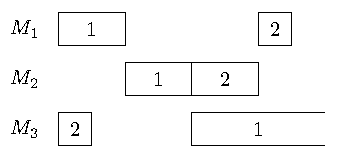
\includegraphics[scale=1]{figures/job-shop-delay.pdf}
  \caption{Example of an optimal schedule for Example~\ref{eg:job-shop}, shown
    as a Gantt chart. Each row $M_{i}$ corresponds to machine $i$ and each block
    numbered $j$ on this row represents the operation $(i,j)$. The dashed lines
    indicate unit time steps. Note that machine 2 is kept idle, while operation
    $(2,2)$ could have already been scheduled at time 1. Furthermore, for this
    particular instance, it can be checked that this is the unique optimal
    schedule.}
  \label{fig:job-shop-delay}
\end{figure}

\paragraph{Disjunctive graph.}

A commonly used representation of job shop problems is through their disjunctive
graph, which is a directed graph with vertices $\mathcal{N}$ corresponding to the
operations and two types of arcs.
%
The conjunctive arcs $\mathcal{C}$ are used to encode the predetermined machine
sequence of each job. Each such arc $(i, j) \rightarrow (k, j)$ encodes that job
$j$ should first be processed on machine $i$ before it is processed on machine
$k$.
%
When two distinct jobs $j_{1}$ and $j_{2}$ both require processing on the same
machine $i$, we say that they are conflicting.
%
The disjunctive arcs $\mathcal{D}$ are used to encode the possible choices of
resolving such conflicts, by deciding which of $j_{1}$ or $j_{2}$ visits $i$
first.
%
More specifically, let $j_{1}$ and $j_{2}$ be conflicting on some machine $i$,
then the nodes $(i,j_{1})$ and $(i,j_{2})$ are connected by two arcs in opposite
directions.

The disjunctive graph can also be used to encode (partial) solutions as follows.
%
It can be shown that each feasible solution corresponds to a selection
$\mathcal{O}$ of exactly one disjunctive arc from each pair such that the
induced graph $(\mathcal{N}, \mathcal{C} \cup \mathcal{O})$ is
acyclic~\cite{pinedoSchedulingTheoryAlgorithms2016}.
%
More precisely, consider two conflicting operations $(i,j_{1})$ and $(i,j_{2})$,
then $\mathcal{O}$ contains either $(i,j_{1}) \rightarrow (i,j_{2})$ or
$(i,j_{1}) \rightarrow (i,j_{2})$.
%
To illustrate this, the empty and complete disjunctive graphs for the instance
in Example~\ref{eg:job-shop} are shown in Figure~\ref{fig:disjunctive-graphs-job-shop}.

\begin{figure}
  \centering
  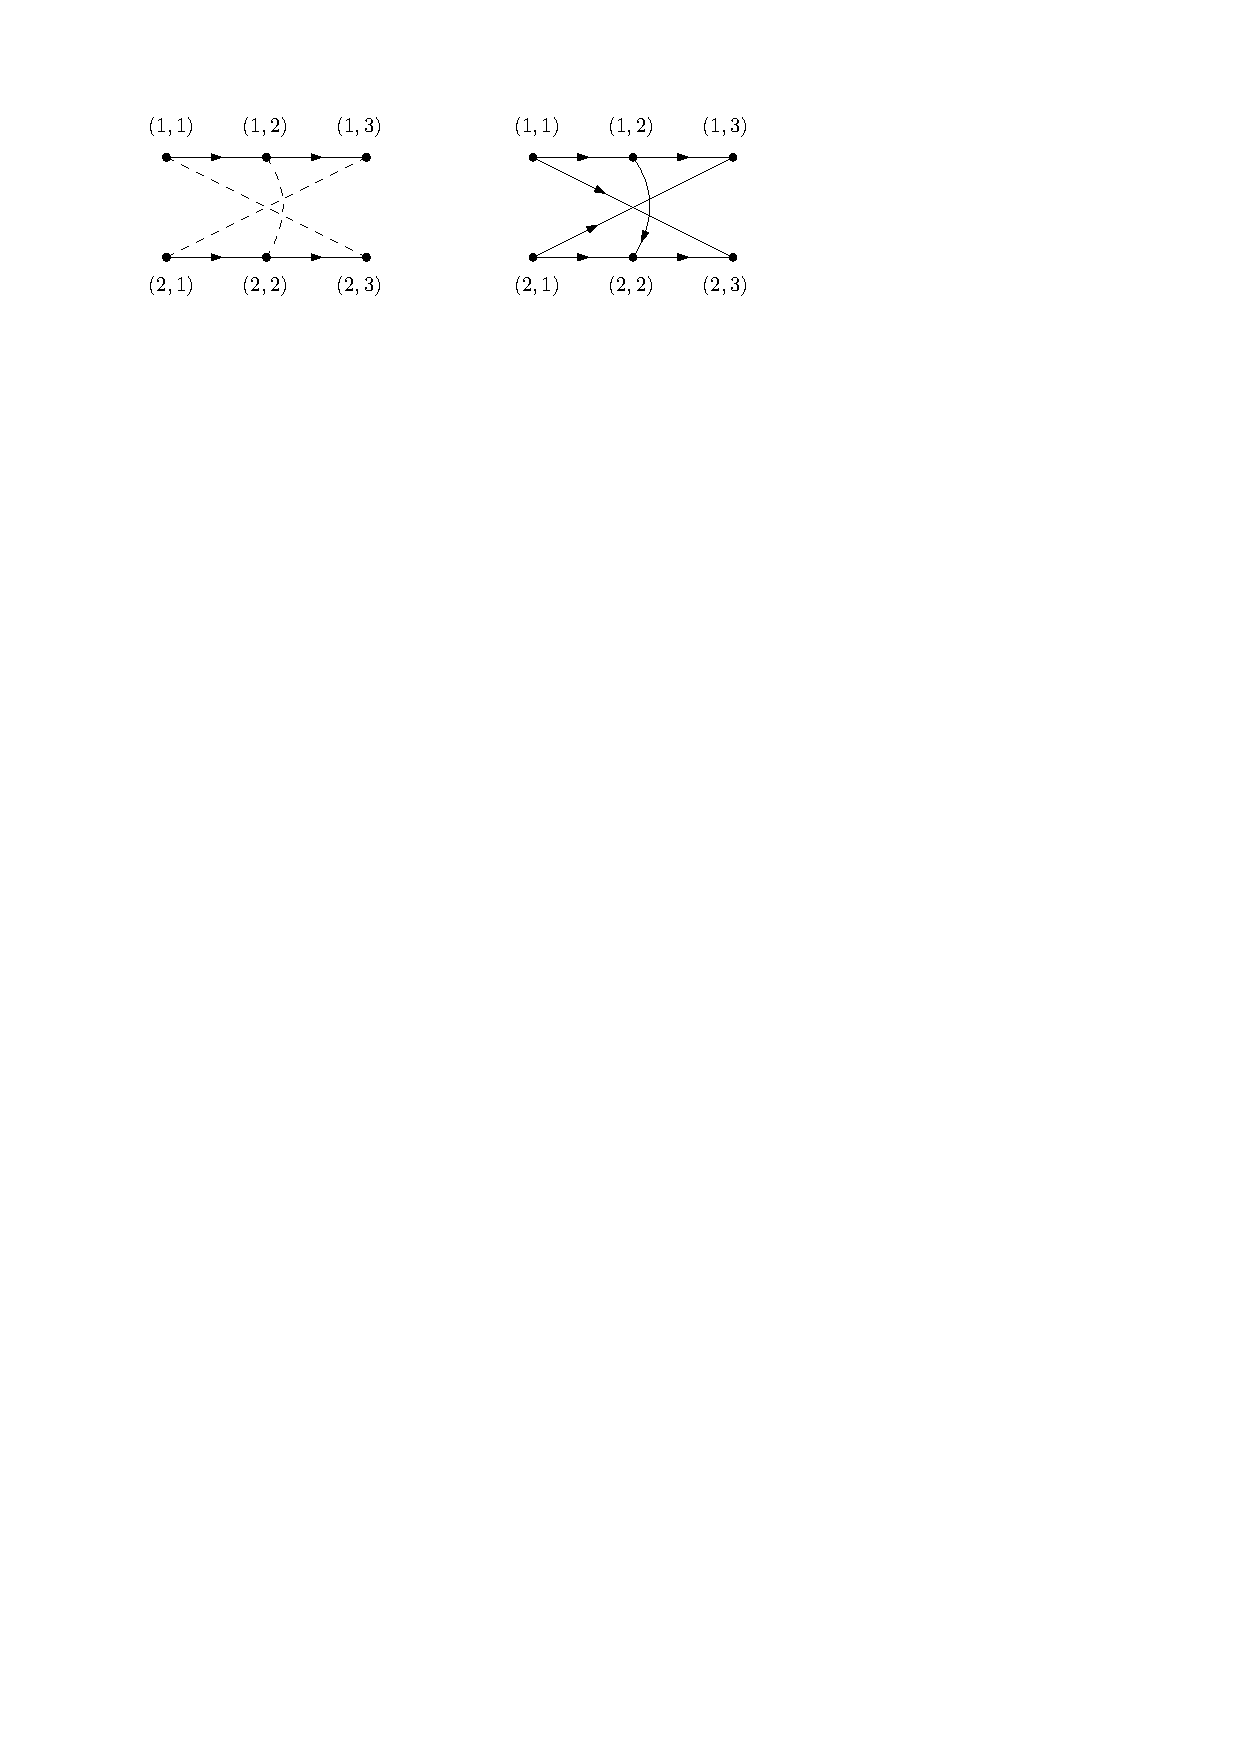
\includegraphics[scale=1]{figures/disjunctive_graph.pdf}
  \caption{Illustration of disjunctive graphs for Example~\ref{eg:job-shop}.
    Horizontal arrows represent conjunctive arcs. We used dashed lines to for
    the pairs of disjunctive arcs as dashed lines. The left graph corresponds to
    an empty selection $\mathcal{O} = \varnothing$ while the right graph shows
    the selection $\mathcal{O}$ that corresponds to the optimal schedule of
    Figure~\ref{fig:job-shop-delay}.}
  \label{fig:disjunctive-graphs-job-shop}
\end{figure}


\paragraph{Solution methods.}

Most job shop problems are very hard to solve. For example, the class of
problems $Jm|r_{j}|C_{\max}$ considered in Example~\ref{eg:job-shop} is known to
be NP-hard~\cite{grahamOptimizationApproximationDeterministic1979}, even without
release dates, which is denoted $Jm||C_{\max}$.
%
As a consequence, much effort has gone into developing good heurstics.
%
A type of heuristic that is often considered is to apply a so-called \emph{dispatching
rule} in order to build a schedule in a step-by-step fashion.
%
At each step, the rule chooses some job from all jobs with remaining unscheduled
operations and schedules this next operation at the earliest time possible,
given the current schedule.

A more principled way of solving job shop problems relies on the mathematical
programming framework.
%
We illustrate this for the problem $Jm|r_{j}|C_{\max}$ of
Example~\ref{eg:job-shop}. Using the notation of the disjunctive graph, the
problem can be concisely stated as
\[
\renewcommand{\arraystretch}{1.2}
\begin{NiceArray}{ r l @{} >{{}}c<{{}} @{} l @{} }
  \displaystyle \min_{y} & J(y) \\
  \text{such that } \; & y(s_{j},j) \leq r(j) && \quad \text{ for each job } j , \\
  &y(i, j) + p(i, j) \leq y(r, k) && \quad \text{ for each conjunction } (i,j) \rightarrow (r,k) \in \mathcal{C} , \\
  & y(i,j) + p(i,j) \leq y(i,k) & \\
  & \hspace{2em} \text{ or (not both) } && \quad \text{ for each disjunction } (i,j) \leftrightarrow (i,k) \in \mathcal{D} , \\
  & y(i,k) + p(i,k) \leq y(i,j) \\
  & y(i,j) \in \mathbb{R} && \quad \text{ for each operation } (i,j) \in \mathcal{N} .
\CodeAfter\SubMatrix.{4-1}{6-2}\}
\end{NiceArray}
\]
%
Note that this is almost an mixed-integer linear program (MILP).
%
Let $M > 0$ be some sufficiently large number and introduce a binary decision
variable $b_{(i,j)\leftrightarrow (i,k)} \in \{0,1\}$ for each pair of
disjunctive arcs, then the pair of disjunctive constraint can be rewritten to
\begin{align*}
  y(i,j) + p(i,j) &\leq y(i,k) + M b_{(i,j)\leftrightarrow (i,k)} , \\
  y(i,k) + p(i,k) &\leq y(i,j) + M (1 - b_{(i,j)\leftrightarrow (i,k)}) ,
\end{align*}
which is generally referred to as the \emph{big-M method}. The resulting MILP can
be solved by any off-the-shelf solver.

\chapter{Local search}\label{sec:local_search}

Without relying on systematic search methods like branch-and-bound, an often
employed method is to use some kind of local search heuristic.
%
The main idea is that the solution space can be organized based on some measure
of similarity. From the current solution, we only move to a neighboring solution
if it has a better objective value.
%
Next, give an example of such a neighborhood.

As seen in the previous sections, vehicles of the same route occur mostly in
platoons. For example, consider for example the route order
$\eta = (0, 1, 1, 0, 0, 1, 1, 1, 0, 0)$. This example has 5 platoons of
consecutive vehicles from the same route. The second platoon consists of two
vehicles from route 1.
%In general, let $P(\eta)$ denote the total number of platoons in $\eta$.
The basic idea is to make little changes in these platoons by moving vehicles at
the start and end of a platoon to the previous and next platoon of the same
route.
%
More precisely, we define the following two types of modifications to a route
order. A \textit{right-shift} modification of platoon $i$ moves the last vehicle of this
platoon to the next platoon of this route. Similarly, a \textit{left-shift} modification
of platoon $i$ moves the first vehicle of this platoon to the previous platoon
of this route.
%
We construct the neighborhood of a solution by performing every possible
right-shift and left-shift with respect to every platoon in the route order. For
illustration purposes, we have listed a full neighborhood for some example route
order in Table~\ref{tab:local_search}.

Now using this definition of a neighborhood, we must specify how the search
procedure visits these candidates.
In each of the following variants, the value of each neighbor is always computed.
%
The most straightforward way is to select the single best candidate in the
neighborhood and then continue with this as the current solution and compute its
neighborhood. This procedure can be repeated for some fixed number of times.
Alternatively, we can select the $k$ best neighboring candidates and then
compute the combined neighborhood for all of them. Then in the next step, we
again select the $k$ best candidates in this combined neighborhood and repeat.
The latter variant is generally known as \textit{beam search}.

\newcommand*{\one}{{\color{blue}1}}%
\newcommand*{\zero}{{\color{red}0}}%

\begin{table}
  \caption{Local search neighborhood of route order
    $\eta = (\zero, \one, \one, \zero, \zero, \one, \one, \one, \zero, \zero)$
    based on the left-shift and right-shift operations applied to every
    ``platoon'' in the current order.}
\label{tab:local_search}
\begin{center}
\begin{tabular}{c|c|c}
  platoon id  & left-shift & right-shift \\
  1 &  & (\one, \one, \zero, \zero, \zero, \one, \one, \one, \zero, \zero) \\
  2 & (\one, \zero, \one, \zero, \zero, \one, \one, \one, \zero, \zero) & (\zero, \one, \zero, \zero, \one, \one, \one, \one, \zero, \zero) \\
  3 & (\zero, \zero, \one, \one, \zero, \one, \one, \one, \zero, \zero) & (\zero, \one, \one, \zero, \one, \one, \one, \zero, \zero, \zero) \\
  4 & (\zero, \one, \one, \one, \zero, \zero, \one, \one, \zero, \zero) & (\zero, \one, \one, \zero, \zero, \one, \one, \zero, \zero, \one) \\
  5 & (\zero, \one, \one, \zero, \zero, \zero, \one, \one, \one, \zero) &
\end{tabular}
\end{center}
\end{table}



\chapter{Neural combinatorial optimization}\label{app:nco}

% maybe discuss traditional epsilon-approximation schemes?
% argue that it takes a lot of expert knowledge about the problem structure to design these

This section introduces the idea of applying a Machine Learning (ML) perspective
on Combinatorial Optimization (CO) problems, which has gained a lot of
attention\footnote{Pun not intended: a lot of recent works rely on neural attention architectures.} recently. One of the key ideas in this line of research is to treat problem
instances as data points and to use machine learning methods to approximately
map them to corresponding optimal solutions~\cite{bengioMachineLearningCombinatorial2020}.

% learning assumptions:
% supervised learning (expert labels) vs reinforcement learning (experience)
\paragraph{Algorithm execution as MDPs.}
It is very natural to see the sequential decision-making process of any
optimization algorithm in terms of the Markov Decision Process (MDP) framework,
where the environment corresponds to the internal state of the algorithm. From
this perspective, two main learning regimes can be distinguished.
% imitiation learning
Methods like those based on the branch-and-bound framework are
often computationally too expensive for practical purposes, so \textit{learning
  to imitate} the decisions taken in these exact algorithms might provide us
with fast approximations. In this approach, the ML model's performance is
measured in terms of how similar the produced decisions are to the
demonstrations provided by the expert.
% reinforcement learning
On the other hand, some problems do not even allow efficient exact methods, so it is
interesting to study solution methods that \textit{learn from experience}. An
interesting feature of this direction is that it enables the algorithm to implicitly
learn to exploit the hidden structure of the problems we want to solve.

% neural combinatorial optimization
Because neural networks are commonly used as encoder in these ML models for CO,
we will refer to this new field as \textit{Neural Combinatorial Optimization} (NCO).
%
A wide range of classical combinatorial optimization problems has already been
considered in this framework, so we briefly discuss the taxonomy used in the
survey~\cite{mazyavkinaReinforcementLearningCombinatorial2020}.
% principal vs. joint approach
One distinguishing feature is whether existing off-the-shelf solvers are used or
not. On the one hand, \textit{principal} methods are based on a parameterized algorithm
that is tuned to directly map instances to solutions, while \textit{joint} methods
integrate with existing off-the-shelf solvers in some way (see the
survey~\cite{lodiLearningBranchingSurvey2017} on integration with the
branch-and-bound framework). An illustrative example of the latter category are
the use of ML models for the branching heuristic or the selection of cutting
planes in branch-and-cut algorithms~\cite{tangReinforcementLearningInteger2020}.
% principal - construction vs. improvement (guided search)
The class of principal methods can be further divided into \textit{construction}
heuristics, which produce complete solutions by repeatedly extending partial
solutions, and \textit{improvement} heuristics, which aim at iteratively improving the
current solution with some tunable search procedure.


% learning algorithms:
% REINFOCE with baseline
% Fitting the neural mapping is often done using policy gradient methods (with
% baseline), e.g., with the classical REINFORCE algorithm.

% constraints in differentiable models

\paragraph{Constraint satisfaction.}
A major challenge in NCO is constraint satisfaction. For example, solutions
produced by neural construction policies need to satisfy the constraints of the
original combinatorial problem. To this end, neural network components have been
designed whose outputs satisfy some specific type of constraint, for example
being a permutation of the input~\cite{vinyalsPointerNetworks2017a}. Constraints can also be enforced by
the factorization of the mapping into repeated application of some policy. For
example, in methods for the classical traveling salesman problem, a policy is
defined that repeatedly selects the next node to visit. The constraint that
nodes may only be visited once can be easily enforced by ignoring the visited
nodes and taking the argmax among the model's probabilities for unvisited nodes.

% encoders:
% standard multilayer perceptron networks are not suited to encode order
% pointer networks
% graph neural networks

% backpropagation through solution
Instead of enforcing constraints by developing some tailored model architecture,
like construction and improvement heuristics, general methodologies have
recently been explored for the problem of constraint satisfaction in neural
networks. For example, the DC3 framework~\cite{dontiDC3LearningMethod2021}
employs two differentiable processes, completion and correction, to solve any
violations of equality or inequality constraints, respectively. The more recent
HardNet framework~\cite{minHardConstrainedNeuralNetworks2024} uses a closed-form
projection to map to feasible solutions under affine constraints and relies on a
differentiable convex optimization solver (e.g.,
OptNet~\cite{amosOptNetDifferentiableOptimization2021a}) when general convex
constraints are considered.

\paragraph{Neural job shop scheduling}
% examples for job-shop scheduling
Various NCO methods have already been studied for the Job Shop Scheduling Problem
(JSSP) with makespan objective, for which we now highlight some works that
illustrate some of the above classes of methods. A lot of the policies used in
these works rely on some graph neural network architecture, which is why the
survey~\cite{smitGraphNeuralNetworks2024} provides an overview based on this distinguishing feature.

% Tassel (principal construction, naive environment)
\paragraph{Dispatching rules.}
A very natural approach to model JSSP in terms of an MDP is taken
in~\cite{tasselReinforcementLearningEnvironment2021}, where a dispatching
heuristic is defined in an environment based on discrete scheduling time steps.
%
Every available job corresponds to a valid action and there is a so-called No-Op
action to skip to the next time step. States are encoded by some manually
designed features. They consider the makespan objective by proposing a dense
reward based on how much idle time is introduced compared to the processing time
of the job that is dispatched.
%
In some situation, some action can be proved to be always optimal (``non-final
prioritization''), in which case the policy is forced to take this action.
Additionally, the authors design some rules for when the No-Op action is not
allowed in order to prevent unnecessary idling of machines.
%
The proposed method is evaluated on the widely used
Taillard~\cite{taillardBenchmarksBasicScheduling1993} and
Demirkol~\cite{DEMIRKOL1998137} benchmarks, for which performance is compared to
static dispatching rules and a constraint programming (CP) solver, which is
considered cutting-edge.

% exact start times follow from order
From a scheduling theory
perspective~\cite{pinedoSchedulingTheoryAlgorithms2016}, it can be shown that
optimal schedules are completely characterized by the order of operations for
regular objectives (non-decreasing functions of the completion times). The start
times are computed from this order by a so-called \textit{placement rule}, so
considering discrete time steps introduces unnecessary model redundancy.

% Zhang construction heuristic (principal construction, based on order)

The seminal ``Learning to Dispatch'' (L2D)
paper~\cite{zhangLearningDispatchJob2020} proposes a construction heuristic for
JSSP with makespan objective. Their method is based on a dispatching policy that
is parameterized in terms of a graph neural network encoding of the disjunctive
graph belonging to a partial solution. Again, each action corresponds to
choosing for which job the next operation is dispatched. The rewards are based
on how much the lower bound on the makespan changes between successive states.
They use a Graph Isomorphism Network (GIN) architecture to parameterize both an
actor and critic, which are trained using the Proximal Policy Optimization (PPO)
algorithm. Using the Taillard and Demirkol benchmarks, they show that their
model is able to generalize well to larger instances.
% problem with dispatching mechanism
As we already alluded to above, this way of modeling the environment is better
suited to JSSP with regular objectives, because it does not explicitly determine
starting times.
%
They use a dispatching mechanism based on finding the earliest starting time of
a job, even before already scheduled jobs, see their Figure 2. By doing this,
they introduce symmetry in the environment: after operations
$O_{11}, O_{21}, O_{31}$ have been scheduled, both action sequences
$O_{22}, O_{32}$ and $O_{32}, O_{22}$ lead to exactly the same state $S_5$ shown
in their Figure 2. In this particular example, this means that it is impossible
to have $O_{11} \rightarrow O_{22} \rightarrow O_{32}$. In general, it is not
clear whether the resulting restricted policy is still sufficiently powerful, in
the sense that an optimal operation order can always be constructed.

% Zhang improvement heuristic (principal improvement)

\paragraph{Guided local search.}
Recently, the authors of L2D investigated an improvement heuristic for
JSSP~\cite{zhangDeepReinforcementLearning2024} with makespan objective.
%
This method is based on selecting a solution within the well-known $N_5$
neighborhood, which has been used in previous local search heuristics.
%
It is still not clear whether their resulting policy is complete, in the sense
that any operation order can be achieved by a sequence of neighborhood moves.
%
The reward is defined in terms of how much the solution improves relative to the
best solution seen so far (the ``incumbent'' solution). The policy is
parameterized using a GIN architecture designed to capture the topological
ordering of operations encoded in the disjunctive graph of solutions. They
propose a custom $n$-step variant of the REINFORCE algorithm in order to deal
with the sparse reward signal and long trajectories.
%
To compute the starting times based on the operation order, they propose a
dynamic programming algorithm, in terms of a message-passing scheme, as a more
efficient alternative to the classical recursive critical path method.
%
Our proposal for efficiently updating the current starting time lower bounds in
partial solutions can also be understood as a similar message-passing scheme,
but where only some messages are necessary.

\paragraph{Joint method.}
% Tassel (joint with CP solver)
An example of a joint method is given
in~\cite{tasselEndEndReinforcementLearning2023}, where the environment is stated
in terms of a Constraint Programming (CP) formulation. This allows the method to
be trained using demonstration from an off-the-shelf CP solver.


\chapter{Reinforcement learning}

For machine learning problems where data-collection is restricted in some way,
the supervised learning paradigm, i.e., learning from labeled examples, is
sometimes no longer appropriate or feasible.
%
Very generally, the reinforcement learning paradigm can viewed as a
generalization of supervised learning in which the data collection and selection
process is not fixed anymore.
%
The classical perspective is that of an \emph{agent} that tries to maximize some
cumulative \emph{rewward} signal when interacting in some \emph{environment},
which is formalized by the Markov Decision Process (MDP) model.
%
We refer the reader to~\cite{suttonReinforcementLearningIntroduction2018} for the commonly cited textbook introduction to RL
from this perspective.

\paragraph{Problem definition.}
Consider finite sets of states $\mathcal{S}$ and actions $\mathcal{A}$.
%
Given some current state $s$, the agent sends some action $a$ to the
environment, upon which it responds by providing some scalar reward signal $r$
and transitions to state $s'$, which happens with probablity $p(s', r | s, a)$.
%
By fixing a policy $\pi$, which is a function $\pi(a|s)$ that gives the
probablity of the agent choosing action $a$ in state $s$, we obtain the induced
\emph{state Markov chain} with transition probabilities
%
\begin{align*}
  \mathrm{Pr}(s \rightarrow s') = \sum_{a} \sum_{r} \pi(a|s) p(s', r | s, a) .
\end{align*}
Given some initial state distribution $h(s)$, we sample $S_{0} \sim h(s)$ and
use $S_{0}, S_{1}, S_{2}, \dots$ to denote some sample trajectory.
%
Moreover, we can also consider a more fine-grained Markov chain by considering
the sequence of states, actions and rewards
\begin{align*}
  S_{0}, A_{1}, R_{1}, S_{1}, A_{2}, R_{2}, S_{2}, \dots ,
\end{align*}
in which which the state Markov chain is naturally embedded. Such a sample
trajectory is also referred to as an \emph{episode}.
%
Let the corresponding \emph{return} at step $t$ be
defined as
\begin{align*}
  G_{t} = \sum_{k=t+1}^{\infty} R_{k} .
\end{align*}
By marking a subset of states as being \emph{final states}, we can consider finite episodes
\begin{align*}
  S_{0}, A_{1}, R_{1}, S_{1}, A_{2}, R_{2}, S_{2}, \dots S_{N},
\end{align*}
by using the convention that final states return zero reward and transition to
themselves almost surely.
%
For finite episodes, the goal is to find a policy $\pi$ that maximizes the
expected return $\mathbb{E}[G_{0}]$.

\paragraph{Solution methods.}
Most classical methods to find such an optimal policy $\pi$ can be categorized
as either being value-based or policy-based.
%
Value-based can be generally understood as producing some estimate $v(s)$ for
the expected return $\mathbb{E}[G_{0} | S_{0} = s]$. The optimal policy is then
parameterized in terms of these estimates $v(s)$.
%
In contrast, policy-based methods use a more direct parameterization of the
policy space and often rely on some kind of gradient-based optimization.
Specifically, let $\pi_{\theta}$ be some policy with parameters $\theta$, then we aim to
apply the gradient descent updating
\begin{align*}
  \theta \leftarrow \theta - \alpha \nabla \mathbb{E} [ G_{0} ]
\end{align*}
where $\alpha$ is referred to as the learning rate.
%
However, in almost all interesting situations, it is infeasible to compute the
gradient directly.

\paragraph{Induced Markov chain.}
For some fixed policy $\pi$ and initial state distribution $h$, we consider the
underlying \textit{induced Markov chain} over states. Because we are working with finite
episodes, the induced state process is a Markov chain with absorbing states.
%
We want to analyze how often states are visited on average, over multiple episodes.
%
To better understand what \textit{on average} means here, imagine that we link
together separate episodes to create a regular Markov chain without absorbing
states, in the following way: from each final state, we introduce state
transitions to the initial states according to distribution $h$, see also
Figure~\ref{fig:episodic_MC}. Furthermore, we will write $S_{t}^{(i)}$ to denote
the state at step $t$ of episode $i$.

\begin{figure}[h]
  \centering
  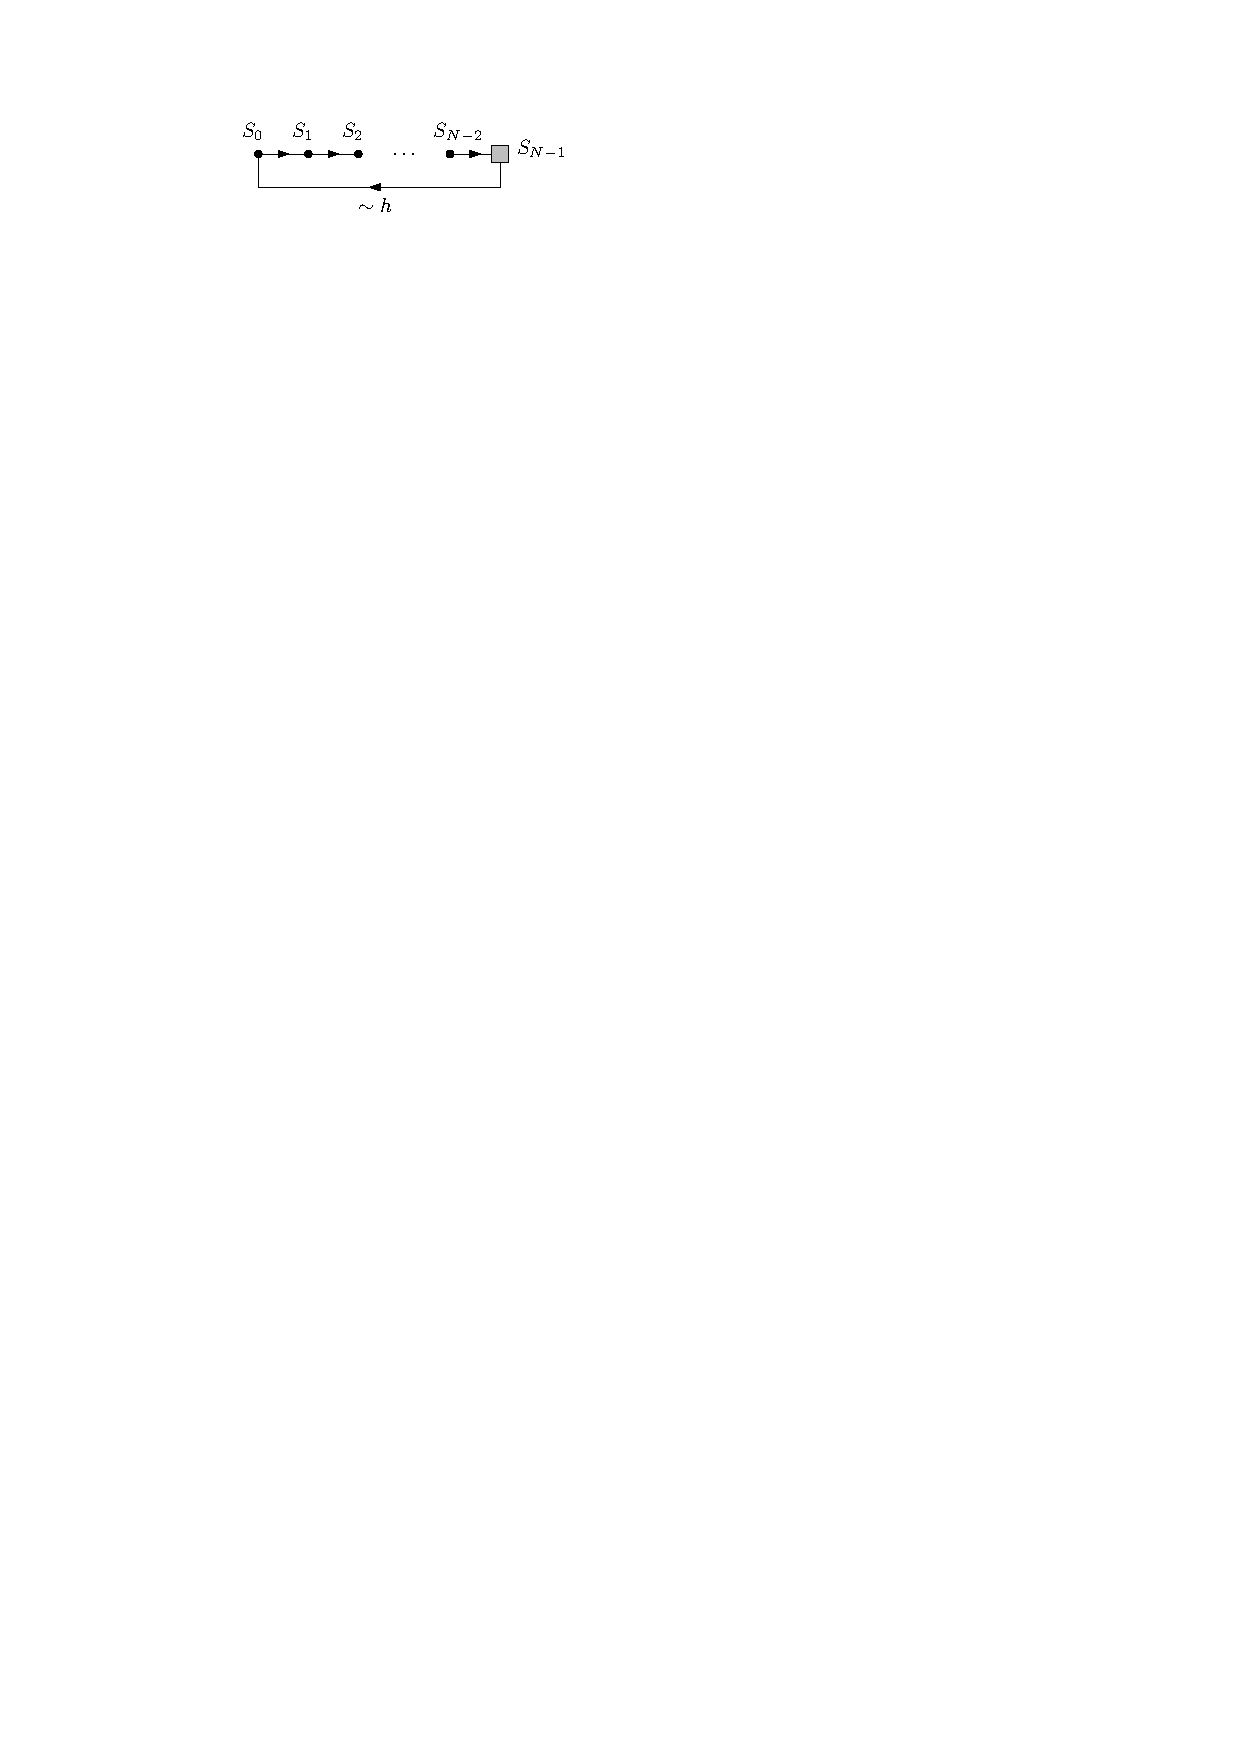
\includegraphics[width=0.4\textwidth]{figures/episodic_markov_chain.pdf}
  \caption{Illustration of the induced Markov chain when dealing with finite
    episodes. The next state after the final state, indicated as the grey
    rectangle, is sampled according to initial state distribution $h$.}
  \label{fig:episodic_MC}
\end{figure}


\section{Stationary distribution for finite episodes.}
Consider an absorbing Markov chain with transition matrix
\begin{align*}
  P_{xy} = \sum_{a} \pi(a | x) p(y | x, a) .
\end{align*}
There are $t$ transient states and $r$ absorbing states, so $P$ can be written
as
\begin{align*}
  P = \begin{pmatrix}
        Q & R \\
        \mathbf{0} & I_{r}
      \end{pmatrix} ,
\end{align*}
where $Q$ is a $t$-by-$t$ matrix, $R$ is a nonzero $t$-by-$r$ matrix, $I_{r}$ is
the $r$-by-$r$ identify matrix and $\mathbf{0}$ is the zero matrix.
%
Observe that $(Q^{k})_{xs}$ is the probability of reaching state $s$ in $k$
steps without being absorbed, starting from state $x$. Hence, the expected
number of visits to state $s$ without being absorbed, starting from state $x$,
is given by
\begin{align*}
  \eta(s | x) := \sum_{k=0}^{\infty} (Q^{k})_{xs} .
\end{align*}
%
Writing this in matrix form $N_{xs} = \eta(s | x)$, we can use the following
property of this so-called Neumann series, to obtain
\begin{align*}
  N = \sum_{k=0}^{\infty} Q^{k} = {(I_{t} - Q)}^{-1} .
\end{align*}
Now we can derive two equivalent equations
\begin{align*}
  N = (I_{t} - Q)^{-1} \iff
  \begin{cases}
    N (I_{t} - Q) = I_{t} \iff N = I_{t} + NQ ,
    \quad  \text{ or }  \\
    (I_{t} - Q) N = I_{t} \iff N = I_{t} + QN . \\
  \end{cases}
\end{align*}
%
Expanding the first equation in terms of matrix entries $N_{xs} = \eta(s | x)$
gives
\begin{align*}
  \eta(s | x) &= \mathds{1}\{ x = s \} + \sum_{y}  \eta(y | x) Q_{ys} \\
  &= \mathds{1}\{ x = s \} +  \sum_{y}\eta(y | x) \sum_{a} \pi(a | y) p(y | x, a)
\end{align*}
and similarly, the second equation gives
\begin{align*}
  \eta(s | x) &= \mathds{1}\{ x = s \} + \sum_{y} Q_{xy} \eta(s | y) \\
  &= \mathds{1}\{ x = s \} +  \sum_{a} \pi(a | x) \sum_{y} p(y | x, a) \eta(s | y)
\end{align*}
%
Now since the initial state is chosen according to distribution $h$, the
expected number of visits $\eta(s)$ to state $s$ in some episode is given by
\begin{align*}
  \eta(s) = \sum_{x} h(x) \eta(s | x) ,
\end{align*}
or written in matrix form $\eta = hN$, where $\eta$ and $h$ are row vectors.
%
Therefore, we can also work with the equations
\begin{align*}
  \begin{cases}
  hN = h + hNQ , \quad \text{ or } \\
  hN = h + hQN ,
  \end{cases}
\end{align*}
which are generally called \textit{balance equations}.
% or written in terms of matrix entries, respectively,
% \begin{align*}
%   \begin{cases}
%   \eta(s) = h(s) + \sum_{x} h(x) \sum_{y} \eta(y|x) \sum_{a} \pi(a|y)p(s|y, a) , \text{ or } \\
%   \eta(s) = h(s) + \sum_{x} h(x) \sum_{a} \pi(a | x) \sum_{y} p(y | x, a) \eta(s | y) .
%   \end{cases}
% \end{align*}
By writing the first variant as $\eta = h + \eta Q$ and expanding the matrix
multiplication, we obtain
\begin{align*}
  \eta(s) = h(s) + \sum_{y} \eta(y) \sum_{a} \pi(a|y)p(s|y,a) .
\end{align*}
%
Through appropriate normalization of the expected number of visits, we obtain
the average fraction of time spent in state $s$, given by
\begin{align*}
  \mu(s) = \frac{\eta(s)}{\sum_{s'} \eta(s')} .
\end{align*}

\paragraph{Sampling.}

Suppose we have some function $f : \mathcal{S} \rightarrow \mathbb{R}$ over
states and we are interested in estimating $\mathbb{E}_{S_{t}^{(i)} \sim \mu}[f(S_{t}^{(i)})]$.
%
We can just take random samples of $S_{t}^{(i)}$, by sampling initial state
$S_{0}^{(i)} \sim h$ and then \textit{rolling out} $\pi$ to obtain
\begin{align*}
\tau^{(i)} = (S_{0}^{(i)},A_{0}^{(i)},R_{1}^{(i)},S_{1}^{(i)},A_{1}^{(i)},R_{2}^{(i)},S_{2}^{(i)}, \dots, S_{N^{(i)}-1}^{(i)}) \sim \pi(\tau^{(i)} | S_{0}^{(i)}),
\end{align*}
where $N^{(i)}$ denotes the total number of states visited in this episode.
%
Given $M$ such episode samples, we compute the estimate as
\begin{align*}
  \mathbb{E}_{S_{t}^{(i)} \sim \mu} [ f(S_{t}^{(i)}) ] \approx \left( \sum_{i=1}^{M} \sum_{t=0}^{N^{(i)} - 1} f(S_{t}^{(i)}) \right) / \left( \sum_{i=1}^{M} N^{(i)} \right) .
\end{align*}

Observe that the analysis of the induced Markov chain can be extended to
explicitly include actions and rewards as part of the state and derive the
stationary distribution of the resulting Markov chain. However, we do not need
this distribution explicitly in practice, because we can again use episode
samples $\tau^{(i)}$. To keep notation concise, we will from now on denote this
type of expectation as $\mathbb{E}_{\tau \sim h,\pi}[f(\tau)]$ and omit episode
superscripts.
%
Using this new notation, note that the average episode length is given by
\begin{align*}
  \mathbb{E}_{h, \pi} [ N ]= \sum_{s'} \eta(s') .
\end{align*}

\section{Policy gradient estimation}

Let $v_{\pi_{\theta}} = \mathbb{E}_{h,\pi_{\theta}}[G_{0}]$ denote the expected
episodic reward under policy $\pi$, where $G_{t}$ is called the reward-to-go at
step $t$, which is defined as
\begin{align*}
  G_{t} := \sum_{k=t+1}^{\infty} R_{k} .
\end{align*}
The main idea of policy gradient methods is to update the policy parameters
$\theta$ in the direction that increases the expected episodic reward the most. This
means that the policy parameters are updated as
\begin{align*}
  \theta_{k+1} = \theta_{k} + \alpha \nabla v_{\pi_{\theta}} ,
\end{align*}
where $\alpha$ is the learning rate and the gradient is with respect to
$\theta$. Instead of trying to derive or compute the gradient exactly, we often
use some statistical estimate based on sampled episode. The basic policy
gradient algorithm is to repeat the three steps

\vspace{1em}
\noindent
\hspace*{1em} \texttt{1. sample $M$ episodes $\tau^{(1)}, \dots, \tau^{(M)}$ following $\pi_{\theta}$,}\\
\hspace*{1em} \texttt{2. compute gradient estimate $\widehat{\nabla v_{\pi_{\theta}}}(\tau^{(1)}, \dots, \tau^{(M)})$,} \\
\hspace*{1em} \texttt{3. update $\theta \leftarrow \theta + \alpha \widehat{\nabla v_{\pi_{\theta}}}$.}

\paragraph{REINFORCE estimator.}

We will now present the fundamental policy gradient theorem, which essentially
provides a function $f$ such that
\begin{align*}
  \nabla v_{\pi_{\theta}} = \mathbb{E}_{\tau \sim h,\pi_{\theta}}[f(\tau)] ,
\end{align*}
which allows us to estimate the policy gradient using episode samples.
%
To align with the notation
of~\cite{suttonReinforcementLearningIntroduction2018}, we write
$\mathrm{Pr}(x \rightarrow s, k, \pi) := (Q^{k})_{xs}$, for the probability of
reaching state $s$ in $k$ steps under policy $\pi$, starting from state some
$x$, so that the expected number of visits can also be written as
\begin{align*}
  \eta(s) = \sum_{x} h(x) \sum_{k=0}^{\infty} \mathrm{Pr}(x \rightarrow s, k, \pi)
\end{align*}
%
As proven in the chapter on policy gradient methods
in~\cite{suttonReinforcementLearningIntroduction2018}, the gradient of the value
function for a fixed initial state $s_0$ with respect to the parameters is given
by
\begin{align}
  \nabla v_{\pi}(s_{0}) = \sum_{s} \sum_{k=0}^{\infty} \mathrm{Pr}(s_{0} \rightarrow s, k, \pi) \sum_{a} q_{\pi}(s,a) \nabla \pi(a|s) .
\end{align}
When choosing the initial state $s_{0}$ according to some distribution
$h(s_{0})$, we verify that the final result is still the same as in
\cite{suttonReinforcementLearningIntroduction2018}:
\begin{subequations}
\begin{align}
  \nabla v_{\pi} :=& \nabla \mathbb{E}_{s_{0} \sim h}[v_{\pi}(s_{0})] \\
  =& \sum_{s_{0}} h(s_{0}) \sum_{s} \sum_{k=0}^{\infty} \mathrm{Pr}(s_{0} \rightarrow s, k, \pi) \sum_{a} q_{\pi}(s,a) \nabla \pi(a|s) \\
  =& \sum_{s} \eta(s) \sum_{a} q_{\pi}(s,a) \nabla \pi(a|s) \\
  =& \sum_{s'} \eta(s') \sum_{s} \mu(s) \sum_{a} q_{\pi}(s,a) \nabla \pi(a|s) \\
  \propto& \sum_{s} \mu(s) \sum_{a} q_{\pi}(s,a) \nabla \pi(a|s) ,
\end{align}
\end{subequations}
where the constant of proportionality is just the average episode length.
%
Because we do not know $\mu$ or $q_{\pi}$ explicitly, we would like to estimate
$\nabla v_{\pi}$ based on samples. If we sample episodes according to $h$ and
$\pi$ as explained above, we encounter states according to $\mu$, so we have
\begin{subequations}
\begin{align}
  \nabla v_{\pi} &\propto \mathbb{E}_{h, \pi} \left[ \sum_{a} q_{\pi}(S_{t}, a) \nabla\pi(a | S_{t}) \right] \\
  &= \mathbb{E}_{h, \pi} \left[ \sum_{a} \pi(a | S_{t}) q_{\pi}(S_{t}, a) \frac{\nabla \pi(a | S_{t})}{\pi(a | S_{t})} \right] \\
  &= \mathbb{E}_{h, \pi} \left[ q_{\pi}(S_{t}, A_{t}) \frac{\nabla \pi(A_{t} | S_{t})}{\pi(A_{t}| S_{t})} \right] \\
  &= \mathbb{E}_{h, \pi} \left[ G_{t} \nabla \log \pi(A_{t} | S_{t}) \right] .
  \label{eq:estimator1}
\end{align}
\end{subequations}

\paragraph{Baseline.}
Let $b(s)$ be some function of the state $s$ only, then we have for any $s \in \mathcal{S}$
\begin{align}
  \sum_{a} b(s) \nabla \pi(a | s) = b(s) \nabla \sum_{a} \pi(a | s) = b(s) \nabla 1 = 0 .
\end{align}
This yields the so-called REINFORCE estimate with \textit{baseline}
\begin{subequations}
\begin{align}
  \nabla v_{\pi} &\propto \sum_{s} \mu(s) \sum_{a} (q_{\pi}(s, a) + b(s)) \nabla \pi(a | s) \\
          &= \mathbb{E}_{h, \pi} \left[ \bigl(q_{\pi}(S_{t}, A_{t}) + b(S_{t}) \bigr) \nabla \log \pi(A_{t} | S_{t}) \right] \\
  &= \mathbb{E}_{h, \pi} \left[ \bigl(G_{t} + b(S_{t}) \bigr) \nabla \log \pi(A_{t} | S_{t}) \right] .
  \label{eq:estimator2}
          %&= \mathbb{E}_{h, \pi} \left[ \bigl(G_{t} + b(S_{t}) \bigr) \nabla \log \pi(A_{t} | S_{t}) \right]
\end{align}
\end{subequations}
%
Although estimates~\eqref{eq:estimator1} and~\eqref{eq:estimator2} are both equivalent in terms of their expected
value, they may differ in higher moments, which is why an appropriate choice of
$b$ can make a lot of difference in how well the policy gradient algorithm
converges to an optimal policy.
%
As a specific baseline, consider the expected cumulative sum of rewards up to
step the current step $t$, defined as
\begin{align}
  b(s) = \mathbb{E}_{h,\pi} \left[ \sum_{k=1}^{t} R_{k} \Big| S_{t} = s \right],
\end{align}
then observe that
\begin{subequations}
\begin{align}
  q_{\pi}(s, a) + b(s) &= \mathbb{E}_{h,\pi}\left[ \sum_{k=t+1}^{\infty} R_{k} \Big| S_{t} = s , A_{t} = a \right] + \mathbb{E}_{h,\pi}\left[ \sum_{k=1}^{t} R_{k} \Big| S_{t} = s \right] \\
                     &= \mathbb{E}_{h,\pi}\left[ \sum_{k=1}^{\infty}  R_{k} \Big| S_{t} = s, A_{t} = a \right] \\
                     &= \mathbb{E}_{h,\pi} [ G_{0} | S_{t} = s, A_{t} = a ] ,
\end{align}
\end{subequations}
which is just the expected total episodic reward.
%
Now define function $f$ to be
\begin{subequations}
\begin{align}
  f(s, a) := (q_{\pi}(s, a) + b(s))\nabla \log \pi(a | s) &= \mathbb{E}_{h,\pi} \left[ G_{0} | S_{t} = s, A_{t} = a \right] \nabla \log \pi(a | s) \\
  &= \mathbb{E}_{h,\pi} \left[ G_{0} \nabla \log \pi(a | s) | S_{t} = s, A_{t} = a \right] ,
\end{align}
\end{subequations}
then applying the law of total expectation yields
\begin{align}
  \nabla v_{\pi} \propto \mathbb{E}_{h,\pi}[f(S_{t}, A_{t})] =  \mathbb{E}_{h, \pi} \left[ G_{0} \nabla \log \pi(A_{t} | S_{t}) \right] .
\end{align}



\chapter{Miscellaneous}\label{app:misc}

\minimalnode*
\begin{proof}
  For sake of contradiction, suppose there is no such minimal node, so every
  $v \in V$ has an incoming arc. Pick some arbitrary $v_0 \in V$, then there
  must exist $v_1 \in V$ such that $v_1 \rightarrow v_0$. Again, $v_1$ must have
  an incoming, so we can pick $v_2 \in V$ such that $v_2 \rightarrow v_1$. We
  can continue picking such predecessor as long as we want, obtaining a sequence
  $v_0, v_1, \dots, v_n$. Since there are only finitely many nodes, if we take
  the length $n$ of this sequence large enough, we must eventually pick a node
  twice, say $v_k = v_m$ for some $m < k \leq n$, but then we have
  $v_k \rightarrow v_{k-1} \rightarrow \cdots \rightarrow v_m = v_k$, which
  shows $\mathcal{G}$ has a cycle.

  To show that $\mathcal{G}$ has a topological order, consider the following
  procedure. Starting with $\mathcal{G}_0 := \mathcal{G}$ we select some minimal
  node $v_1$. We remove $v_1$ and all its outgoing edges from the graph to
  obtain a new graph $\mathcal{G}_1$, which is still a DAG, so there must be
  some minimal node $v_2$. We can repeat this procedure until
  $\mathcal{G}_{N}$ is an empty graph to obtain a sequence $v_1, \dots, v_N$.
  Suppose $v_i \rightarrow v_j$ in $\mathcal{G}$, then $v_i$ must appear earlier
  in the sequence than $v_j$, because otherwise $v_i$ was not a minimal element
  at the time it was picked.
\end{proof}

\lblemma*
\begin{proof}
  We prove that $y$ is a feasible solution to~\eqref{eq:active_schedule} by showing that it satisfies~\eqref{eq:feasible-schedule}.
  %
  First of all, since $\pi_1$ is a minimal node of $G(\mathcal{O})$, we have
  $\mathcal{N}^-(\pi_1) = \varnothing$, so feasibility
  condition~\eqref{eq:feasible-schedule} is trivially satisfied with equality by
  the definition $y_{\pi_1} = a_{\pi_1}$. We proceed inductively by showing
  that, for any further $i = \pi_t$ and $j = \pi_{t+1}$, we have
  \begin{align}
    \label{eq:max-arc}
    y_i + w(i,j) = \max_{v \in \mathcal{N}^-(j)} y_v + w(v,j)
  \end{align}
  so that the definition of $y_j$ through~\eqref{eq:lb-computation} also
  satisfies~\eqref{eq:feasible-schedule} with equality.
  %
  Hence, uniqueness of $y(\mathcal{O}) = y$ simply follows from the fact that
  $y_j$ satisfies~\eqref{eq:feasible-schedule} with equality for every
  $j \in \mathcal{N}$.

  For the inductive step, we show $y_{i} + w(i,j) \geq y_{v} + w(v,j)$ for any
  $v \in \mathcal{N}^{-}(j) \setminus \{i\}$ for the cases illustrated in
  Figure~\ref{fig:lb-computation}.
  %
  Suppose $i$ and $j$ are connected via a disjunctive arc $(i,j) \in \mathcal{C}$,
  then any other in-neighbor $v \in \mathcal{N}^-(j) \setminus \{ i \}$ must
  belong to a different route, so that $(v,j) \in \mathcal{O}$. Because $i$ and
  $j$ are on the same route and $i$ is the immediate predecessor of $j$ in the
  topological order, we must also have $(v,i) \in \mathcal{O}$. Therefore, we have
  \begin{align*}
    y_i + w(i,j) = y_i + \rho \geq y_v + \sigma + \rho > y_v + \sigma = y_v + w(v,j) .
  \end{align*}
  %
  Otherwise, $i$ and $j$ are connected by a disjunctive arc
  $(i,j) \in \mathcal{O}$. Let $v \in \mathcal{N}^-(j) \setminus \{i\}$, then if
  $v$ is on the same route as $j$, they are connected by a conjunctive arc
  $(v,j) \in \mathcal{C}$, so we must have $(v,i) \in \mathcal{O}$, again because
  $i$ is the immediate predecessor of $j$. Hence, we have
  \begin{align*}
    y_i + w(i,j) = y_i + \sigma \geq y_v + 2 \sigma > y_{v} + \rho = y_{v} + w(v,j) .
  \end{align*}
  %
  If $(v, j) \in \mathcal{O}$ with $r(v) \neq r(i)$, then it follows that
  $(v,i) \in \mathcal{O}$, so that
  \begin{align*}
    y_{i} + w(i,j) = y_i + \sigma \geq y_v + 2\sigma > y_v + \sigma = y_v + w(v,j) .
  \end{align*}
  If $(v, j) \in \mathcal{O}$ with $r(v) = r(i)$, then there is a path of
  conjunctive arcs between $v$ and $i$, from which it follows that
  $y_i \geq y_{v} + \rho$, so that
  \begin{align*}
    y_i + w(i,j) = y_i + \sigma \geq y_v + \sigma + \rho > y_v + w(v, j) . & \qedhere
  \end{align*}
\end{proof}

\begin{figure}
  \centering
  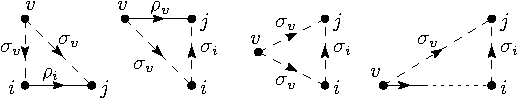
\includegraphics[width=0.8\textwidth]{figures/single/lower-bound-lemma.pdf}
  \caption{Sketch of the four cases distinguished in the proof of Lemma~\ref{lemma:lb-computation}. Arc
    weights are indicated by $\sigma$ and $\rho$. Conjunctive arcs $\mathcal{C}$
    are drawn with solid lines and disjunctive arcs $\mathcal{O}$ are drawn with
    dashed lines. The dotted line in the rightmost figure represent a chain of
    conjunctive arcs.}\label{fig:lb-computation}
\end{figure}

\begin{lemma}\label{lemma:inf-continuous}
  Let $f : X \times Y \rightarrow \mathbb{R}$ be some continuous function. If
  $Y$ is compact, then the function $g : X \rightarrow \mathbb{R}$, defined as
  $g(x) = \inf \{ f(x,y) : y\in Y\}$, is also continuous.
\end{lemma}

\begin{lemma}\label{lemma:levelset}
  Let $f :\mathbb{R}^{n} \rightarrow \mathbb{R}^{m}$ be continuous and
  $y \in \mathbb{R}^{m}$, then the level set $N := f^{-1}(\{ y \})$ is a closed
  subset of $\mathbb{R}^{n}$.
\end{lemma}
\begin{proof}
  For any $y' \neq y$, there exists an open neighborhood $M(y')$ such that
  $y \notin M(y')$. The preimage $f^{-1}(M(y'))$ is open by continuity.
  Therefore, the complement
  $N^{c} = \{ x : f(x) \neq y \} = \cup_{y' \neq y} f^{-1}(\{y'\}) = \cup_{y' \neq y} f^{-1}(M(y'))$
  is open.
\end{proof}


\note{The following definition might be helpful in deriving the buffer constraint.\dots}

\paragraph{Acceleration boundary.}
Before we present the decomposition, we first define an auxiliary upper
boundary.
%
Similar to how we generalized the entry boundary $\check{x}$ to the deceleration
boundary in Section~\ref{sec:deceleration-boundary}, we now generalize the exit
boundary $\hat{x}$ to obtain the \emph{acceleration boundary}.
%
Because the derivation is completely analogous, we will only present the
resulting expressions.
%
Let $x \in \mathcal{D}[a,b]$ be some smooth trajectory, then the acceleration
boundary $x^{+}[\xi]$ of $x$ at some $\xi \in [a,b]$ is defined as the
right-hand side of the inequality
\begin{align}
  x(t) \leq x(\xi) + \int_{\xi}^{t} \{\dot{x}(\xi) + \bar{\omega} (\tau - \xi) \}_{[0,1]} \diff \tau =: x^{+}[\xi](t) ,
\end{align}
which holds for every $t \in [a,b]$.
%
Observe that the exit boundary can now be written as the restricted acceleration
boundary $\hat{x} = (x^{+}[b])|_{[a,b]}$.
%
Similar to definition~\eqref{eq:def-x-}, we define
\begin{align}
  x^{+}[p,v,\xi](t) := p + \int_{\xi}^{t}\{ v + \bar{\omega}(\tau - \xi)\}_{[0,1]} \diff \tau ,
\end{align}
such that $x^{+}[\xi](t) = x^{+}[x(\xi),\dot{x}(\xi),\xi](t)$ and
%
similar to~\eqref{eq:x-}, we calculate
\begin{align}
  x^{+}[p,v,\xi](t) = p +
  \begin{cases}
    \dots &\text{ for } t \leq \bar{\delta}_{0} , \\
    \dots &\text{ for } t \in [\bar{\delta}_{0}, \bar{\delta}_{1} ] , \\
    \dots &\text{ for } t \geq \bar{\delta}_{1} ,
  \end{cases}
\end{align}
with $\bar{\delta}_{0} := $ and $\bar{\delta}_{1} := $.

\note{
Recall the definition of $\hat{x}$ in equation~\eqref{eq:hat-x}. By carefully
handling the $\max\{\cdot\}$, we can expand this expression as
\begin{align}
  \hat{x}(t) =
  \begin{cases}
    B - b + t + \bar{\omega} (b-t)^{2} / 2 &\text{ for } t \geq b - 1/\bar{\omega} , \\
    B - 1/(2\bar{\omega}) &\text{ for } t \leq b - 1/\bar{\omega} .
  \end{cases}
\end{align}
}

\end{document}

% add extra flag when compiling from emacs
% Local Variables:
% TeX-command-extra-options: "-shell-escape"
% End:
